\documentclass[12pt,PhD]{Thesis}



% ******** vmargin settings *********
\usepackage{vmargin} %This give you full control over the used page area, it maybe not the idea method in Latex to do so, but I wanted to reduce to amount of white space on the page
\setpapersize{A4}
%\setmargins{3.5cm}%			%linker Rand, left edge
%	  {1cm}%     %oberer Rand, top edge
%           {14.7cm}%		%Textbreite, text width
%           {23.42cm}%   %Texthoehe, text hight
%           {14pt}%			%Kopfzeilenhöhe, header hight
%t           {1cm}%   	  %Kopfzeilenabstand, header distance
%           {0pt}%				%Fußzeilenhoehe footer hight
%           {2cm}%    	  %Fusszeilenabstand, footer distance   


%Defining text font profile
\usepackage{t1enc} % as usual




\usepackage[utf8]{inputenc} % as usual
\usepackage{times}	
\usepackage{mathcomp, subfigure}
\usepackage{amssymb}
\usepackage{amsmath}
\usepackage[pdftex]{graphicx}
\usepackage{cleveref}
\usepackage{longtable}
\usepackage[refpage]{nomencl}
\renewcommand{\nomname}{List of Notations}
\renewcommand*{\pagedeclaration}[1]{\unskip\dotfill\hyperpage{#1}}
\makenomenclature
\usepackage{makeidx}
\nomenclature{$\mathcal{L}$}{Luminosity at a collision point}
\nomenclature{$\sigma_{p}$}{Production cross section for a particle reaction}
\nomenclature{$N_{b}$}{Bunch population. b replaced by 1 or 2 for the case of colliding beams}
\nomenclature{$f_{rev}$}{Revolution frequency of the accelerator}
\nomenclature{$n_{b}$}{The number of bunches in the accelerator. In the case of colliding beams it it the number of colliding bunches}
\nomenclature{$\sigma_{x,y}$}{Gaussian bunch sigma for the transverse cross-section in the horizontal and vertical planes}
\nomenclature{$\sigma_{x,y}$}{Gaussian bunch sigma for the transverse cross-section in the horizontal and vertical planes}
\nomenclature{$e$}{Charge of an electron}
\nomenclature{$I_{b}$}{DC beam current}
\nomenclature{$(\rho , \theta , z)$}{Coordinate system of an ideal on-momentum particle}
\nomenclature{$(x , y , z)$}{Coordinate system comoving with the on-momentum particle}
\nomenclature{$q$}{Charge of a particle}
\nomenclature{$\mathbf{E} = (E_{x}, E_{y}, E_{z})$}{The electric field components relative to the coordinate system following the on-momentum particle}
\nomenclature{$\mathbf{B} = (B_{x}, B_{y}, B_{z})$}{The magnetic induction (referred to as the magnetic field in the text due to convention) components relative to the coordinate system following the on momentum particle}
\nomenclature{$\mathbf{v}$}{Particle velocity}
\nomenclature{$m$}{Particle Mass}
\nomenclature{$\gamma$}{Relativistic factor}
\nomenclature{$\beta$}{Particle velocity normalised by the speed of light}
\nomenclature{$p$}{Particle momentum}
\nomenclature{$k_{f}$}{Focal strength of a quadrupole magnet}
\nomenclature{$c$}{Speed of light in vacuum($=$299792458 m/s)}
\nomenclature{$\omega$}{Angular velocity or angular frequency}
\nomenclature{$k$}{Wave number}
\nomenclature{$(x_{1}, y_{1},z_{1})$}{The coordinates of the source or inducing particle of a wakefield}
\nomenclature{$(x_{2}, y_{2}, z_{2})$}{The coordinates of the test or witness particle of a wakefield}
\nomenclature{$q_{1}$}{Charge of the source or inducing particle of a wakefield}
\nomenclature{$q_{1}$}{Charge of the test or witness particle of a wakefield}
\nomenclature{$E_{\parallel}$}{The longitudinal component of an electric field}
\nomenclature{$\mathbf{E}_{\perp}$}{The perpendicular components of an electric field}
\nomenclature{$B_{\parallel}$}{The longitudinal component of a magnetic field}
\nomenclature{$\mathbf{B}_{\perp}$}{The perpendicular components of a magnetic field}
\nomenclature{$F_{\parallel}$}{The longitudinal component of a force}
\nomenclature{$\mathbf{F}_{\perp}$}{The perpendicular components of a force}
\nomenclature{$\tau$}{The time between the source and witness particle in the comoving reference frame}
\nomenclature{$k_{loss}$}{The loss factor of a single particle wakefield}
\nomenclature{$w_{\parallel}$}{The longitudinal wake function}
\nomenclature{$W_{\parallel}$}{The longitudinal wake function of a bunch or wakepotential}
\nomenclature{$w_{\perp}$}{The transverse wake function}
\nomenclature{$W_{\perp}$}{The transverse wake function of a bunch or trasnverse wakepotential}
\nomenclature{$j$}{imaginary number $-\sqrt{-1}$}
\nomenclature{$Z_{\parallel}$}{The total longitudinal impedance}
\nomenclature{$Z_{\perp}$}{The total transverse impedance}
\nomenclature{$Z_{dip, x}$ or $Z_{dipolar, x}$}{The horizontal dipolar or driving impedance}
\nomenclature{$Z_{dip, y}$ or $Z_{dipolar, y}$}{The vertical dipolar or driving impedance}
\nomenclature{$Z_{quad, x}$ or $Z_{quadrupolar, x}$}{The horizontal quadrupolar or detuning impedance}
\nomenclature{$Z_{quad, y}$ or $Z_{quadrupolar, y}$}{The vertical quadrupolar or detuning impedance}
\nomenclature{$Z_{const, x}$ or $Z_{constant, x}$}{The horizontal constant impedance}
\nomenclature{$Z_{const, y}$ or $Z_{constant, y}$}{The vertical constant impedance}
\nomenclature{$Z_{0}$}{Impedance of free space}
\nomenclature{$\epsilon_{0}$}{The permitivitty of free space}
\nomenclature{$\mu_{0}$}{The permeability of free space}
\nomenclature{$R_{s}$}{The shunt impedance of a resonant impedance}
\nomenclature{$Q$}{The quality factor of a resonant impedance}
\nomenclature{$f_{res}$}{The resonant frequency of a resonant impedance}
\nomenclature{$\omega_{res}$}{The resonant angular frequency of a resonant impedance}
\nomenclature{$\epsilon_{r}$}{The relative permitivitty of a material}
\nomenclature{$\mu_{r}$}{The relative permeability of a material}
\nomenclature{$\mu^{'}$}{The real component the complex permeability of a material}
\nomenclature{$\mu^{"}$}{The imaginary component the complex permeability of a material}
\nomenclature{$\epsilon^{'}$}{The real component the complex permitivitty of a material}
\nomenclature{$\epsilon^{"}$}{The imaginary component the complex permitivitty of a material}
\nomenclature{$L$}{The inductance of an RLC circuit}
\nomenclature{$C$}{The capacitance of an RLC circuit}
\nomenclature{$P_{surf}$}{The power loss due to ohmic losses on the surface of a cavity}
\nomenclature{$P_{loss}$}{The power lost by a beam due to interaction with a beam impedance}
\nomenclature{$V_{acc}$}{The voltage experienced by a witness particle traversing a cavity}
\nomenclature{$W$}{The energy stored in a cavity due to a given cavity mode}
\nomenclature{$\delta$}{The skin depth of a material}
\nomenclature{$\sigma$}{The conductivity of a material}
\nomenclature{$\rho$}{The resistivity of a material}
\nomenclature{$Q_{0}$}{Unperturbed betatron tune}
\nomenclature{$Q_{pert}$}{Part of the betatron tune caused by a perturbing force}
\nomenclature{$t_{b}$}{The bunch length in time ($4\sigma$ length for Gaussian distributions)}
\nomenclature{$\sigma_{z}$}{The bunch length in distance ($4\sigma$ length for Gaussian distributions)}
\nomenclature{$\rho (t)$}{Time domain longitudinal distribution}
\nomenclature{$\lambda (f)$}{Frequency domain longitudinal distribution}
\nomenclature{$\lambda$}{Wavelength}
\nomenclature{$\Re{}e$}{The real component of a number or function}
\nomenclature{$\Im{}m$}{The imaginary component of a number or function}
\nomenclature{$S_{21}$}{The transmission parameter for an RF system}
\nomenclature{$S_{21,DUT}$}{The transmission parameter through a device under test}
\nomenclature{$T_{c}$}{Curie temperature of a ferrite}


%\makeindex
\pagestyle{plain}
%\renewcommand{\topfraction}{0.99}
%\renewcommand{\bottomfraction}{0.99}
%\renewcommand{\textfraction}{0}


\dept{School of Physics and Astronomy}
\submitdate{2013}

\begin{document}
%Plan
%
\title{Measurements and Simulations of Impedance Reduction Techniques in Particle Accelerators}
\author{Hugo Alistair Day}
\principaladviser{Dr. Roger Jones}


\beforeabstract
\prefacesection{Abstract}
Wakefields and the corresponding frequency-domain phenomenon beam coupling impedance have been well studied for a number of years as a source of beam instabilities within particle accelerators. With the development of the Large Hadron Collider (LHC) and the large beam currents stored in the LHC during fills for physics production, wakefield driven instabilities and strong beam induced heating have become a limiting factors in luminousity production due to both instantaneous luminousity and the available time for collisions.

In this thesis is presented an in depth study of the beam coupling impedance of two important (from both an impedance and operational point of view) pieces of equipment in the LHC; the collimation system and the injection kicker magnets (MKIs). These systems have both been sources of concern for the beam impedance of the LHC, the collimators due to their large transverse impedance and the MKIs due to the strong heating observed during the systematic increase of beam current during operation in 2011 and 2012. The source of the heating for the MKIs is studied in depth, found to be power lost by the beam to wakefields in the MKIs. Simulations and measurements are used to characterise the impedance and localise the components responsible for the high impedance, here the beam screen of the magnet, for which improvements are proposed and verified. A new RF damping system using ferrite for the collimation system is studied and compared to the existing RF damping system, focusing on the heating of the damping system. Highlights include a new method for measuring the quadrupolar and constant transverse impedances of an asymmetric structure using a coaxial wire technique is proposed and verified using computational simulations, and a study of the heat loss in a ferrite damped cavity, focusing on the location of the power loss for cavities being damped to varying degrees. 
\afterabstract
\prefacesection{The Author}
The author grew up in the south of the UK, leaving King Edward VI Grammar School in 2005 to read physics at the University of Southampton. In 2008 he was lucky enough to be selected for a summer studentship at CERN studying particle behaviour in the spectrometer of the 3MeV test bed for the Linac4 H- source. After graduating from Southampton in 2009 with an MPhys in Physics he went north to study for a PhD in the School of Physics and Astronomy at the University of Manchester. He was able to acquire a Doctoral Studentship from the CERN Doctoral Student Programme and subsequently spent three exceptional years at CERN, Switzerland. 
\prefacesection{Acknowledgements}
%\emph{Alles hat ein Ende, aber ein Wurst hat zwei.}
\\
First and foremost thanks to my supervisors, Elias Metral and Roger Jones. You've provided, in your own ways, insight and guidance that helped get this work on the road and ultimately to it's destination. Particular thanks to Elias for being willing to answer my questions, no matter how basic, convoluted, badly explained or even entirely relevant they may be. An additional thanks should go to my "not-supervisor" supervisor Fritz Caspers. Fritz, CERN's persistent bastion of wisdom. Your tenacity, even if... especially if delivered with your usual flair is always refreshing, even if it requires twice the work to satisfy.
\\
To my friends at work, both near and far. I've bothered you with questions, queries and inane banter for 3 years and you still haven't lynched me! Nicolas, Niccolo, Carlo, Serena, Olav, Jean-Luc many thanks to all of you for your assistance. Thanks to Adina and James "Oh god that beard is immense" M. in Manchester for listening to the frequent rant I'd have. And to all the members in the MEW group, past and present, for an abundance of technical support and advice. Especially to Ian for being an immense Dude! Further thanks to Prof. Vitorrio Vacarro, Alexej Grudiev and Alexey Burov. Your collective wisdom on all things RF and impedance has pulled me out of more holes than I can count by this point. And one final thanks to the Commisar of the Impedance Team - Benoit Salvant. A little hint, consistent questioning and the occassional boot to the posterior have been much appreciated over the years.
\\
To my family, either by blood or by choice. The gamers (Southampton and CERN) for incessantly dragging me away from reality into a strange dark place far from here, filled with demons, heroes and cake. The library crew for unintentionally providing me an outlet during those long times of writing amongst the books. Piotr, Ruben, Steffen, Joni and a number of others for dragging me up into the mountains and ensuring we all got back down intact. Penny, Jan, Nic, Victor, Joe, Steffen, Suzanne and Thiago for providing somewhere I'm happy to return home to. The Random Trip Club for providing sugar and insanity in relatively equal portions. LHCz collaboration for getting me started on helping to make films, and the Zurichians for helping continue the path. Sharman and Oscar - whether intentionally or not you've both provided the means and motive to jump onto the adventure over the years. Hopefully it's been worth it. Continue being awesome you all.
\\
\emph{So here we are again, it's been such a pleasure,
\\
We typed and we wrote and plotted it all,
\\ 
Off it is sent, as the final measure,
\\
It's menace leaves one a gibbering thrall,
\\
Dreaming of a splendid, magnificant hall.}
\\ Rakkatakka \textbackslash{}m/
\afterpreface


% What is new in the thesis:
% Wire measurements of asymmetric structures
% LMCI with SC and BB impedances - reconstructing Kell-Schnell diagram
% Simulations of wire measurements of structures
% Simulations of large structures (3m of magnets/kicker magnets)
%
%
%


\chapter{Introduction}
\section{CERN and the Large Hadron Collider}

CERN (Organisation europeene pour la recherche nucleaire) is a particle physics laboratory near Geneva, Switzerland crossing the Franco-Swiss border between the Swiss commune of Meyrin and French town of Saint-Genis Pouilly. It was founded in 1952 with the creation of the Coseil Europ\'{e}en pour la Recherche Nucl\'{e}aire, which became the Organisation in 1954. It houses an accelerator complex (shown in Fig.~\ref{fig:CERN-acc-complex})

\begin{figure}
\label{fig:CERN-acc-complex}
\caption{The CERN accelerator complex, showing both the proton and lead accelerator chains from LINACs 2 and 3 up to the LHC. Different experimental uses are highlighted in the diagram.}
\end{figure}

\begin{enumerate}
\item{Introduction to CERN}
\item{Introduction to the LHC}
\item{Luminousity - The Operational Figure of Merit}
\begin{itemize}
\item{Peak Luminousity - Equation and factors that control it}
\item{Integrated Luminousity - Up time and availability is important}
\end{itemize}
\item{Beam Dynamics}
\begin{itemize}
\item{Optics and Transverse Beam Dynamics}
\item{Longitudinal Dynamics - Energy change in a cavity}
\item{Chromaticity and Dispersion}
\end{itemize}
\end{enumerate}


%%%%% Wakefields and Impedances %%%%%%%

\chapter{Wakefields and Impedances}
\section{Wakefields}

Wakefields are the conventional name given to the phenomenon of induced electromagnetic fields due to charged particles traversing the beam pipe, RF cavities and many other pieces of equipment facing a particle beam in a particle accelerator. They have long been studied as a source of collective instabilities within particle accelerators [cite], through the use of analytical models for different beam pipe geometries[cite] and materials[cite], using computational simulation tools[cite], and both beam-based and bench-top measurement techniques. In this chapter is presented a number of significant properties of wakefields and their frequency domain counterpart, beam coupling impedance, as well an select example of observable effects that wakefields produce.

To aid in the explaination there will first be a short definition of the relative positions and labels of particles used in the following section. We define the source, or inducing particle as a charged particle with charge $q_{1}$ moving with velocity $\mathbf{v} = \beta{}c \mathbf{\vec{z}}$ at coordinate $\left( \mathbf{r_{1}} \right) = x_{1}\mathbf{\hat{x}} + y_{1}\mathbf{\hat{y}} + z_{1} \mathbf{\hat{z}}$, leading a test, or witness particle, with charge $q_{2}$, moving with velocity $\mathbf{v}$ at coordinate $\left( \mathbf{r_{2}} \right) = x_{2}\mathbf{\hat{x}} + y_{2}\mathbf{\hat{y}} + z_{2} \mathbf{\hat{z}}$ at a distance $z_{1} - z_{2}$ behind the source particle. This relationship is visualised in Fig.~\ref{fig:source_and_wit}.

\begin{figure}
\begin{center}
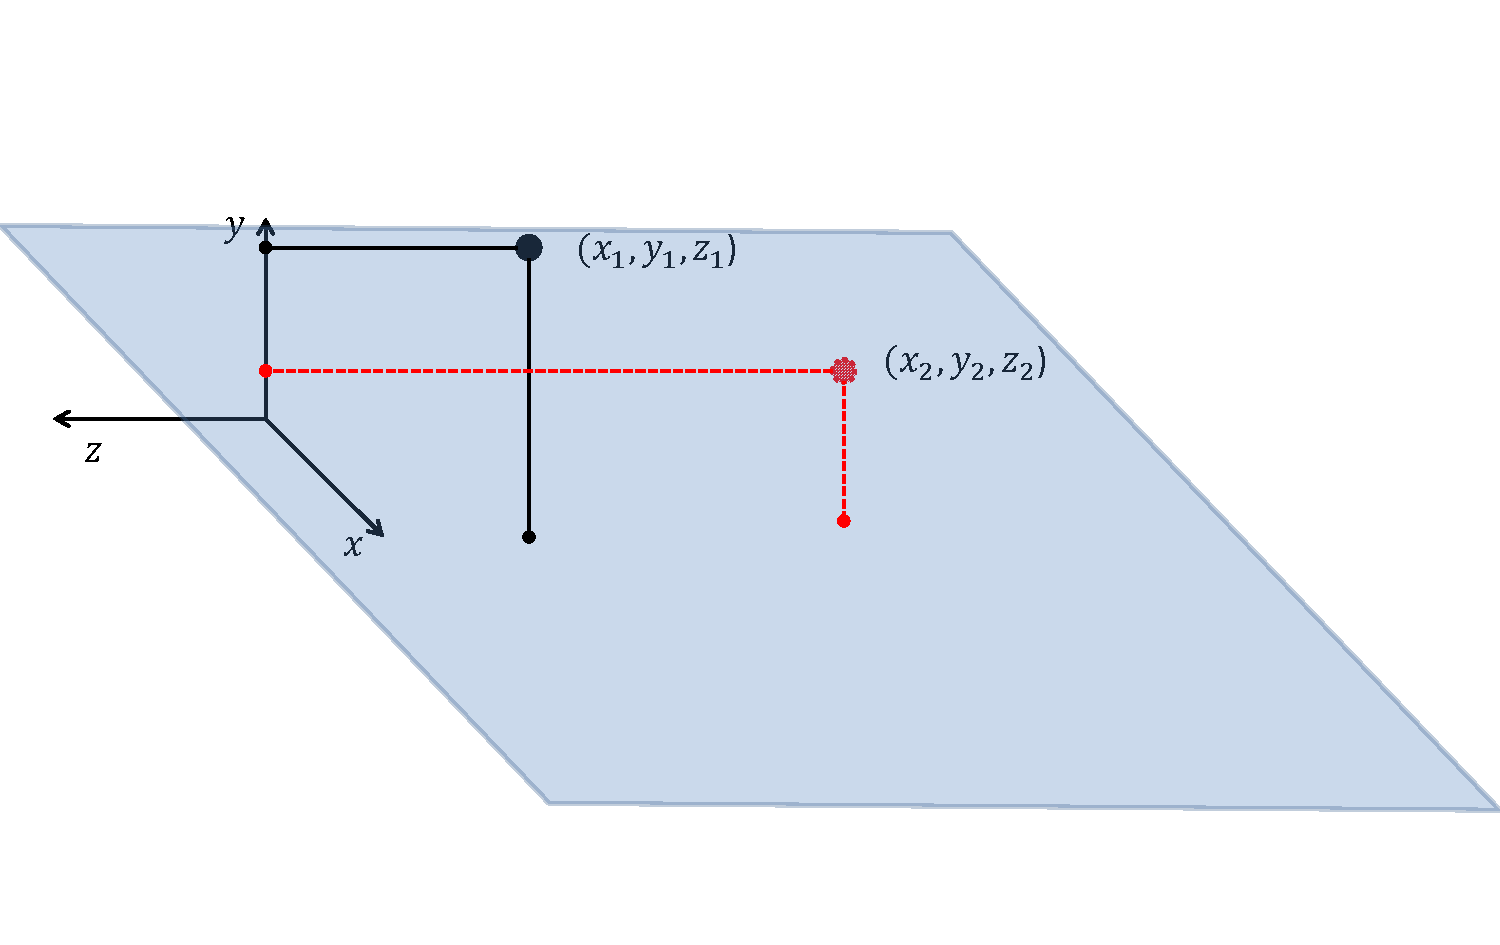
\includegraphics[width=0.85\textwidth]{Wakefields_and_Impedances/figures/source-witness-pos.pdf}
\end{center}
\caption{The relative displacements and velocities of the source and test particles.}
\label{fig:source_and_wit}
\end{figure} 

\subsection{The Electromagnetic Fields of a Moving Charged Particle in Free Space}

If we consider the electromagnetic fields generated by the source particle, it can be shown that the fields at a vector $\mathbf{R} = \mathbf{r_{1}} - \mathbf{r_{2}}$ is given by

\begin{align}
\mathbf{E}\left( \mathbf{R}  \right) = \frac{q_{1}\mathbf{R}}{\gamma^{2}\left| \mathbf{R} \right|^{3}} \\
\mathbf{H}\left( \mathbf{R}  \right) = \frac{1}{c}\mathbf{v} \times \mathbf{E}
\label{eqn:gen_fields_mov_part}
\end{align}

where $\gamma = \sqrt{1- v^{2}/c^{2}}$ is the relativistic gamma factor. It can be shown that, if we take the ultrarelativistic limit (i.e. $\gamma \rightarrow \infty$) we can see that Eqn~\ref{eqn:gen_fields_mov_part} becomes

\begin{equation}
\mathbf{E}\left( \mathbf{R}  \right) = \frac{2q_{1}\mathbf{r}}{r^{3}}\delta{z-ct} \\
\mathbf{H}\left( \mathbf{R}  \right) = \mathbf{\hat{z}} \times \mathbf{E}
\label{eqn:ultrarel_field_eqn}
\end{equation}

where $\mathbf{r} = x\mathbf{\hat{x}} + y\mathbf{\hat{y}}$ is a purely transverse vector.

The following witness particle this experiences the resulting lorentz force 

\begin{equation}
\mathbf{F}\left(\mathbf{r_{1}}, \mathbf{r_{2}}  \right) = q_{2}\left[ \mathbf{E} + \mathbf{v} \times \mathbf{B}  \right]. 
\end{equation}

Looking at Eqn.~\ref{eqn:ultrarel_field_eqn}, it can be seen that the force can be seperated into longitudinal and transverse components 

\begin{align}
F_{\parallel}\left(\mathbf{r_{1}} \mathbf{r_{2}}  \right) = q_{2}E_{\parallel} \\
\mathbf{F_{\perp}}\left(\mathbf{r_{1}}, \mathbf{r_{2}}  \right)  = q_{2}\left[ \mathbf{E_{\perp}} + \mathbf{v} \times \mathbf{B} \right]
\end{align}

where $E_{\parallel} = \mathbf{E}.\mathbf{\hat{z}}$ and $\mathbf{E_{\perp}} = E_{x}\mathbf{\hat{x}} + E_{y}\mathbf{\hat{y}}$. $F_{\parallel}$ has only an electric component as the magnetic flux density $\mathbf{B}$ has magnitude = 0 in the $\mathbf{\hat{z}}$ direction. Considering just the longitudinal force, integrating over all space gives the total energy change of the source particle

\begin{equation}
U_{1}\left(\mathbf{r_{1}}  \right) = -q_{2} \int^{\infty}_{-\infty} d\mathbf{z} . \mathbf{F}\left(\mathbf{r_{1}}, \mathbf{r_{2}}  \right),
\end{equation}

where $t = z_{1}/\beta{}c = z_{1}/c$ in the ultrarelativistic case. Similarly the energy change in the witness particle can be calculated by

\begin{equation}
U_{2}\left(\mathbf{r_{1}}, \mathbf{r_{2}}, \tau  \right)  = -q_{2} \int^{\infty}_{-\infty} d\mathbf{z} \mathbf{F}\left(\mathbf{r_{1}}, \mathbf{r_{2}}  \right),
\label{eqn:witness_energy_change_single}
\end{equation}

where $t = z_{1}/\beta{}c = z_{1}/c + \tau$ and $\tau = \left( z_{1}-z_{2} \right)/\beta{}c$ is the time between the source and witness particle. From these two energy losses two widely used terms can be extracted; the loss factor $k$, given by

\begin{equation}
k\left(\mathbf{r_{1}}  \right) = \frac{U_{1}\left(\mathbf{r_{1}}  \right)}{q_{1}}
\end{equation}

and the longitudinal wake function, given by

\begin{equation}
w_{\parallel}\left(\mathbf{r_{1}}, \mathbf{r_{2}}, \tau   \right) = \frac{U_{2}\left(\mathbf{r_{1}}, \mathbf{r_{2}}, \tau  \right) }{q_{1} q_{2}},
\label{eqn:long_wake_func}
\end{equation}

denoting the normalised (with respect to source charge, and source and witness charge respectively) energy change of both the source particle (loss factor) and witness particle (wake function). 

\subsection{Wakefields of a Bunch}

As colliders are often used to collide bunches of particles as opposed to single particles, it is useful to be able to define the wake function of a bunch distribution. It can be seen that the total source charge of a bunch $q_{1}$ is the integral of the longitudinal current distribution $i_{b}\left( \tau \right)$ integrated over all time

\begin{equation}
q_{1} = \int^{\infty}_{-\infty}i_{b}\left( \tau \right) d\tau{}.
\end{equation}

The wake function of a bunch distribution at a point at time $\tau$ can be calculated by the convolution of the single particle wake function with the bunch distribution. Thus, if the bunch is split into infinitesimally small slices, the change in energy of a witness particle of charge $q$ at time $\tau$ due to a slice at time $\tau{}'$ is given by

\begin{equation}
dU\left(\mathbf{r_{2}}, \tau-\tau{}'  \right) = q i_{b}\left( \tau{}' \right) w_{\parallel}\left( r_{2}, \tau{}-\tau{}' \right).
\end{equation}

The longitudinal bunch wake function $W_{\parallel}\left(\mathbf{r_{2}}\right)$ can then be calculated using Eqn.~\ref{eqn:witness_energy_change_single}

\begin{equation}
W_{\parallel}\left( \mathbf{r_{2}}, \tau \right) = \frac{U\left( r_{2}, \tau \right) }{q_{1} q_{2}} = \frac{1}{q_{1}}\int^{\infty}_{-\infty}i_{b}\left( \tau{}' \right) w_{\parallel}\left( r_{2}, \tau{}-\tau{}'\right) d\tau{}' .
\end{equation}

\subsection{Transverse Wakefields}

Similar to the longitudinal wakefield, we can see that the total tranverse momentum change of the witness particle is given by integrating the transverse force across all space

\begin{equation}
\mathbf{P}\left(\mathbf{r_{1}}, \mathbf{r_{2}}, \tau  \right) = \int^{\infty}_{-\infty} \mathbf{F_{\perp}} \left( \mathbf{r_{1}} \mathbf{r_{2}}\right) dz
\end{equation}

where $t = z_{1}/c + \tau$ and again $\tau$ is the time delay between source and witness particles. And similarly to the longitudinal plane we can define a wake function normalised with regards to the source and witness particle charges

\begin{equation}
\mathbf{w_{\perp}}\left(\mathbf{r_{1}}, \mathbf{r_{2}}, \tau  \right) = \frac{\mathbf{P}\left(\mathbf{r_{1}}, \mathbf{r_{2}}, \tau  \right)}{q_{1} q_{2}}.
\label{eqn:trans_wake_func}
\end{equation}

And in a similar manner to the longitudinal bunch wake function a form for the transverse bunch wake function can be derived

\begin{equation}
W_{\perp}\left( \mathbf{r_{2}}, \tau \right) = \frac{U\left( r_{2}, \tau \right) }{q_{1} q_{2}} = \frac{1}{q_{1}}\int^{\infty}_{-\infty}i_{b}\left( \tau{}' \right) w_{\perp}\left( r_{2}, \tau{}-\tau{}'\right) d\tau{}' .
\end{equation}

\subsection{Panowsky-Wenzel Theorem}

Considering the force acting on the witness particle it can be seen to simply by the Lorentz force

\begin{equation}
\mathbf{F} = q_{2} \left[\mathbf{E} + \mathbf{v}\times \mathbf{B} \right]
\label{eqn:wit_gen_force}
\end{equation}

Now, considering Faraday's law in integral form ($\mathbf{B} = -\int^{t_{2}}_{t_{1}} \left( \nabla \times \mathbf{E} \right) dt$, $t_{1}$ being sufficiently in the past that $\nabla \times \mathbf{E} \rightarrow 0$), Eqn.~\ref{eqn:wit_gen_force} can be rewritten as

\begin{equation}
\mathbf{F} = q_{2}  \left[\mathbf{E} - \mathbf{v}\times\left(  \int^{t_{2}}_{t_{1}} \nabla \times \mathbf{E} dt \right) \right].
\end{equation}

Now, using the fact that the velocity $\mathbf{v}$ is constant and some vector identities this then becomes

\begin{equation}
\mathbf{F} = q_{2}  \left[\mathbf{E} - \int^{t_{2}}_{t_{1}}\left(  \nabla \left( \mathbf{v} . \mathbf{E} \right)  - \mathbf{v}\left( \nabla . \mathbf{E} \right) \right) dt  \right].
\end{equation}

If this force is seperated into the longitudinal and transverse components we see that they are the following

\begin{align}
F_{\parallel} = q_{2} E_{z} \\
\mathbf{F}_{\perp} = q_{2}  \left[\mathbf{E_{\perp}} - v \int^{t_{2}}_{t_{1}}\left(  \nabla_{\perp}E_{z}  - \frac{\partial\mathbf{E}_{\perp}}{\partial z} \right) dt  \right]
\end{align}

where $\nabla_{\perp}$ in the differential operator only in the transverse coordinates. If these are now compared to the identities of the wake function for the longitudinal and transverse wake functions given in Eqns.~\ref{eqn:long_wake_func; eqn:trans_wake_func} respectively, it can be seen that

\begin{align}
w_{\parallel}\left( \mathbf{r_{1}}, \mathbf{r_{2}}, \tau   \right) = -\frac{1}{q_{1}} \int^{\infty}_{-\infty} dz E_{z} \left( \mathbf{r_{1}}, \mathbf{r_{2}} \right) \\
\mathbf{w}_{\perp} \left(\mathbf{r_{1}}, \mathbf{r_{2}}, \tau   \right) = \frac{1}{q_{1}} \int^{\infty}_{-\infty} dz \left[ \mathbf{E_{\perp}}\left(\mathbf{r_{1}}, \mathbf{r_{2}} \right) - v   \int^{t_{2}}_{t_{1}}\left(  \nabla_{\perp}E_{z}\left(\mathbf{r_{1}}, \mathbf{r_{2}} \right)  - \frac{\partial\mathbf{E}_{\perp}\left(\mathbf{r_{1}}, \mathbf{r_{2}} \right)}{\partial z} \right) dt \right] \label{eqn:trans_wake_middle}.
\end{align}

The next stage requires partially differentiating Eqn~\ref{eqn:trans_wake_middle} by $s = v \tau = vt - z$. It can be seen from this relationship that $\partial / \partial s = - \partial / \partial z$ and $\partial / \partial s = 1/v \partial / \partial z$. Thus the first term can be replaced by $\partial / \partial s = - \partial / \partial s$, and the term the integral becomes the value of the intergrand at $\tau$.

\begin{equation}
\frac{\partial}{\partial s}\mathbf{w}_{\perp} \left(\mathbf{r_{1}}, \mathbf{r_{2}}, \tau   \right) = \frac{1}{q_{1}} \int^{\infty}_{-\infty} dz \left[ \frac{-\partial}{\partial z}\mathbf{E_{\perp}} - \left(  \nabla_{\perp}E_{z} + \frac{\partial\mathbf{E}_{\perp}}{\partial z} \right) dt \right].
\end{equation} 

It can be seen that the first and third integrand cancel. Also, the operator $\nabla_{\perp}$ may be moved to the front of the operation without changing the equation, thus

\begin{equation}
\frac{\partial}{\partial s}\mathbf{w}_{\perp} \left(\mathbf{r_{1}}, \mathbf{r_{2}}, \tau   \right) =  \frac{1}{q_{1}} \int^{\infty}_{-\infty} dz \nabla_{\perp}E_{z} = \mathbf{\nabla_{\perp}} w_{\parallel}\left( \mathbf{r_{1}}, \mathbf{r_{2}}, \tau   \right).
\end{equation}

%\begin{itemize}
%\item{Introduction to the electromagnetic field of charged particle moving in free space}
%\item{Field of a particle in a perfectly conducting pipe - method of image currents}
%\item{Place a witness particle distance s behind source particle and deduce electric field as seen by this particle}
%\item{normalise this by the source particle charge to give the wakepotential}
%\item{And again by the source particle charge and current profile to acquire the loss factor}
%\item{Longitudinal field predominantly}
%\item{Introduce the Panowsky-Wenzel theorem covering transverse field - Transverse wakes}
%\end{itemize}

\section{Impedances}

In a particle accelerator there are a large number of components that have frequency dependent properties, either due to their geometry (for example resonant cavity structures) or material properties (frequency dependent permitivitty/permeability in devices, for example ferrite in normal conducting kicker magnets). In addition many instability mechanisms are strongly modal in nature, thus a frequency analysis of the possible sources of impedance is incredibly valuable. 

\subsection{Beam Coupling Impedance}

The longitudinal beam coupling impedance $Z_{\parallel}$ and the transverse beam coupling impedance $Z_{\perp}$ are defined as the Fourier transforms of the single particle wake function, given by

\begin{align}
Z_{\parallel} \left(\mathbf{r_{1}}, \mathbf{r_{2}}, \omega  \right) = \int^{\infty}_{0} d\tau w_{\parallel} \left(\mathbf{r_{1}}, \mathbf{r_{2}}, \tau  \right) e^{-j\omega \tau}\\
Z_{\perp} \left(\mathbf{r_{1}}, \mathbf{r_{2}}, \omega  \right) = j \int^{\infty}_{0} d\tau w_{\perp} \left(\mathbf{r_{1}}, \mathbf{r_{2}}, \tau  \right) e^{-j\omega \tau} \label{eqn:total_trans_imp}
\end{align}

where. In a similar way the bunch wake function (often called the wake potential) can be related to the longitudinal and transverse beam coupling impedance by considering the Fourier transform of the time dependent bunch current $\lambda \left( \omega  \right) = \int^{\infty}_{-\infty} d\tau i_{b}\left( \tau \right) e^{-j \omega \tau}$, which allows it to be shown that

\begin{align}
W_{\parallel}  \left( \mathbf{r_{2}}, \tau \right) = \int^{\infty}_{- \infty} d \omega Z_{\parallel} \left(\mathbf{r_{1}}, \mathbf{r_{2}}, \omega  \right) \lambda \left( \omega  \right) e^{j \omega \tau} \\
W_{\perp}  \left( \mathbf{r_{2}}, \tau \right) = \int^{\infty}_{- \infty} d \omega Z_{\perp} \left(\mathbf{r_{1}}, \mathbf{r_{2}}, \omega  \right) \lambda \left( \omega  \right) e^{j \omega \tau}.
\end{align}

\subsection{Transverse Impedances}

As can be seen in Eqn.~\ref{eqn:total_trans_imp}, the transverse impedance is dependent on the displacement of both the source and witness particles. To evaluate the beam dynamics to only the first order (i.e. only small perturbations in $x$ and $y$ are considered allowing the use of perturbation theory. Coupling terms between $x,y$ are then second order effects and maybe ignored), it is useful to distinguish the components dependent only on the transverse displacement of the source particle and that of the witness particle in the vertical and horizontal planes of the beam. This involves seperating the impedance firstly into horizontal and vertical components, and subsequently into components dependent only on the displacement of the source and of the witness particle. These are called the dipolar, or driving impedance and the quadrupolar, or detuning impedance respectively. In addition it can be shown that constant transverse terms exist in asymmetric structures which should also be taken into account. These are given by

\begin{align}
Z_{\perp, x} \left( x_{1}, x_{2}, \omega \right) &= Z_{dip, x} \left( \omega  \right) x_{1} +  Z_{quad, x} \left( \omega   \right)x_{2} + Z_{const, x} \left( \omega  \right) \\
Z_{\perp, y} \left( y_{1}, y_{2}, \omega \right) &= Z_{dip, y} \left( \omega  \right)y_{1} +  Z_{quad, y} \left( \omega \right)y_{2} + Z_{const, y} \left( \omega  \right).
\end{align}

The relative displacements of the source and witness particles are shown in Fig.~\ref{fig:trans_imp_disp} for clarity.

\begin{figure}
\begin{center}
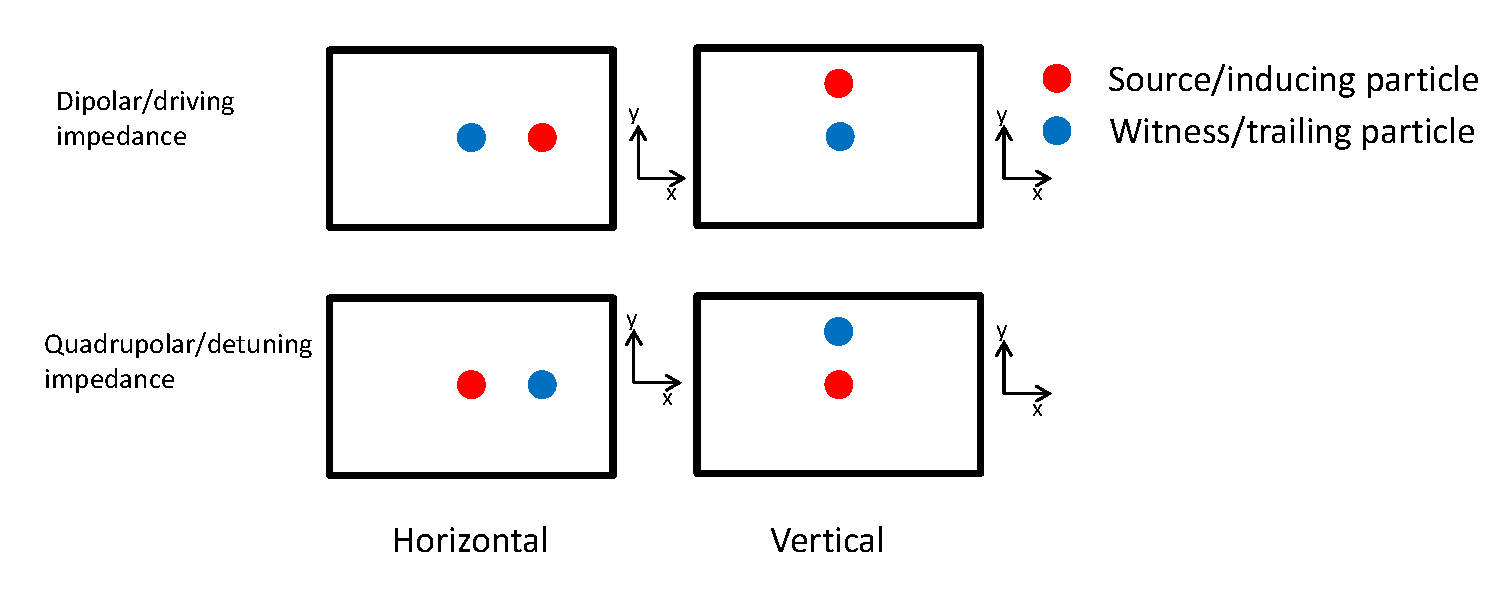
\includegraphics[width=0.9\textwidth]{Wakefields_and_Impedances/figures/impedance-des.pdf}
\end{center}
\caption{The relative displacements of the source particle and witness particle in the horizontal and vertical planes that identify the dipolar/driving and quadrupolar/detuning impedances.}
\label{fig:trans_imp_disp}
\end{figure}

%\begin{itemize}
%\item{Firstly mention the commonality of frequency dependent material properties - ferrite permeability, permitivitty determined by conductivity/frequency in conductors/dielectrics/skin depth}
%\item{Fourier transform of wakefield into the convolution of the beam current spectrum and the impedance}
%\item{Again Panowsky-Wenzel for impedance}
%\item{Discussion of the transverse impedance - in particular the general definition of an impedance (n-th order current interacting with an m-th order field)}
%\item{Define dipolar/driving and quadrupolar/detuning impedance. In addition constant transverse impedance term}
%\end{itemize}
\subsection{Geometric Impedance}
\label{sec:imp_geo_imp}

Geometric impedances are characterised by resonant fields at a resonant frequency, typically attributable to some characteristic dimension of the structure; for example a length of a structure (cavity size, antenna length), which may be part of a vacuum tank, or an internal structure to the device exhibiting the resonance. 

As a simple example, consider a cylindrical pillbox cavity of radius $r_{cav}$ and length $L$ connected to a beam pipe of radius $r_{pipe}$ located at the centre of the cavity, as shown in Fig.~\ref{fig:cylin_geo_diagram}. For simplicity we shall assume that the cavity is made from a perfectly conducting material. It shall be assumed that the fields do not propogate along the attached beam pipe (i.e. for frequencies below beam pipe cutoff). In this example we shall consider a particle travelling on the axis of the beam pipe, and only the longitudinal wakefunction/impedance will be investigated to simplify matters. Further details can be found in \cite{Wolsky:TheoryEM, Jensen:RFCav, Stupakov:wakeAndImp}. It can be shown that there are two families of resonant modes in in a pillbox cavity, TM-type modes and TE-type modes. The TE-type modes have no longitudinal electrical field by definition, and therefore do not contribute to the longitudinal wakefunction for an on axis particle. In a cylindrical coordinate system using coordinates $(r, \theta, z)$, the longitudinal electrical field of the $n$-th order TM-type modes can be shown to be

\begin{equation}
E_{z,n} = E_{0}J_{n}\left( k_{r} r \right) cos \left( n \theta \right) cos \left( k_{z} z \right) e^{-j \omega t}
\end{equation}

where $E_{0}$ is the magnitude of the electric field, $J_{n}$ is $n$-th order Bessel function, $k_{z}=n\pi{}/L$, and $n$ is an interger. A wakefunction for each mode can subsequently be defined as $w_{\parallel ,n}\left(( \mathbf{r}_{1}, \mathbf{r}_{2}, \tau \right)$, where the total wakefunction is thus defined as

\begin{equation}
w_{\parallel} \left( \mathbf{r}_{1}, \mathbf{r}_{2}, \tau \right) =  \displaystyle\sum\limits_{n = 0}^{\infty} w_{\parallel ,n} \left(( \mathbf{r}_{1}, \mathbf{r}_{2}, \tau \right) = \frac{-1}{q_{1}}\displaystyle\sum\limits_{n = 0}^{\infty} \int^{\infty}_{-\infty} dz E_{z,n} \left( r, \theta , z \right)
\end{equation}

\begin{figure}
\begin{center}
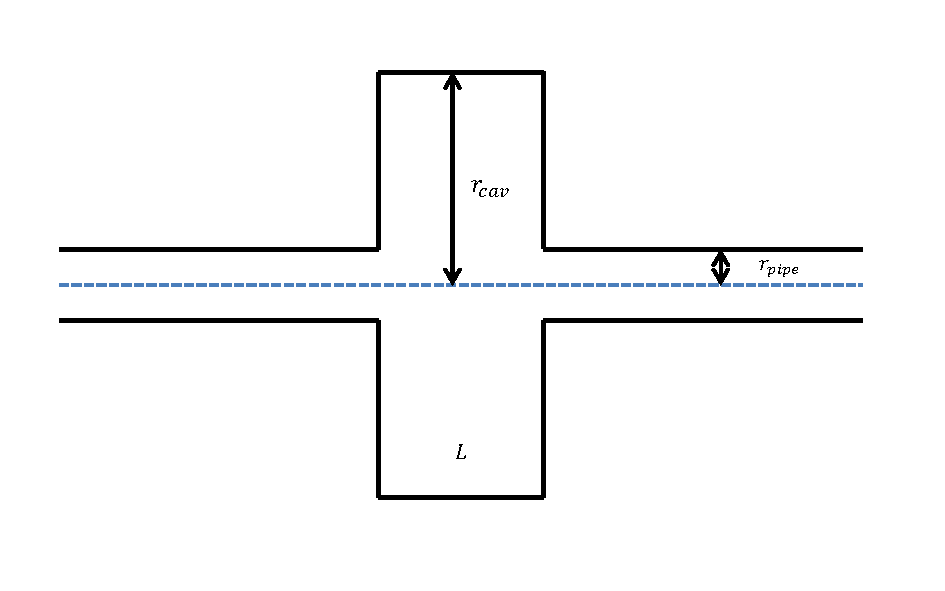
\includegraphics[width=0.7\textwidth]{Wakefields_and_Impedances/figures/pillbox-cav.pdf}
\end{center}
\caption{Cross section of a cylindrical pillbox cavity with an attached beam pipe.}
\label{fig:cylin_geo_diagram}
\end{figure}

To evaluate the problem in the frequency domain we shall introduce the RLC parallel circuit model to simplify the frequency doman representation.

\subsubsection{RLC Circuit Model}

We can define any given resonance by an equivalent RLC circuit, which is driven by a current $i_{b}$, shown in Fig.~\ref{fig:rlc_circ}. The symbols represent the equivalent resistance ($R_{s}$), inductance ($L$) and capcitance ($C$). From this circuit a number of defining parameters are now deduced, and the physical equivalents in the actual cavity are described.

\begin{figure}
\begin{center}
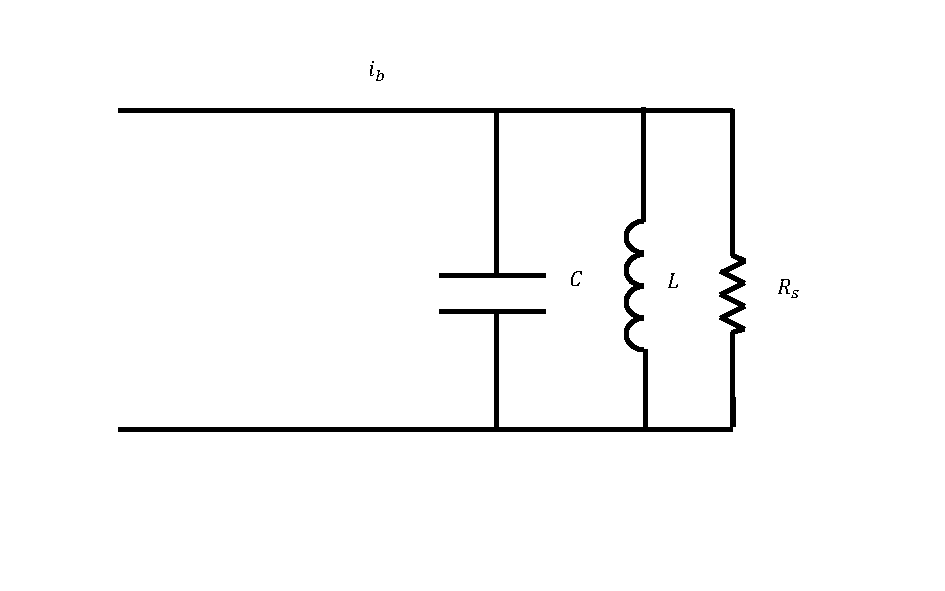
\includegraphics[width=0.7\textwidth]{Wakefields_and_Impedances/figures/equiv-circuit.pdf}
\end{center}
\caption{The equivalent RLC parallel circuit for a cavity resonance, driven by a current $i_{b}$, in this case the beam current.}
\label{fig:rlc_circ}
\end{figure}

The first parameter to be derived is the resonant frequency of the cavity mode itself $\omega_{res}$. This can be shown (by solving the time varying voltage build up of the circuit in Fig.~\ref{fig:rlc_circ}) to be given by

\begin{equation}
\omega_{res} = \frac{1}{\sqrt{LC}}.
\end{equation}

Next we define the quality factor of the $n$-th cavity mode, $Q_{n}$. This factor describes the damping of the wakefunction in the cavity for a given mode, larger values indicating a longer damping time. In terms of the cavity it is given by

\begin{equation}
Q_{n} = \frac{\omega_{res} W}{P_{surf}} = \omega_{0}R_{s}C
\end{equation}

where $W = \int_{V} \frac{\epsilon}{2} \left| \mathbf{E} \right|^{2} dV$ is the time-averaged stored electromagnetic energy in the cavity due to the mode (sometimes given as $U$), $\epsilon = \epsilon_{r}\epsilon_{0}$ is the permitivitty, $\epsilon_{r}$ the relative permitivitty, $\epsilon_{0}$ the permitivitty of free space and $P_{surf}$ is the total losses in the cavity. Commonly the latter is dominated by conductive losses on the cavity walls, but as will be seen in later sections, also includes losses due to other mechanisms. The final figures of merit are the $R_{s, n}/Q_{n}$ of the cavity mode, and the shunt impedance $R_{s, n}$ of the mode. $R_{s, n}/Q_{n}$ is given by

\begin{equation}
\frac{R_{s, n}}{Q_{n}} = \frac{\left| V_{acc} \right|^{2}}{2 \omega_{res} W}
\end{equation}

where $V_{acc} = \int^{\infty}_{-\infty} E_{z, n} e^{-j \omega_{res} z/ \beta{}c} dz$ is the effective voltage that a traversing particle sees due to the cavity mode. It can thus be seen that the $R_{s, n}/Q_{n}$ of a cavity mode gives some ratio of the acceleration of a traversing particle to the stored energy. The shunt impedance $R_{s, n}$ is then given by

\begin{equation}
R_{s, n} = \left(  \frac{R_{s, n}}{Q_{n}} \right) Q_{n} = \frac{\left| V_{acc} \right|^{2}}{2 P_{surf}}
\end{equation}

or an equivalent ratio for power loss in the cavity to acceleration of the particle. From these quality factors is defined a broadband description of the beam coupling impedance at all frequencies due to all modes, given by

\begin{equation}
Z_{\parallel} \left( \omega \right) = \displaystyle\sum\limits_{n = 0}^{\infty} Z_{\parallel, n} \left( \omega \right) = \displaystyle\sum\limits_{n = 0}^{\infty} \frac{R_{s, n}}{1 - jQ \left( \frac{\omega}{\omega_{res}} - \frac{\omega_{res}}{\omega} \right)}.
\end{equation}

A number of examples of this type of impedance are shown in Sec.~\ref{sec:beam_induced_heating}.
\subsection{Resistive Wall Impedance}
\label{sec:res_wall_imp}

The resistive wall impedance is an impedance generated due to the finite conductivity of the material of the beam pipe wall. This can have a number of regimes dependent on whether the skin depth of the material $\delta \left( \omega \right) = \sqrt{\frac{2}{\mu_{0} \mu_{r} \sigma \omega}}$ ($\mu_{0}$ being the permeability of free space, $\mu_{r}$ the relative permeability of the material, $\sigma$ the conductivity of the wall material) is much smaller than the thickness of the beam pipe wall \cite{Chao:PhysColEff}, comparable to the thickness of the beam pipe wall \cite{Roncarolo:ColImpMeas, Metral:ResWallWideFreq} or much larger than the thickness of the beam pipe wall \cite{Tsutsui:ferrKickLong, Biancacci:MMFiniteInsert}, in addition to the pipe radius and the thickness of the pipe wall (such as the case of an a pipe wall of infinite thickness). In this instance, $\sigma$ is the conductivity of wall material. It can also be shown that the shape of the beam pipe cross section also plays a significant role in defining the impedance \cite{Mounet:Axisymmetric, Mounet:Flat}.

Here we shall not attempt a comprehensive summary of the various resistive wall impedance models, but simply give an example of a model in the form of the Tsutsui formalism to give a sense of how changing the wall conductivity affects the resistive wall impedance. A considerably more detailed overview of this derivation can be found in App.~\ref{app:analyticalMods} \cite{Tsutsui:ferrKickLong, Tsutsui:DipoleKicker}. Consider two parallel plates of a resistive material, as shown in Fig.~\ref{fig:res_wall_diagram}, between which moves a source particle of charge $q_{1}$ moving with velocity $\mathbf{v} = \beta c \mathbf{\hat{z}}$. In this case it shall be assumed that $\beta = 1$.

\begin{figure}
\begin{center}
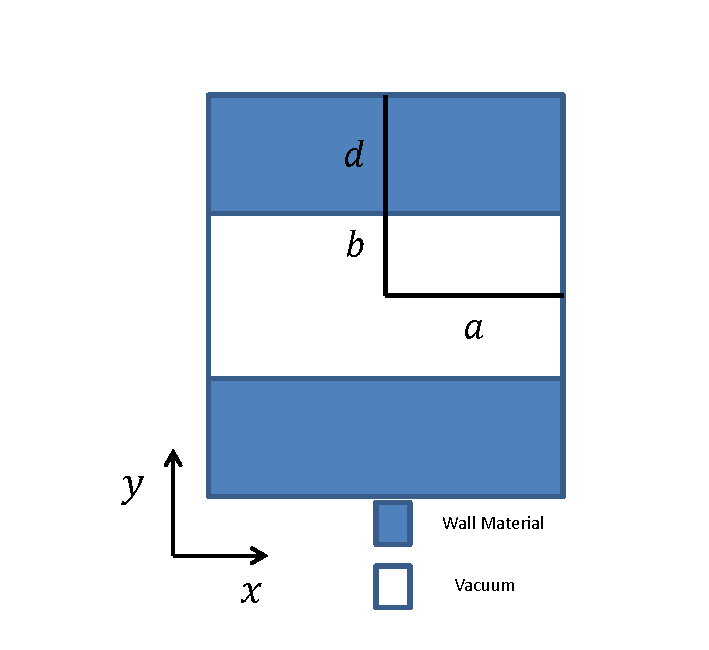
\includegraphics[width=0.6\textwidth]{Wakefields_and_Impedances/figures/reWallGeo.pdf}
\end{center}
\caption{The geometry of the Tsutsui resistive wall formalism.}
\label{fig:res_wall_diagram}
\end{figure}

The longitudinal and dipolar impedances for this model can be seen in Fig.~\ref{fig:resWallImpComp} for a comparison between two sample materials. It can be seen that for the given frequency range there are two regimes for both the longitudinal and transverse impedance (although the difference is more pronounced for the transverse impedance). For high frequencies, the classical thick wall formalism (as in \cite{Chao:PhysColEff}) applies, as the skin depth of the material is much smaller than the beam pipe aperture and the layer's thickness. Susequently this formalism would predict a greater impedance at lower frequencies, as it gives $Z_{\perp} \propto \omega^{-1/2}$. At lower frequencies however this is not seen to be the case. This is due to the following reasons:

\begin{enumerate}
\item{At high frequencies the beam induced current effectively flows on the surface of the material, thus the distance between the beam image current and the witness particle is constant at value $b$. Thus the transverse impedance seen is determined by the change in skin depth $\delta$ which is proportional to $\omega^{-1/2}$}
\item{At low frequencies the beam image current effectively flows some distance inside the wall material, greater than $b$. This increases the distance between the beam image current and the witness particle, thus decreases the force seen by the witness particle. This causes the transverse impedance to become linear with respect to $\omega$. It is important to note this mechanism, as it indicates that this phenomena occurs at a "low" frequency for any thickness of wall material, even for a wall of infinite thickness.}
\item{The transition region occurs when these two phenomena become of similar magnitude. The frequency at which the real component of the transverse impedance reaches it's maximum can be shown to be proportional to $1/(\sigma b^{2})$.}
\end{enumerate}

\begin{figure}
\subfigure[]{
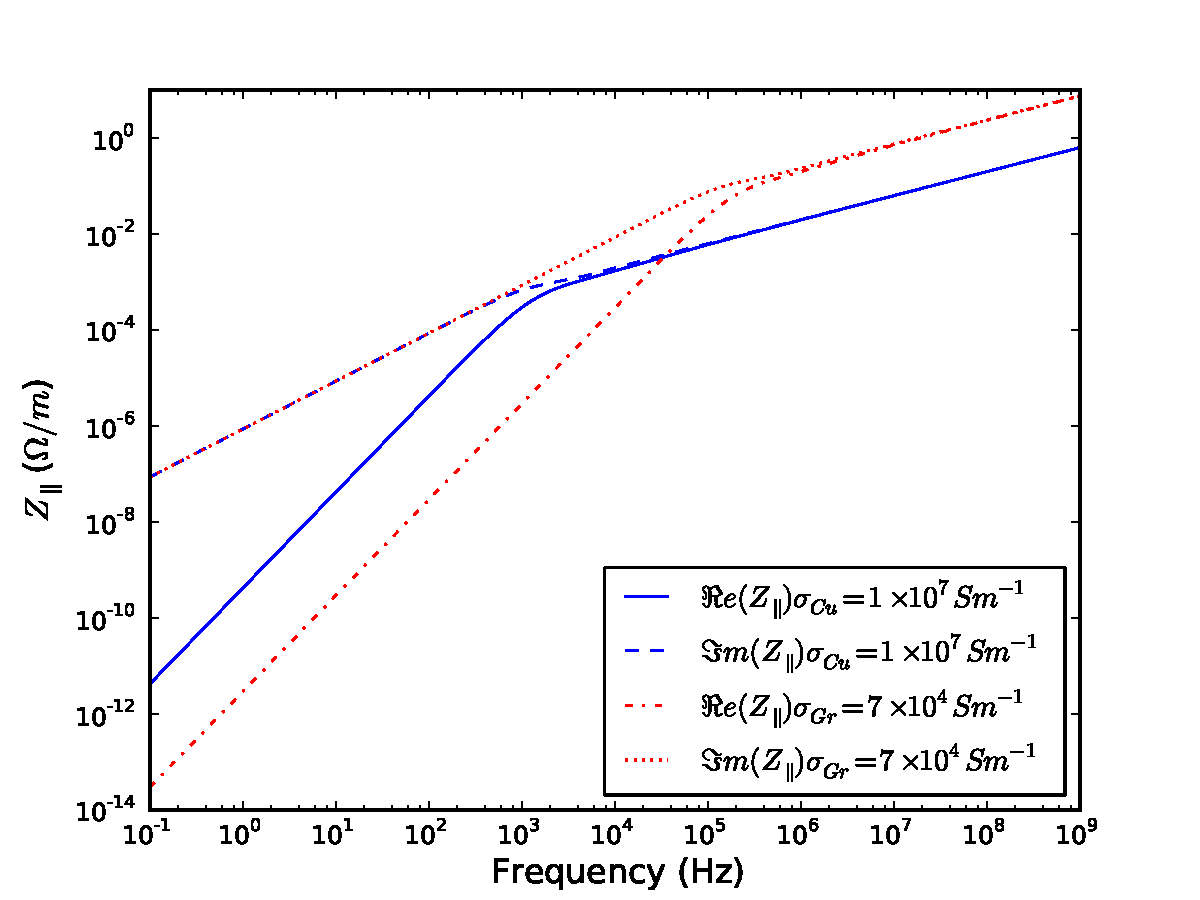
\includegraphics[width=0.5\textwidth]{Wakefields_and_Impedances/figures/resWallTsutsuiLong.pdf}
\label{fig:reswalllong}
}
\subfigure[]{
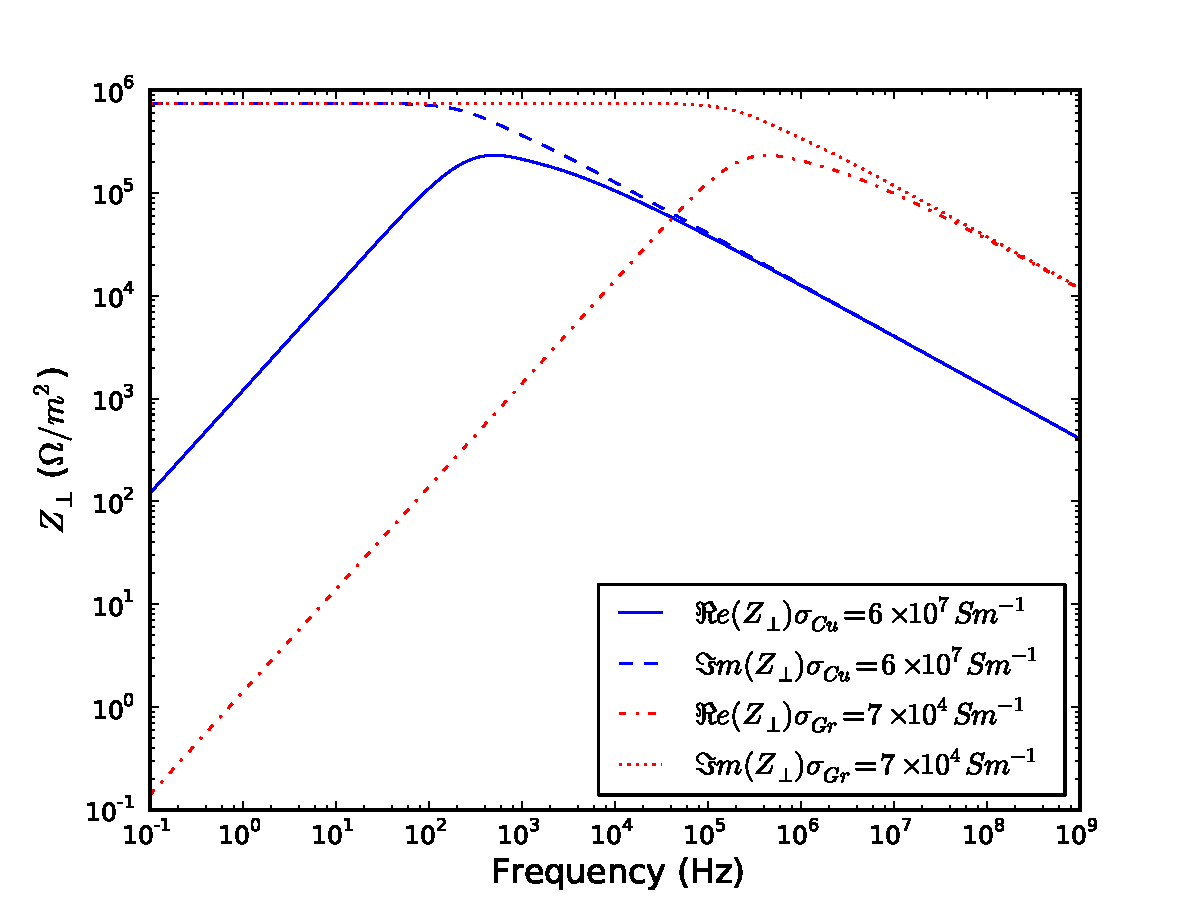
\includegraphics[width=0.5\textwidth]{Wakefields_and_Impedances/figures/resWallTsutsuiTrans.pdf}
\label{fig:reswalltrans}
}

\caption{Examples of the longitudinal \subref{fig:reswalllong} and transverse \subref{fig:reswalltrans} resistive wall impedance per unit length of a beam pipe of aperture $a = 2cm$ made of both copper ($\sigma = 6 \times 10^{7} S m^{-1}$) and graphite ($\sigma = 7 \times 10^{4} S m^{-1}$).}
\label{fig:resWallImpComp}
\end{figure}


\section{Example of the Effects of Wakefields}

To give context to the effects that wakefields have on both the beam and equipment within a particle accelerator, two types of wakefield/impedance driven phenomena are discussed here. The first, beam-induced heating, is an example of beam induced wakefields having an effect on the machine itself contributing to heat loads due to the energy lost by the beam and subsequently dissipated within the surrounding equipment. The second, beam instabilities, covers a number of examples of instability mechanisms that may be driven by wakefields, in particular due to the harmonic nature of particle and beam behaviour in a circular accelerator.

\subsection{Beam Induced Heating}
\label{sec:beam_induced_heating}

\subsubsection{Defining and Deriving Power Loss in Circular Accelerators}
\label{sec:power_loss}

When a charged particle interacts with a wakefield it's energy changes due to the field that it sees. Assuming a beam with a longitudinal distribution $\rho (\tau)$, normalised such that $\int d \tau \rho (\tau ) = I_{b}$. Now a normalised longitudinal distribution $\rho_{n}$ is introduced, such that $\rho = N_{b} f_{rev} e \int d \tau \rho_{n}$. Thus the energy change of the distribution $\rho$ traversing a pipe for a distance $L$ is given by \cite{Chao:PhysColEff, Ng:IntDepInstab}

\begin{equation}
\Delta E = - \left( f_{rev} e N_{b}\right)^{2} \int^{\infty}_{-\infty} d\tau^{'} \rho_{n} \left( \tau^{'} \right) \int^{\infty}_{-\infty} d\tau^{} \rho_{n} \left( \tau^{} \right) W_{\parallel} \left( \tau^{'} - \tau \right).  
\end{equation}

Written in terms of the Fourier transformed quantities this becomes

\begin{equation}
\Delta E = \frac{-1}{2\pi}\left( f_{rev} e N_{b}\right)^{2} \int^{\infty}_{-\infty} d\omega \left| \lambda \left( \omega \right)  \right|^{2} \Re{}e \left[ Z_{\parallel} \left( \omega \right) \right]
\end{equation}

where 

\begin{equation}
\lambda \left( \omega \right) = \frac{1}{\sqrt{2 \pi}}\int^{\infty}_{-\infty} d \tau \rho_{n} \left( \tau \right) e^{j\omega \tau}. 
\end{equation}

For a mode expansion representation of the wakefunction as a sum of loss factors, the total energy change can be written as 

\begin{equation}
\Delta E = \left( f_{rev} e N_{b}\right)^{2} \displaystyle\sum\limits_{n = 0}^{\infty} k_{n} \left| \lambda \left( \omega_{n} \right)  \right|^{2}.
\end{equation}

These terms are valid only for a single pass of the beam through the impedance (i.e. for a linear accelerator). In the case where the beam traverse the same impedance multiple times (i.e. a circular accelerator) it is necessary to take into account the wakefields induced by previous traversals. In this case the energy lost by the beam due to traversing the pipe is given by

\begin{equation}
\Delta E = - \left( f_{rev} e N_{b}\right)^{2} \int^{\infty}_{-\infty} d\tau^{'} \rho_{n} \left( \tau^{'} \right) \int^{\infty}_{-\infty} d\tau^{} \rho_{n} \left( \tau^{} \right) \displaystyle\sum\limits_{q = 0}^{\infty} W_{\parallel, q} \left( q\frac{C}{c} + \tau^{'} - \tau \right)  
\label{eqn:sum_wake_loss}
\end{equation}

where $C$ is the circumference and $q$ sums over revolutions. In general impedance is the more useful property to use compared to wakefields. Using the Poisson sum formalism and the following identity

\begin{equation}
\displaystyle\sum\limits_{n = -\infty}^{\infty} F \left( n a \right) = \frac{1}{a} \displaystyle\sum\limits_{p = -\infty}^{\infty} \tilde{F} \left( \frac{2\pi p}{a} \right)
\end{equation}

where $F(\tau)$ and $\tilde{F}(\omega)$ are arbitary Fourier transformed pairs. This relationsgip shows that summing a function at regular intervals $a$ is equal to summing over its Fourier transformed counterpart at regular intervals $\frac{2 \pi}{a}$. In particular a useful special case is

\begin{equation}
\displaystyle\sum\limits_{n = -\infty}^{\infty} e^{-j\omega \tau} = 2\pi \displaystyle\sum\limits_{p = -\infty}^{\infty} \delta \left( x - 2\pi p \right).
\end{equation}

Thus for the total impedance over the accelerator $Z_{\parallel}$ the energy loss is

\begin{equation}
\Delta E = -\frac{\omega_{0}}{2\pi} \left( f_{rev} e N_{b}\right)^{2} \displaystyle\sum\limits_{n = -\infty}^{\infty}  \left| \lambda \left( p \omega_{rev} \right)  \right|^{2} \Re{}e \left[ Z_{\parallel} \left( p \omega_{rev} \right) \right].
\end{equation}

To find the power the power loss of the bunch distribution it is simply necessary to normalise by the revolution frequency. In addition we use the property of the longitudinal impedance that 

\begin{equation}
\Re{}e \left[ Z_{\parallel} \left( \omega \right) \right] =  \Re{}e \left[ Z_{\parallel} \left( -\omega \right) \right]
\end{equation}

to give the power lost by a single bunch in a circular accelerator as 

\begin{equation}
P_{loss, single} = - 2 \left( f_{rev} e N_{b}\right)^{2} \displaystyle\sum\limits_{n = -\infty}^{\infty}  \left| \lambda \left( p \omega_{rev} \right)  \right|^{2} \Re{}e \left[ Z_{\parallel} \left( p \omega_{rev} \right) \right].
\label{eqn:power_loss_single_bunch}
\end{equation}

To consider the case of more than one bunch in a circular machine, it is possible to consider Eqn.~\ref{eqn:sum_wake_loss}, but in this case assume a time difference between the successive summed wakes as $\frac{C}{n_{bunch}c}$, in this case assuming that the bunches are equally space around the machine, giving the energy loss for one bunch in a machine with $n_{bunch}$ is 

\begin{equation}
\Delta E_{bunches} = - \left( f_{rev} e  N_{b}\right)^{2} \int^{\infty}_{-\infty} d\tau^{'} \rho_{n} \left( \tau^{'} \right) \int^{\infty}_{-\infty} d\tau^{} \rho_{n} \left( \tau^{} \right) \displaystyle\sum\limits_{q = 0}^{\infty} W_{\parallel, q} \left( q\frac{C}{n_{bunch}c} + \tau^{'} - \tau \right).  
\label{eqn:sum_wake_loss_bunches}
\end{equation}

Following the previous derivation this leads to a power loss due to a single bunch in a train of 

\begin{equation}
P_{loss, sbt} = - 2 n_{bunch} \left( f_{rev} e  N_{b} \right) ^{2} \displaystyle\sum\limits_{n = -\infty}^{\infty}  \left| \lambda \left( p n_{bunch} \omega_{rev} \right)  \right|^{2} \Re{}e \left[ Z_{\parallel} \left( p n_{bunch}\omega_{rev} \right) \right].
\label{eqn:power_loss_train_single_bunch}
\end{equation}

Subsequently taking the sum over all $n_{bunch}$ produces the total power loss 

\begin{equation}
P_{loss} = - 2 \left( f_{rev} e n_{bunch}  N_{b}\right)^{2} \displaystyle\sum\limits_{n = -\infty}^{\infty}  \left| \lambda \left( p n_{bunch} \omega_{rev} \right)  \right|^{2} \Re{}e \left[ Z_{\parallel} \left( p n_{bunch}\omega_{rev} \right) \right].
\label{eqn:heating-gen}
\end{equation}

If the wakefield effectively decays to zero in less than the distance between two succeeding bunches, then this is simply equivalent to an integral. This indicates that for sharp resonant impedances that last over multiple bunch intervals/turns of the machine, only the sum formalism is valid.

\subsubsection{Longitudinal Beam Profiles}

\begin{figure}
\subfigure[]{
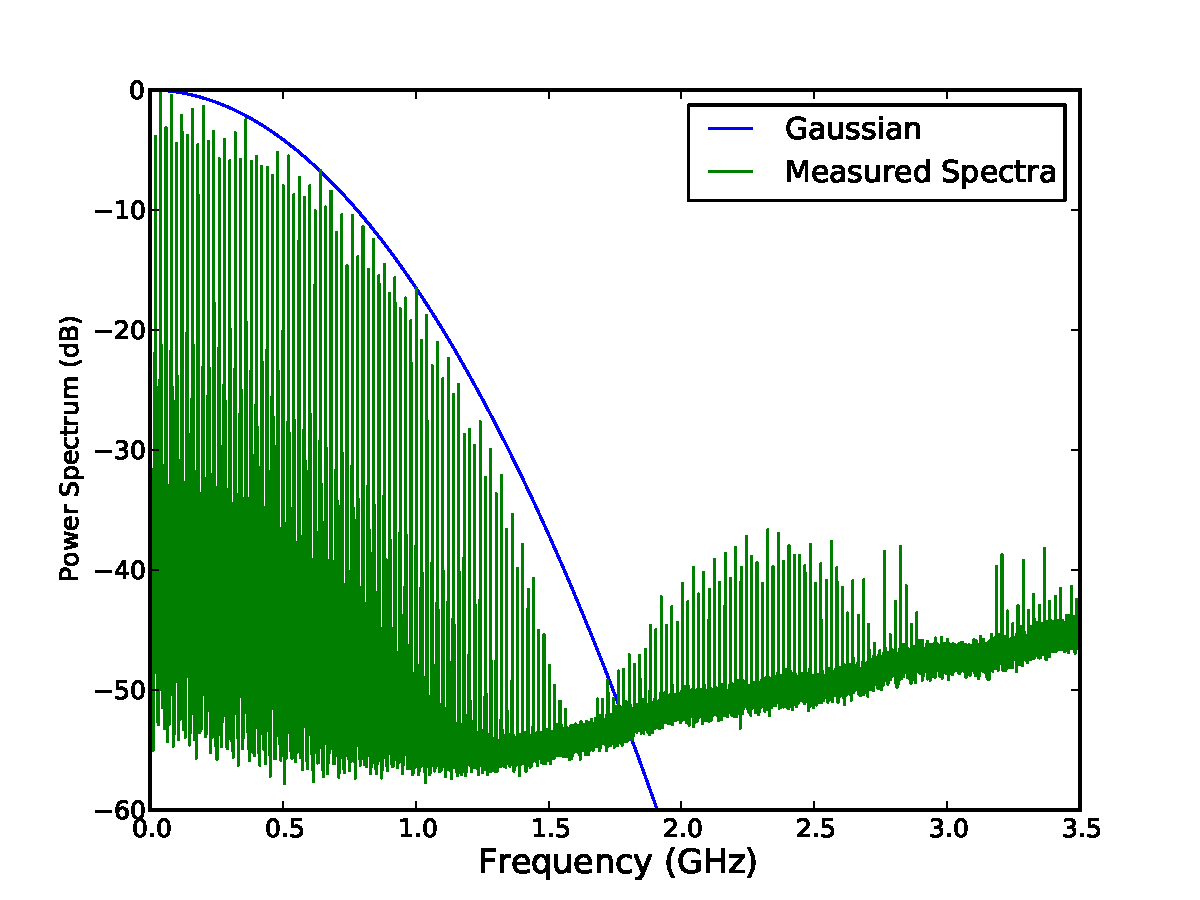
\includegraphics[width=0.45\textwidth]{Wakefields_and_Impedances/figures/beam_spectra_power_gauss_meas_12ns.pdf}
\label{fig:gauss_meas_freq}
}
\subfigure[]{
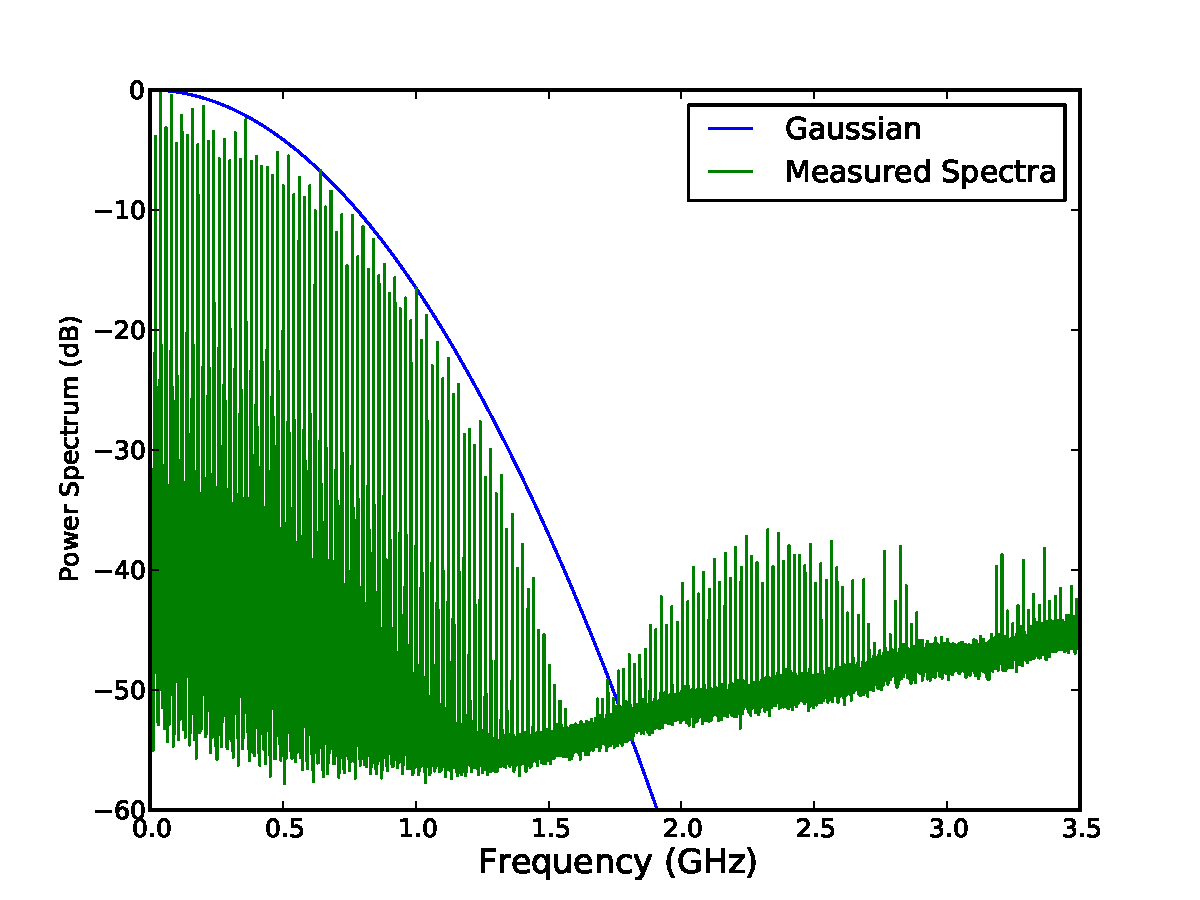
\includegraphics[width=0.45\textwidth]{Wakefields_and_Impedances/figures/beam_spectra_power_gauss_meas_12ns.pdf}
\label{fig:gauss_meas_time}
}
\caption{A comparison of \ref{fig:gauss_meas_freq} a measured beam power spectrum and a Gaussian bunch of the same bunch length in the frequency domain and \ref{fig:gauss_meas_time} the resulting time domain beam profile. The Gaussian has a bunch length (4$\sigma_{z}$ = 1.2ns). Measured spectrum taken by P. Baundrenghien et al \cite{Baudrenghien:LHCPowSpec}.}
\label{fig:measured_gauss}
\end{figure}

As shown by the derivations in Section~\ref{sec:power_loss}, asides from the longitudinal impedance of the device under consideration the longitudinal profile of the circulating bunches also contributes to the power loss in the machine. In past works it has generally been assumed that bunches in accelerators have a Gaussian profile \cite{Grudiev:LongTransSecCol}, given by

\begin{equation}
\lambda \left( t \right) = e^{\frac{-t^{2}}{2\sigma^{2}}}
\label{eqn:gauss}
\end{equation}

where $4\sigma_{z} = t_{b}$ when approaching the analytical treatment of beam induced heating, both single-bunch and multi-bunch. Recent measurements of the power spectrum of particle beams, especially in the LHC \cite{Baudrenghien:LHCPowSpec} have shown characteristics that the Gaussian profile does not predict, for example the high frequency secondary peak as seen in Fig.~\ref{fig:measured_gauss}. To make more realistic predictions of heat loss due to beam impedance in the machine it is thus necessary to find bunch profiles which reproduce this behaviour.

A number of different longitudinal bunch profiles have been investigated in the past. Here we shall look at 3 other bunch profiles; a parabolic line density (see Eqn.~\ref{eqn:para_profile}), cos$^{2}$ (see Eqn.~\ref{eqn:cos_profile}) and a water-bag (see Eqn.~\ref{eqn:water_bag_profile}).

\begin{equation}
\rho\left( t \right) = \int^{\infty}_{-\infty} \lambda \left( \omega \right) e^{j\omega t} d\omega = 
\begin{cases}1-\left( \frac{2t} {t_{b}} \right)^{2} &\textrm{if $| t/2 | \leq t_{b}$}\\
0								&\textrm{if $| t | > t_{b}/2$}
\end{cases}
\label{eqn:para_profile}
\end{equation}

\begin{equation}
\rho\left( t \right) = \int^{\infty}_{-\infty} \lambda \left( \omega \right) e^{j\omega t} d\omega = 
\begin{cases}
cos^{2}\left( \frac{\pi t} {t_{b}} \right) &\textrm{if $| t/2 | \leq t_{b}$}\\
0								&\textrm{if $| t | > t_{b}/2$}
\end{cases}
\label{eqn:cos_profile}
\end{equation}

\begin{equation}
\rho\left( t \right) = \int^{\infty}_{-\infty} \lambda \left( \omega \right) e^{j\omega t} d\omega = 
\begin{cases}
\sqrt{1-\left( \frac{2t}{t_{b}}\right)^{2}} &\textrm{if $| t/2 | \leq t_{b}$}\\
0								&\textrm{if $| t | > t_{b}/2$}
\end{cases}
\label{eqn:water_bag_profile}
\end{equation}

The corresponding frequency domain profiles are given by Eqn.~\ref{eqn:para_profile_freq} for the parabolic profile, Eqn.~\ref{eqn:cos_profile_freq} for the cos$^{2}$ profile, and Eqn.~\ref{eqn:water_bag_profile_freq} for the waterbag profile,

\begin{equation}
 \lambda \left( f \right) = 
\label{eqn:para_profile_freq}
\end{equation}

\begin{equation}
\lambda \left( f \right)  = \frac{sin \left( \pi f t_{b} \right)}{\pi f t_{b} \left[ 1 - \left( f t_{b} \right) \right]}
\label{eqn:cos_profile_freq}
\end{equation}

\begin{equation}
\lambda \left( f \right) = 
\label{eqn:water_bag_profile_freq}
\end{equation}

\begin{figure}
\begin{center}
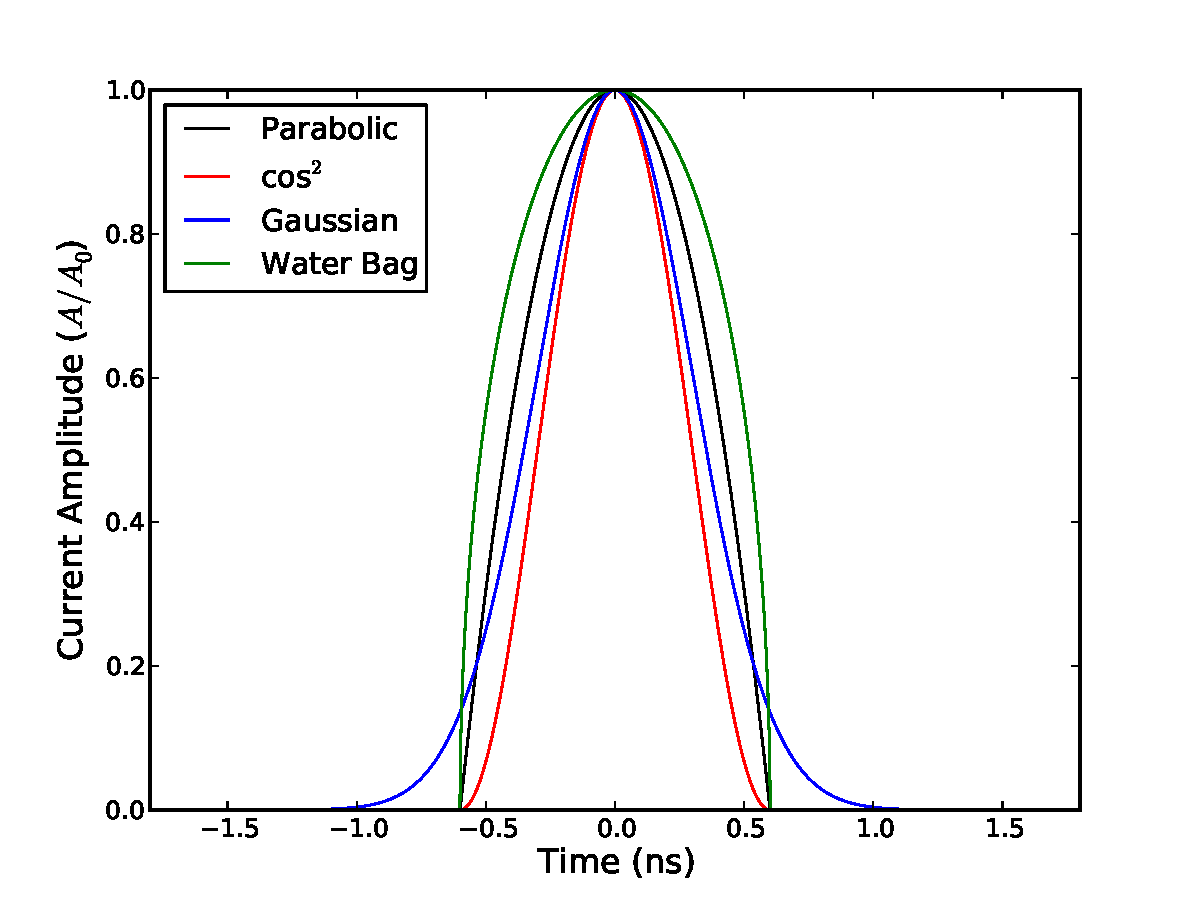
\includegraphics[width=0.65\textwidth]{Wakefields_and_Impedances/figures/bunch_profile_12ns.pdf}
\end{center}
\label{fig:time_bunch_profiles}
\caption{The longitudinal bunch profile of a number of bunch distributions. Note that all of these are normalised to have a peak bunch current of 1. For the Gaussian distribution the bunch length is the 4$\sigma$ value. The bunch length $\tau_{b} = 1.2ns$}
\end{figure}

\begin{figure}
\subfigure[]{
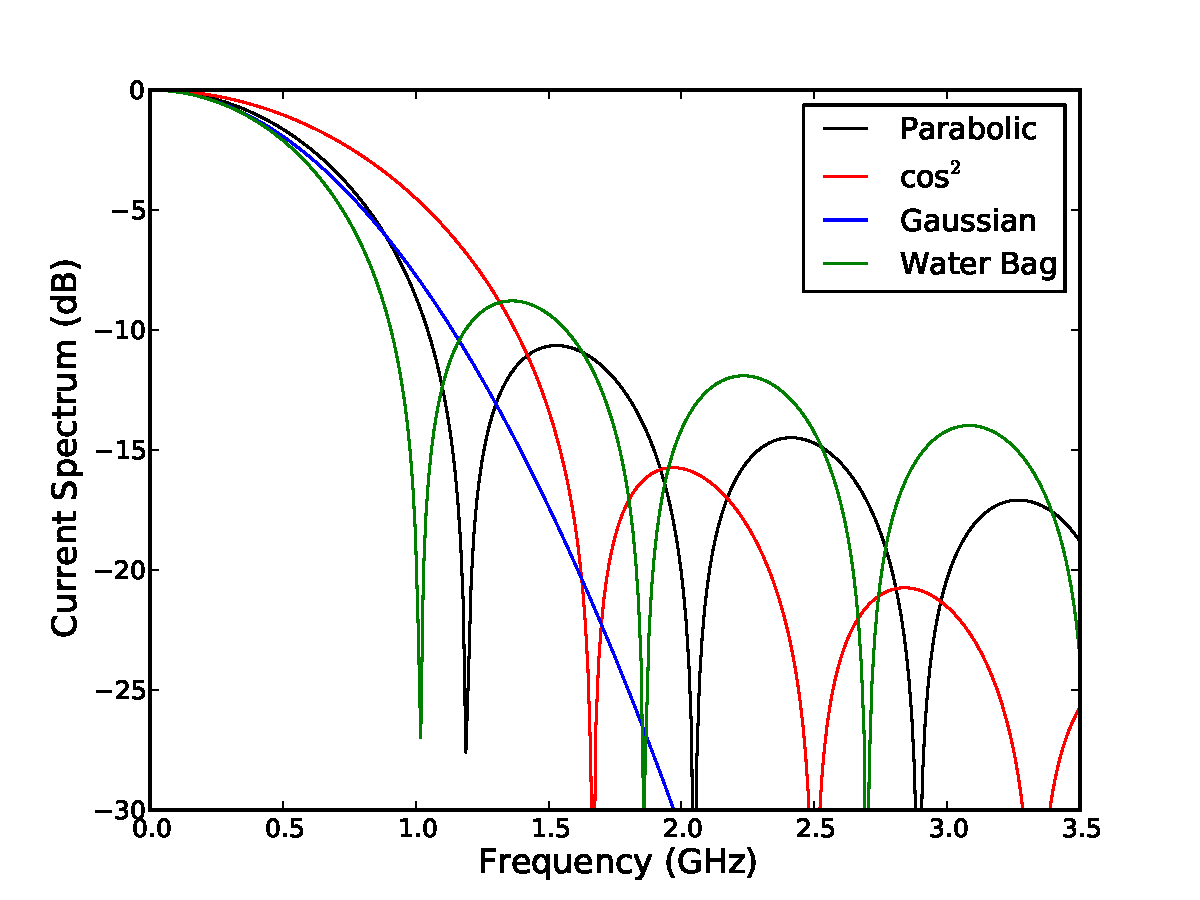
\includegraphics[width=0.45\textwidth]{Wakefields_and_Impedances/figures/current_spectrum_12ns.pdf}
\label{fig:current_spec}
}
\subfigure[]{
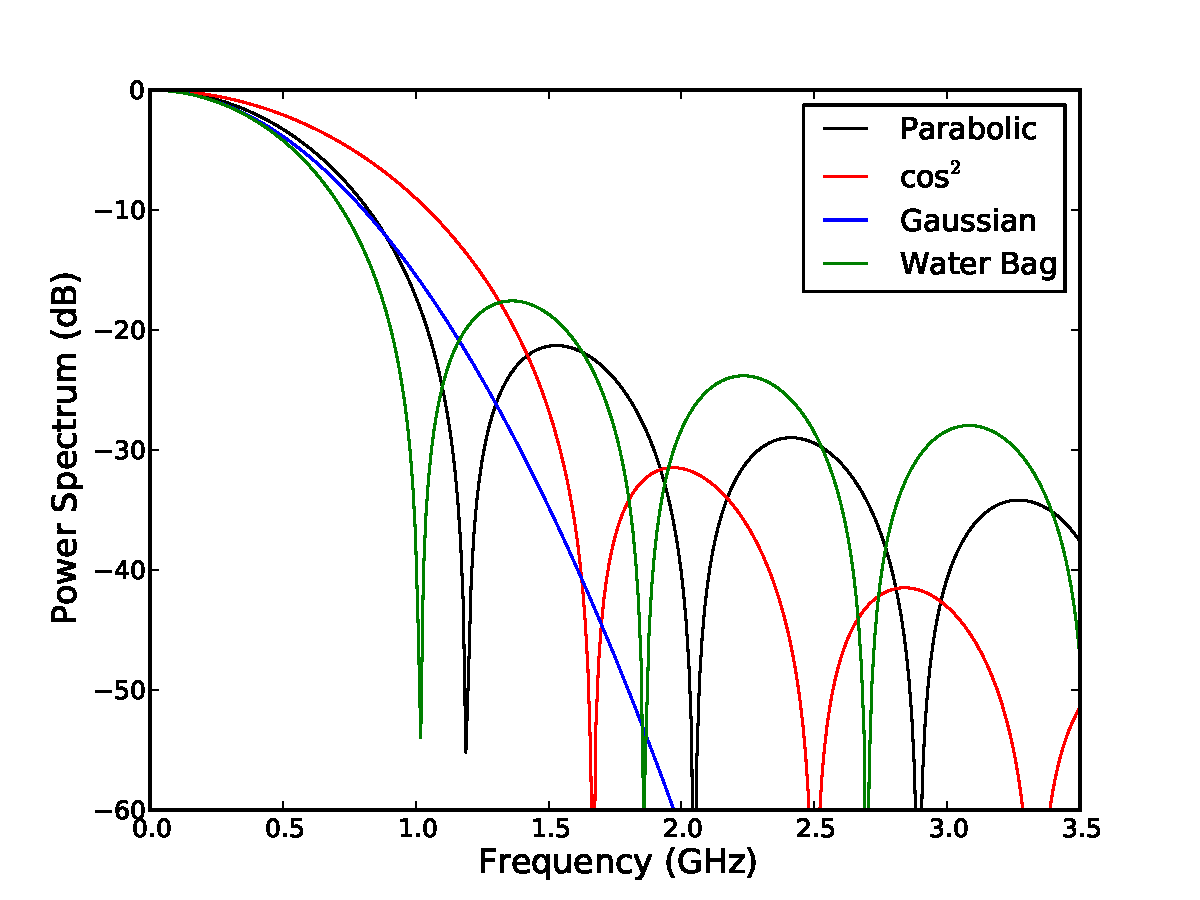
\includegraphics[width=0.45\textwidth]{Wakefields_and_Impedances/figures/power_spectrum_12ns.pdf}
\label{fig:power_spec}
}
\caption{The frequency domain \ref{fig:current_spec} current spectrum and \ref{fig:power_spec} power spectrum for a number of different bunch profiles with a bunch length $\tau_{b} = 1.2ns$.}
\label{fig:freq_dom_prof}
\end{figure}

The comparison of these bunch profiles in the time domain are shown in Fig.~\ref{fig:time_bunch_profiles}. Note all bunch currents are normalised to their peak value. The corresponding current and power spectrums are shown in Fig.~\ref{fig:freq_dom_prof}. There are several things to note about these spectra; firstly that the non-infinite distribution of the non-Gaussian bunch profiles gives rise to a number of high frequency lobes in the power spectrum, and secondly the interval of these nodes depends heavily on the bunch profile.

\begin{figure}
\subfigure[]{
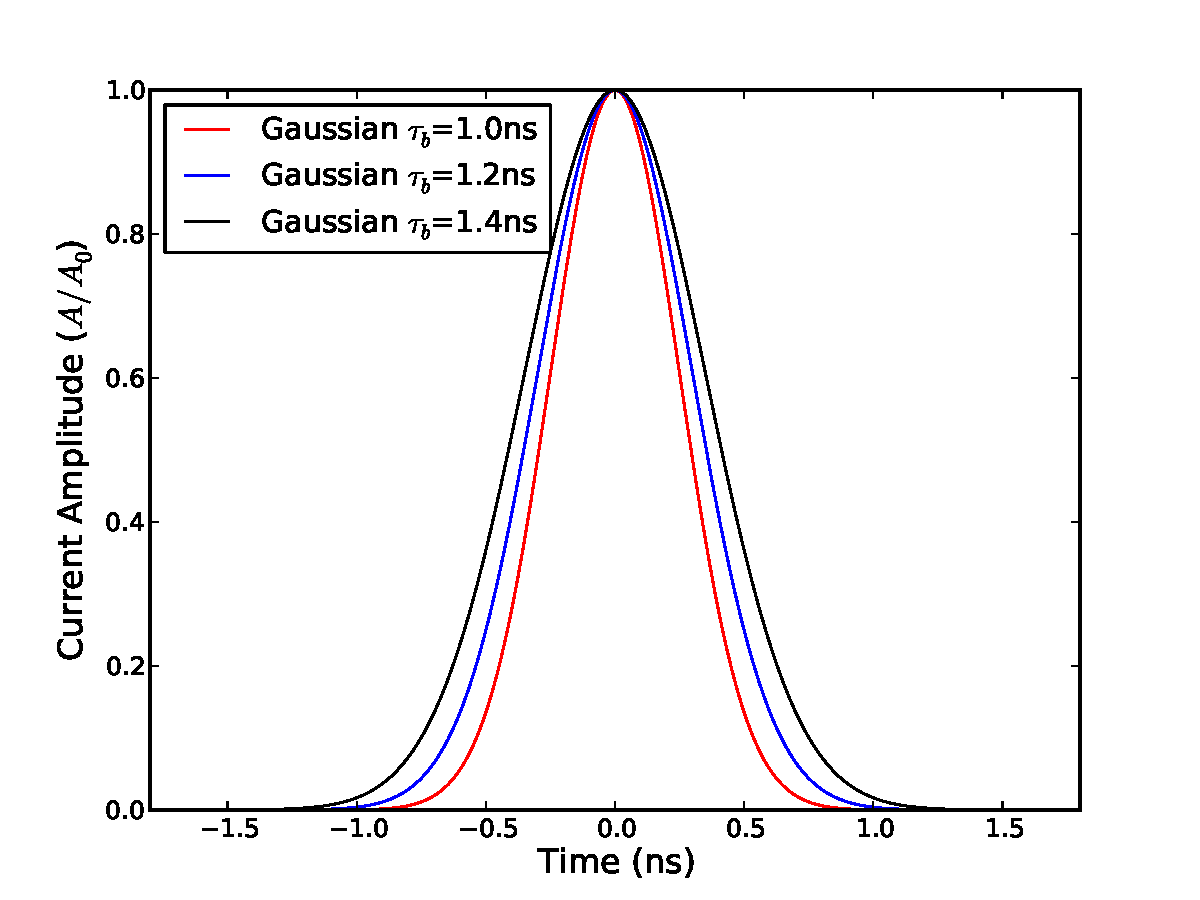
\includegraphics[width=0.45\textwidth]{Wakefields_and_Impedances/figures/gaussian_time_dom_diff_lengths.pdf}
\label{fig:change_len_time_gauss}
}
\subfigure[]{
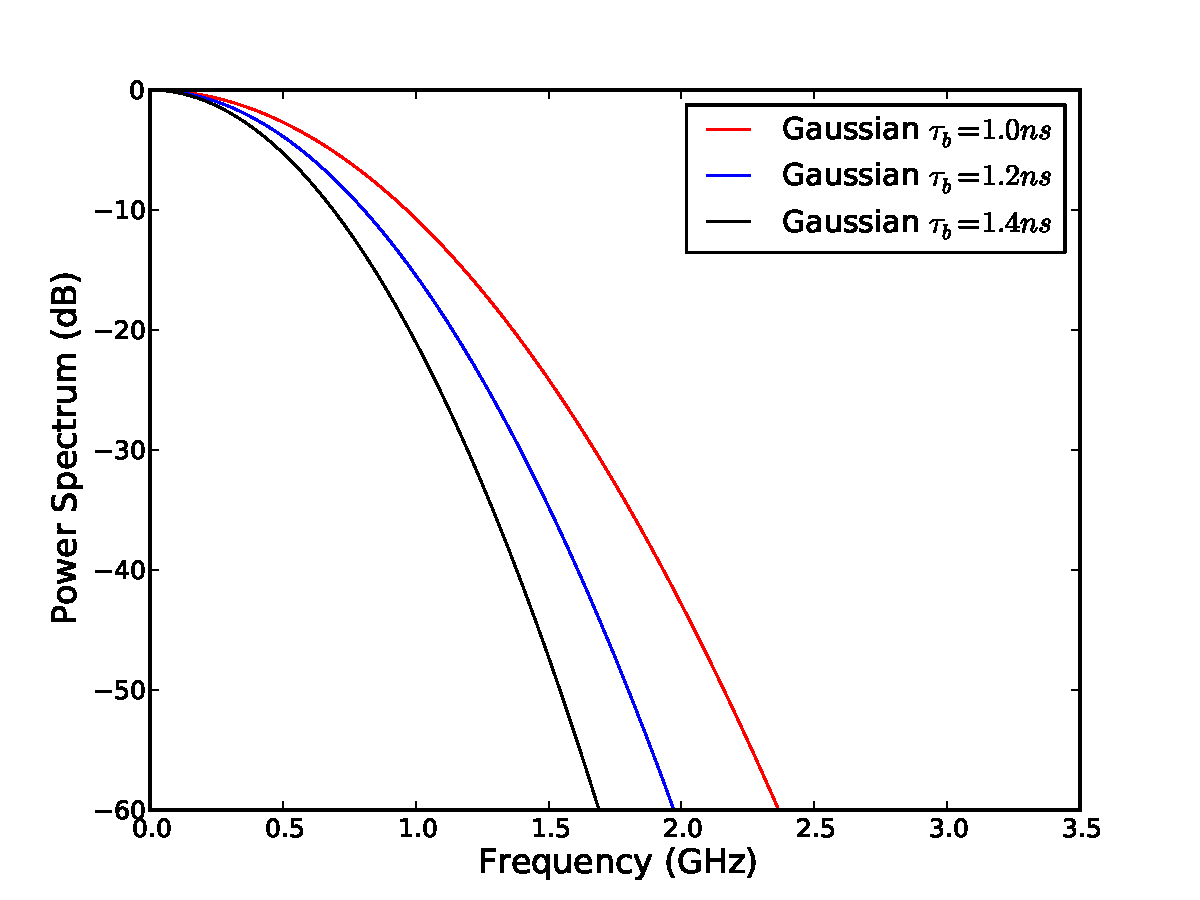
\includegraphics[width=0.45\textwidth]{Wakefields_and_Impedances/figures/gaussian_power_spec_diff_lengths.pdf}
\label{fig:change_len_freq_gauss}
}
\caption{\ref{fig:change_len_time_gauss} The longitudinal profile and the \ref{fig:change_len_freq_gauss} associated bunch power spectrum for a number of bunch lengths assuming a Gaussian bunch profile.}
\label{fig:diff_bunch_len_gauss}
\end{figure}

\begin{figure}
\subfigure[]{
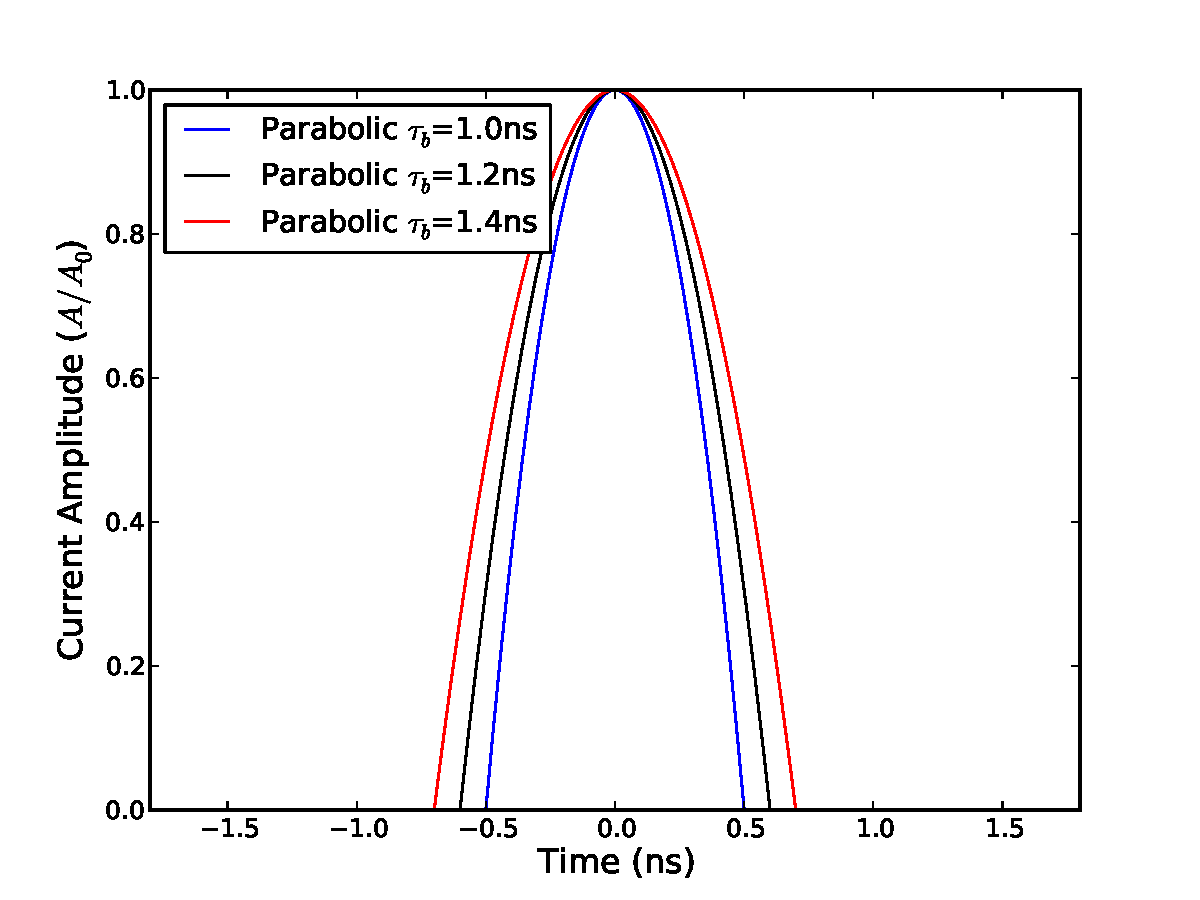
\includegraphics[width=0.45\textwidth]{Wakefields_and_Impedances/figures/current_amp_para_change.pdf}
\label{fig:change_len_time_para}
}
\subfigure[]{
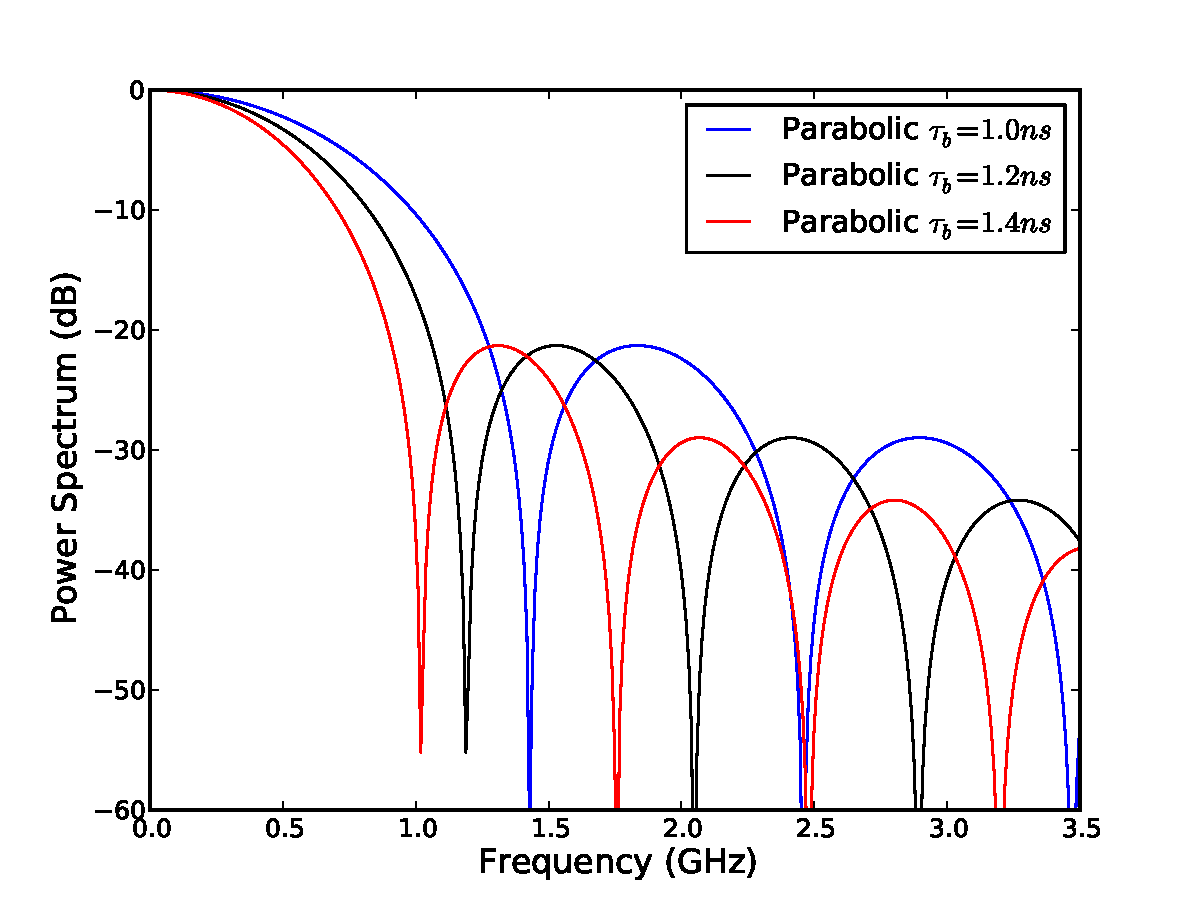
\includegraphics[width=0.45\textwidth]{Wakefields_and_Impedances/figures/freq_power_para_change.pdf}
\label{fig:change_len_freq_para}
}
\caption{\ref{fig:change_len_time_para} The longitudinal profile and the \ref{fig:change_len_freq_para} associated bunch power spectrum for a number of bunch lengths assuming a parabolic bunch profile.}
\label{fig:diff_bunch_len_para}
\end{figure}

To illustrate more clearly the effect of changing the bunch length on the power spectrum, a number of bunch profiles and the corresponding power spectra with different bunch lengths are shown in Fig~\ref{fig:diff_bunch_len_gauss}. Firstly, consider a Gaussian bunch profile. It can be seen in Fig.~\ref{fig:diff_bunch_len_gauss} that by increasing the bunch length that the magnitude at high frequencies is decreased quite substantially. If we consider a finite bunch profile (non-Gaussian), we note that we have high frequency lobes. The peak frequency of these lobes depends on the bunch length, as illustrated using a parabolic bunch profile for bunch lengths $\tau_{b} = 1ns, 1.2ns, 1.4ns$ in Fig.~\ref{fig:diff_bunch_len_para}. As the bunch length is increased the lobes move to lower frequencies, and the width of the first branch decreases. Similar behaviour is observed with the cos$^{2}$ and water-bag bunch profiles.

\begin{figure}
\begin{center}
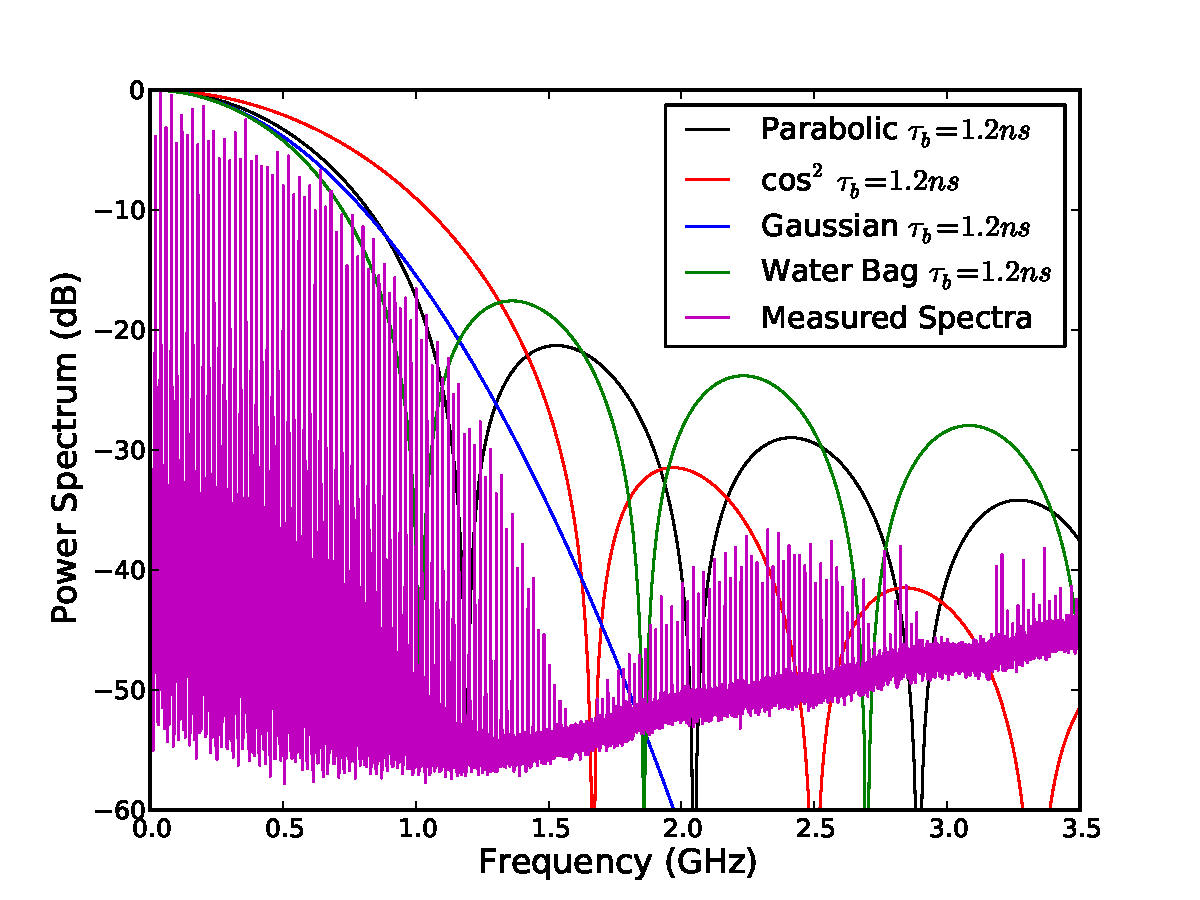
\includegraphics[width=0.65\textwidth]{Wakefields_and_Impedances/figures/beam_spectra_power_12ns.pdf}
\end{center}
\caption{A comparison of a measured beam power spectrum and a number of analytical bunch profiles assuming a bunch length of 1.2ns.}
\label{fig:power_all}
\end{figure}

Finally, a comparison of a measured bunch power spectra and the analytical power spectra is shown in Fig.~\ref{fig:power_all}. It can be seen that whilst it is possible to replicate some of the properties of the measured spectrum, an exact replication is non-trivial. Further investigation into the appropriate bunch profile is ongoing.



% Introduce a number of longitudinal profiles in time domain - gaussian, parabolic line density, cos^2, water bag - comments of realism (gaussian being infinite) - truncated gaussian
% Comparison in the frequency domain - firstly gaussian compared to truncated gaussian - infinite tails reduce the magnitude of the higher frequency components and lobe
% Gaussian, parabolic, cos^2 - all with the same bunch length
% Using the above examples try using a number of different bunch lengths to illustrate how they change (gaussian - just extends further, parabolic, cos^2 lobe frequency changes)
% Finally - comparison to measured spectra to illustrate changes in bunch length and frequency components as bunch is ramped and squeezed

\subsubsection{Beam induced heating due to a low Q impedance}

For an impedance with a characteristic Q that is small (Q $<$ 10), it can be seen that the impedance peak will interact substantially with a number of beam harmonics (see Fig.~\ref{fig:low_q_harmonics}) due to the broad frequency range it occupies.

\begin{figure}
\begin{center}
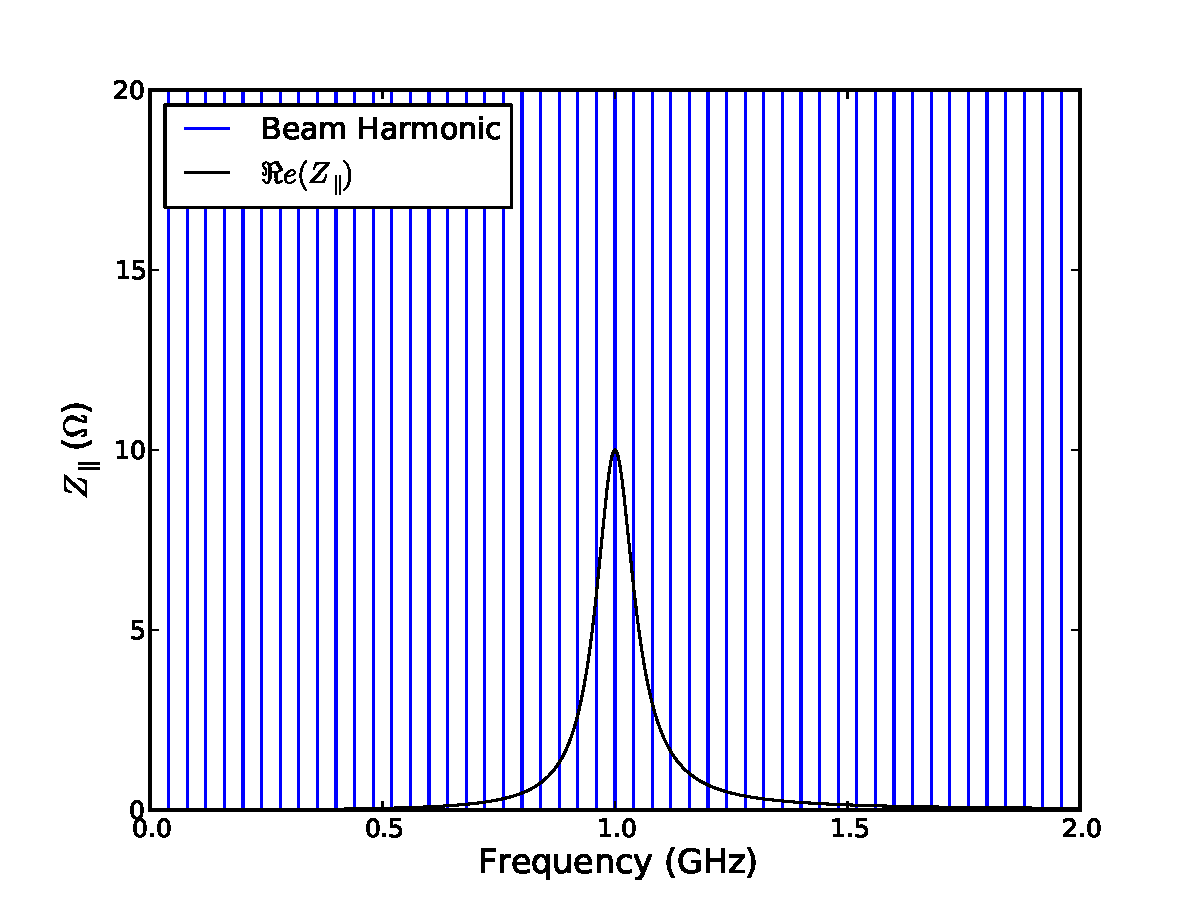
\includegraphics[width=0.65\textwidth]{Wakefields_and_Impedances/figures/low_q_10_resonance_beam_harmonics.pdf}
\end{center}
\caption{The beam harmonics of a beam with a bunch spacing of 25ns overlayed on the real component of the longitudinal impedance an example of a low Q impedance ($R_{s}=10\omega$, Q = 10, $f_{res}=1GHz$). The blue lines represent the frequency of a beam harmonic, not necessarily the magnitude of the power spectrum at that point. Note that a number of beam harmonics overlay non-zero impedance values.}
\label{fig:low_q_harmonics}
\end{figure}

Further investigation of the longitudinal beam spectrum reveals that there is significant structure between the major harmonics (which are due to the bunch spacing of the beam) which can be attributed to the other time structures of the beam, for example the bunch train spacing, or the interval between the pilot bunch train and the subsequent bunch train. As such the treatment of the estimation of beam losses requires a broad spectrum approach. If we consider Eqn.~\ref{eqn:heating-gen} we see that we can treat the power losses in an integral form. We can observe a number of properties using this assumption. The power loss is proportional to the beam properties in the following manner:

\begin{enumerate}
\item{$P_{loss} \propto N^{2}$}
\item{$P_{loss} \propto n_{bunch}$}
\end{enumerate}

\subsubsection{Beam induced heating due to a high Q impedance}

In contrast to the overlap of the beam spectrum with a low Q impedance, for a high Q impedance only one beam harmonic lies upon the resulting impedance to any significant quantity. This is illustrated in Fig~\ref{fig:high_q_harmonics}. If we consider Eqn \ref{eqn:heating-gen} and consider the situation where

\begin{equation}
\left( 2 \left| \lambda \left(p \omega_{rev}n_{bunch} \right)  \right|^{2}  \Re{}e \left( Z_{\parallel} \left(p \omega_{rev}n_{bunch}\right) \right) \right) = 
\begin{cases}
\left( 2 \left| \lambda \left( \omega_{res} \right)  \right|^{2}  \Re{}e \left( Z_{\parallel} \left( \omega_{res} \right) \right) \right) &\textrm{if $p \omega_{rev} n_{bunch} = \omega_{res}$}\\
0								&\textrm{if $p \omega_{rev} n_{bunch} != \omega_{res}$}
\end{cases}
\label{eqn:single_harmonic_profile}.
\end{equation}

\begin{figure}
\begin{center}
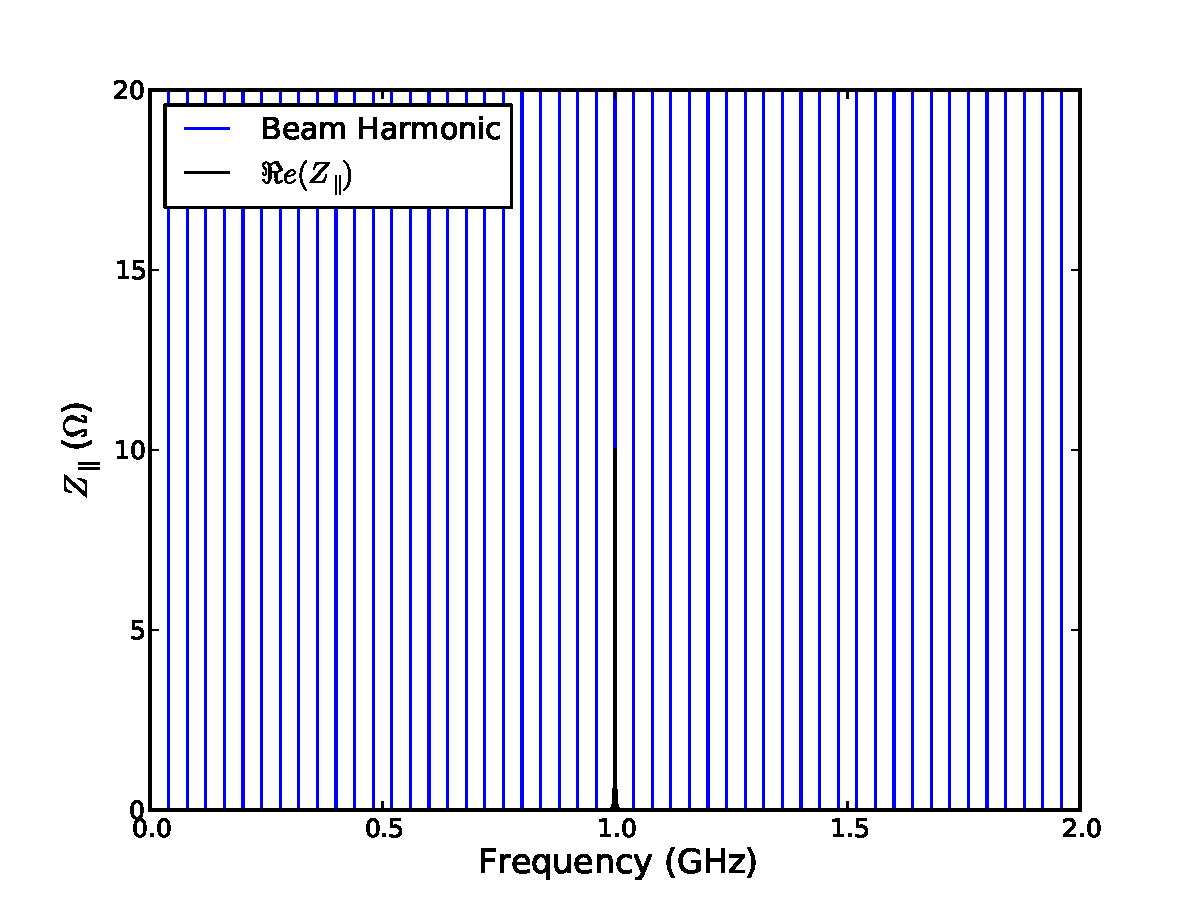
\includegraphics[width=0.65\textwidth]{Wakefields_and_Impedances/figures/high_q_1000_resonance_beam_harmonics.pdf}
\end{center}
\caption{The beam harmonics of a beam with a bunch spacing of 25ns overlayed on the real component of the longitudinal impedance of a sample of a high Q impedance ($R_{s}=10\Omega$, Q = 1000, $f_{res}=1GHz$). The blue lines represent the frequency of a beam harmonic, not necessarily the magnitude of the power spectrum at that point. Note that only a single beam harmonic overlays a non-zero impedance values.}
\label{fig:high_q_harmonics}
\end{figure}

It can then be seen that Eqn~\ref{eqn:heating-gen} simplifies to

\begin{equation}
P_{loss} = \left( \omega_{rev}eN_{b}n_{bunch}  \right)^{2}  \left( 2 \left| \lambda \left( \omega_{res} \right)  \right|^{2}  \Re{}e \left( Z_{\parallel} \left(\omega_{res} \right) \right) \right). 
\label{eqn:heating-high-q}
\end{equation}

The following properties can subsequently be seen as a result:

\begin{enumerate}
\item{$P_{loss} \propto N^{2}$}
\item{$P_{loss} \propto n_{bunch}^{2}$, provided that the resonant frequency of the resonance continues to coincide with a beam harmonic.}
\end{enumerate}

\subsubsection{Some Examples of the Beam-Induced Heating}

In this section we shall illustrate some important factors that have been covered in previous sections. In particular, the interaction of different bunch profiles at different bunch lengths with an example cavity resonance will be covered in some detail to illustrate how the estimated heating can change drastically depending on higher frequency lobes in the beam current spectrum. In addition, the heating due to two particle beams in the same vacuum chamber shall be briefly covered for interest.

\subsubsection{The Effect of Bunch Length on Power Loss}

As can be seen in Figs.~\ref{fig:freq_dom_prof} and Fig~\ref{fig:diff_bunch_len_para}, the bunch profile and the bunch length can significantly alter the magnitude of the beam current at higher frequencies. To illustrate this, let us consider two resonant impedances, one broadband $Z_{bb}$ and one narrow band $Z_{nb}$ impedance, characterised by having a low-$Q$ and a high-$Q$ respectively. Both impedances shall have the same resonant shunt impedance $R_{s} = 100\Omega$. The broadband impedance shall have a $Q_{bb}=1$, and the narrow band impedance $Q_{nb}=1000$. The resonant frequency will be changed to illustrate effects in different regimes of the bunch length and of different bunch profiles.

We shall use the Gaussian bunch profile and the $cos^{2}$ bunch profile for these examples. The Gaussian is useful to illustrate the effect of just changing the bunch length, and the $cos^{2}$ due to the presence of a high frequency lobe in it's frequency domain current spectrum. The $cos^{2}$ frequency domain current profile is given by

\begin{equation}
I \left( \omega \right) = \frac{sin \left( \omega \tau_{b}/2 \right)}{ \omega \tau_{b}/2 \left[ 1 - \left(  \omega \tau_{b}/2 \right)^{2}  \right]}.
\end{equation}

\begin{figure}
\begin{center}
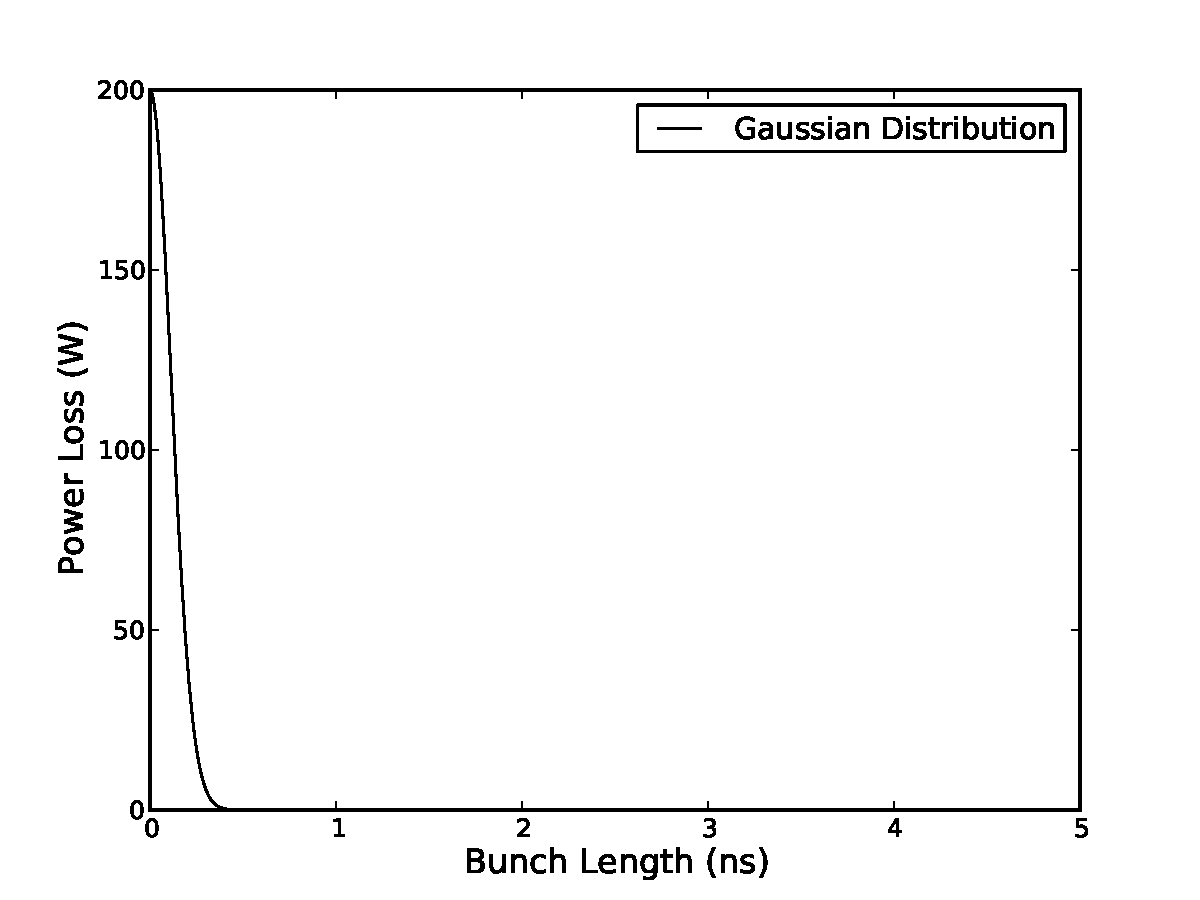
\includegraphics[width=0.8\textwidth]{Wakefields_and_Impedances/figures/heating_narrowband_gauss_bunch_length.pdf}
\end{center}
\caption{The change in power loss due to a narrow band resonance characterised by $\omega_{0} = 2GHz$, $R_{s} = 100\Omega$, $Q = 1000$ with a Gaussian bunch distrbution of different lengths.}
\label{fig:bunch_length_heat_narrow}
\end{figure}

First we shall consider a narrow band impedance which has a resonant frequency $\omega_{0} =2GHz$ which falls upon a beam harmonic such that $\omega_{0}=n\omega_{rev}$, where $n$ is an integer. It should be noted that for other cases the contribution of these sources of heating is negligible due to the small beam current at this frequency. There are two extreme cases; that of  $\omega_{0} \gg 1/\tau_{b}$, in which it can be seen that the current spectrum will be negligible at the frequency of the impedance, and $\omega_{0} \ll 1/\tau_{b}$ where the beam current spectrum is essentially the same as the DC spectral component. The transition in this intervening regime is shown in Fig~\ref{fig:bunch_length_heat_narrow}, assuming a bunch current of 1A. It can be seen that in this case the heating falls drastically as the bunch length increases.

If we instead consider a cos$^{2}$ distribution we instead see the effect of the secondary lobes in the beam current spectrum. The power loss with bunch length is shown in Fig.~\ref{fig:bunch_length_heat_narrow} in comparison to that of the Gaussian profile. The beam power spectrum for a number of different bunch lengths are shown with the real component of the longitudinal impedance in Fig.~\ref{fig:imp_profile_cos}. Here it can be clearly seen that the intersection of the secondary lobe with the resonant impedance causes a peak in the power lost by the beam, highlighting the neccessity to be aware of the frequencies of resonant impedances with relation to the beam harmonics.


\begin{figure}
\subfigure[]{
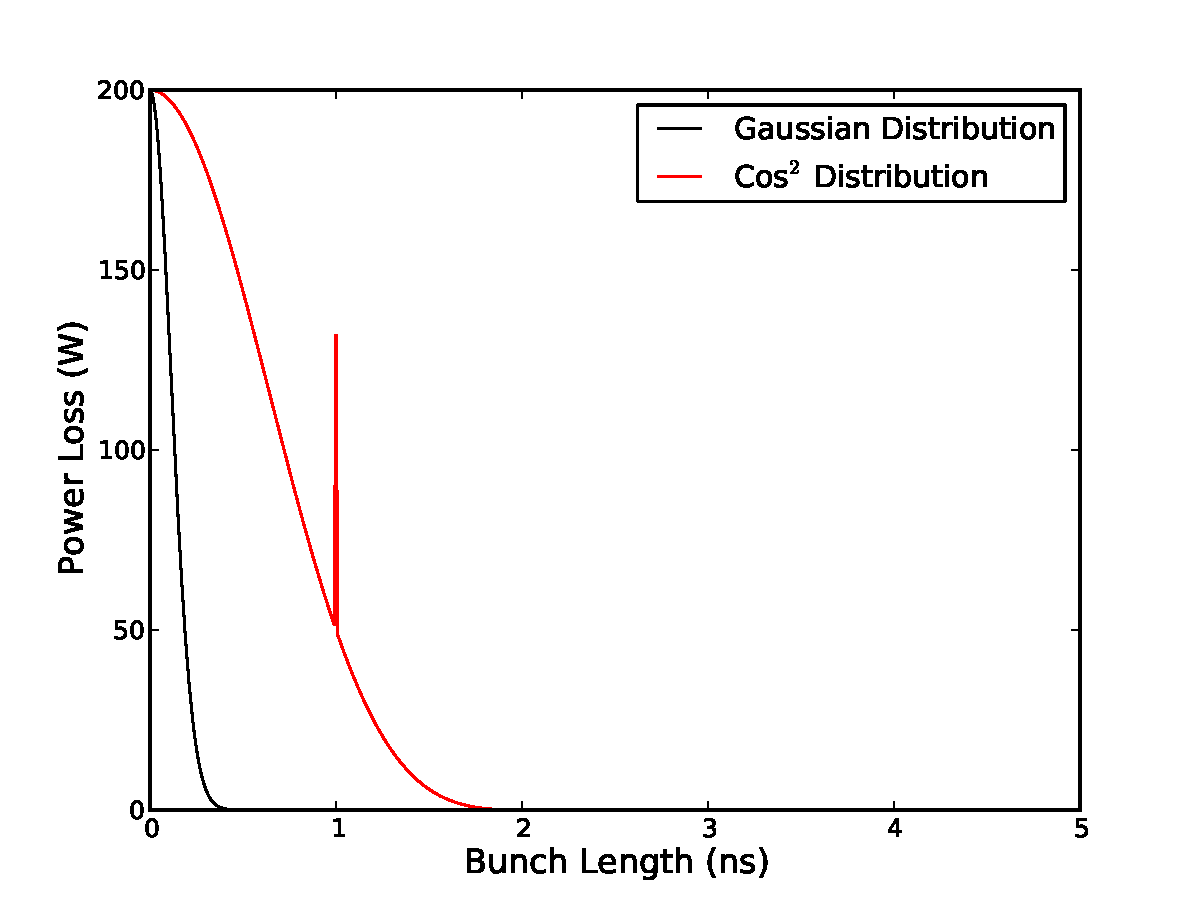
\includegraphics[width=0.5\textwidth]{Wakefields_and_Impedances/figures/heating_narrowband_gausscos_bunch_length.pdf}
\label{fig:long_imp_narrow_current}
}
\subfigure[]{
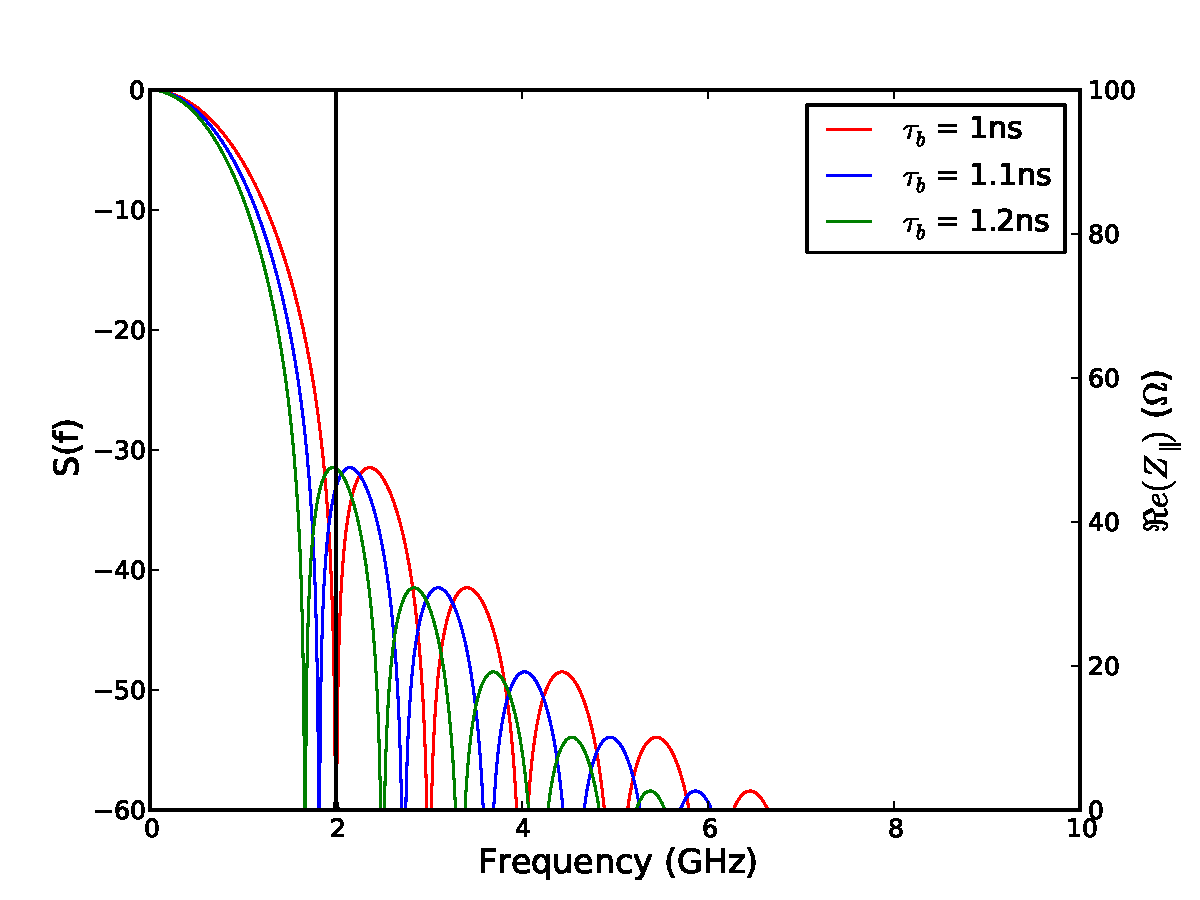
\includegraphics[width=0.5\textwidth]{Wakefields_and_Impedances/figures/impedance_and_power_cos_res.pdf}
\label{fig:imp_profile_cos}
}
\caption{\ref{fig:long_imp_narrow_current} The change in power loss due to a narrow band resonance characterised by $\omega_{0} = 2GHz$, $R_{s} = 100\Omega$, $Q = 1000$ interacting with a cos$^{2}$ bunch distribution with different bunch lengths. The impedance and the beam power spectrum are shown in \ref{fig:imp_profile_cos} to illustrate how this relates to the power loss.}
\end{figure}

\begin{figure}
\subfigure[]{
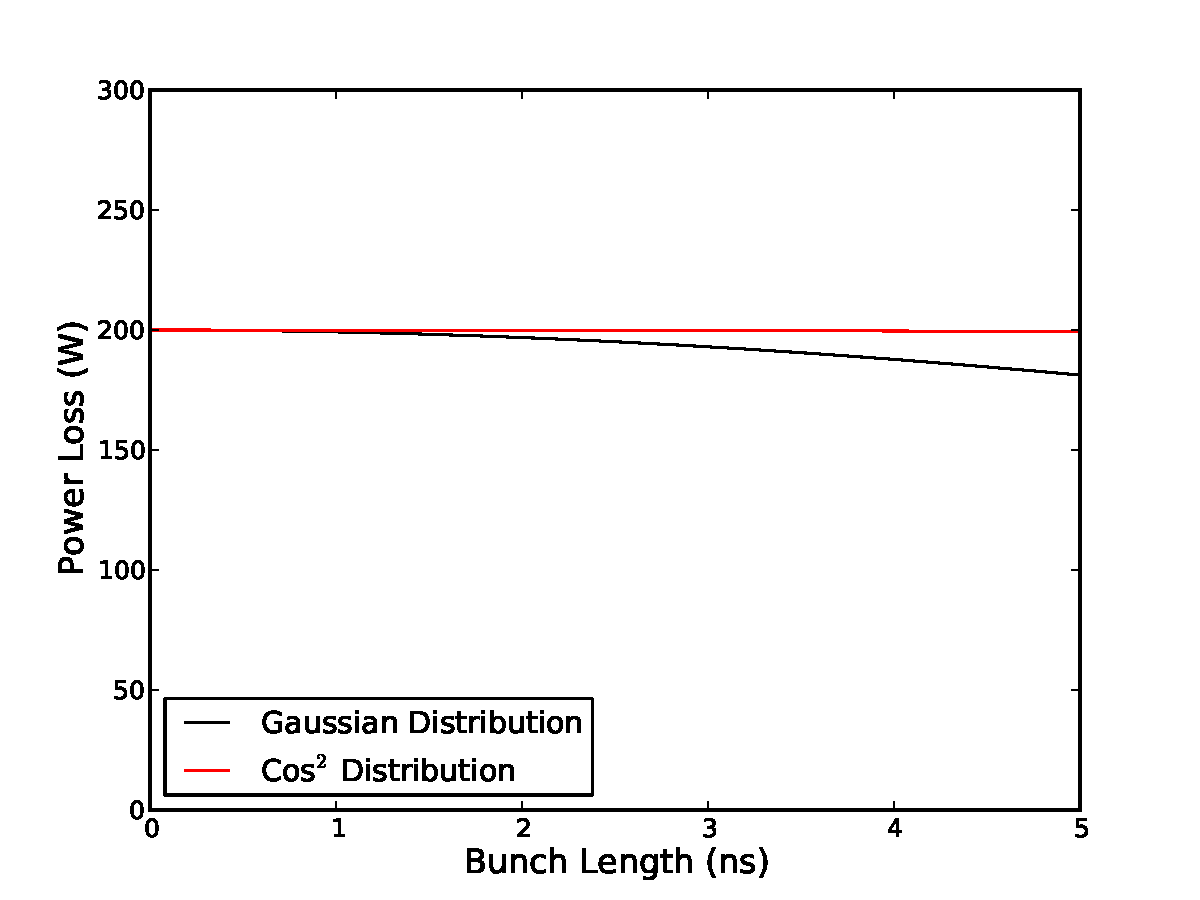
\includegraphics[width=0.5\textwidth]{Wakefields_and_Impedances/figures/heating_broadband_gausscos_bunch_length.pdf}
\label{fig:broadband_heat_bunch_len}
}
\subfigure[]{
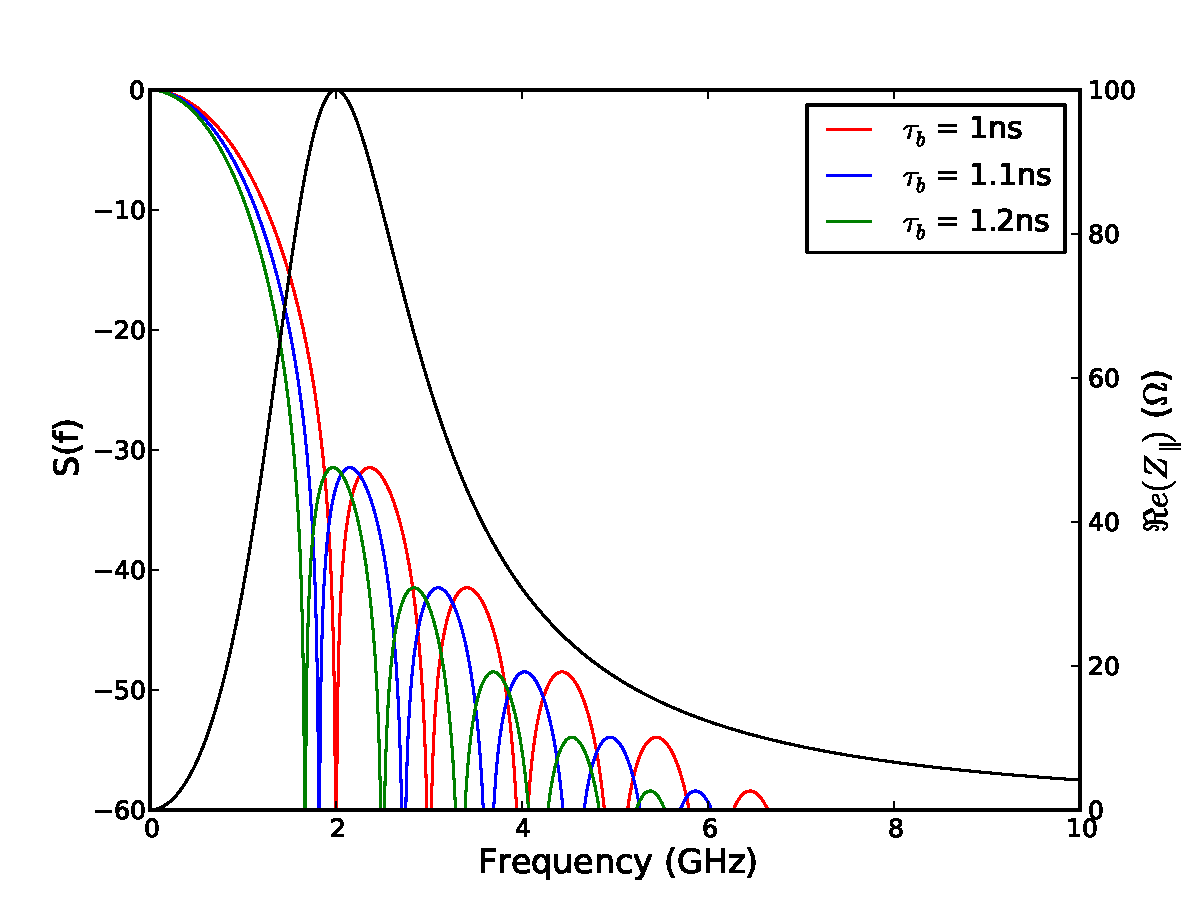
\includegraphics[width=0.5\textwidth]{Wakefields_and_Impedances/figures/impedance_and_power_cos_res_broad.pdf}
\label{fig:broadband_power_loss}
}
\caption{\ref{fig:broadband_heat_bunch_len} The change in power loss due to a narrow band resonance characterised by $\omega_{0} = 2GHz$, $R_{s} = 100\Omega$, $Q = 1$ interacting with a cos$^{2}$ bunch distribution with different bunch lengths. The impedance and the beam power spectrum are shown in \ref{fig:broadband_power_loss} to illustrate how this relates to the power loss.}
\end{figure}


For the broadband heating we shall consider a resonant impedance defined by the following parameters, $\omega_{0} = 2GHz$, $Q=1$, $R_{s}=100\Omega$. To account for the multiple beam harmonics that will interact with the resonance, it is assumed that the beam harmonics in this case occur at $20$MHz intervals. The impedance and the beam power spectrum is shown in Fig.~\ref{fig:broadband_heat_bunch_len} and the resulting power loss in Fig.~\ref{fig:broadband_power_loss} where it can be seen that the power loss decreases slowly with increasing bunch length. This is due to the significant contribution to the power loss at low frequencies, in which the component of the beam power spectrum decreases only marginally due to the decreasing bunch length.

\subsubsection{Beam-Induced Heating due to two traversing beams}

Previous work \cite{Grudiev:twoBeamCol} has investigated the effect of two beams in a vacuum on the beam-induced heating. This is restated here for the sake of completeness.

To begin, consider the two currents $I_{b1} = I_{0}e^{i\phi_{1}}$ and $I_{b1} = -I_{0}e^{i\phi_{2}}$ representing two counter rotating beams. $I_{0}$ represents the beam current, and $\phi_{1/2}$ the phase of beam 1 and beam 2 respectively. Each beam also sees a seperate potential when it traverses the impedance, given by $V_{b1} = \int_{b1} E_{z} e^{i\omega_{0}z/c} dz$ and $V_{b2} = \int_{b2} E_{z} e^{i\omega_{0}z/c} dz$ respectively. By Ohms law it can then be seen that

\begin{equation}
\begin{pmatrix}
V_{b1} \\
V_{b2}
\end{pmatrix}
=
\begin{bmatrix}
Z_{11} & Z_{12} \\
Z_{21} & Z_{22}
\end{bmatrix}
\begin{pmatrix}
I_{b1} \\
I_{b2}
\end{pmatrix}.
\end{equation}

The power loss due to both beams can then be seen to be

\begin{equation}
P_{loss} = \begin{pmatrix}
V_{b1} & V_{b2}
\end{pmatrix}
\begin{pmatrix}
I_{b1} \\
I_{b2}
\end{pmatrix}^{*}.
\end{equation}

In the worst case scenario, the values of the impedance matrix are real, and are equal in value to the peak values of the resonant impedance
\begin{equation}
Z_{11} = 2R^{b1}_{s};\text{    } Z_{22} = 2R^{b2}_{s};\text{    }  Z_{12} = Z_{21} = 2 \sqrt{R^{b1}_{s}R^{b2}_{s}}.
\end{equation}

The power loss then becomes

\begin{equation}
P_{loss} = I_{0}^{2} 2 \left( R_{s}^{b1} +  R_{s}^{b1} - 2\sqrt{R^{b1}_{s}R^{b2}_{s}} cos \left( \delta \phi \right) \right)
\end{equation}

where $\delta \phi = \phi_{1} - \phi_{2}$ is the phase difference between beam 1 and beam 2. This can be found relatively easily by comparing the distance $\delta s$ from a collision IP (location of experiments in the LHC) of the machine. Assuming the beams are ultrarelativistic $\delta \phi = \omega_{rev} 2  \delta s /c$. It can then be seen that the the last term may either reduce or increase the power loss depending on whether $cos\left( \delta \phi \right) = 1$ or $cos\left( \delta \phi \right) = -1$ respectively.


\subsection{Beam Instabilities}

Beam Instabilities is the collective term for a various group of mechanisms which attribute to the degradation of beam properties during the circulation of a beam within a synchrotron. These can typically be into a number of different subgroups, summarised below:

\begin{enumerate}
\item{Coherent Effects - Occuring due to the bulk oscillation of the bunch(es)}
\item{Incoherent Effects - Occuring due to a mechanism that effects particles dependent on their position within in the bunch}
\item{Single-Bunch - Occuring only on the scale of a single bunch}
\item{Multi-Bunch - Occuring due to coupling of the motion between multiple bunches}.
\end{enumerate}

The mechanisms driving these instabilities are multitudinous and of which beam coupling impedance is just one. Others include space charge effects (both direct and indirect)[cite], beam-beam interactions [cite], electron cloud [cite], IBS [cite] amongst others. Here we shall give a brief overview of how these effects cause a degradation in beam operation.

\subsubsection{Tune Shift and Tune Spread} 

As seen in Sec. [ref introduction transverse motion], the transverse equation of motion can be viewed as an oscillatory system. If the particles experience an additional force $ F^{pert}_{x}$ due an external mechanism, not due to the machine optics, it's equation of motion (in the horizontal plane, for example) can be written as

\begin{equation}
\frac{d^{2}x}{ds^{2}} + \left(\frac{Q_{0,x}}{R}\right)^{2} x = \frac{F^{pert}_{x}}{\beta^{2} E_{total}}.
\end{equation}

This subsequently leads to a perturbed oscillation frequency, characterised by the equation

\begin{equation}
\frac{d^{2}x}{ds^{2}} + \left(\frac{Q_{0,x}+ \Delta Q_{pert,x}}{R}\right)^{2} x = 0.
\end{equation}

where $\Delta Q_{pert,x}$ is the part of the betatron frequency caused by the perturbing force. The perturbed tune may also be subsequently be further divided into coherent (the motion of the bunch centroid) and incoherent (motion of individual particles), such that $\Delta Q_{pert,x} = \Delta Q^{coh}_{pert, x} + \Delta Q^{incoh}_{pert, x}$. This seperation leads to the creation of a tune spread in a machine, in which the tune of the beam covers an area of the tune diagram as shown in Fig.~\ref{fig:tune_diag_tune_shift}. In this case particles may be lost when this tune shift causes them to lie upon a major resonance of the beam optics, there by causing cpherent oscillation growth and ultimately particle loss. This leads to negative effects such as emittance growth and lower beam lifetimes.

\begin{figure}
\caption{A tune diagram illustrating the unperturbed tune of a machine, and the resulting perturbed tune and the tune spread as a result of an impedance source. Note that the tune spread has caused some particle to lie upon a major resonance harmonic.}
\label{fig:tune_diag_tune_shift}
\end{figure}

\subsubsection{Longitudinal Single Bunch Instabilities}

Similar to the change in the equations of motion for transverse particles, considering the induced fields in the longitudinal plane produces a perturbation in the longitudinal motion also. This can be thought of as an additional force alongside the electromagnetic force applied by the accelerating cavities. This leads to two interesting phenomenon; potential well distortion, occuring at bunch intensities below some stability criteria, and longitudinal mode coupling instability, or LMCI, above some stability criteria.

The potential well distortion is a direct effect of the incoherent synchrotron tune shift (again, similar in nature to the tune shifts experienced in the transverse plane), which is responsible for a growth in the stable emittance of the bunch. This reveals itself from measurements by a change in the bunch length with increasing bunch intensity, as shown in Fig.~\ref{fig:pot_well_dist}. It should be noted that depending on the source of impedance, the bunch length may increase or decrease depending on whether the bunch is above or below the transition energy of the accelerator.

\begin{figure}
\caption{The change in the bunch length of a proton beam in an SPS like machine due to the effects of a broadband resonator impedance (). Note that the bunch length increases when the beam is above transition, and decreases below transition, as the bunch intensity is increase}
\label{fig:pot_well_dist}
\end{figure}

LMCI occurs when a certain intensity threshold is crossed in the accelerator, leading to a regime known as \emph{turbulent bunch lengthening}. In this mechanism the eigenfrequencies of the natural modes of oscillation of the particles within the RF bucket are shifted due to the changing potential due to the induced wakefield. In high intensity bunches two neighbouring modes may have their frequencies shifted to such an extent that the modes merge into one, thus leading to a case where the modes no longer have only a damped solution, but also a exponentially growing solution. This subsequently leads to the bunch oscillations becoming unstable.

\subsubsection{Transverse Single Bunch Instabilities}

In the transverse plane a number of instability mechanisms apply, which maybe seperated into two forms, those that occur on a time scale much shorter than the synchrotron period, and those that occur on a longer time scale than the synchrotron period. In both cases the leading particles of the bunch, often called the head of the bunch, drives and oscillation in the end, or tails of the bunch. This gives these instabilities their names, the fast head-tail instability, or transverse mode coupling instability (TMCI) and the head-tail instability.

In the case of the fast head-tail instability, the are a number of transverse oscillation modes (see Fig.~\ref{fig:trans_oscillations} for examples), which as with the LMCI experience some frequency shift due to the presence of a wakefield. If the shift is large enough, two of these modes may again couple together, causing an exponential growth of the transverse size of the bunch to occur.

\begin{figure}

\caption{Examples of a number of modes of transverse oscillation. Note that radial and azimuthal modes may occur, as may coupled modes in which the motion of the horizontal and vertical planes is coupled.}
\label{fig:trans_oscillations}
\end{figure}


In the case of the head-tail instability, the movement of a particle from the head of the bunch to the tail and vice versa become important in determining the rate of growth of any unstable modes, and whether any stabilisation mechanisms have sufficient time to damp the growth. This means that the chromaticity of the beam now takes on a great importance, as this relates the betatron tune to the longitudinal motion. This leaves the option of changing the chromaticity of the beam to act as an additional stability mechanism.

\subsubsection{Coupled Bunch Instabilities}

In addition to single bunch instabilities, it is possible in machines where multiple bunches circulate, and possessing wakefields that do not damp in the spacing between bunches (typically caused by high Q resonant impedances), that the motion of the bunch centroids themselves may become coupled together, thus driving what are called coupled bunch instabilities (TCBI for the transverse plane, LCBI for the longitudinal plane). 

This can be understood by imagining the bunch train as a possessing M bunches. This train will then have M possible modes of oscillation with a characteristic frequency of $\omega_{M}$, which may be driven by an impedance at some frequency $\omega_{0}$. If $\omega_{0} \approx n\omega_{M}$ where n is an integer, then the wakefield due to the impedance may drive the oscillation either in a damped fashion (wakefield is out of phase with the oscillation of the mode) or an anti-damped fashion (wakefield is in phase with the oscillation of the mode). In the latter case, this driven oscillation may cause particle losses unless the oscillation is damped via an external mechanism, such as Landau damping or the use of a damper. This motion can occur in both the longitudinal and transverse planes of motion.



\chapter{Beam Based Measurements of Beam Coupling Impedance}
\label{chap:BBmeas}

Beam based measurements are an incredibly useful measurement technique for beam coupling impedance studies. The direct measurements of impedance (either device specific or of the entire machine) provides a reliable comparison to bench top measurements, simulations and analytical calculations. 

There are a number of measurement methods for both the longitudinal and transverse planes using the RF systems and beam instrumentation commonly placed in accelerators. A short introduction to some of the most commonly used of these methods is given here.

\section{Longitudinal Beam Impedance Measurements}

To understand the longitudinal impedance measurements a short introduction to longitudinal motion is given in App.~\ref{app:long_motion}. Here is introduced some of the basics of longitudinal motion of a charged particle within an RF bucket.

\subsection{Potential Well Distortion with Bunch Intensity}
\label{sec:pot-well-dist}

The equation for the longitudinal motion of a charged particle in an RF bucket can be linearised (assuming a small amplitude of the movement within the bucket) and solved to find the so called incoherent synchrotron angular frequency \cite{Metral:longBunchModes, Metral:StabCrit}, that is its oscillation in phase space, given by,

\begin{equation}
\omega_{s} = \frac{\omega_{RF}}{\beta} \left( \frac{\eta V_{T}cos\bar{\phi}}{2\phi E/e}  \right)^{\frac{1}{2}}
\label{eqn:syn_volt}
\end{equation}

where $\omega_{RF} = h\omega_{0}$ is the RF frequency, $\omega_{0}$ is the revolution frequency, $h$ is the harmonic
number of the RF, $\eta = \alpha_{c} - \gamma^{-2}$ is the slip factor, $\alpha_{c} = \gamma_{t}^{-2}$ is the momentum compaction factor, $\gamma_{t}$ is the transition energy gamma factor, $E=\gamma E_{0}$ is the total particle energy, $E_{0}$ is the rest energy of the particle, $\bar{\phi}$ is the stable phase angle and $V_{T}$ is the total voltage seen by the beam. For an empty bucket (i.e. no particles present) the voltage present is just that of the RF voltage $V_{RF}$, giving an associated synchrotron frequency $\omega_{s0}$. We can subsequently see from Eqn.~\ref{eqn:syn_volt} that we have the ratio

\begin{equation}
V_{T} = V_{RF}\left(  \frac{\omega_{s}}{\omega_{s0}} \right)^{2}.
\label{eqn:volt_emit}
\end{equation}

Additionally the bunch length $L$ and the energy spread of the bunch $\Delta E/E$ can be shown to be related by

\begin{equation}
L = \frac{\left| \eta \right|c}{\beta\omega_{s}}\frac{\Delta E}{E}
\end{equation}

within the linear approximation. If we assume that the emittance of the bunch is preserved (usually the case in a proton machine), i.e. $L\Delta E = constant$, Eqn.~\ref{eqn:volt_emit} leads to

\begin{equation}
L^{2}\omega_{s} = L_{0}^{2}\omega_{s0}.
\end{equation}

The resulting induced voltage of the bunch depends heavily on the nature of the impedance on which the beam interacts with. In this case we shall illustrate the characteristics of the bunch lengthening with a simple inductive impedance ($Z = j\omega L$). The voltage induced by a bunch with a parabolic line density over a purely inductive impedance, results in a synchrotron frequency given by

\begin{equation}
\omega_{s}^{2} = \omega_{s0}^{2}\left[ 1 - \frac{C}{B^{3}} \frac{I_{b}}{hV_{RF}cos\bar{\phi}} \left( \left| \frac{Z}{n}  \right| - \frac{gZ_{0}}{2\beta\gamma^{2}}   \right)    \right]
\end{equation}

where $c = \frac{3}{\pi^{2}}$ is a constant dependent on the bunch profile, $B = f_{0}2L$ is the bunching
factor, given by the product of the revolution frequency and the bunch length in seconds (or alternatively the ratio of the bunch length to the revolution time), $I_{b}$ is the bunch current, $g = 1 + 2ln\left(\frac{b}{a} \right)$ is the direct space charge factor, $b$ is the beam pipe radius, $a$ is the beam radius, and $Z_{0}$ ($377\Omega$) is the impedance of free space.

If we consider an ultrarelativistic beam ($\gamma \rightarrow \infty$), the space charge factor $g = 0$. Then, considering the value of $\bar{\phi}$ (i.e. whether the bunch is above transition $cos\bar{\phi} > 0$, or below transition $cos\bar{\phi} < 0$), the bunch length increases with the larger bunch current above transition, and decreases below transition. All variables other than $Z/n$ may be measured directly using various instrumentation.

Generalisation of this method to a general complex impedance shows that it is the imaginary component of the longitudinal impedance that contributes to the induced voltage, thus being the component of the impedance measured using this method.

\subsection{Synchronous Phase Shift}
\label{sec:syn-phase-shift}

As discussed in Sec.~\ref{sec:beam_induced_heating}, a particle circulating in a circular accelerator losses energy due to the interaction with impedances in the machine. If the particle is not undergoing acceleration, it can be seen that to keep the same energy, the particle must have a phase relative to the RF that ensures that the energy losses due to wakefields are equal to the energy gained during the traversal of the RF cavities, given by the equivalence of the energy gain by transit and the energy loss by traversal,

\begin{equation}
U = qeVsin\phi
\end{equation}

where $U$ is the total energy lost by a particle per turn, $q$ is the unit charge, $e$ is the electron charge, $V$ is the RF voltage amplitude and $\phi$ is the synchronous phase. The total energy lost is the sum of all energy losses in the machine, given by

\begin{align}
U & = -e^{2}N_{b}k \\
   & = -e^{2}N_{b}\displaystyle\sum\limits_{n} k_{n} \\
   & = -e^{2}N_{b}\displaystyle\sum\limits_{n} \Re{}e\left( Z_{\parallel,n}\left( \omega \right) \right)\left| \lambda \left( \omega \right) \right|^{2} d\omega
\end{align}

where $k_{n}$ is the kick factor of device $n$ in the accelerator and $ Z_{\parallel,n}$ is the longitudinal impedance of device $n$. It can be seen that this allows the measurement of the impedance of the whole device. In addition where the movement of a device is permissible and can be carried out during operation (in collimation systems or insertion devices for example) it is possible to determine the impedance of specific devices by the change in their contribution to the total loss factor. Examples of this measurement method can be found in \cite{Bohl:SingleBunchEnLoss, Argyropoulos:longImpInj}.

\section{Transverse Beam Impedance Measurements}


For a bunch interacting with a transverse impedance there are two commonly used methods of measuring the transverse impedance - the variance of the coherent betatron tune shift with bunch intensity and the change of growth/decay rate of head-tail instabilities with the chromaticity of the beam \cite{Sacherer:BunchBeamEffects}.

When a bunch is exposed to a tranverse dipolar impedance $Z_{\perp}$, it undergoes a complex frequency shift in betatron frequency


\begin{equation}
\Delta{}\omega_{\beta} = \frac{N_{p}ec}{4\sqrt{\pi}\omega_{\beta} \left( E/e \right)T_{0}\sigma_{t}} j\left( Z_{\perp} \right)_{eff}
\label{eqn:complex_tun_shift}
\end{equation}

where $N_{p}$ is the number of particles in the bunch, $E$ is the energy, $T_{0}$ is the revolution time, $\sigma_{t} = \sigma_{z}/c$ is the bunch length, $\omega_{\beta} = 2\pi{}Q f_{rev}$ is the betatron frequency and $\left( Z_{\perp} \right)_{eff}$ is the effective transverse impedance. This is given by the impedance convolved with a weighting function $h$ which is determined by the transverse bunch profile

\begin{equation}
\left( Z_{\perp} \right)_{eff} \left( \omega_{\xi} \right) = \int_{-\infty}^{\infty} Z_{\perp} \left( \omega \right) h_{m} \left(  \omega - \omega_{\xi} \right) d\omega.
\end{equation}

As an example, for the 0-mode coherent bunch oscillation and assuming a gaussian bunch profile the weighting function can be written as

\begin{equation}
h_{0} \left( \omega \right) = \frac{\sigma_{t}}{\sqrt{\pi}}e^{ \left(  \omega \sigma_{t}  \right)^{2}}.
\label{eqn:weighting_func}
\end{equation}

It can be seen from Eqn.~\ref{eqn:weighting_func} that the function is centred on $\omega_{\xi}$ (the chromatic frequency) which is dependent on the chromaticity $\xi$ and the phase slip factor $\eta$ as

\begin{equation}
\omega_{\xi} = \xi \frac{\omega_{\beta}}{\eta}.
\end{equation}

Eqn~\ref{eqn:complex_tun_shift} indicates that the imaginary component of the effective transverse impedance contributes to a real coherent tune shift, and the real component to an imaginary tune shift, visible as a growth/decay time in the oscillation. For a broadband impedance ($Q=1$), at low frequencies it is possible to assume that $\Im{}m\left(  Z_{\perp} \right) \approx const.$ It then follows that this is directly proportional to the real tune shift which can be obtained by measuring the coherent tune as a function of bunch intensity.

This can be thought by considering the complex tune shift ($\Delta \omega_{\beta} = \omega_{\beta} + j\omega_{i}$) and considering the change to the solution to the transverse equation of motion

\begin{align}
e^{j\left( \omega + \Delta \omega \right) t } &= e^{j\left( \omega + \omega_{\beta} + j \omega_{i} \right) t } \nonumber \\
& = e^{j\left( \omega + \omega_{\beta}\right) t }e^{- \omega_{i}  t } \nonumber \\
& = e^{j\left( \omega + \omega_{\beta}\right) t }e^{ t_{g} }
\end{align}

where $t_{g} = f ( \Im{}m { (  Z_{\perp} )_{eff} } )$ is the time constant.
 
\subsection{Tune shift change with bunch intensity}
\label{sec:tune-shift-bunch-int}

The real component of the solution to Eqn~\ref{eqn:complex_tun_shift} can be related to the integer betatron tune by

\begin{equation}
\Delta Q = \frac{\Omega - \omega_{\beta}}{\omega_{0}} \approx \frac{1}{\omega_{0}} \frac{N_{p}ec^{2}}{4\sqrt{\pi}\omega_{\beta} \left( E/e \right)T_{0}\sigma_{t}} \Im{}m\left(  Z_{\perp} \right)_{eff},
\end{equation} 

where $\Omega$ is the measured betatron frequency. It can be seen that, by altering the bunch population, the tune shift $\Delta Q$ can be measured and subsequently the value for $\Im{}m\left(  Z_{\perp} \right)_{eff} = Z_{\perp}^{dip} + Z_{\perp}^{quad}$ can be obtained.

\subsection{Growth time change with chromaticity}
\label{sec:growth-time-chrom}

Similarly to the tune shift measurements, we consider the imaginary component of the solution. Similarly to a harmonic oscillator, the imaginary part of the solution denotes a growing/damping time of the oscillation, $\tau$, in this case given by

\begin{equation}
\frac{1}{\tau} = -T_{0} \frac{N_{p}ec^{2}}{4\sqrt{\pi}\omega_{\beta} \left( E/e \right)T_{0}\sigma_{t}} \Re{}e\left(  Z_{\perp} \right)_{eff}.
\end{equation}

$\Re{}e\left(  Z_{\perp} \right)_{eff}$ is dependent only on the chromaticity $\xi$, being zero at $\xi = 0$ and different from zero for other values of chromaticity. Depending on whether the measurements are carried out above or below transition this produces either a damping for positive chromaticity above transition and growth below transition, and vice versa for negative chromaticity.

\section{Conclusion}

In this chapter we have introduced ways in which it is possible to measure the longitudinal and transverse impedance (real and imaginary components) of circular accelerators. This has been done to give an awareness of the ways in which it is possible to measure either the impedance of the machine as a whole, or in the case of devices that are moveable, their contribution to the machine impedance. Not all devices are suitable to bench-top meausrements, either due to structure (long, heavy, beam path not condusive to bench top measurements), safety concerns (maybe radioactive) or there not being sufficient time to carry out the measurements, thus beam based measurements are an exceptionally powerful tool in impedance evaluation.

%%%%%% Bench Top Impedance Measurements %%%%%%

\chapter{Bench Top Measurements of Beam Coupling Impedance}


Due to the sensitivity of the beam coupling impedance to the boundary conditions of the equipment used, it is necessary to utilise different measurement techniques to fully analyse the impedance of accelerator structures.

\section{Low Q-factor Impedances}
\label{sec:coax_wire_meth}

For structures that are expected to contain mostly low Q-resonances (i.e. resistive wall impedance) it is appropriate to use the coaxial wire method \cite{Gluckstern:WireMeasImp, Vaccaro:ImprovedWireMeth}, sometimes also called the stretched wire method. This method relies on the similarity of the electromagetic field profile due to an ultrarelativistic charged particle and that of a short electrical pulse sent along a coaxial wire. 

A moving charged particle produces an electromagnetic field in an arc transverse to its direction of motion, where the angle of the arc opening is inversely proportional to the relativistic factor of the particle $\gamma$. For an ultrarelativistic particle ($\gamma \rightarrow \infty$), the field becomes entirely perpendicular to the direction of motion. If we place a conductive wire along the same path we would expect the charged particle to take (in most cases this is well represented by a straight wire), a short electrical pulse sent along this wire would propogate in the TEM (Transverse Electrical and Magnetic field) mode, producing a field profile similar to that emitted by the ultrarelativistic charged particle (see. Fig. \ref{fig:coax-part-profile})


\begin{figure}
\begin{center}
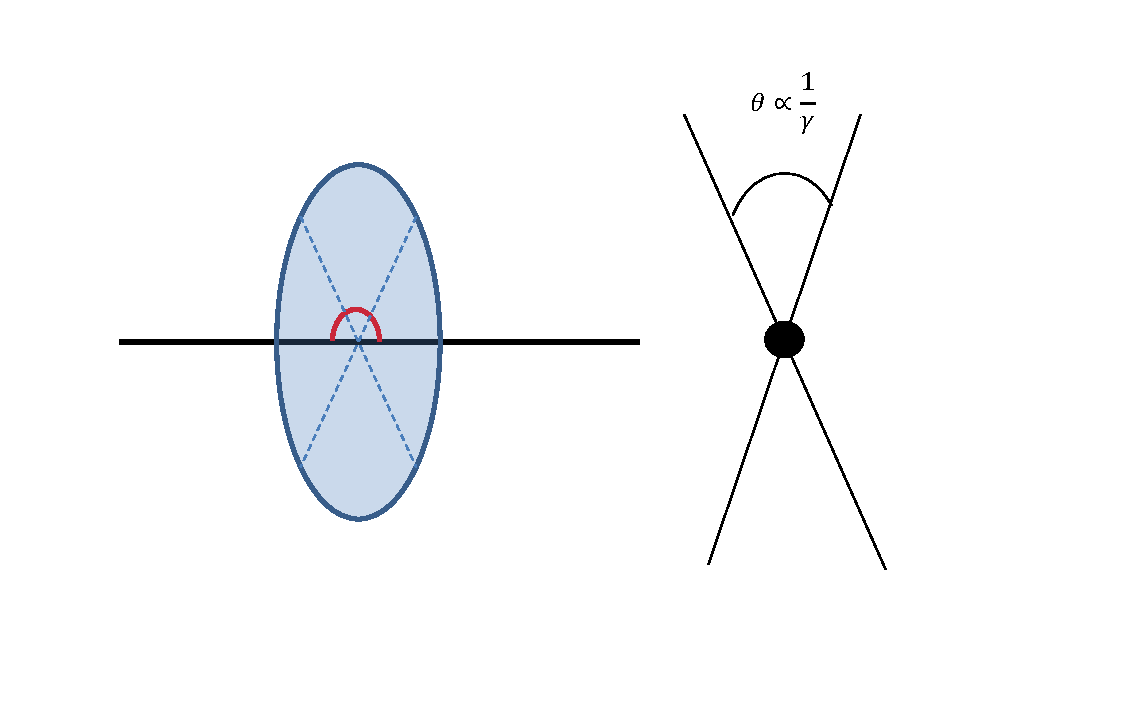
\includegraphics[width=0.6\textwidth]{Bench_Top_Measurements/figures/coaxial-particle-fields.pdf}
\end{center}
\caption{Comparison of the electromagnetic field profile of a moving charged particle and a short time pulse propagating along a coaxial wire.}
\label{fig:coax-part-profile}
\end{figure}

\subsection{Classical Coaxial Wire Method}

The classical coaxial wire method, first proposed in it's present form by V. Vaccarro in 1990 \cite{Vaccaro:ImprovedWireMeth}, is a transmission method that measures the complex transmission coefficient of a DUT (Device Under Test) made up of the equipment whose impedance is to be measured and a coaxial wire passing through it. 

The experimental setup is as shown in Fig. \ref{fig:classic-coax}. Firstly the external circuit (i.e. everything which is not the DUT such as VNA, cables, transition between connections etc.) is matched to the characteristic impedance of the coaxial line inside the DUT. This is done by measuring the reflection coefficient $\Gamma$ for the setup with only one port connected to the DUT and the other end terminated by an open connection. Knowing the characteristic impedance of the VNA and associated cables (typically $Z_{c0} = 50\Omega$), we can easily calculate the characteristic impedance of the DUT, $Z_{c}$, from the relation,

\begin{equation}
\Gamma = \frac{Z_{c} - Z_{c0}}{Z_{c} + Z_{c0}}.
\end{equation}

It is then possible to electrically match the characteristic impedance by adding a resistive network between the DUT and the external circuit. This may be done in two ways:

\begin{enumerate}
\item{Adding resistors in series just before the DUT to resistively match the characteristic impedance (as seen by the DUT) of the VNA and associated measurement setup to that of the DUT, such that the series resistance $R_{s}=Z_{c0}-Z_{0}$. Often an attenuator is used to reduce the effect of reflections from the mismatch between the VNA and the resistor, shown in Fig.~\ref{fig:resMatch}.}
\item{The use of two way matching, using a parallel ($R_{p}$) and series ($R_{s}$) resistor, as shown in Fig.~\ref{fig:twoWayMatch}. The values for these resistances are given by}
\begin{align}
R_{p} = Z_{c0}\frac{\sqrt{Z_{c0}}}{Z_{c0}-Z_{0}} \nonumber \\
R_{s} = Z_{c0} - \frac{Z_{c0}R_{p}}{Z_{c0}+R_{p}} \nonumber
\end{align}
\end{enumerate} 

\begin{figure}
\subfigure[]{
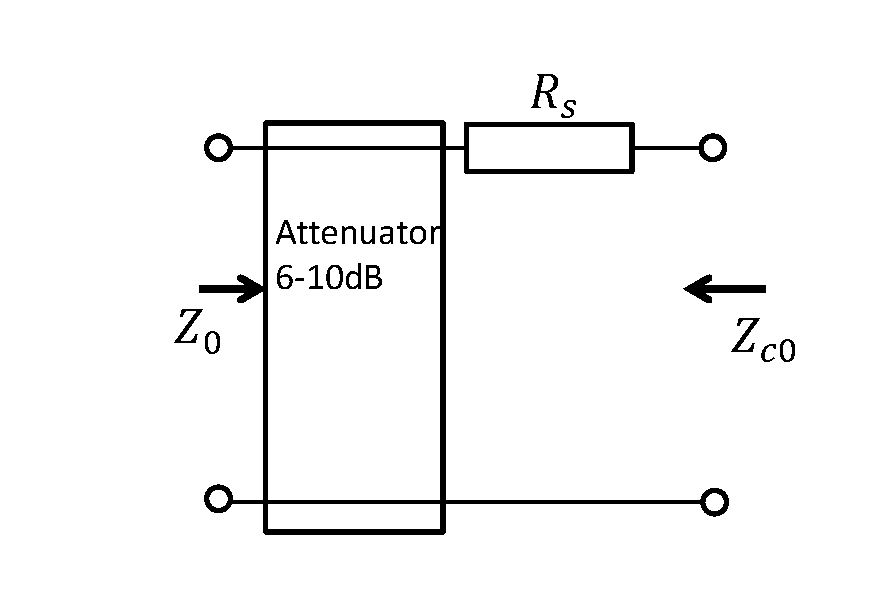
\includegraphics[width=0.45\textwidth]{Bench_Top_Measurements/figures/matching1Way.pdf}
\label{fig:resMatch}
}
\subfigure[]{
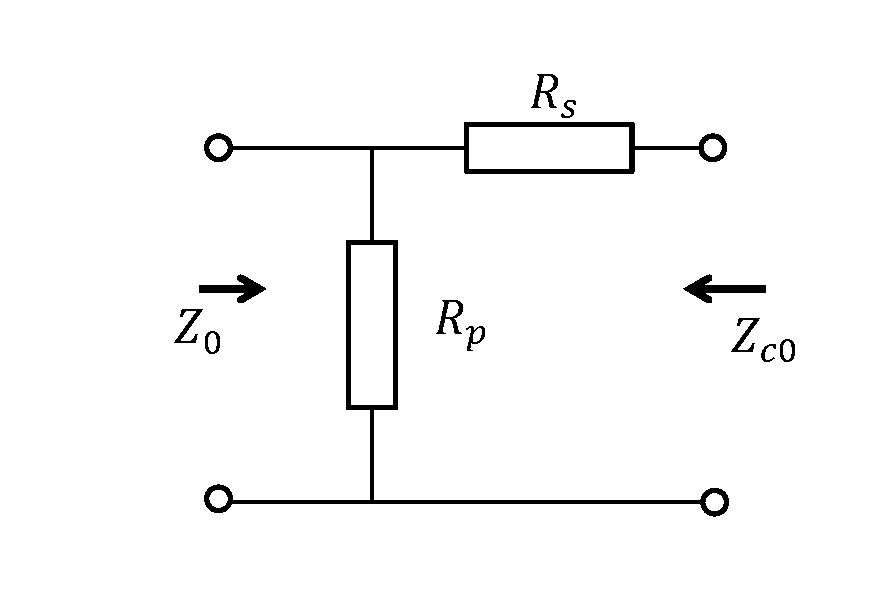
\includegraphics[width=0.45\textwidth]{Bench_Top_Measurements/figures/matching2Way.pdf}
\label{fig:twoWayMatch}
}
\caption{The resistive networks for matching a DUT to the attached measuring network (VNA and connecting cables). \subref{fig:resMatch} shows series resistive matching and \subref{fig:twoWayMatch} shows a two way matching network.}
\end{figure}

It is possible to use physical matching also using transition cones but these are costly, time consuming to construct, work only for a restricted frequency range and require new cones for each piece of equipment measured. And as can be seen in Fig. \ref{fig:matching-plot}, matching with a resistor is highly effective at removing the presence of reflections in coaxial measurements.

\begin{figure}
\begin{center}
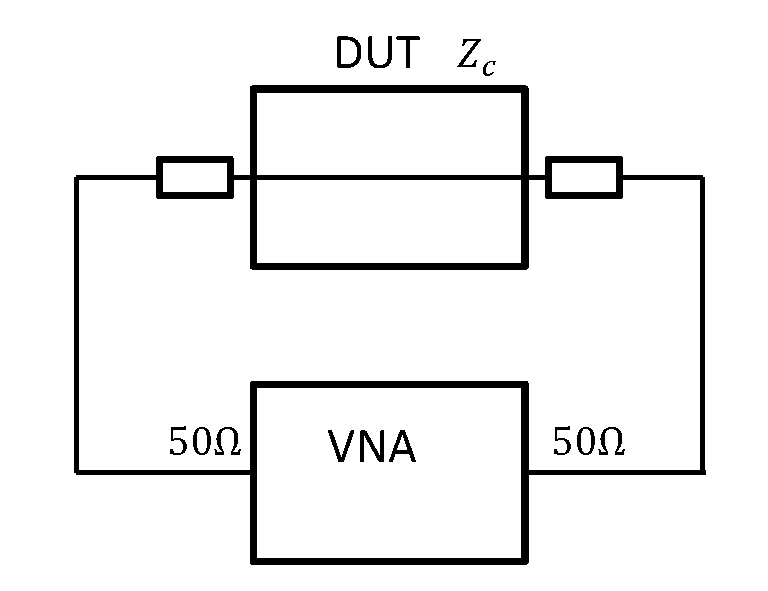
\includegraphics[width=0.6\textwidth]{Bench_Top_Measurements/figures/wire_meas_single_wire.pdf}
\end{center}
\caption{Experimental setup for a measurement of the beam coupling impedance using the classical coaxial wire method.}
\label{fig:classic-coax}
\end{figure} 

\begin{figure}
\begin{center}
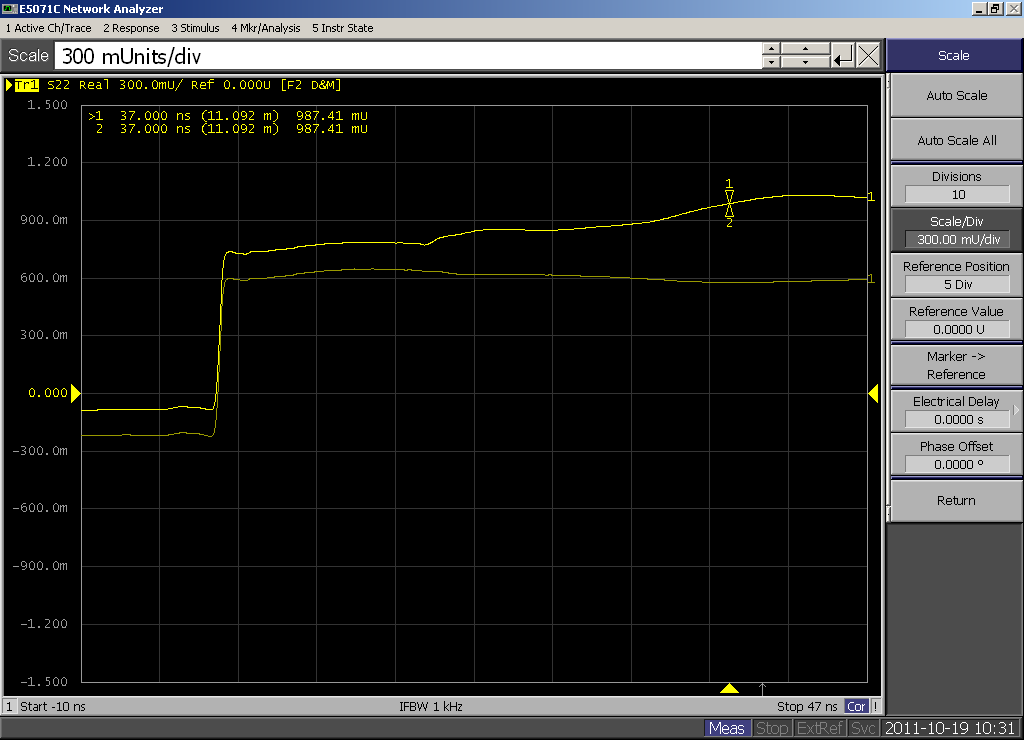
\includegraphics[width=0.6\textwidth]{Bench_Top_Measurements/figures/coax-matching-no-matching.png}
\end{center}
\caption{An example of a reflection measurement made with and without matching resistors. The faded line (lower trace) is the measurement with matching, the bold line (upper trace) that without. The reduction in the reflection can be seen due to the flatter line after the initial reflection.}
\label{fig:matching-plot}
\end{figure}

The values that we wish to measure to evaluate the beam coupling impedance of a device are the scattering parameters of the resulting circuit, in particular $S_{21}$, the normalised transmission parameter through the DUT. $S_{21}$ is calculated by taking the measured transmission parameter $S_{21,DUT}$ and dividing it by the transmission parameter through a reference line of the same physical length as the DUT,

\begin{equation}
S_{21} = \frac{S_{21,DUT}}{S_{21,REF}}.
\end{equation}

The effect of this is to correct the measured phase change in the DUT to be that only caused by the imaginary component of the beam coupling impedance.

There are subsequently a number of ways to evaluate the beam coupling impedance of the DUT depending on it's expected properties. For devices that are expected to have either a small impedance, or those that are physically very short in length, it is possible to use the so called lumped impedance formula \cite{Hahn:BenchMeasInter, Hahn:ValidityImpMeas};

\begin{equation}
Z = 2Z_{c} \frac{1-S_{21}}{S_{21}}.
\end{equation}

For distributed impedances, it is suitable to use the so called log formula (called so due to the exponential attenuation of the signal causing a log function to appear in the evaluation) \cite{Hahn:BenchMeasInter, Hahn:ValidityImpMeas, Jensen:ImprovLogForm},

\begin{equation}
Z = -2Z_{c} ln \left( S_{21} \right).
\end{equation}

For long components or measurements at very high frequencies there exists the improved log formula. This takes into account more completely the electrical length of the device, given by

\begin{equation}
Z = -2Z_{c} ln \left( S_{21}  \right) \left( 1 + j\frac{ln \left( S_{21}\right) }{2\Theta}  \right)
\end{equation}

where $\Theta = 2\pi \frac{L}{\lambda}$ is the normalised electrical length of the device, $L$ the length of the device. It is possible to see that the lumped impedance formula can be used when $\Theta \leq 1$, and the improved log formula becomes useful for $\Theta \geq 5$ \cite{Jensen:ImprovLogForm}.




\subsection{Resonator Coaxial Wire Method}
\label{sec:reson-coax-meth}

An alternative method for measuring the beam coupling impedance is by using the so called resonator method. The setup for this method is similar to that of the classical coaxial wire method, except that the matching resistor network between the VNA and DUT is replaced by a weak capacitive coupling ($S_{11} < 0.5dB$, remembering that $0dB$ means full reflection, i.e. no coupling) at both ends of the DUT. This then produces a structure which resonates at frequencies where the wavelength corresponds to the classical closed structure form,

\begin{equation}
\lambda = \frac{2L}{n}
\end{equation}

where $\lambda$ is the wavelength of the resonance, $n$ the harmonic of the resonance and $L$ the length of the device. 

The resonant method enables accurate measurement of the transmission losses due to the real longitudinal impedance. Additional advantages are that no matching is required, and a large number of mechanical uncertainties (electrical connections, consistency of calibration) can be avoided. However it can be seen that the frequency resolution is limited due to the length of the DUT so the method is not recommended as the only measurement method for structures expected to contain high-Q, narrowband resonances. It can however be used to corroborate the results obtained using the classical method.

For each resonant peak, the loaded Q-factor and the frequency of the resonance are measured. For a weak coupling at both ends of the DUT, we can write the coupling coefficient $k$ as

\begin{equation}
k = \frac{\left| S_{21} \right|}{1 - \left| S_{21} \right| }.
\label{eqn:coupling_coeff}
\end{equation}

The difference between the unloaded $Q$-factor, $Q_{0}$ , and the loaded $Q$-factor, $Q_{L}$, is a function of $k$. The loaded Q is the Q of the DUT resonance coupled with the measurement circuitry, and the unloaded Q the Q of the DUT resonance in isolation. We can get an approximate correction by using the formula

\begin{equation}
Q_{0} = Q_{L} \left( 1 + k  \right).
\label{eqn:Q_correc}
\end{equation}

Subsequently the measured line attenuation (in Np/m) is then calculated

\begin{equation}
\alpha_{m} = \frac{\pi}{\lambda Q_{0}}.
\label{eqn:atten}
\end{equation}

Note that this attenuation includes both that from the beam coupling impedance as well as that due to the finite resistance of the wire material. We can estimate the attenuation due to the wire material as

\begin{equation}
\alpha_{w} = \sqrt{\pi \rho_{w} \epsilon f} \frac{1}{d ln D/d}
\label{eqn:wire_atten}
\end{equation}

where $\rho_{w}$ is the wire resistivity, $\epsilon$ the wire permitivitty, $f$ the frequency, $d$ the diameter of the inner conductor and $D$ the diameter of the outer conductor (typically the vacuum beam pipe diameter). At very low frequencies the finite skin depth of the inner conductor would also have to be taken into account. Using the corrected attentuation $\alpha = \alpha_{m} - \alpha_{w}$, the real longitudinal impedance per unit length can be found to be 

\begin{equation}
\Re e\left\{ Z \right\} = 2Z_{c} \alpha
\label{eqn:res_imp}
\end{equation}

\begin{figure}
\begin{center}
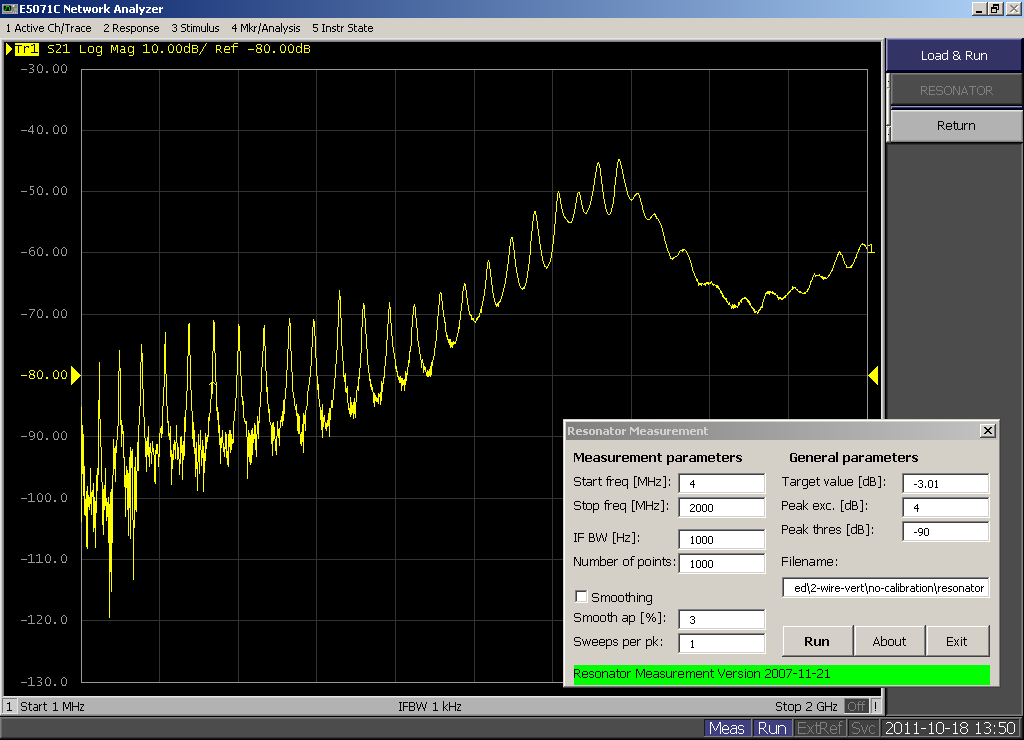
\includegraphics[width=0.6\textwidth]{Bench_Top_Measurements/figures/coax-resonator.png}
\end{center}
\caption{An example of the resonance pattern seen whilst performing measurements using the resonant method. Each peak corresponds to one data point in the final measurements. Taken from measurements of the LHC injection kicker magnets.}
\label{fig:res-resonancce-examples}
\end{figure}

It is more involved to calculate the imaginary impedance using the resonant method. In particular it is necessary to calculate the resonant frequencies of a pipe open at both ends of the same length of the DUT made of a good conducting material (i.e. the physical length is equal to the electrical length). This allows the comparison to the measured resonant frequencies of the DUT, the difference between which is dependent on the imaginary impedance.

Considering the complex impedance of the two measurements, $Z_{DUT}$ for the DUT and $Z_{REF}$ for a perfectly conducting reference pipe, they can be written as

\begin{align}
Z_{DUT} & =  R + jX_{1}  =  Z_{1}e^{j \phi} \\
Z_{REF} & =  jX_{2}  =  Z_{2}e^{j.0}
\end{align}

where $R$ is the resistive component of the DUT impedance, $X_{1/2}$ the imaginary component of the impedance (DUT and reference pipe respectively), $\phi$ is the angle of DUT impedance projected onto a complex plane and $Z_{2} = \sqrt{R^{2} + X^{2}}$. If we consider a measured value depedent on the impedance, for example the transmission parameter $S_{21}$ at a resonant peak, we have the following relations

\begin{align}
S_{21}^{DUT} = S_{0}e^{j \left( \omega_{1}t + \phi \right)} \\
S_{21}^{REF} = S_{0}e^{k \left( \omega_{2}t \right)}
\end{align}

where $S_{0}$ is some normalised scalar, $\omega_{1/2}$ is the frequency of the resonance and $t = \frac{L}{c}$ . Thus for a pair of corresponding peaks from resonance measurements for which we have measured $\omega_{1}$ and $\omega_{2}$ we can equate $S_{21}^{DUT} = S_{21}^{REF}$ and thus show

\begin{equation}
\phi = t \left( \omega_{2} - \omega_{1} \right).
\end{equation}

Subsequently we can see that

\begin{equation}
X = Z_{DUT} sin \phi = R \frac {sin \phi}{cos \phi} = R tan \phi
\end{equation}

where $R = \Re e(Z)$.

\subsection{Transverse Impedance Measurements}

The above methods give a general impression of how to carry out coaxial wire measurements of the impedance of accelerator components. Directly applied as described they allow the measurement of the longitudinal impedance of a DUT. However, from a beam stability point of view, it is also interesting to look at the transverse impedance of a device. In particular it would be useful to have a method of determining the vertical/horizontal dipolar (or driving) impedance and the vertical/horizontal quadrupolar (detuning) impedance of any device. In this section we describe how to do this for structures with top/bottom, left/right symmetry and then generalise to asymmetric structures, with illustration from simple examples evaluated using simulations.

To allow a complete explanation of how to verify the methods of measuring transverse impedances, let us first consider the general form of the $m$-th order ($m = 0, 1, 2,...$) longitudinal beam coupling impedance, given by \cite{Chao:PhysColEff, Tsutsui:OnSingleWire}

\begin{equation}
\bar{Z}_{m} = \frac{-1}{I^{2}} \int dV \mathbf{\bar{E}_{m}. \bar{J}_{m}^{*}}
\end{equation}

where $\bar{J}_{m}$ is the current density of the source. For a beam propogating along the z-axis with an offset $a$ and moment $cos \left( m \theta \right)$,

\begin{equation}
\mathbf{\bar{J}_{m}} = \frac{I}{\pi a^{m +1} \left( 1 + \delta_{m0} \right)} \delta \left( r - a \right) cos \left( m \theta \right) exp \left( j \left( \omega t - k z  \right) \right) \mathbf{e_{z}}.
\end{equation}

The electromagnetic field associated with a given current source $\mathbf{\bar{J}_{m}}$ is $\left( \mathbf{\bar{E}_{m}}, \mathbf{\bar{H}_{m}} \right)$. 

It can be seen that any different azimuthal components of the $m$-th field of order $n$ (i.e. $sin \left( n\theta \right)$ and $cos \left( n\theta \right)$ terms) are neglected in this treatment. To allow the treatment of coupling between different azimuthal orders we can define a longitudinal beam coupling impedance $Z_{m,n}$ (where $m,n = 0, \pm 1, \pm 2, ... $)

\begin{equation}
Z_{m,n} = \frac{-1}{I^{2}} \int dV \mathbf{E_{m}. J_{n}^{*}}
\end{equation}

where

\begin{equation}
\mathbf{J_{m}} = \frac{I}{2 \pi a^{|m |+1}} \delta \left( r - a \right) exp \left(j m \theta \right) exp \left( j \left( \omega t - k z  \right) \right) \mathbf{e_{z}}.
\end{equation}

Importantly, this allows us to see that 

\begin{align}
\mathbf{\bar{J}_{0}} &= \mathbf{J_{0}} \nonumber \\
\mathbf{\bar{J}_{m}} &= \mathbf{J_{m}} + \mathbf{J_{-m}}.
\end{align}

From here we use the principle of superposition for electromagnetic fields (i.e. we neglect any non-linearities of the surrounding materials), and thus can derive

\begin{align}
\bar{Z}_{0} &= Z_{0} \\
\bar{Z}_{x} &= \bar{Z}_{1} = Z_{1,1} + Z_{1,-1} + Z_{-1,1} + Z_{-1,-1} = kZ^{dip}_{x}\\
\bar{Z}_{x} &= \bar{Z}_{1} \text{(cos replaced with sin)}= Z_{1,1} - Z_{1,-1} - Z_{-1,1} + Z_{-1,-1} = kZ^{dip}_{y}\\
\bar{Z}_{m} &= Z_{m,m} + Z_{m,-m} + Z_{-m,m} + Z_{-m,-m}, m=1,2,...
\end{align}

From this start we will apply this to both two wire measurements and to displaced single wire measurements.

\subsubsection{Two Wire Measurements}

It is possible to directly measure the dipolar impedance of a device through the use of a two wire coaxial method. The measurement setup is identical to that of the single wire method, except that two wires, seperated by distance $\Delta$, are placed in the device, and a 180$^{\circ}$ hybrid is place between the wires and the VNA at both ends of the device. This setup is illustrated in Fig. \ref{fig:two_wire_measure}

\begin{figure}
\begin{center}
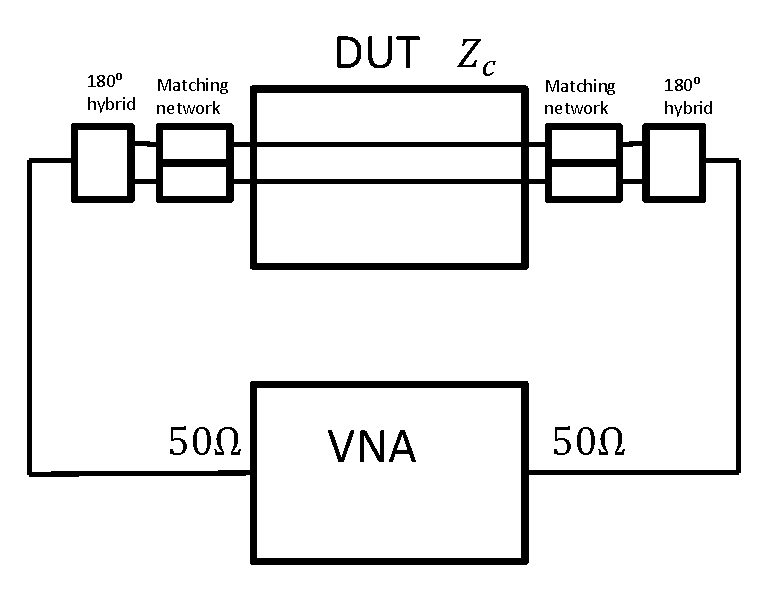
\includegraphics[width=0.6\textwidth]{Bench_Top_Measurements/figures/wire_meas_two_wire.pdf}
\end{center}
\caption{Measurement setup for measurements of the dipolar beam coupling impedance using the two wire setup for the classical coaxial wire method.}
\label{fig:two_wire_measure}
\end{figure}

The measurements are done in the same way as described in the previous sections for either the classical transmission method or the resonator method. When using the classical coaxial wire method, both wires are individually matched to $Z_{c0}$. By using two wires each carrying a signal 180$^{o}$ out of phase with one another we produce a field pattern similar to a dipole and thus measure the dipole impedance in either the horizontal or vertical plane depending on the orientation of the two wires. 

What is directly measured is the longitudinal impedance of just the dipole impedance, as is to be expected from the Panofsky-Wenzel theorem (see Sec.~\ref{sec:PanWen} for further explanation). 

For two wire placed at positions $x = \pm a$ relative to the centre of the aperture, the source current density is given by \cite{Tsutsui:OnSingleWire}

\begin{align}
J & =  I \left( \delta \left( x - a \right) - \delta \left( x + a  \right) \right) \delta (y) exp \left( j \left( \omega t - kz \right) \right) \nonumber \\
& =  \frac{I}{\pi a} \displaystyle\sum\limits_{m=-\infty}^{\infty} exp \left(j \left( 2m +1 \right) \theta \right) exp \left( j \left( \omega t - kz \right) \right) \nonumber \\
& =  2\displaystyle\sum\limits_{m=-\infty}^{\infty} a^{|2m + 1 |} J_{2m + 1}.
\end{align}

The impedance is then

\begin{align}
Z & =  - \frac{1}{I^{2}} \int dV \left( 2\displaystyle\sum\limits_{m=-\infty}^{\infty} a^{|2m + 1 |} E_{2m + 1}  \right)  \left( 2\displaystyle\sum\limits_{n=-\infty}^{\infty} a^{|2n + 1 |} J_{2n + 1}^{*}  \right) \nonumber \\
& =  4 \displaystyle\sum\limits_{m,n} a^{|2m + 1 | + |2n + 1|} Z_{2m + 1, 2n+1} \nonumber \\
& =  \left(2a \right)^{2}\left( Z_{1,1} + Z_{-1,1} + Z_{1,-1} + Z_{-1,-1} \right) + O(a^{4}) \nonumber \\
& =  (2a)^{2}\bar{Z}_{x} + O(a^{4}). 
\end{align}

Again using the Panofsky-Wenzel theorem we can deduce that the transverse dipolar impedance $Z^{dip}_{x/y}$ is given by 

\begin{equation}
Z^{dip}_{x/y} = \frac{\bar{Z}_{x/y}}{k} = \frac{c}{\omega} \frac{Z}{\Delta^{2}}
\end{equation}

where $\Delta = 2a$ and $Z$ is the measured complex impedance.

\subsubsection{Structures with Top/Bottom, Left/Right Symmetry}

If we consider a source particle at $x_{1} = a_{1}cos\theta_{1}, y_{1} = a_{1}sin\theta_{1}$ and a test particle at $x_{2} = a_{2}cos\theta_{2}, y_{2} = a_{2}sin\theta_{2}$, the source current density is

\begin{align}
J_{z} &= I\delta \left( x-x_{1} \right) \delta \left( y-y_{1} \right) exp \left( k \left( \omega t - kz \right) \right) \nonumber \\
          &=\displaystyle\sum\limits_{m=-\infty}^{\infty}a_{1}^{|m|}exp\left( -jm\theta_{1} \right) J_{m}
\end{align}

The impedance would therefore be

\begin{align}
Z = &\frac{-1}{I^{2}} \int dV \left( \displaystyle\sum\limits^{\infty}_{m=-\infty} a_{1}^{|m|} exp \left( jm\theta_{1} \right) E_{m}\right) \left( \displaystyle\sum\limits^{\infty}_{n=-\infty} a_{1}^{|n|} exp \left( jn\theta_{2} \right) J^{*}_{n}\right) \nonumber \\
   = &\displaystyle\sum\limits^{\infty}_{m,n=-\infty} a_{1}^{|m|} a_{2}^{|n|} exp\left( -jm\theta_{1} \right) exp\left( -jn\theta_{2} \right) Z_{m,n} \nonumber \\
   = &Z_{0,0} + \left( x_{1}- jy_{1} \right)Z_{1,0} + \left( x_{1} + jy_{1} \right)Z_{-1,0} + \left( x_{2} + jy_{2} \right)Z_{0,1} +  \left( x_{2} - jy_{2} \right)Z_{0,-1} \nonumber \\
      & +\left( x_{1} - jy_{1} \right)^{2}Z_{2,0} +  \left( x_{1} - jy_{1} \right)\left( x_{2} - jy_{2} \right)Z_{1,-1} + \left( x_{2} - jy_{2} \right) Z_{0,-2} \nonumber \\
      & +\left( x_{1} - jy_{1} \right)\left( x_{2} + jy_{2} \right)Z_{1,1} + \left( x_{1} + jy_{1} \right) \left( x_{2} - jy_{2} \right) Z_{-1,-1} \nonumber \\
      & +\left( x_{1} + jy_{1} \right)^{2}Z_{-2,0} + \left( x_{1} + jy_{1} \right)\left( x_{2} - jy_{2} \right) Z_{-1,1} + \left( x_{2} - jy_{2} \right)^{2}Z_{0,2} \nonumber \\
      & +O\left( \left(  x_{1},y_{1},x_{2},y_{2} \right)^{3} \right).
\label{eqn:gen_imp}
\end{align}

By applying Panofsky-Wenzel we see that

\begin{align}
kZ_{x} =\frac{\partial Z}{\partial x_{2}} = & Z_{0,1} + Z_{0,-1} + \left( x_{1} - jy_{1} \right) Z_{1,-1} + 2\left( x_{2} - jy_{2} \right) Z_{0,-2} \nonumber \\
						&+ \left( x_{1} - jy_{1} \right) Z_{1,1} + \left( x_{1} + jy_{1} \right) Z_{-1,-1} + \left( x_{1} + jy_{1} \right) Z_{-1,1} + 2\left( x_{2} + jy_{2} \right) Z_{0,2} \nonumber \\
						& + O\left( \left( x_{1},y_{1},x_{2},y_{2} \right)^{2} \right) \nonumber \\
						= & Z_{0,1} + Z_{0,-1} + x_{1}\bar{Z}_{x} + jy_{1} \left( -Z_{1,-1} - Z_{1,1} + Z_{-1,-1} + Z_{-1,1} \right) \nonumber \\
						& + x_{2}\left( 2Z_{0,-2} + 2Z_{0,2}  \right) + jy_{2}\left( -2Z_{0,-2} + 2Z_{0,2}  \right) +  O\left( \left( x_{1},y_{1},x_{2},y_{2} \right)^{2} \right)
\end{align}

\begin{align}
kZ_{y} =\frac{\partial Z}{\partial y_{2}} = & jZ_{0,1} - jZ_{0,-1} - j\left( x_{1} - jy_{1} \right) Z_{1,-1} - 2j\left( x_{2} - jy_{2} \right) Z_{0,-2} \nonumber \\
						&+ j\left( x_{1} - jy_{1} \right) Z_{1,1} - j\left( x_{1} + jy_{1} \right) Z_{-1,-1} + j\left( x_{1} + jy_{1} \right) Z_{-1,1} + 2j\left( x_{2} + jy_{2} \right) Z_{0,2} \nonumber \\
						& + O\left( \left( x_{1},y_{1},x_{2},y_{2} \right)^{2} \right) \nonumber \\
						= & j\left(Z_{0,1} - Z_{0,-1} \right)+ y_{1}\bar{Z}_{y} + jx_{1} \left( -Z_{1,-1} + Z_{1,1} + Z_{-1,-1} + Z_{-1,1} \right) \nonumber \\
						& + y_{2}\left(- 2Z_{0,-2} - 2Z_{0,2}  \right) + jx_{2}\left( -2Z_{0,-2} + 2Z_{0,2}  \right) +  O\left( \left( x_{1},y_{1},x_{2},y_{2} \right)^{2} \right).
\end{align}

Two properties to note for later use are that

\begin{align}
\textbf{J}_{-m} \left( \omega \right) & = \textbf{J}_{m}^{*} \left( -\omega \right) \\
Z_{-m,-n} \left( \omega \right) & = Z_{m,n}^{*} \left( -\omega \right).
\end{align}

If we now assume a single wire rather than a source and test particle, such that $x_{1}=x_{2}=x_{0}, y_{1}=y_{2}=y_{0}$. This gives a source current density

\begin{align}
J & = I \delta \left( x-x_{0} \right)\delta \left( y-y_{0} \right) exp\left( j \left(\omega t -kz \right)\right) \nonumber \\
  & = \frac{I}{2\pi a} \delta \left( r-a \right)\displaystyle\sum\limits_{m=-\infty}^{\infty} exp\left( jm \left( \theta -\theta_{0} \right) \right) exp\left( jm \left( \theta -\theta_{0} \right) \right) exp\left( j \left( \omega t - kz \right) \right) \nonumber \\
  & = \displaystyle\sum\limits_{m=-\infty}^{\infty} a^{|m|}exp\left( -jm\theta_{0} \right)J_{m}.
\end{align}

We can then define $x_{0}=acos\theta_{0}, y_{0}=asin\theta_{0}$. Entering this into Eqn. \ref{eqn:gen_imp} gives

\begin{align}
Z &=&Z_{0,0} +  \left( x_{0} - jy_{0} \right) Z_{1,0} + \left( x_{0} + jy_{0} \right)  Z_{-1,0} + \left( x_{0} + jy_{0} \right) Z_{0,1} \nonumber \\
   &   &+ \left( x_{0} - jy_{0} \right) Z_{0,-1} + \left( x_{0} - jy_{0} \right)^{2} Z_{2,0} + \left( x_{0} - jy_{0} \right)^{2} Z_{1,-1} + \left( x_{0} - jy_{0} \right) ^{2}Z_{0,-2} \nonumber \\
   &   &+\left( x_{0} - jy_{0} \right) \left( x_{0} + jy_{0} \right) Z_{1,1} + \left( x_{0} + jy_{0} \right)\left( x_{0} - jy_{0} \right) Z_{-1,-1} + \left( x_{0} + jy_{0} \right)^{2}Z_{-2,0} \nonumber \\
   &   &+\left( x_{0} + jy_{0} \right)^{2} Z_{-1,1} + \left( x_{0} + jy_{0} \right)^{2}Z_{0,2} + O\left( \left(x_{0},y_{0} \right)^{2} \right) \nonumber \\
   &=&Z_{0,0} + x_{0}\left( Z_{1,0}+Z_{-1,0}+Z_{0,1}+Z_{0,-1} \right) +jy_{0} \left( -Z_{-1,0} + Z_{-1,0} + Z_{0,1} - Z_{0,-1} \right) \nonumber \\
   &   &+x_{0}^{2} \left(  Z_{1,-1}+Z_{1,1}+Z_{-1,-1}+Z_{-1,1} + Z_{2,0} + Z_{0,-2} + Z_{0,2} + Z_{-2,0} \right) \nonumber \\
   &   &+y_{0}^{2} \left(  -Z_{1,-1}+Z_{1,1}+Z_{-1,-1}-Z_{-1,1} - Z_{2,0} - Z_{0,-2} - Z_{0,2} - Z_{-2,0} \right) \nonumber \\
   &   &+2jx_{0}y_{0}\left( -Z_{2,0} - Z_{0,-2} + Z_{-2,0} + Z_{0,2} + Z_{-1,1} - Z_{1,-1} \right) \nonumber \\
   &=&Z_{0,0} + x_{0}\left( Z_{1,0}+Z_{-1,0}+Z_{0,1}+Z_{0,-1} \right) +jy_{0} \left( -Z_{-1,0} + Z_{-1,0} + Z_{0,1} - Z_{0,-1} \right) \nonumber \\
   &   &+x_{0}^{2} \left( \bar{Z}_{x} + Z_{2,0} + Z_{0,-2} + Z_{0,2} + Z_{-2,0} \right) \nonumber \\
   &   &+y_{0}^{2} \left( \bar{Z}_{y} - Z_{2,0} - Z_{0,-2} - Z_{0,2} - Z_{-2,0} \right) \nonumber \\
   &   &+2jx_{0}y_{0}\left( -Z_{2,0} - Z_{0,-2} + Z_{-2,0} + Z_{0,2} + Z_{-1,1} - Z_{1,-1} \right).
\label{eqn:gen_single_wire}
\end{align}

It can then be seen that if measurements are made with $x_{0} = 0$ and taking different values of $y_{0}$ that one obtains data with a parabolic fit in the $y_{0}$ axis. By fitting a curve to this we obtain constant (equal to the longitudinal impedance), linear and quadratic terms. Doing the same for $y_{0}=0$ allows us to derive two quadratic terms

\begin{align}
Z^{\perp}_{x} & = \left( \bar{Z}_{x} + kZ_{quad} \right)\frac{1}{k} =  Z^{dip}_{x} + Z_{quad}\\
Z^{\perp}_{y} & = \left( \bar{Z}_{y} - kZ_{quad} \right)\frac{1}{k}= Z^{dip}_{y} - Z_{quad} \\
\end{align}

where $Z_{quad}=\frac{1}{k}\left( Z_{0,2}+Z_{2,0}+Z_{0,-2}+Z_{-2,0}  \right) = \frac{2}{k}\left( Z_{0,2}+Z_{0,-2}  \right)$ (shown in the case of 2D structures externally bounded by a perfectly conducting boundary in \cite{Tsutsui:OnSingleWire}), representing the impedance due to the displacement of the test particle in an accelerator. As we can measure $\bar{Z}_{x/y}$ independently using the two wire method we can thus indepedently measure $Z_{quad}$ using a displaced single wire scan in both the x- and y-planes.

It can also be seen that

\begin{align}
Z^{\perp}_{x} + Z^{\perp}_{y} = \frac{1}{k}\left( \bar{Z}_{x} + \bar{Z}_{y} \right) = Z^{dip}_{x} + Z^{dip}_{y}
\end{align}

where $\bar{Z}_{x/y}$ can be measured independently which gives a method of obtaining confidence in the wire measurements.

\subsubsection{Asymmetric Structures}

If Eqn. \ref{eqn:gen_single_wire} is transformed from $\left( x,y \right)$ coordinates to $\left( a, \theta \right)$, the result is

\begin{align}
Z &=Z_{0,0} +a\left[ cos\theta \left( Z_{-1,0} + Z_{0,1} \right) +jsin\theta \left( Z_{-1,0} + Z_{0,1} \right)  cos\theta \left( Z_{1,0} + Z_{0,-1} \right) - jsin\theta \left( Z_{1,0} + Z_{0,-1} \right)\right] \nonumber \\
   &+a^{2}\left[ cos^{2} \left( Z_{1,1} + Z_{-1,-1} \right) + sin^{2} \left( Z_{1,1} + Z_{-1,-1} \right)\right] \nonumber \\
   &+a^{2}\left[ cos^{2} \left( Z_{2,0} + Z_{0,-2} +Z_{1,-1} \right) +2jsin\theta cos\theta\left( Z_{2,0} + Z_{0,-2} +Z_{1,-1} \right) \right] \nonumber \\
   & - a^{2}\left[sin^{2} \left( Z_{2,0} + Z_{0,-2} +Z_{1,-1} \right)\right] \nonumber  \\
   &+ a^{2}\left[ cos^{2} \left( Z_{-2,0} + Z_{0,2} +Z_{-1,1} \right) +2jsin\theta cos\theta\left( Z_{-2,0} + Z_{0,2} +Z_{-1,1}  \right) \right] \nonumber \\
   &+ a^{2}\left[sin^{2} \left( Z_{-2,0} + Z_{0,2} +Z_{-1,1}  \right) \right].
\end{align}

Grouping terms by order of depedence on $a$ and $\theta$ this becomes
\begin{align}
Z   &=Z_{0,0} + a\left[ e^{-j\theta}\left( Z_{-1,0} + Z_{0,1} \right) +  e^{j\theta}\left( Z_{1,0} + Z_{-0,1} \right)\right] \nonumber \\
     &+a^{2}\left[ \left( Z_{1,1} + Z_{-1,-1} \right) + e^{-2j\theta} \left(  Z_{2,0} + Z_{0,-2} +Z_{1,-1} \right) + e^{2j\theta} \left( Z_{-2,0} + Z_{0,2} +Z_{-1,1} \right) \right] \nonumber \\
     &=A_{1} + ae^{-j\theta}A_{2} + ae^{-j\theta}A_{3}+ a^{2}e^{-2j\theta}A_{4} +a^{2}e^{2j\theta}A_{5} +  a^{2}A_{6}
\label{eqn:rot_gen}
\end{align}

where $A_{1} = Z_{0,0}$, $A_{2} = Z_{0,1}+Z_{-1,0}$, $A_{3} = Z_{0,-1}+Z_{1,0}$, $A_{4} = Z_{0,2}+Z_{-1,1}+Z_{-2,0}$, $A_{5} = Z_{2,0}+Z_{1,-1}+Z_{0,-2}$ and $A_{6}=Z_{1,1}+Z_{-1,-1}$. Taking the earlier definition of $Z_{quad}$ it can be deduced that

\begin{align}
Z_{quad} & = \left( A_{4}+A_{5}+A_{6} - \bar{Z}_{x} \right)\frac{1}{k} =\frac{ A_{4}+A_{5}+A_{6}}{k} - Z^{dip}_{x} \\  
	    & = \left( A_{4}+A_{5} - \frac{\bar{Z}_{x}- \bar{Z}_{y}}{2}\right)\frac{1}{k} =\frac{ A_{4}+A_{5}}{k} - \frac{Z^{dip}_{x}-Z^{dip}_{y} }{2}.
\end{align}

Consideration of Eqn. \ref{eqn:rot_gen} lets it be seen that

\begin{align}
 A_{4}+A_{5}+A_{6} & = \frac{Z\left( a,0 \right)+Z\left( a,\pi \right) - 2Z\left( 0,0 \right)}{2a^{2}} \\
 A_{4}+A_{5} & = \frac{Z\left( a,0 \right)+Z\left( a,\pi \right) - Z\left( a,\frac{\pi}{2} \right)-Z\left( a,\frac{3\pi}{2} \right)}{2a^{2}}.
\end{align}

The constant impedance can also be seen to be found by taking a linear fit of the longitudinal impedance of a wire displaced in either the $\theta = 0$ or $\theta = \pi / 2$ plane, and taking the linear term of the fit. 

\subsection{Measurements on Example Geometries}

In this section shall be presented a number of example analyses of coaxial wire measurements done on geometries exhibiting top/bottom, left/right symmetry and an asymmetric structure. This permits a step-by-step guide to analysis of the wire measurements, which may not be immediately clear from the mathematical introduction. These simulations are carried out using both Ansoft HFSS\cite{hfss} and Maxwell\cite{maxwell} using a driven modal solution. 

The simulations with HFSS are carried out in the following manner: for representing the single wire measurement the measurement system is simulated by placing waveguide ports at either end of the geometry with a conducting cylinder placed as the inner conductor of the coaxial system. The transmission parameters are then acquired as a result of the simulations. The wire may then be displaced as neccessary for the displaced single wire measurements. For two wire measurements a quarter geometry may be simulated, using a quarter geometry with a perfect H boundary in the plane of the wires, and a perfect E boundary between the wires to enforce the dipolar field pattern.

Maxwell is a frequency domain code optimised for low frequencies (less thans 10s of MHz). It does not permit the use of waveguide ports, however it does allow the definition of current segments with phase changes between them. By considering the current (either a single current segment to simulate a single wire, or two current carrying segments 180$^{\circ}$ out of phase for two wires) to be the equivalent of a beam current, and assuming the inclusion of the current carrying component is a negligible perturbation to the geometry, the real impedance can be found by summing the power loss in the system. This can be seen to be equivalent to the beam induced heating experienced by a beam interacting with an impedance.

This can be thought of by comparing the system to a homogenous transmission line. The power $P$ of a wave travelling along the line is given by \cite{Kroyer:lowFreqColImp}

\begin{equation}
P = P_{0}e^{-2\alpha z}
\end{equation}

where $P_{0}$ is the power at the beginning of the transmission line, $\alpha$ is the attenuation coefficient and $z$ the distance along the line. By differentiation it can be seen that

\begin{equation}
\alpha = -\frac{1}{2P} \frac{dP}{dz} \approx \frac{1}{2P} \frac{\delta P}{\delta z}
\end{equation}

where $\delta P$ is the power lost over the short distance $\delta z$. The transmission parameter of a line $S_{21}$ is given by

\begin{equation}
S_{21} = e^{-\alpha \delta z}.
\end{equation}

If the impedance is evaluated using the log formula ($Z = Z_{c}ln S_{21}$), it can be seen that the real impedance is subsequently given by

\begin{equation}
\Re{}e \left( Z \right) = Z_{c} \frac{2 \delta P}{P}.
\end{equation}

Assuming a peak current $I_{0}$ on the wire, $P = I_{0}^{2}Z_{c}/2$, which gives

\begin{equation}
\Re{}e \left( Z \right) = \frac{2 \delta P}{I_{0}^{2}}.
\end{equation}

To acquire the transverse impedance for two wire simulations it is simply neccesary to normalise by the wavenumber $k=\omega / c$ and the seperation of the wire $\Delta$ 

\begin{equation}
Z_{dip} = \frac{c}{\omega \Delta^{2}} \frac{2 \delta P}{I_{0}^{2}}.
\end{equation}

\subsubsection{Structure with Top/Bottom, Left/Rght Symmetry}

For the structure exhibiting top/bottom, left/right symmetry we use the Tsutsui model of two parallel plates as shown in Fig.~\ref{fig:tsutsui-model}. We use this due to the model allowing the prediction of the longitudinal, dipolar and quadrupolar impedances for a wide variety of materials and frequency ranges \cite{Tsutsui:ferrKickLong,Tsutsui:DipoleKicker, Salvant:QuadKicker}. For these simulations a short segment of a Tsutsui geometry is simulated using two different materials, in this case graphite, to represent a structure with a poor conductivity ($\sigma_{graphite} = 7 \times 10^{4} S m^{-1}$), and 4A4 ferrite, to represent a magnetically lossy material (in this case, $\epsilon_{r} = 10$, $\sigma_{4A4} = 10^{-6} S m^{-1}$ (a mild conductivity is applied to prevent static build up in ferrite components in accelerators), and $\mu_{r} = \mu^{'} + j \mu^{"}$, shown in Fig.~\ref{fig:4a4permeability}.). In both cases the following dimensions are used: $a=25mm$, $b=5mm$, $d=5mm$. A structure of 150mm in length is used to reduce numerical noise due to the small losses given by the short length of the simulated DUT.

\begin{figure}
\subfigure[]{
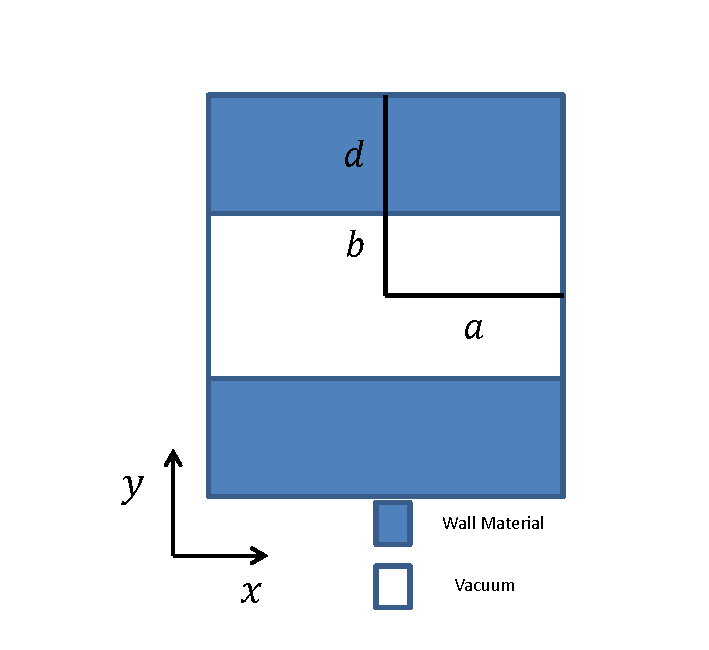
\includegraphics[width=0.45\textwidth]{Bench_Top_Measurements/figures/tsutsui-geometry.pdf}
\label{fig:tsutsui-model}
}
\subfigure[]{
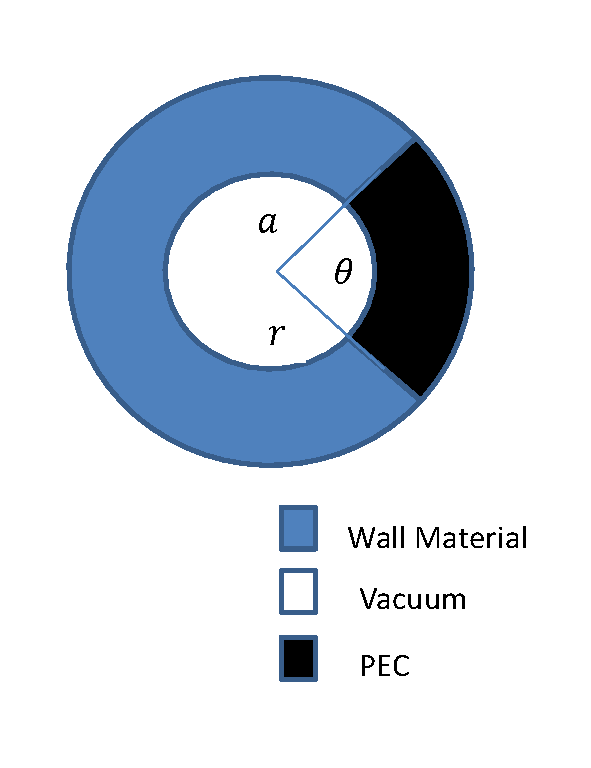
\includegraphics[width=0.45\textwidth]{Bench_Top_Measurements/figures/zannini-model-geo.pdf}
\label{fig:zannini-model}
}
\caption{The geometries used for coaxial wire measurement simulations. For the geometry with top/bottom, left/right symmetry we use the Tsutsui model (\subref{fig:tsutsui-model}) using two parallel plates. For the asymmetric structure we use the Zannini-model for a C-core ferrite kicker magnet (\subref{fig:zannini-model}), which generates a constant term and a noticeable asymmetric term.}
\label{fig:wire-measure-geometries}
\end{figure}

\begin{figure}
\begin{center}
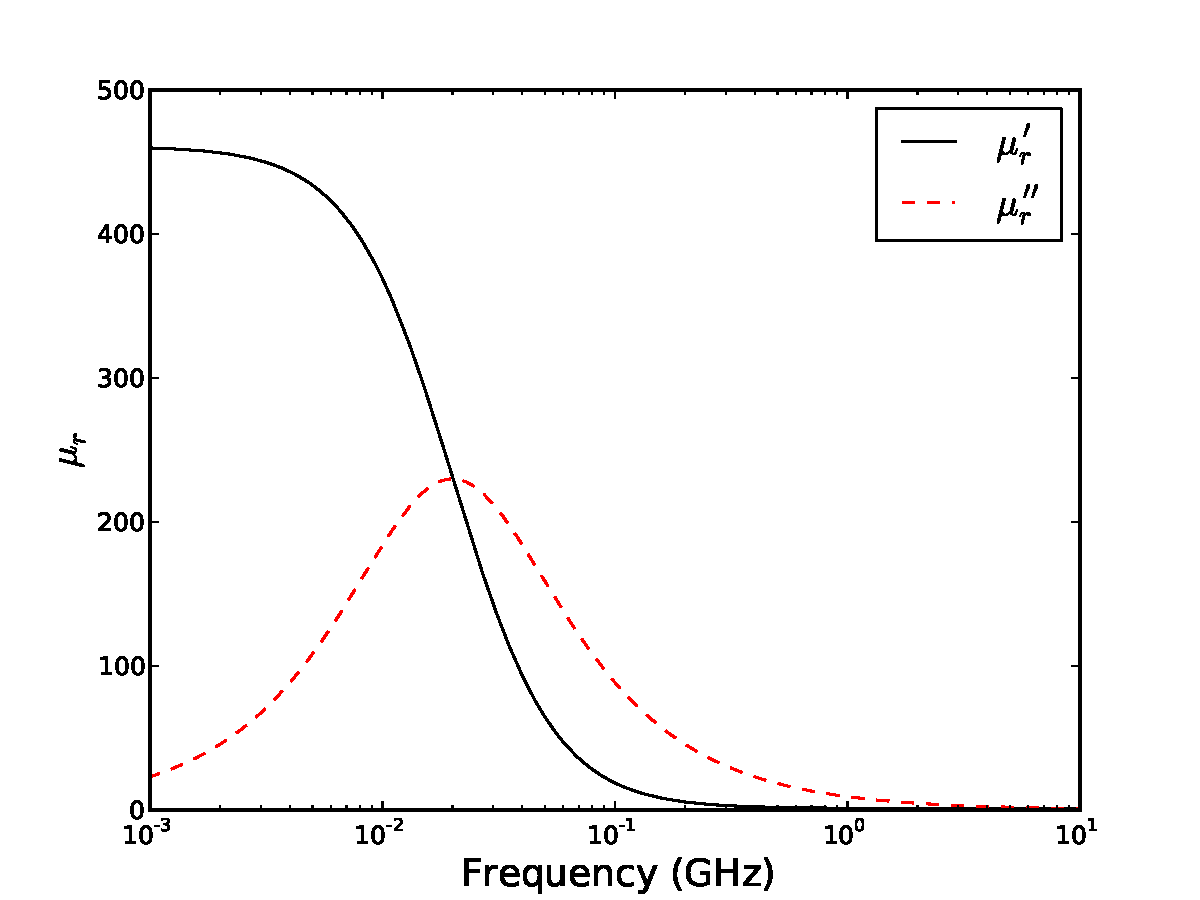
\includegraphics[width=0.45\textwidth]{Bench_Top_Measurements/figures/4A4FerrMu.pdf}
\end{center}
\caption{The complex permeability of 4A4 ferrite.}
\label{fig:4a4permeability}
\end{figure}

\begin{figure}
\begin{center}
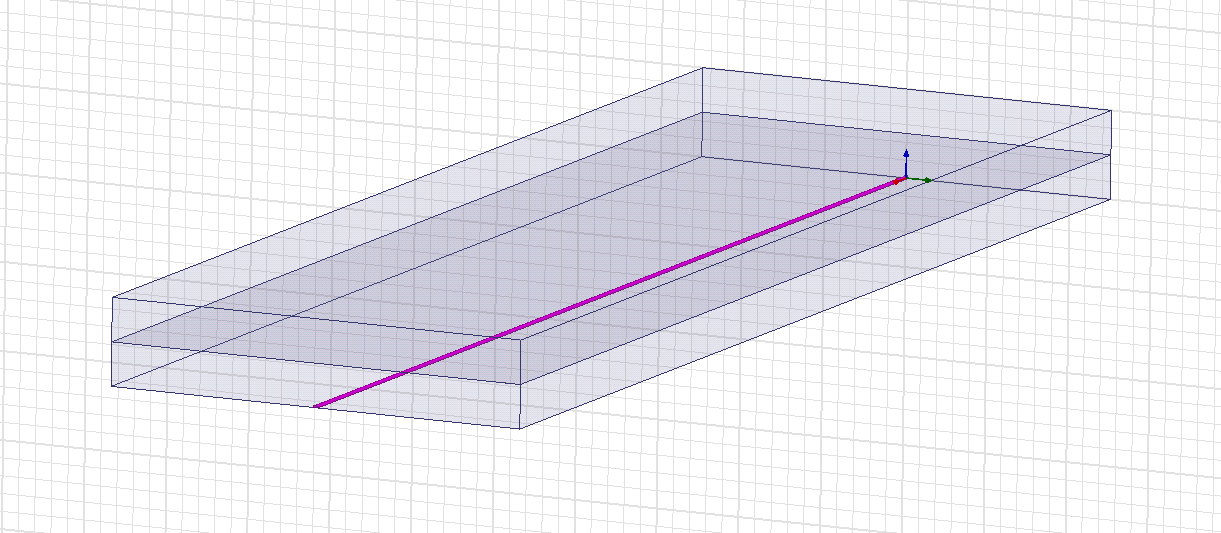
\includegraphics[width=0.5\textwidth]{Bench_Top_Measurements/figures/cross-section-coaxial-wire-measurements.png}
\end{center}
\caption{An example of the simulation model used for coaxial wire simulations. In this case a displaced single wire between two parallel plates. The wire is highlighted in purple.}
\label{fig:wire-sim-model}
\end{figure}

\subsubsection{Two Parallel Ferrite Plates}

For the simulations of two parallel ferrite plates the following parameters were used in HFSS; for the displaced single wire measurements a wire of 0.3mm in radius, and the following displacement used to acquire the total transverse terms:

\begin{enumerate}
\item{In the horizontal axis -  displaced between -6mm to +6mm at intervals of 2mm}
\item{In the vertical axis - displaced between -4mm to +4mm at intervals of 2mm.}
\end{enumerate}

For the two wire simulations, two wires of radius 0.3mm are used, with a seperation of 4mm in the x-dimension, and 3mm in the y-dimension. 4 simulation configurations are used described below:

\begin{enumerate}
\item{an adaptive mesh generation set to a convergence criterion of $S_{21}$ diverging by less than 0.005 between two subsequent solutions, at an adaptive frequency of 20MHz solving to a second order basis. A discrete frequency sweep is then carried out in the range 1-10MHz at 1MHz intervals.}
\item{an adaptive mesh generation set to a convergence criterion of $S_{21}$ diverging by less than 0.005 between two subsequent solutions, at an adaptive frequency of 200MHz solving to a second order basis. A discrete frequency sweep is then carried out in the range 10-100MHz at 10MHz intervals.}
\item{an adaptive mesh generation set to a convergence criterion of $S_{21}$ diverging by less than 0.005 between two subsequent solutions, at an adaptive frequency of 2GHz solving to a second order basis. A discrete frequency sweep is then carried out in the range 100MHz-1GHz at 100MHz intervals.}
\item{an adaptive mesh generation set to a convergence criterion of $S_{21}$ diverging by less than 0.005 between two subsequent solutions, at an adaptive frequency of 10GHz solving to a second order basis. A discrete frequency sweep is then carried out in the range 1-10GHz at 1GHz intervals.}
\end{enumerate}

These parameters are used to benefit from an appropriate mesh count for the given frequency range, thus increasing simulation speed by not using a high density mesh at frequencies where no benefits would be gained.

\begin{figure}
\subfigure[]{
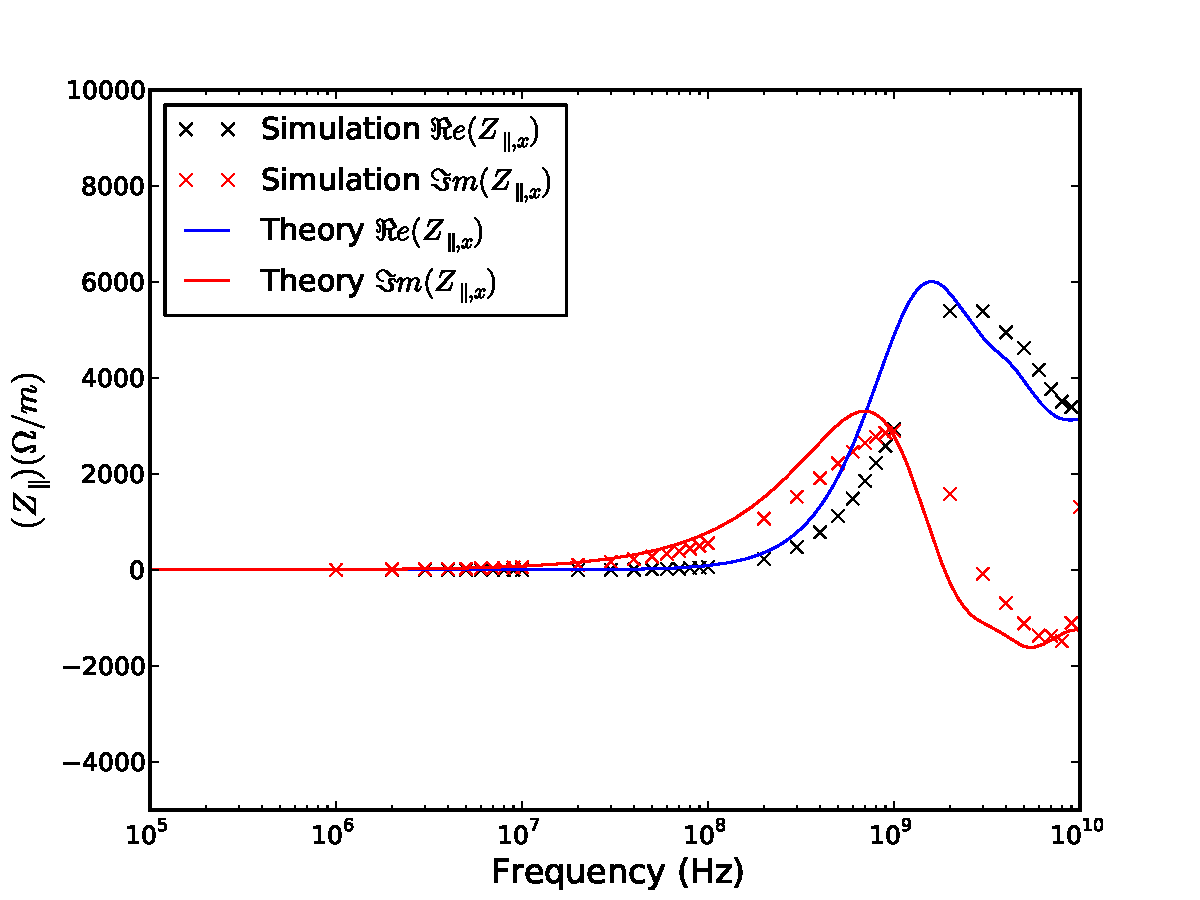
\includegraphics[width=0.5\textwidth]{Bench_Top_Measurements/figures/wire_meas/ferrite_plates/longitudinal-horizontal.pdf}
\label{fig:ferrite-plates-long-horz}
}
\subfigure[]{
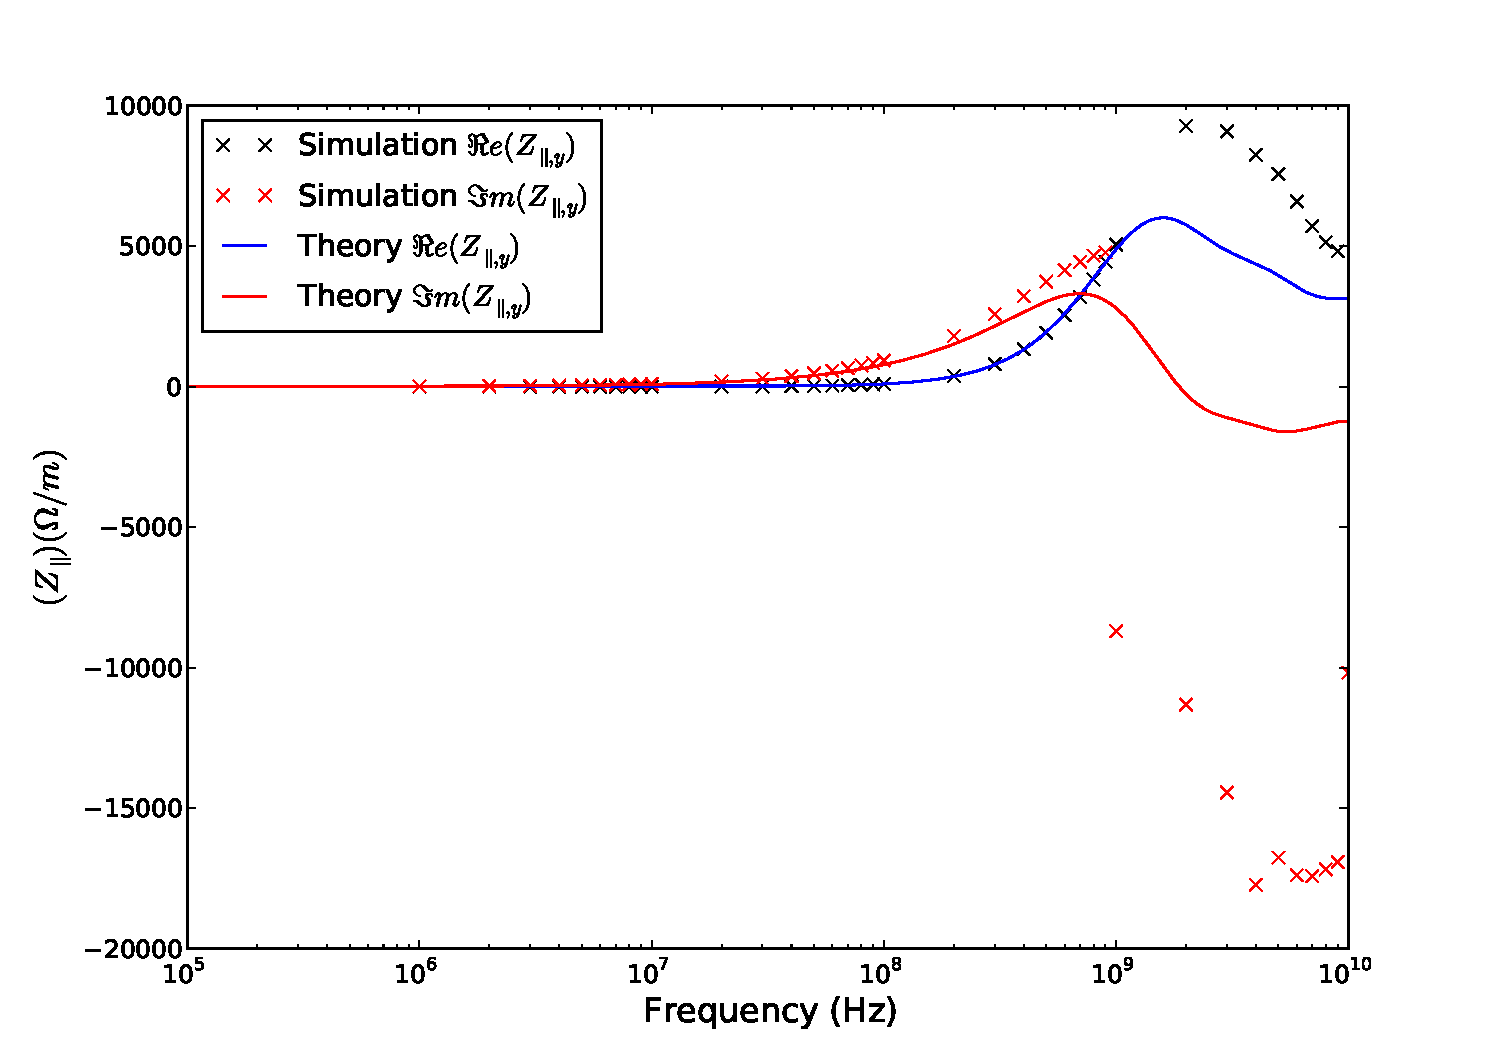
\includegraphics[width=0.5\textwidth]{Bench_Top_Measurements/figures/wire_meas/ferrite_plates/longitudinal-vertical.pdf}
\label{fig:ferrite-plates-long-vert}
}
\caption{The longitudinal impedance of two parallel ferrite plates simulated using a longitudinal coaxial wire. Presented is the impedance as measured in the horizontal plane (\subref{fig:ferrite-plates-long-horz}) and in the vertical plane \subref{fig:ferrite-plates-long-vert}.}
\label{fig:ferrite-plates-long}
\end{figure}

\begin{figure}
\subfigure[]{
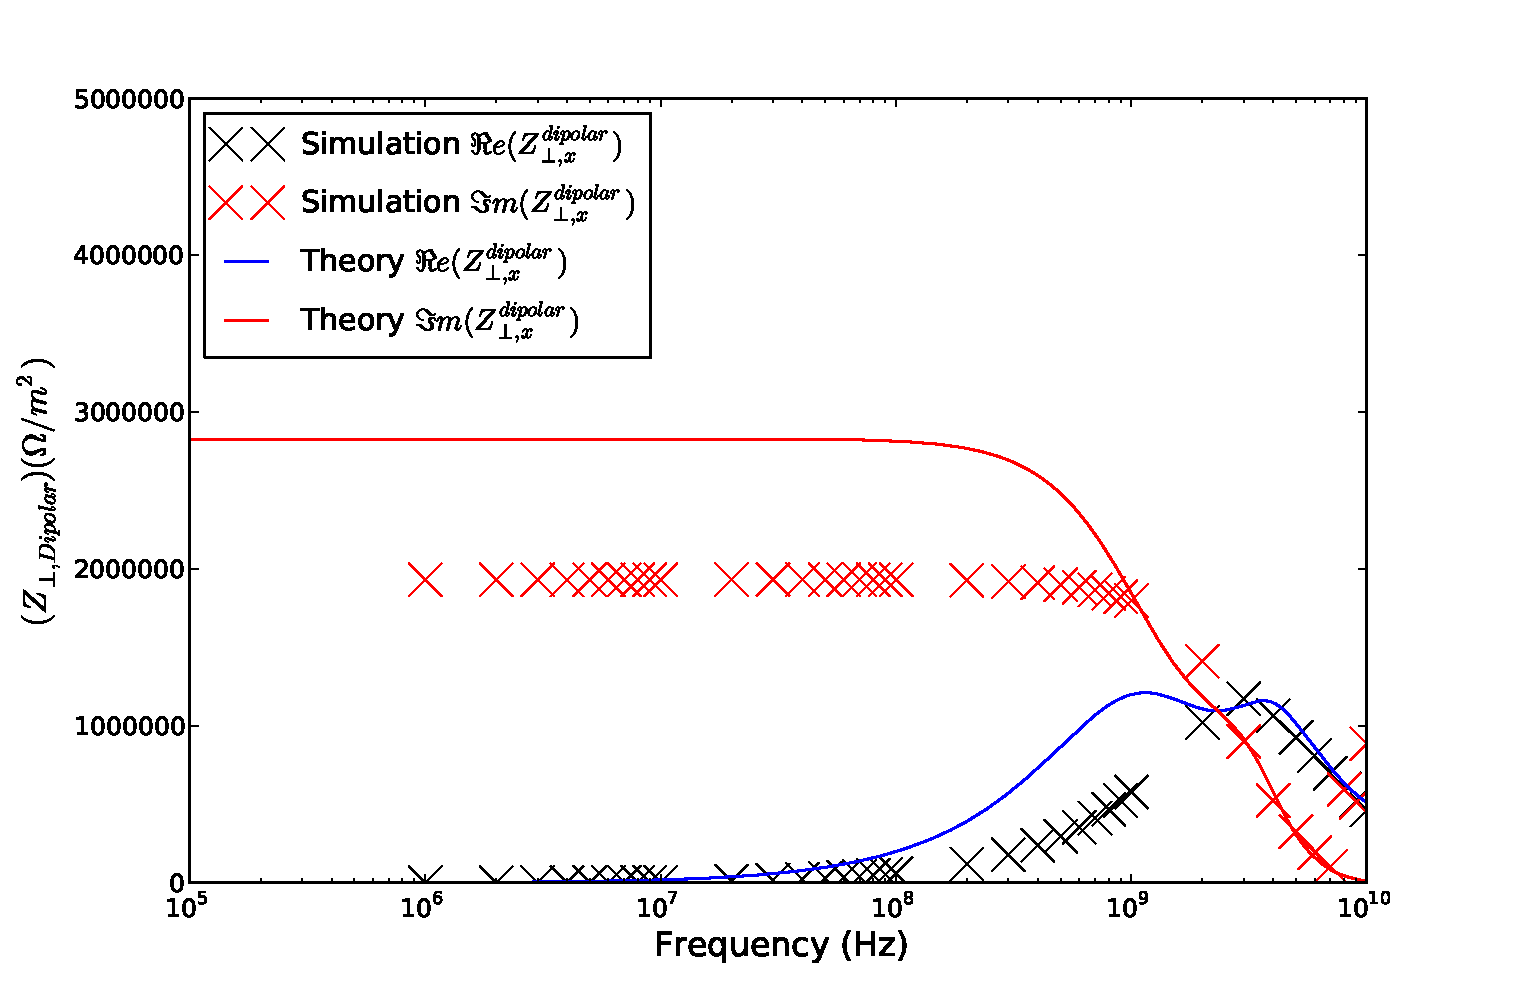
\includegraphics[width=0.5\textwidth]{Bench_Top_Measurements/figures/wire_meas/ferrite_plates/dipolar-horizontal.pdf}
\label{fig:ferrite-plates-dip-horz}
}
\subfigure[]{
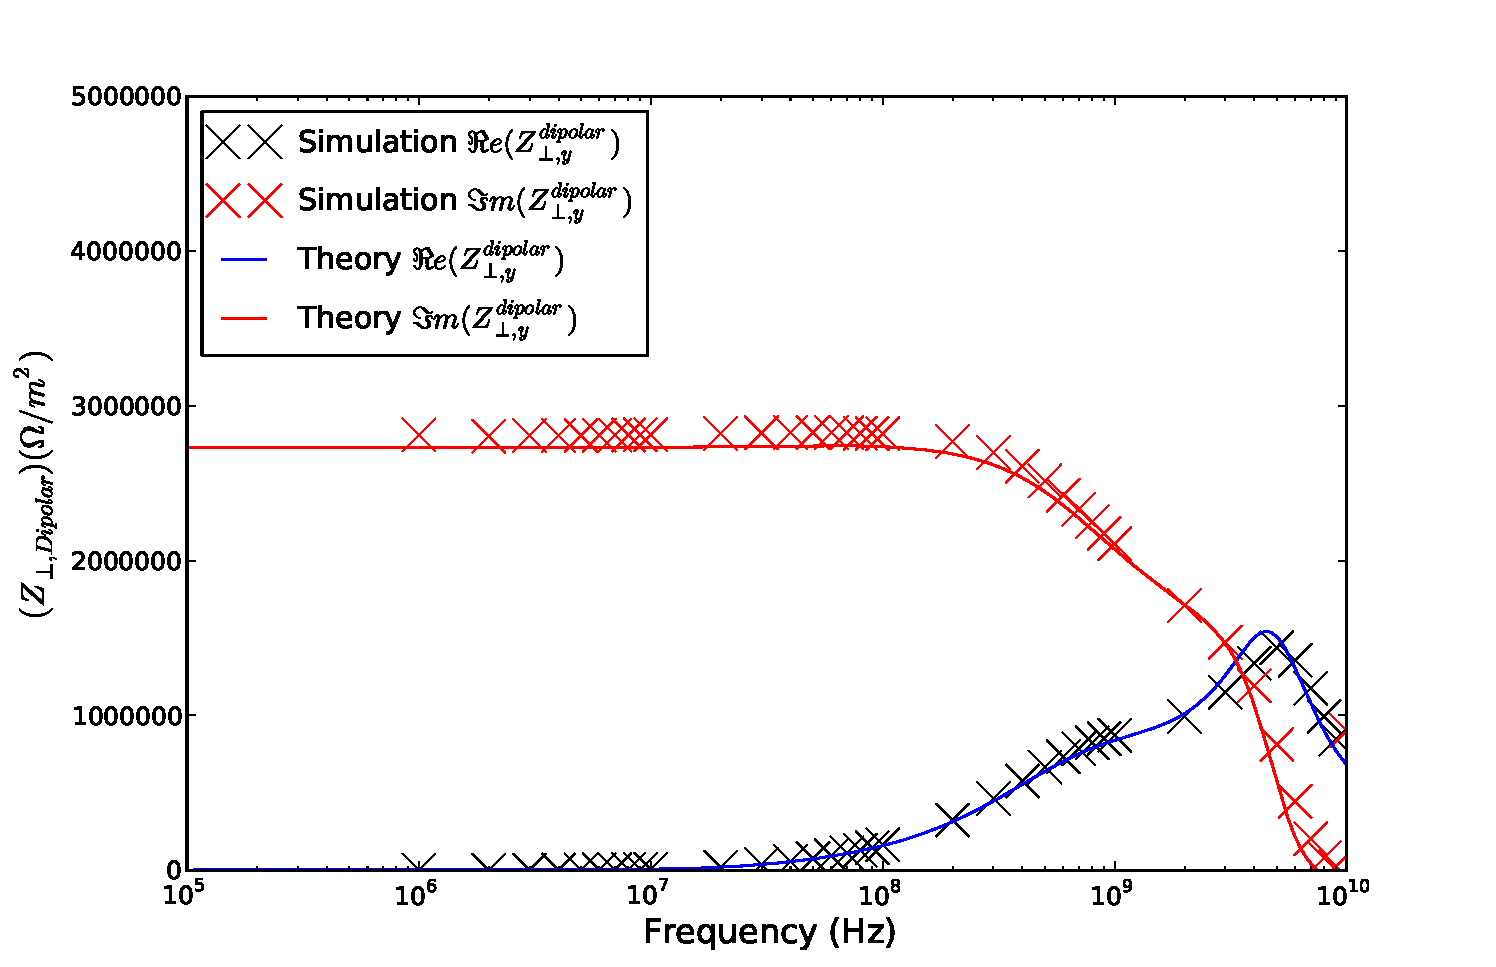
\includegraphics[width=0.5\textwidth]{Bench_Top_Measurements/figures/wire_meas/ferrite_plates/dipolar-vertical.pdf}
\label{fig:ferrite-plates-dip-vert}
}
\caption{The dipolar impedance of two parallel ferrite plates simulated using two longitudinal coaxial wires. Presented are the impedances as measured in the horizontal plane (\subref{fig:ferrite-plates-dip-horz}) and in the vertical plane \subref{fig:ferrite-plates-dip-vert}.}
\label{fig:ferrite-plates-dipolar}
\end{figure}

\begin{figure}
\subfigure[]{
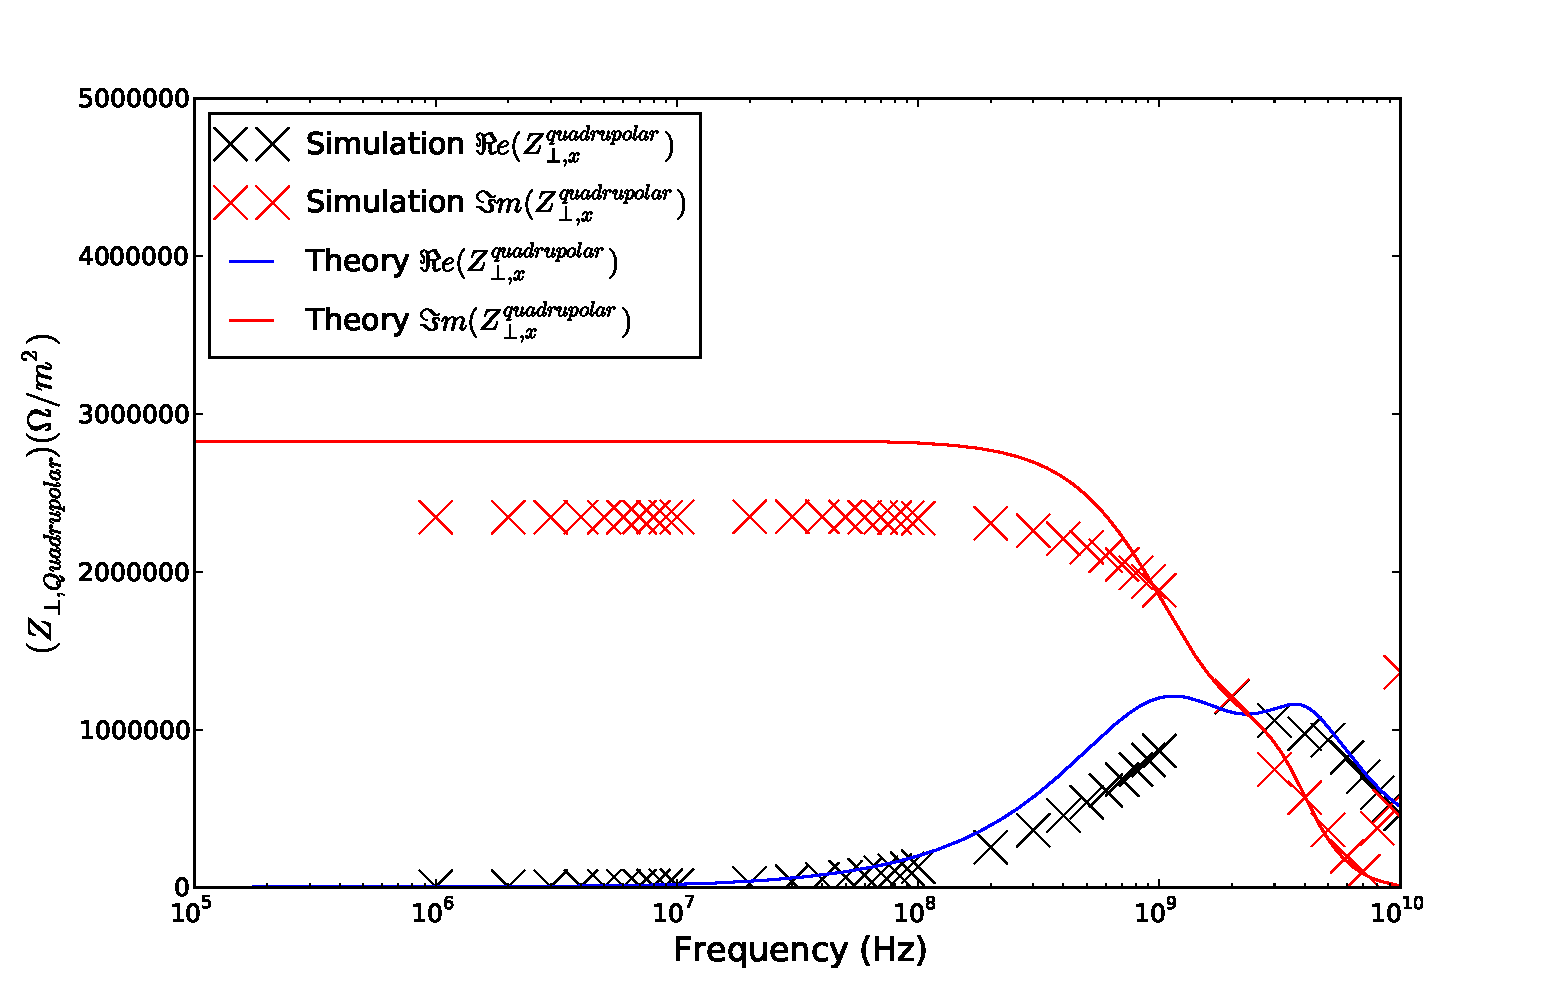
\includegraphics[width=0.5\textwidth]{Bench_Top_Measurements/figures/wire_meas/ferrite_plates/quadrupolar-horizontal.pdf}
\label{fig:ferrite-plates-quad-horz}
}
\subfigure[]{
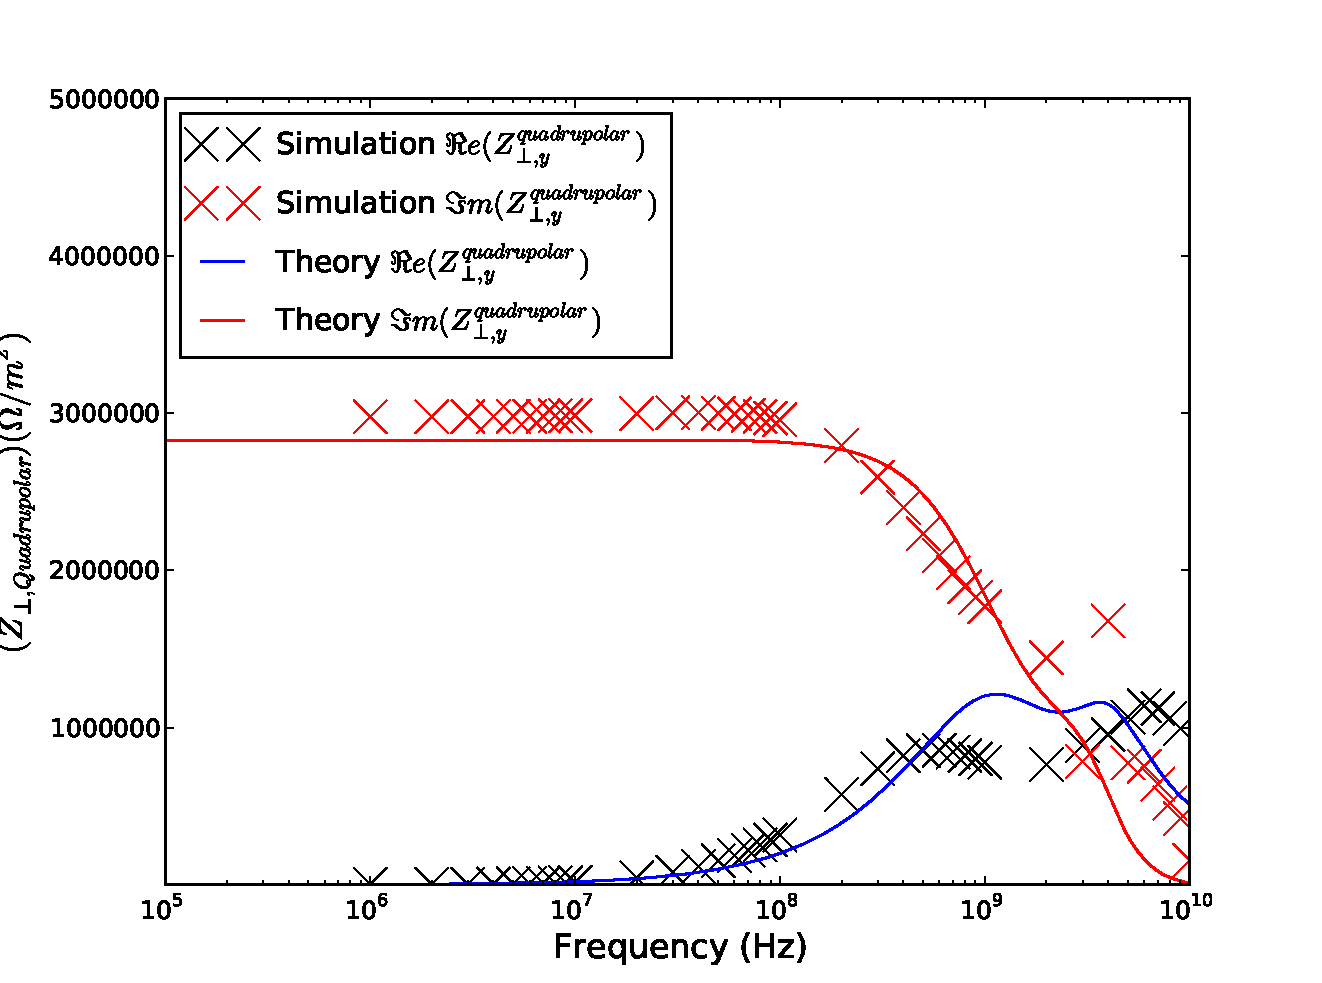
\includegraphics[width=0.5\textwidth]{Bench_Top_Measurements/figures/wire_meas/ferrite_plates/quadrupolar-vertical.pdf}
\label{fig:ferrite-plates-quad-vert}
}
\caption{The quadrupolar impedance of two parallel ferrite plates simulated using a combination of displaced single wire simulated measurements and two wire simulated measurements. Presented is the impedance as measured in the horizontal plane (\subref{fig:ferrite-plates-quad-horz}) and in the vertical plane \subref{fig:ferrite-plates-quad-vert}.}
\label{fig:ferrite-plates-quadrupolar}
\end{figure}

The longitudinal impedance is determined by taking the constant term for a series of simulated displaced wire measurements in both the vertical and horizontal planes is shown in Fig.~\ref{fig:ferrite-plates-long}. It can be seen that in the frequency range below 100MHz the agreement between the coaxial wire results and the analytical results is very good in both the vertical and horizontal plane. Above 100MHz the agreement for the real components is very good for both results, however the imaginary component in the vertical plane displays some substantial disagreement. This is likely due to the high mesh density required to correctly evaluate the phase change along the length of the simulated structure. A higher mesh density may correct this, however limits of computational resource presently make this unfeasible.

The agreement between the simulations of the vertical dipolar impedance and the theoretical model is excellent across all frequencies for both the real and imaginary components. The agreement below 100MHz and above 1GHz is very good for the horizontal dipolar, with some divergence in the constant term of the imaginary impedance. The key difference is the failure of the coaxial method to resolve one of the peaks in the real impedance. The results for the dipolar impedance are shown in Fig.~\ref{fig:ferrite-plates-dipolar}.

The results for the quadrupolar impedance are shown in Fig.~\ref{fig:ferrite-plates-quadrupolar}. The vertical simulations agree well with the theory, correctly identifying the two peaks in the quadrupolar impedance. The agreement for the horizontal simulations with theory is less good. This can be explained by the derivation of the horizontal quadrupolar being highly dependent on the quality of the horizontal dipolar impedance results due to them cancelling each other to form the total transverse impedance. As the horizontal dipolar impedance does not resolve the subpeaks neither does the horizontal quadrupolar impedance calculations.

\subsubsection{Two Parallel Graphite Plates}

For the simulations of measurements of two parallel graphite plates, two different methods were used. Due to the non-ferritic properties of the graphite, it is possible to use Maxwell3D to simulate the power loss at lower frequencies, thus acquiring the real component of the impedance for low frequencies, in addition to using the classical coaxial wire method at higher frequencies in HFSS.

For the simulations of the power loss in Maxwell3D the following parameters were used; for the displaced single wire measurements a wire of 0.5mm radius is modelled, and the following displacement used to acquire the total transverse terms:

\begin{enumerate}
\item{In the horizontal axis -  displaced between -6mm to +6mm at intervals of 2mm}
\item{In the vertical axis - displaced between -4mm to +4mm at intervals of 2mm.}
\end{enumerate}

For the two wire simulations, two wires of radius 0.3mm are modelled, with a seperation of 8mm in the x-dimension, and 4mm in the y-dimension. Five simulation configurations are used as described below:

\begin{enumerate}
\item{an adaptive mesh generation set to a convergence criterion of $S_{21}$ diverging by less than 0.005 between two subsequent solutions, at an adaptive frequency of 20kHz solving to a second order basis. A discrete frequency sweep is then carried out in the range 1-10kHz at 1kHz intervals.}
\item{an adaptive mesh generation set to a convergence criterion of $S_{21}$ diverging by less than 0.005 between two subsequent solutions, at an adaptive frequency of 200kHz solving to a second order basis. A discrete frequency sweep is then carried out in the range 10-100kHz at 10kHz intervals.}
\item{an adaptive mesh generation set to a convergence criterion of $S_{21}$ diverging by less than 0.005 between two subsequent solutions, at an adaptive frequency of 2MHz solving to a second order basis. A discrete frequency sweep is then carried out in the range 100kHz-1MHz at 100kHz intervals.}
\item{an adaptive mesh generation set to a convergence criterion of $S_{21}$ diverging by less than 0.005 between two subsequent solutions, at an adaptive frequency of 10MHz solving to a second order basis. A discrete frequency sweep is then carried out in the range 1-10MHz at 1MHz intervals.}
\item{an adaptive mesh generation set to a convergence criterion of $S_{21}$ diverging by less than 0.005 between two subsequent solutions, at an adaptive frequency of 100MHz solving to a second order basis. A discrete frequency sweep is then carried out in the range 10-100MHz at 10MHz intervals.}
\end{enumerate}

These parameters are used to benefit from an appropriate mesh count for the given frequency range, thus increasing simulation speed by not using a high density mesh at frequencies where no benefits would be gained.

For the simulations of the single displaced wire in HFSS the following parameters were used; for the displaced single wire measurements a wire of 0.3mm in radius is modelled, and the following displacements to acquire the total transverse terms:

\begin{enumerate}
\item{In the horizontal axis -  displaced between -6mm to +6mm at intervals of 2mm}
\item{In the vertical axis - displaced between -4mm to +4mm at intervals of 2mm.}
\end{enumerate}

For the two wire simulations, two wires of radius 0.3mm are modelled, with a seperation of 4mm in the x-dimension, and 3mm in the y-dimension. Three simulations configuration are used as described below:

\begin{enumerate}
\item{an adaptive mesh generation set to a convergence criterion of $S_{21}$ diverging by less than 0.005 between two subsequent solutions, at an adaptive frequency of 20MHz solving to a second order basis. A discrete frequency sweep is then carried out in the range 1-10MHz at 1MHz intervals.}
\item{an adaptive mesh generation set to a convergence criterion of $S_{21}$ diverging by less than 0.005 between two subsequent solutions, at an adaptive frequency of 200MHz solving to a second order basis. A discrete frequency sweep is then carried out in the range 10-100MHz at 10MHz intervals.}
\item{an adaptive mesh generation set to a convergence criterion of $S_{21}$ diverging by less than 0.005 between two subsequent solutions, at an adaptive frequency of 2GHz solving to a second order basis. A discrete frequency sweep is then carried out in the range 100MHz-1GHz at 100MHz intervals.}
\end{enumerate}

As before these parameters are used to benefit from an appropriate mesh count for the given frequency range, thus increasing simulation speed by not using a high density mesh at frequencies where no benefits would be gained.

\begin{figure}
\subfigure[]{
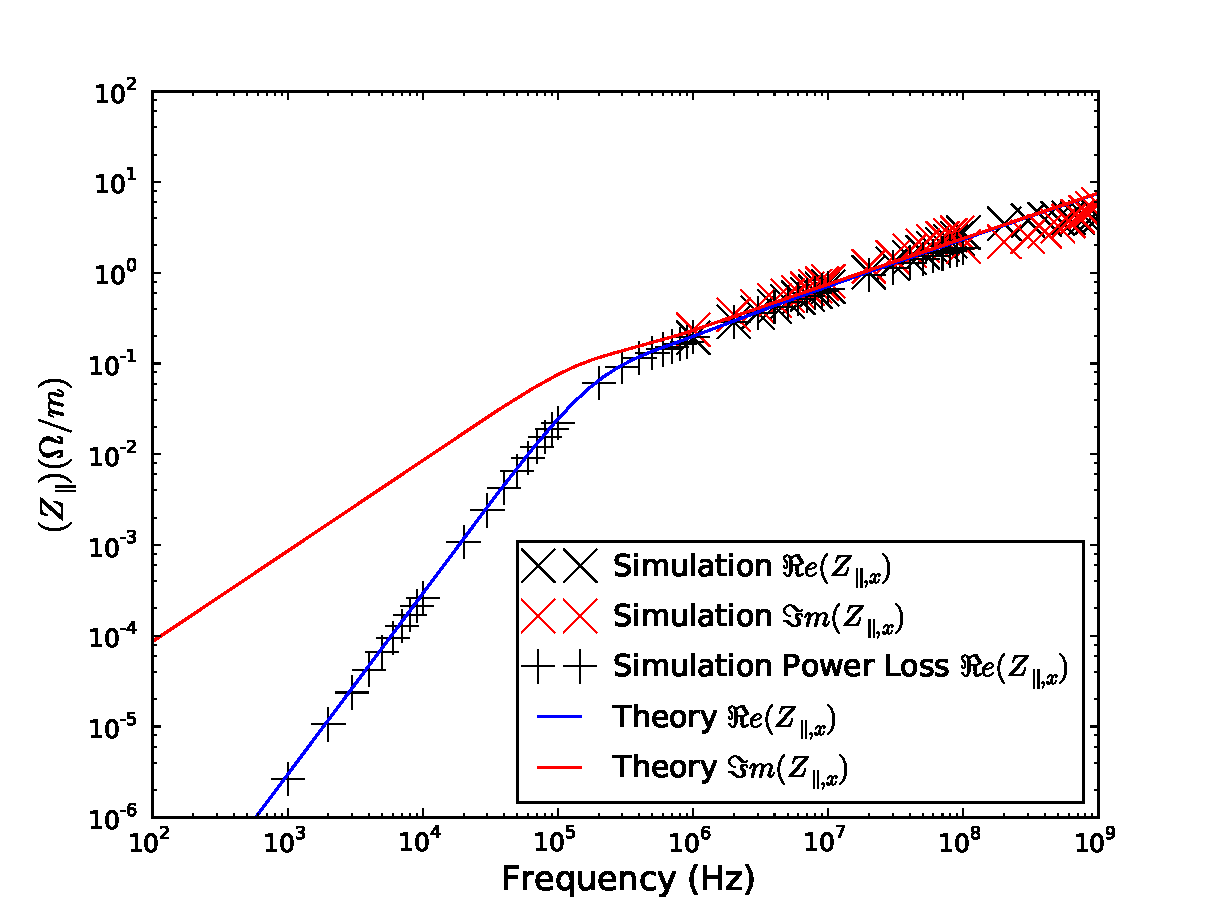
\includegraphics[width=0.5\textwidth]{Bench_Top_Measurements/figures/wire_meas/graphite_plates/longitudinal-horizontal.pdf}
\label{fig:graph-plates-long-horz}
}
\subfigure[]{
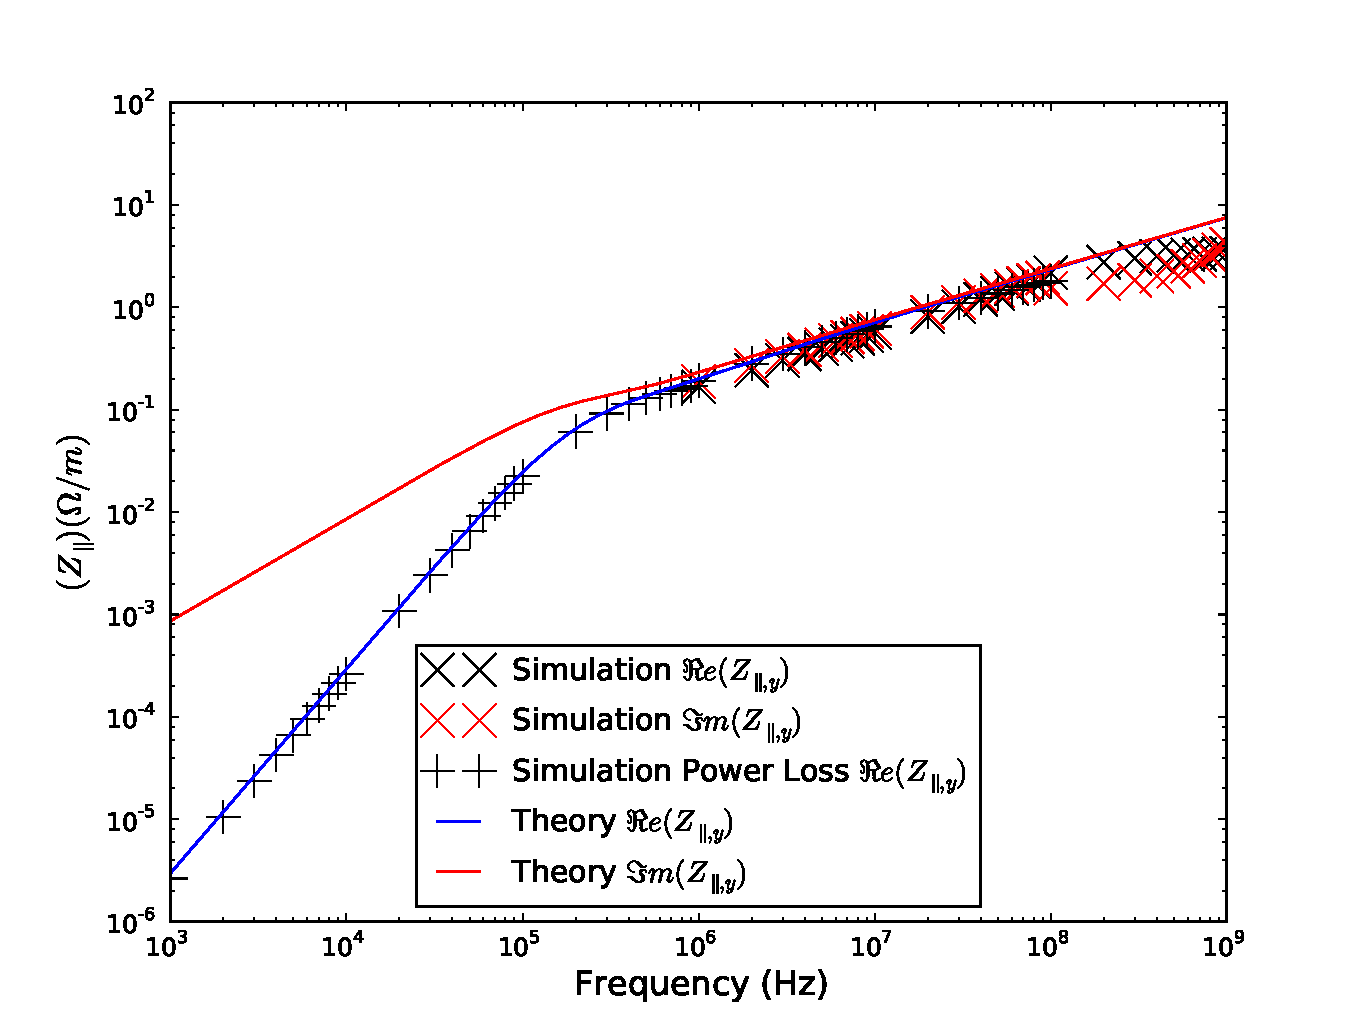
\includegraphics[width=0.5\textwidth]{Bench_Top_Measurements/figures/wire_meas/graphite_plates/longitudinal-vertical.pdf}
\label{fig:graph-plates-long-vert}
}
\caption{The longitudinal impedance of two parallel graphite plates as measured by taking the constant term of a quadratic equation fitted to a series of displaced single wire simulated measurements. Shown are simulated measurements acquired from fitting displacements in \subref{fig:graph-plates-long-horz} horizontal axis and in \subref{fig:graph-plates-long-vert} the vertical axis.}
\label{fig:graph-plates-long-imp}
\end{figure}

\begin{figure}
\subfigure[]{
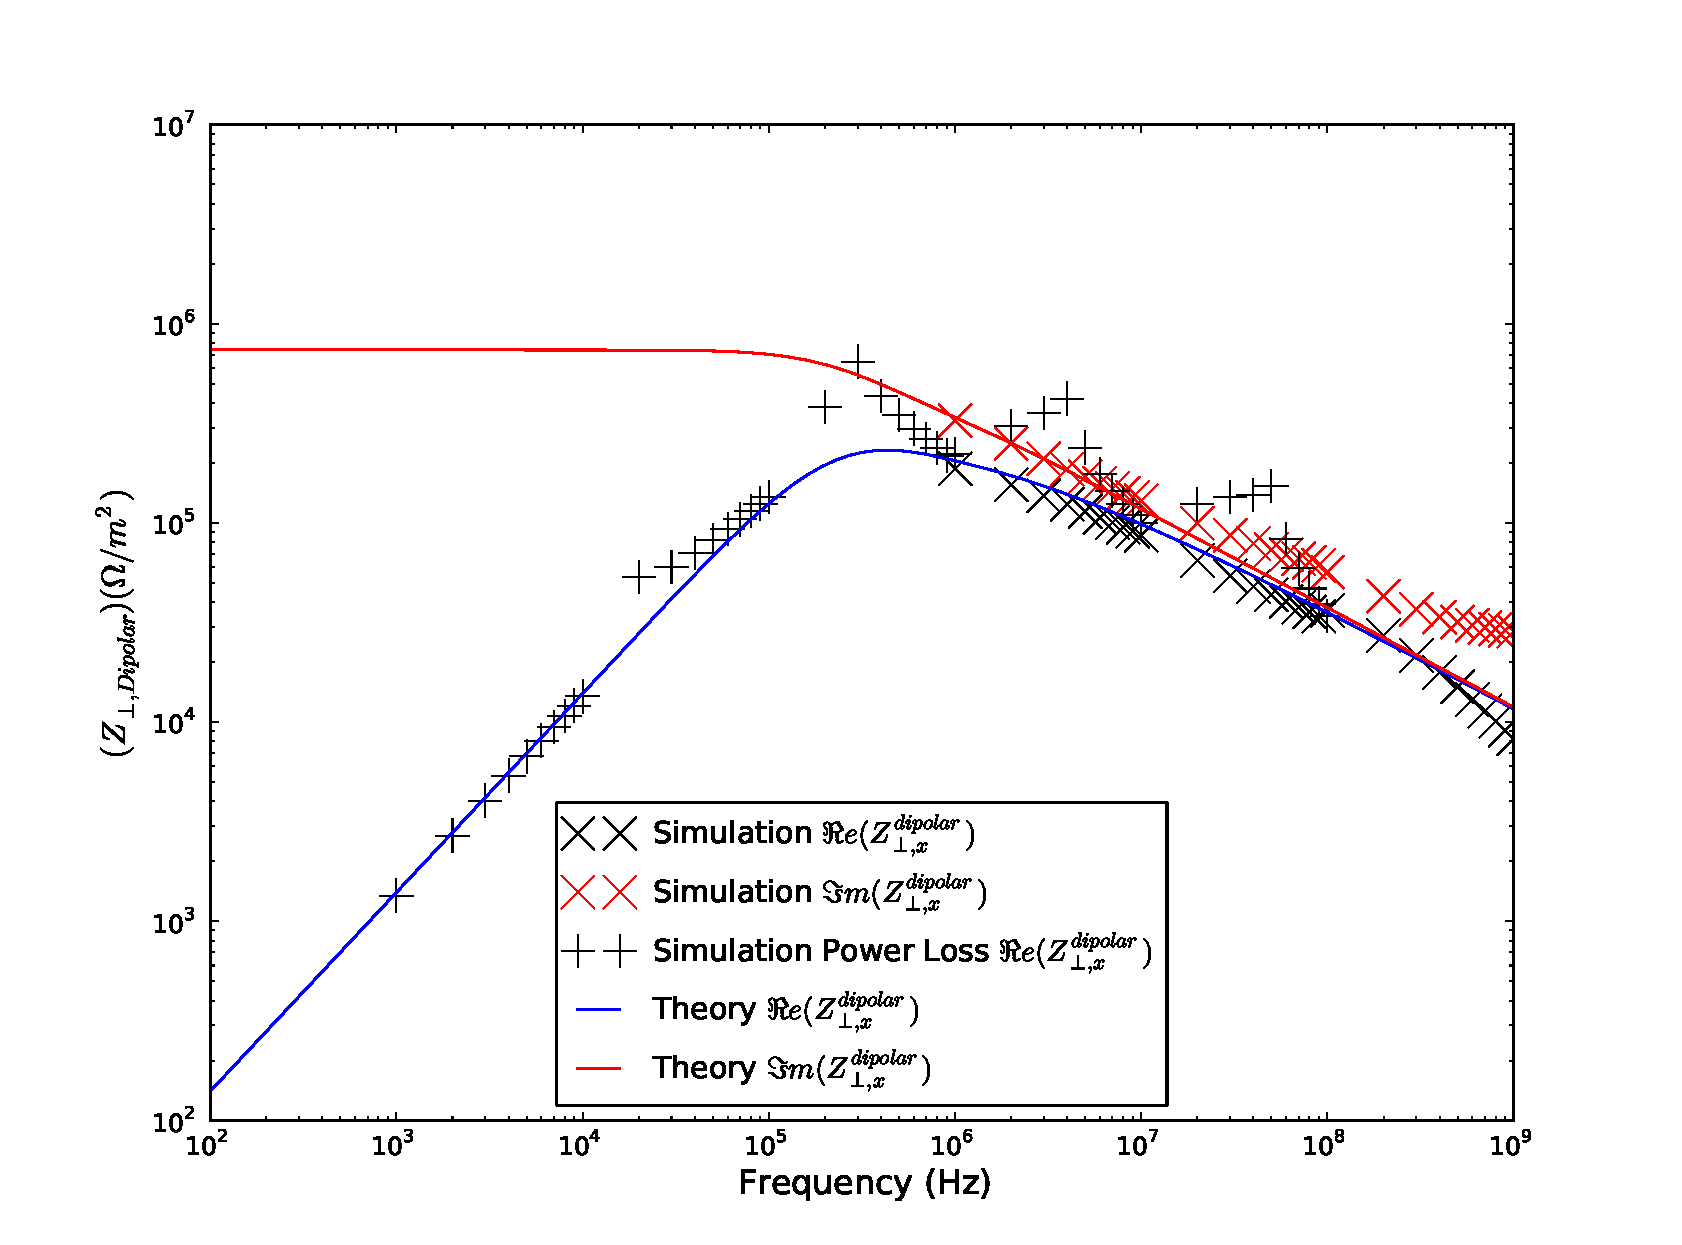
\includegraphics[width=0.5\textwidth]{Bench_Top_Measurements/figures/wire_meas/graphite_plates/dipolar-horizontal.pdf}
\label{fig:graph-plates-dip-horz}
}
\subfigure[]{
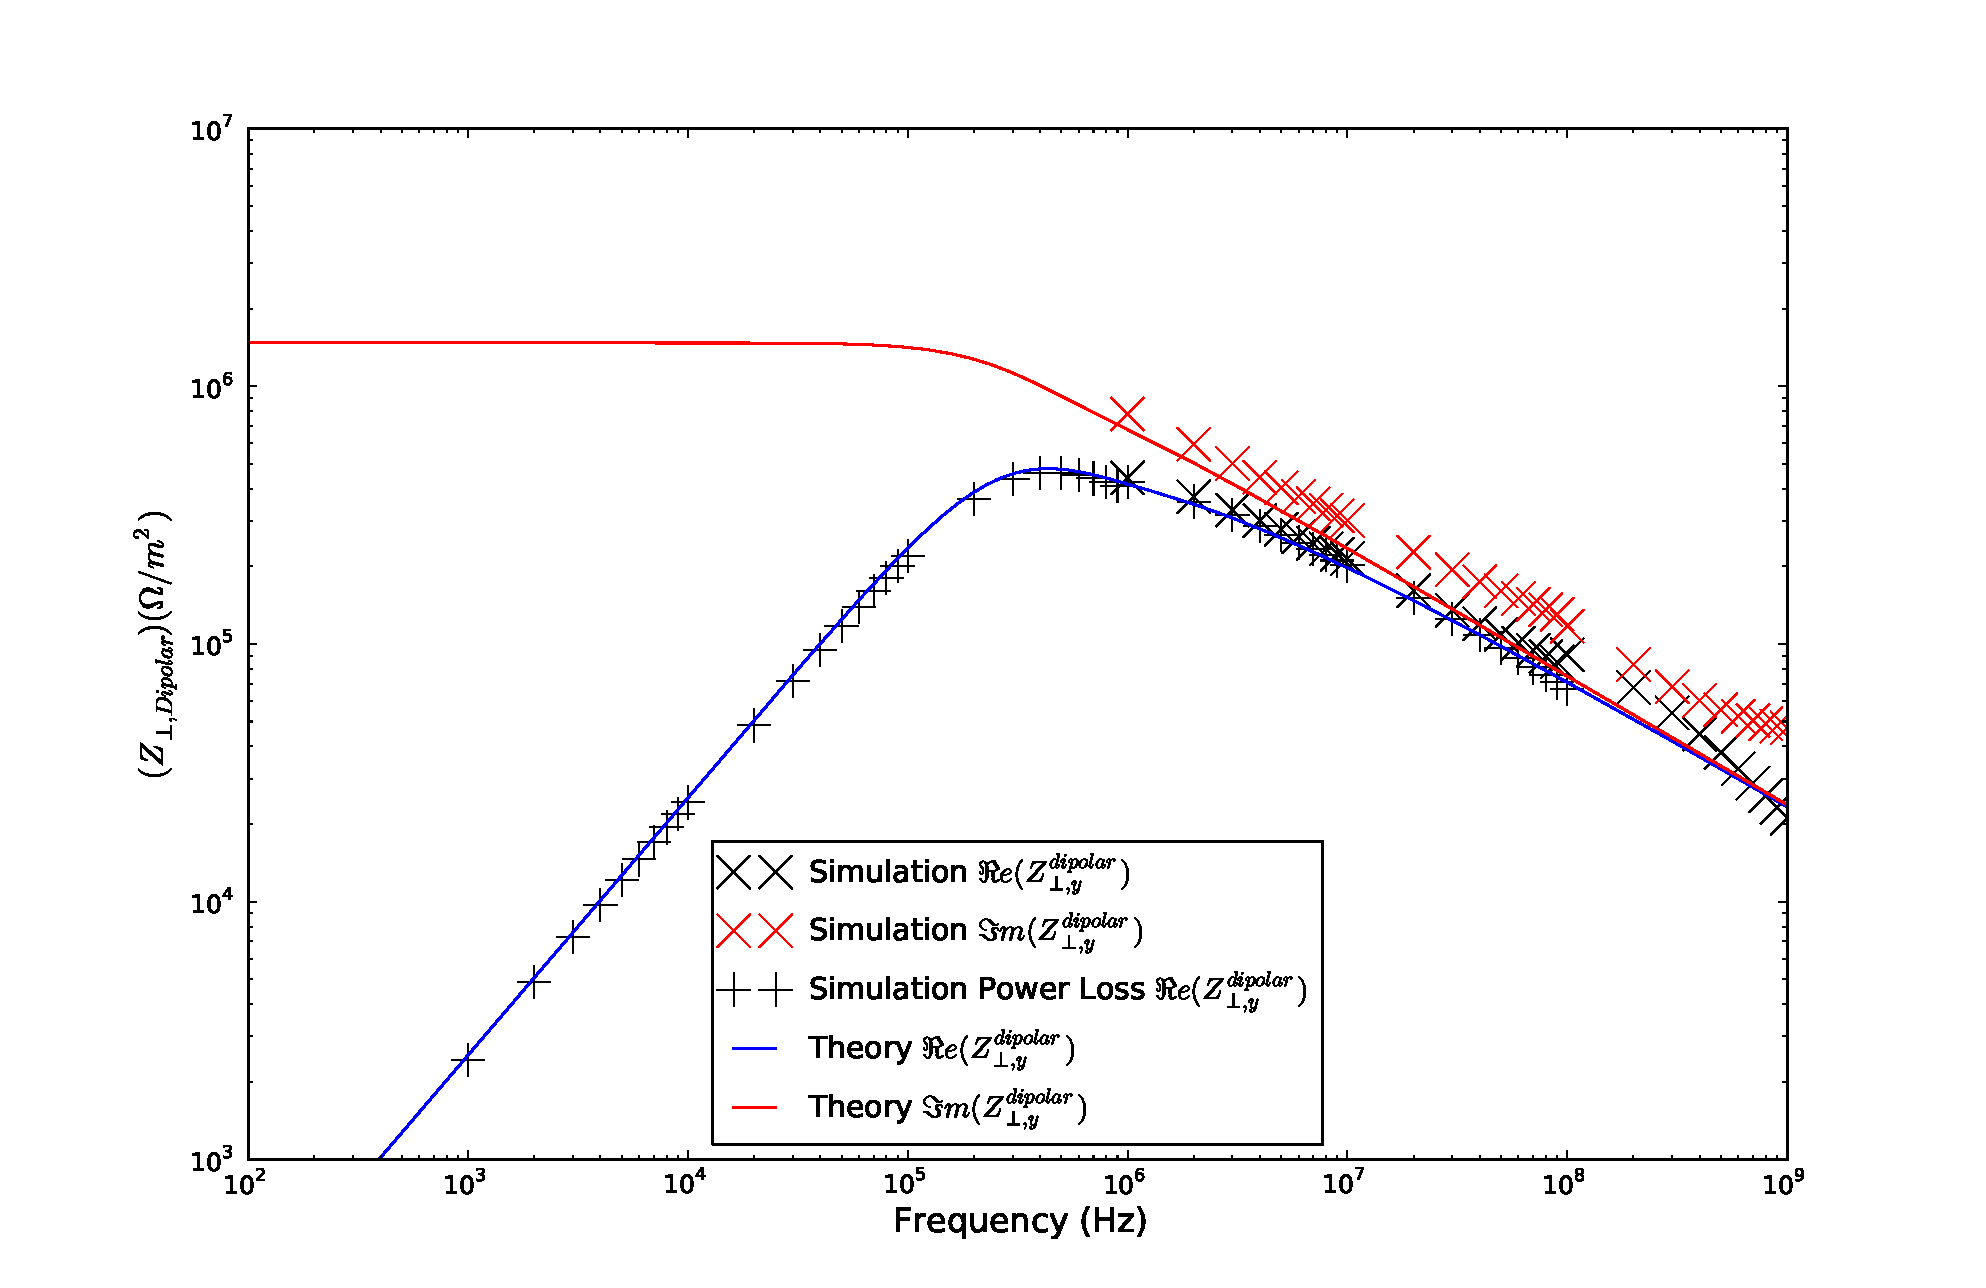
\includegraphics[width=0.5\textwidth]{Bench_Top_Measurements/figures/wire_meas/graphite_plates/dipolar-vertical.pdf}
\label{fig:graph-plates-dip-vert}
}
\caption{The dipolar impedance of two parallel graphite plates measured using two longitudinal coaxial wires. Presented is the impedance as measured in the horizontal plane (\subref{fig:graph-plates-dip-horz}) and in the vertical plane \subref{fig:graph-plates-dip-vert}.}
\label{fig:graph-plates-dipolar}
\end{figure}

\begin{figure}
\begin{center}
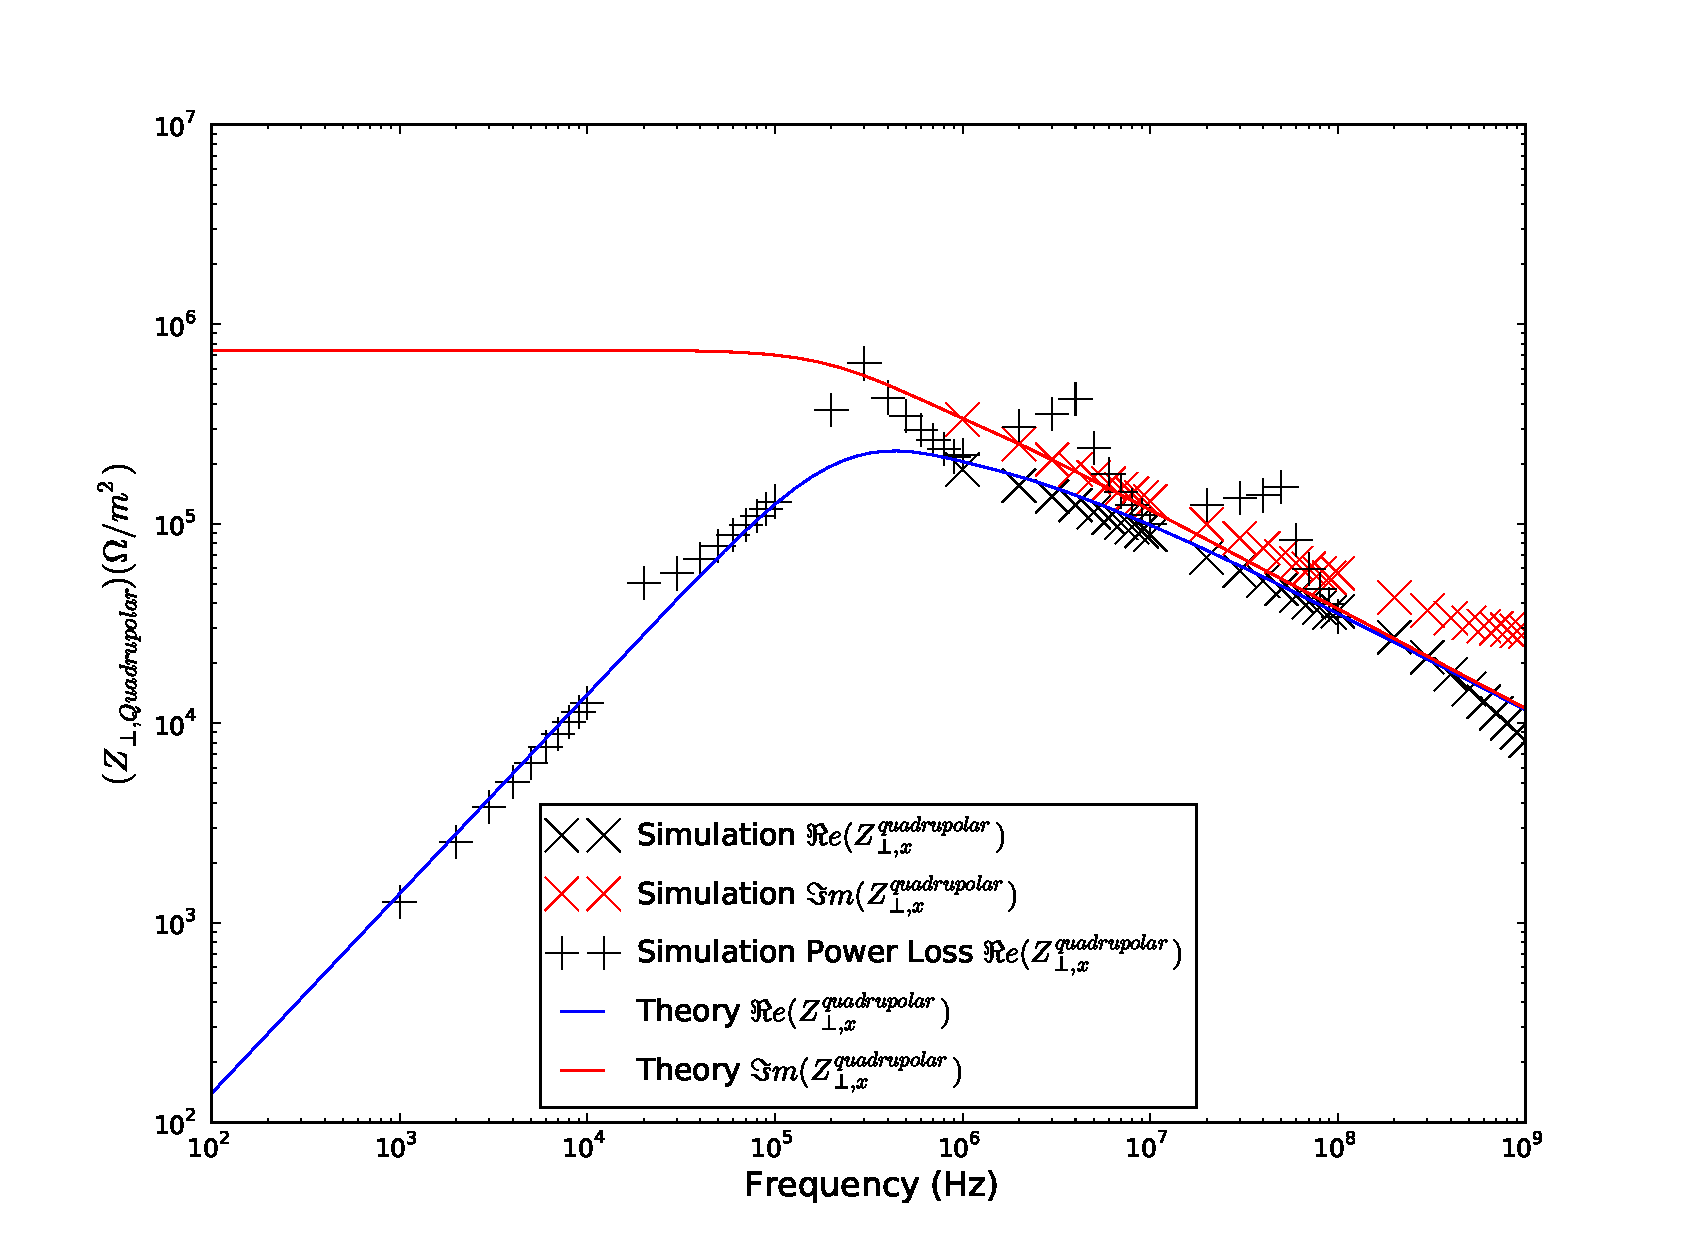
\includegraphics[width=0.75\textwidth]{Bench_Top_Measurements/figures/wire_meas/graphite_plates/quadrupolar-horizontal.pdf}
\end{center}
\caption{The quadrupolar impedance of two parallel graphite plates measured using a combination of displaced single wire measurements and two wire mesurements.}
\label{fig:graph-plates-quadrupolar}
\end{figure}

The longitudinal impedance in Fig.~\ref{fig:graph-plates-long-imp}. It can be seen that the agreement for both the real component is excellent across the entire frequency range, for simulations using both the classical coaxial wire method and the power loss method of Maxwell3D. The agreement is also good for the imaginary component over much of the frequency range, becoming worse above 100MHz. This is likely due to insufficient mesh density to catch the relatively small phase shift at this frequency range.

The agreement between simulations and theory for the vertical dipolar impedance can be seen to be very good over the entire frequency range also (see Fig.~\ref{fig:graph-plates-dip-vert}). The results at low frequencies (below 100kHz) for the power loss method and at all frequencies for the classical coaxial wire method for the horizontal dipolar impedance agree very well with theory (see Fig.~\ref{fig:graph-plates-dip-horz}). The quadrupolar impedance is shown in Fig.~\ref{fig:graph-plates-quadrupolar}, and again the agreement between the simulated measurements and theory can be seen to be good over the entire frequency range, using both the power loss method and the classical coaxial wire method. However, the power loss method does predict peaks at the lower part of each frequency sweep that are not predicted in either tha theoretical model or the measurements with the coaxial wire method in HFSS.

\subsubsection{C-Core Ferrite Kicker}

To test the measurement method for an asymmetric structure a model of the C-core ferrite kicker magnet was used, as shown in Fig.\ref{fig:zannini-model}, the analytical details of which are given in \cite{Zannini:cCoreFerrite}. Key in this type of structure is that it predicts a non-zero constant transverse impedance term as well as the quadrupolar terms, thus we may completely evaluate the asymmetric measurement method. For these simulations a structure of $a=15$mm, $r=20$mm, $\theta = \pi / 2$, and $100$mm in length was used. Simulations were carried out using the classical coaxial wire method as simulated in HFSS.

The following parameters were used for the simulations; wire of 0.2mm in radius, and the following displacement used to acquire the total transverse terms:

\begin{enumerate}
\item{In the horizontal axis -  displaced between -5mm to +5mm at intervals of 1mm.}
\item{In the vertical axis - displaced between -5mm to +5mm at intervals of 1mm.}
\end{enumerate}

For the two wire simulations, two wires of radius 0.2mm are modelled, with a separation of 2mm in the x-dimension, and 2mm in the y-dimension. Four simulation configurations were used which are described below:

\begin{enumerate}
\item{an adaptive mesh generation set to a convergence criterion of $S_{21}$ diverging by less than 0.005 between two subsequent solutions, at an adaptive frequency of 20MHz solving to a second order basis. A discrete frequency sweep is then carried out in the range 1-10MHz at 1MHz intervals.}
\item{an adaptive mesh generation set to a convergence criterion of $S_{21}$ diverging by less than 0.005 between two subsequent solutions, at an adaptive frequency of 200MHz solving to a second order basis. A discrete frequency sweep is then carried out in the range 10-100MHz at 10MHz intervals.}
\item{an adaptive mesh generation set to a convergence criterion of $S_{21}$ diverging by less than 0.005 between two subsequent solutions, at an adaptive frequency of 2GHz solving to a second order basis. A discrete frequency sweep is then carried out in the range 100MHz-1GHz at 100MHz intervals.}
\item{an adaptive mesh generation set to a convergence criterion of $S_{21}$ diverging by less than 0.005 between two subsequent solutions, at an adaptive frequency of 10GHz solving to a second order basis. A discrete frequency sweep is then carried out in the range 1-10GHz at 1GHz intervals.}
\end{enumerate}

These parameters are used to benefit from an appropriate mesh count for the given frequency range, thus increasing simulation speed by not using a high density mesh at frequencies where no benefits would be gained.

\begin{figure}
\subfigure[]{
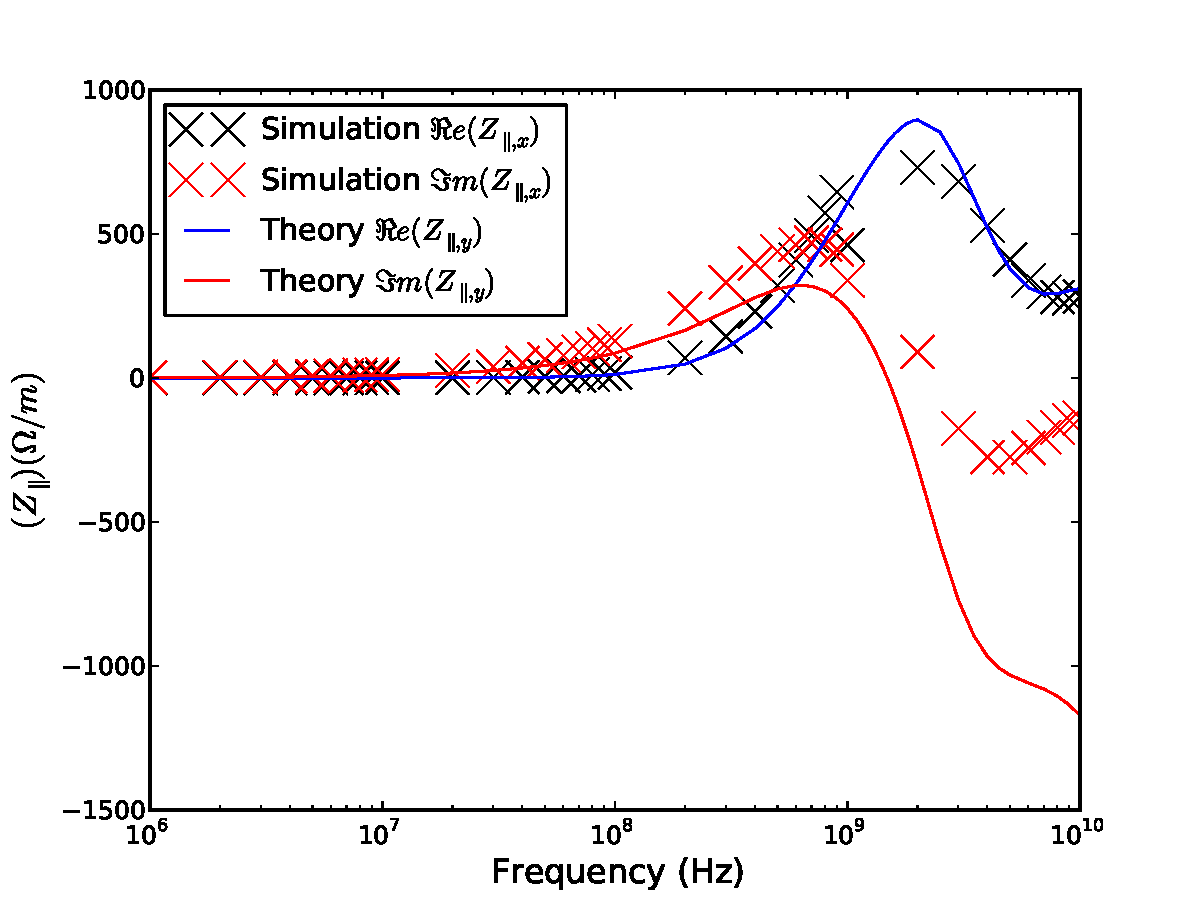
\includegraphics[height=0.35\textwidth]{Bench_Top_Measurements/figures/wire_meas/ferrite-c-core/longitudinal-impedance.pdf}
\label{fig:c-core-longitudinal}
}
\subfigure[]{
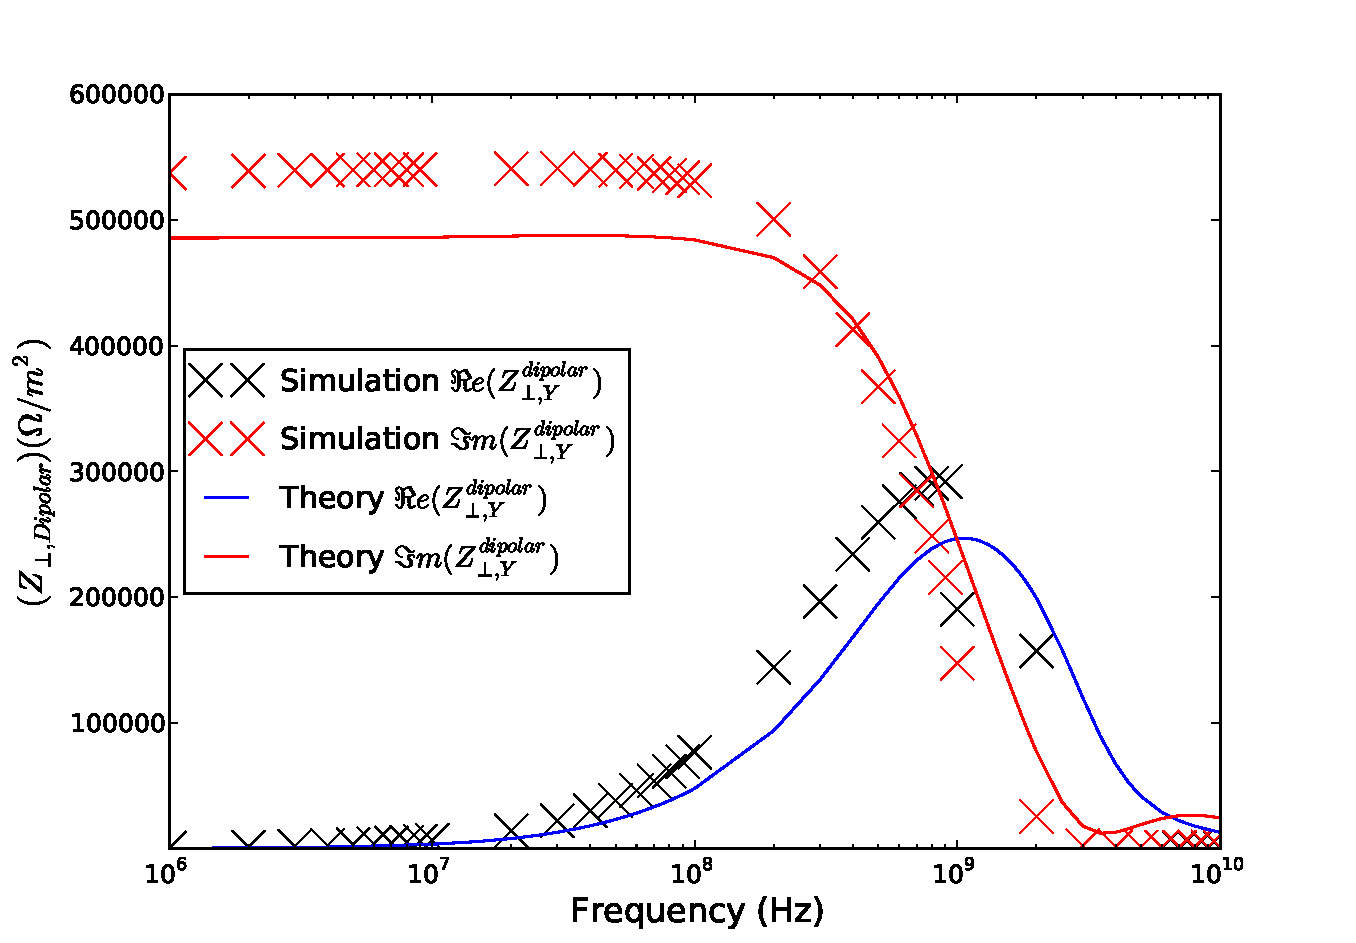
\includegraphics[height=0.35\textwidth]{Bench_Top_Measurements/figures/wire_meas/ferrite-c-core/dipolar-vertical-impedance.pdf}
\label{fig:c-core-dipolar}
}
\subfigure[]{
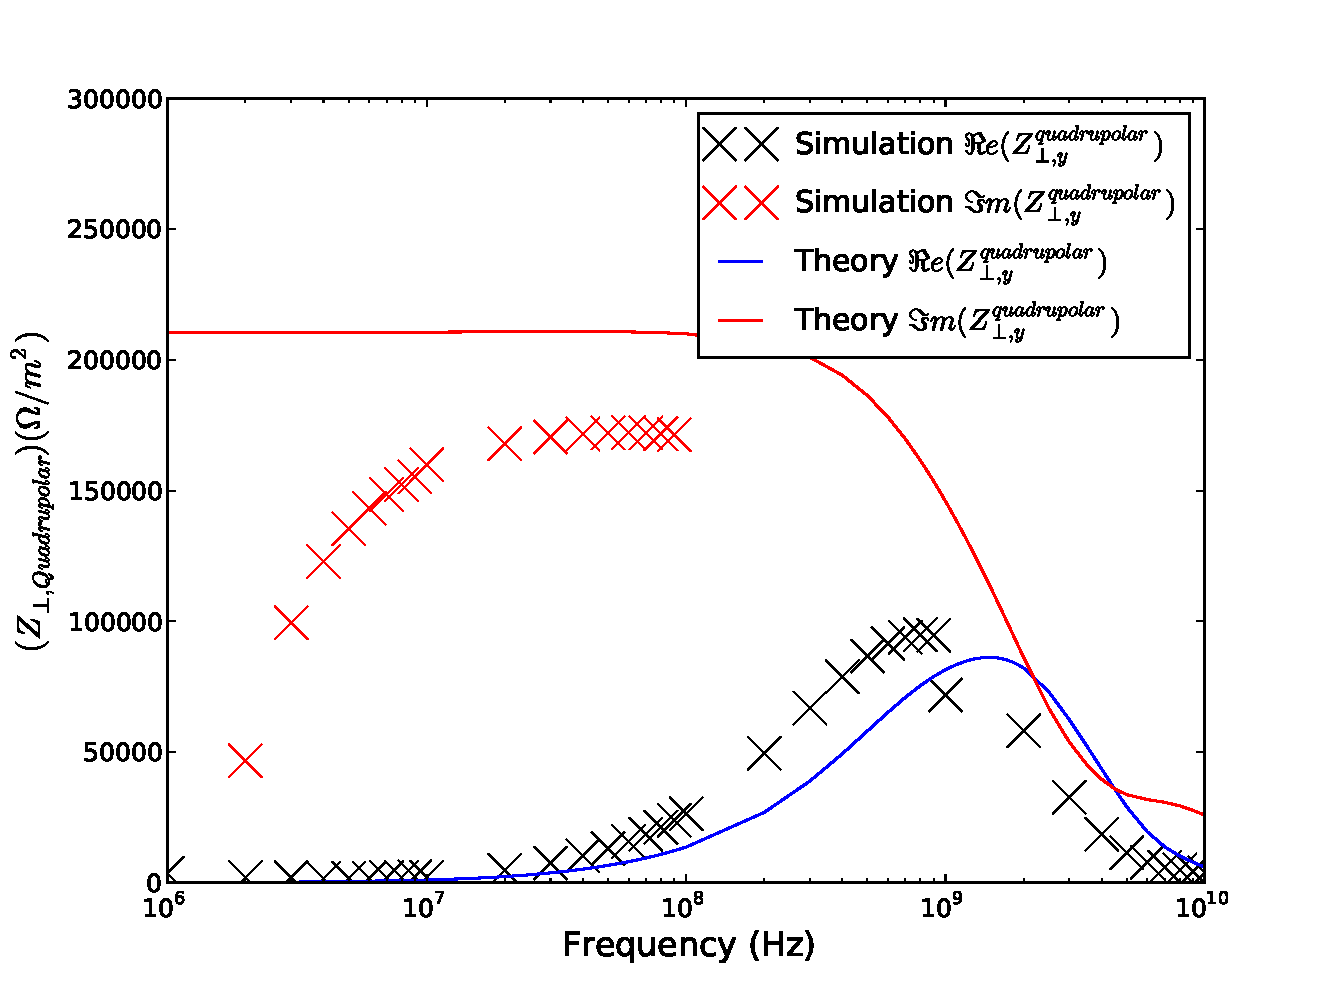
\includegraphics[height=0.35\textwidth]{Bench_Top_Measurements/figures/wire_meas/ferrite-c-core/quadrupolar-vertical-impedance.pdf}
\label{fig:c-core-quadrupolar}
}
\subfigure[]{
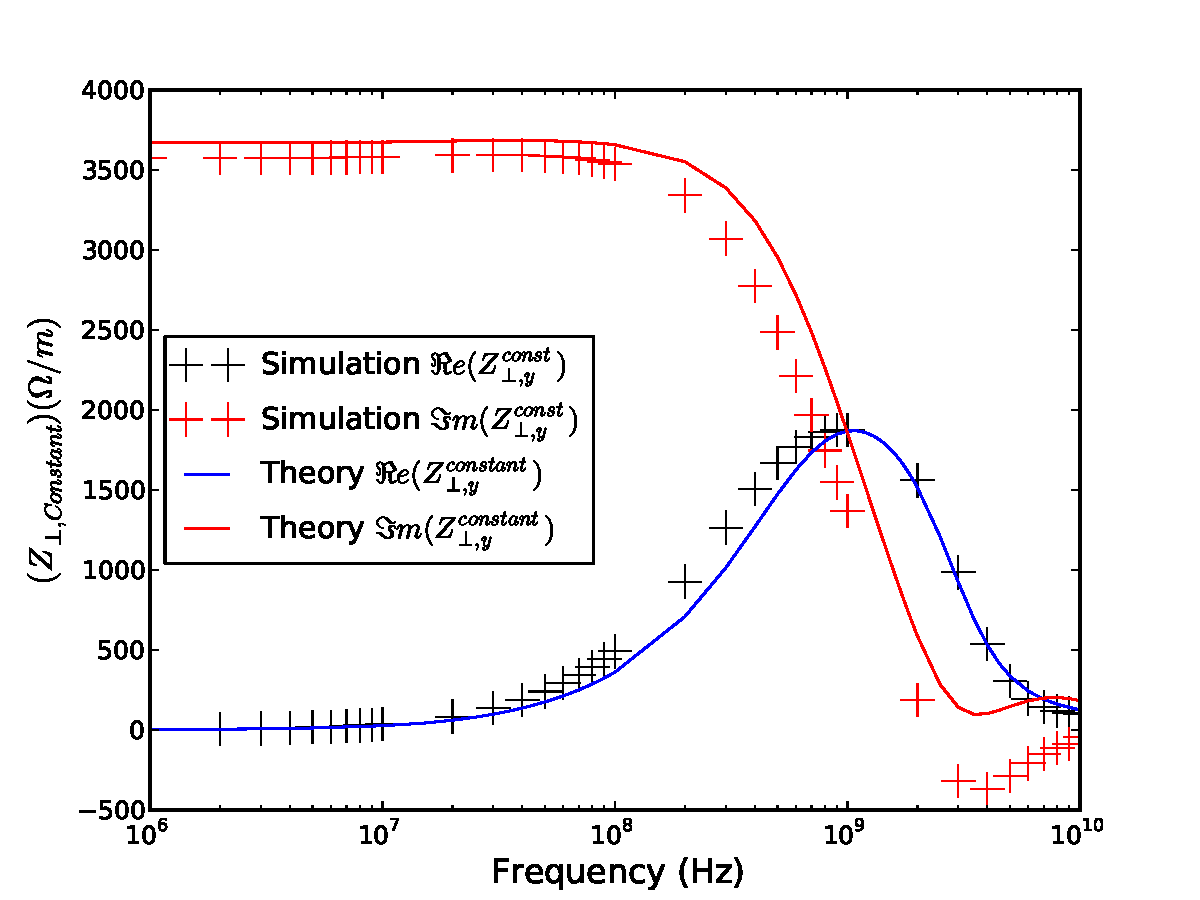
\includegraphics[height=0.35\textwidth]{Bench_Top_Measurements/figures/wire_meas/ferrite-c-core/constant-vertical-impedance.pdf}
\label{fig:c-core-constant}
}
\caption{The impedance of the C-core ferrite kicker as acquired by simulating the classical coaxial wire method in HFSS. Shown is the \subref{fig:c-core-longitudinal} longitudinal impedance, \subref{fig:c-core-dipolar} the dipolar impedance, \subref{fig:c-core-quadrupolar} the quadrupolar impedance and \subref{fig:c-core-constant} the constant transverse impedance.}
\end{figure}

It can be seen that the longitudinal impedance agrees well over the entire frequency range below 1GHz (Fig.~\ref{fig:c-core-longitudinal}). The analytical calculations breakdown above 1GHz due to the family of Bessel functions used for the calculations being optimised for low frequency calculations. Similarly the agreement for the dipolar impedance can be seen to be exceptionally good over the majority of the frequency range, with an increasing descrepency at high frequencies (Fig.~\ref{fig:c-core-dipolar}).

To test the asymmetric method we should look at the constant and quadrupolar terms. In this case it can be seen that the agreement with the constant transverse term is exceptionally good across the entire frequency range (Fig.~\ref{fig:c-core-constant}). The agreement for the quadrupolar impedance is good in the range of frequencies below 1GHz. Above this the unsuitability of the family of Bessel functions used for this frequency range becomes more apparents and the simulated and analytical results diverge.

It can be seen that the proposed asymmetric method can replicate the beam coupling impedance of an asymmetric structure, correctly predicting both longitudinal and transverse (dipolar, quadrupolar and constant) terms below 1GHz. 

\section{High Q-factor Impedances}

For high Q-factor impedances, such as cavity impedances, it is not appropriate to use a coaxial wire method to measure the impedance due to the large perturbation of the boundary conditions that it causes \cite{Masullo:StretchedWire}, in particular below the cut-off frequency of the connecting beam pipes. This is due to the presence of the coaxial wire reducing the cut-off frequency to 0Hz, thus allowing propogation losses at all frequencies rather than just above cut-off. To illustrate this, we can consider the total Q of a cavity to be related to the "trapped" cavity mode Q and the propogation losses as;

\begin{equation}
\frac{1}{Q_{total}} = \frac{1}{Q_{cavity}} + \frac{1}{Q_{prop}}
\end{equation}

During excitation by a charged particle beam, propogation losses do not exist below the cutoff frequency and thus $Q_{prop} = 0$. However, the addition of the coaxial wire causes these propogation losses to occur at all frequencies. Importantly, the Q-factor of these propogation losses is of a similar magnitude or smaller than that of the cavity resonance, leading to a great distortion of the measured Q. Similarly, the perturbation of the conductive wire in the centre of the structure leads to a shift in the resonance frequency of the cavity modes.  This has been well studied in \cite{Masullo:StretchedWire}, an example of which is given in Fig.~\ref{fig:cav-wire-tans}.


\begin{figure}
\subfigure[]{
\includegraphics[width=0.5\linewidth]{figures/cavity_beampipe.pdf}
\label{fig:cavity_beampipe}
}
\subfigure[]{
\includegraphics[width=0.625\linewidth]{figures/cavity_beampipe_coaxial.pdf}
\label{fig:cavity_beampipe_coaxial}
}
\caption{Comparison of the geometries of a cavity and attached beampipes \subref{fig:cavity_beampipe} without and \subref{fig:cavity_beampipe_coaxial} with the coaxial wire in place. Note the dimensions and that the dashed line in \subref{fig:cavity_beampipe} and the solid line in \subref{fig:cavity_beampipe_coaxial} represent the rotational plane of symmetry}
\end{figure}

\begin{figure}
\begin{center}
\includegraphics[width=1.1\textwidth]{Bench_Top_Measurements/figures/coax-trans-cavity.pdf}
\end{center}
\caption{A comparison of the transmission parameters through a pillbox cavity with and without a coaxial wire. A displaced coaxial wire is also shown to illustrate the possibility of exciting dipolar modes also. It can be seen that the transmission signals are drastically changed depending on the presence or not of the wire.}
\label{fig:cav-wire-tans}
\end{figure}

%
%  Things to do for high Q factor measurements
% - Simulation of transmission coefficients with and without coaxial wire
% - Comparison of impedance due to these resonances with time domain simulations
%
%
%
%
%
%
%
%
%
%


%%%%%% Simulations of Beam Impedance %%%%%%%

\chapter{Computational Simulations of Beam Coupling Impedance}
Whilst beam-based measurements and bench-top measurements techniques have been used for some time to measure the impedance of devices and machines, the use of numerical codes to solve 2D and 3D structures is relatively young as a method of identifying the impedance of devices. Recent progress in computational power has now made these a powerful tool in the regime of impedance evaluation. Codes exist that solve simple 2D structures (ECHO2D \cite{Weiland:Echo2d}, ABCI \cite{Chin:ABCI}), 3D structures (CST Particle Studio \cite{cst}, HFSS \cite{hfss}, Maxwell 3D \cite{maxwell}, MAFIA \cite{Weiland:MAFIAv4}) and 3D structures using highly parallelised codes (GdFidl \cite{gdfidl}, ACE3P \cite{Ng:Ace3p}) which allow the simulation of large, complex structures. The codes may be seperated in to two seperate families; time-domain, which calculate the EM fields in a structure by solving Maxwell's equations in the time domain due to a signal inpulse, and frequency-domain which can be used in a number of ways to simulate the beam coupling impedance.

Each of these families of codes has there own relative advantages and disadvantages and peculiarities to use. In this chapter there will a general introduction to a number of the techniques that may be used to calculate the beam coupling impedance from both time-domain and frequency-domain simulations, along with the limitations of each method.
\section{Time Domain Simulations}

Time domain simulations typically rely on direct simulations of the propogation of an EM signal through a structure and evaluating the response in some manner. In this section we shall primarily discuss the use of direct particle beam simulation, that is the simulation of the beams EM profile via a source signal and then subsequently evaluating the trailing field as a result to acquire the wakefield of the source signal and thus the structure simulated.

\subsection{Direct Simulation of a Particle Beam}

A large majority of time domain simulation codes (ECHO, MAFIA, CST Particle Studio, GdfidL) use a method that in effect simulates the passage of a particle beam through the structure and evaluates the subsequent electromagnetic fields in the structure by this signal. This is done in the following way:

\begin{enumerate}
\item{A signal representing the source bunch is defined using a given profile, and then passed through the structure from a defined starting displacement and at a given velocity. Additionally a line of integration is defined along which the witness signal will be taken. This in effect defines a source bunch and a witness particle.}
\item{The simulation is propogated for a given period of time to acquire a significant quantity of the wakefield to correctly analyse the frequency components. It can be seen that for both high-Q resonances and low frequencies this requires a longer wakelength, to encompass the long damping time and correctly resolve the signal frequency, respectively.}
\item{The observed signal is subsequently deconvolved from the source signal to obtain a single particle wakefunction.}
\item{This may then be fourier transformed (using an FFT algorithm or other numerical methods) to acquire the beam coupling impedance.}
\end{enumerate}

These steps are illustrated for clarity in Fig.~\ref{fig:time_domain_beam} using a simple pillbox cavity as an example, using the time domain code CST Particle Studio.

\begin{figure}
\begin{center}
\subfigure[]{
\includegraphics[width=0.45\textwidth]{Computational_Simulations/figures/source-integration-pos.png}
\label{fig:cst_source_signal}
}

\subfigure[]{
\includegraphics[width=0.7\textwidth]{Computational_Simulations/figures/source-witness-signal.png}
\label{fig:cst_wakepotential}
}
\end{center}
\caption{An illusration of the \ref{fig:cst_source_signal} source signal and witness integration in a time domain code. Here a sample from the UA9 goniometer is shown. The source signal and the resulting wakefield are shown in \ref{fig:cst_wakepotential}.}
\label{fig:time_domain_beam}
\end{figure}

It can readily be seen that by defining either the source signal or witness at different displacements it is possible to acquire both the dipolar and quadrupolar impedances. Additional, by taking the gradient of the transverse impedances any constant transverse impedance terms can also calculated.

\section{Frequency Domain Simulations}

There are a number of methods of analysing the beam coupling impedance of a structure using frequency domain simulations. These involve evaluating the structure with no beam present via the use of eigenmode solvers, simulating measurement setups, particularly the coaxial wire technique for systems in which the impedance structure is largely unknown. Finally it is possible to simulate the particle beam also, however this requires a high resolution frequency scan for structures that are expected to be resonant in nature.

\subsection{Eigenmode Simulations}

Eigenmode solvers are a subset of frequency domain solver that are used to identify strongly resonant modes in a structure. These can be cavity modes, antenna like oscillations or a number of other resonances within the structure. The resulting output of the simulation is typically the resonant frequency of the eigenmode(s), the quality factor $Q$ of the mode (if lossy boundary materials are defined) and the field pattern of the eigenmode solution.

From the field pattern it is possible to readily calculate the longitudinal and transverse $R/Q$ of each cavity mode as defined in Sec.~\ref{sec:sec:imp_geo_imp}. The field patterns may also be used to calculate a number of other properties for each eigenmode, such as surface losses and stored energy in the cavity, which will be explained in further details in Sec.~\ref{sec:ferrite_damping}. Further details on this method are available in \cite{Grudiev:LongTransSecCol}

\subsection{The Coaxial Wire Method by Simulation}

The coaxial wire method as described in Sec.~\ref{sec:coax_wire_meth} can be directly simulated using waveguide ports to represent matched connections at the ends of the device under test. The resulting simulations provide a transmission coefficient $S_{21}$ which may subsequently be evaluated in the same manner as measurements made with a physical wire. As with the measurements used in practice, a displaced wire and two wires may be simulated and again treated as measurements. 

\subsection{Simulation of the particle beam}

It is also possible to simulate a particle beam directly in the frequency domain. This is done by defining a wave source that produces a field similar to that of the particle beam. For ultrarelativistic beams this neccessitates a source field that is tangential to the direction of motion, and this may technically be possible for cases in which $\beta < 1$. The field components due to the source may be acquired and are the equivalent of the wakefield contribution at a given frequency. The beam impedance $Z$ can subsequently be easily evaluated from the resulting fields. Further details of this method may be seen in \cite{Kononenko:TransBeamLoading}



%%%%%% Beam Impedance Reduction Techniques %%%%%

\chapter{Beam Coupling Impedance Reduction Techniques}
Due the effects of wakefields on both beam stability and machine equipment it is often necessary to consider the reduction of the beam impedance of different components in particle accelerators. There are a number of ways in which it is possible to reduce the impedance depending on whether the impedance is primarily geometric or material dependent in nature and the most commonly used will be described. Different solutions from mechanical changes in the structures to damping materials placed to damp resonances are discussed. Further references are given to provide more in depth knowledge as required. In particular the use of ferrite to damp cavity modes that may not be removed by redesign, due to either time or mechanical constraints, has recently become a product of intensive study due to the high temperatures seen in many devices that have ferrite placed in them, with concern that the ferrites may heat beyond their Curie temperature during regular operation leading to a deteriorating case for the machine impedance. 
\section{Tapering of Step Transitions}
\label{sec:step_ins}

Although the ideal beam pipe of an accelerator would be of unchanging diameter, it is often necessary to vary the width of the beam pipe for the use of beam instrumentation, insertion devices and machine protection, amongst others. As was shown in Sec.~\ref{sec:imp_geo_imp}, the presence of changes in the pipe diameters gives rise to beam impedance originating at the point of transition. It has been previously demonstrated that this impedance is heavily influenced by the angle of the transition \cite{Podobedov:TaperedImp}, in addition to the frequency of the resonance of the resulting cavity structure. In particular, this has an influence on the "low"-frequency broadband impedance, with gentler slopes causing a reduction in the "low"-frequency impedance. 

There are of course space constraints which restrict the length which tapers may have, both in terms of machine length and the neccessities of size due to the correct operation of the device (for example, collimators or beam instrumentation such as synchrotron radiation monitors). An example of this approach is shown in Fig.~\ref{fig:taper_ex}. This reduction technique has a strong effect of the broadband impedance contribution of a strong resonant impedance caused by step transitions. In particular, it is effective at reducing the imaginary component of the longitudinal beam coupling impedance, as can be seen in the design of the LHC Yellow Book design report for instance \cite{Ruggiero:LHCColEff}. In this case it was determined that all transitions must observe a maximum gradient of 15$^{\circ}$ unless a design requirement neccessitated otherwise.

\begin{figure}
\subfigure[]{
\includegraphics[width=0.45\textwidth]{Beam_Coupling_Impedance_Reduction_Techniques/figures/stepTransitionTaper.png}
\label{fig:taper_geometry}
}
\subfigure[]{
\includegraphics[width=0.45\textwidth]{Beam_Coupling_Impedance_Reduction_Techniques/figures/impedanceTaper.pdf}
\label{fig:taper_impedance}
}
\caption{An example pillbox structure with and without a tapered transition region \ref{fig:taper_geometry}, in this case with the taper at 15$^{\circ}$. The resulting imaginary component of the longitudinal impedances are shown in \ref{fig:taper_impedance}, as these are the most significant for beam stability.}
\label{fig:taper_ex}
\end{figure}


\section{Transition Pieces}
\label{sec:transitions}

Often it is necessary to have transitions in the beam pipe which can not be tapered, either due to space constraints or the operational requirements of the device containing the transition. This a common requirement in devices that require some mechanical freedom of movement (i.e. longitudinal or transverse movement is expected), such as bellows, or electrical isolation from the beam pipe, such as kicker magnets. For these devices it is often possible to use a transition piece, that is one or several pieces of conducting material to screen any transition. These may be rigid or moveable as shown in Fig.~\ref{fig:rf_fingers}, often referred to as RF fingers.

\begin{figure}
\begin{center}
\includegraphics[width=0.45\textwidth]{Beam_Coupling_Impedance_Reduction_Techniques/figures/pimsImage.png}
\label{fig:rf_fingers}
\end{center}
\caption{Example of RF fingers (in this case for the PIMS (Plug In ModuleS) module, placed between cryo-modules in the LHC).}
\end{figure}


This method of impedance reduction is effective for a number of reasons. Firstly it provides a short, good conducting path for the image currents to flow that does not make to the cavity created by the transition visible to the beam, and, in the case of bellows, the image current does not have to follow to long contoured path of the bellows, such as shown in Fig.~\ref{fig:rf_fingers}. This serves to reduce the broadband impedance increase and, by shielding the contours of the bellows, prevents an increase in the imaginary longitudinal impedance due to the increased electrical length of the device. Secondly, by correctly designing the spacing in the transitions, it is possible to minimise field leakage to the surrounding cavities therefore decreasing the visibility of cavity resonances. As an example of a cavity with and without RF fingers and a number of intermediatary steps, see Fig.~\ref{fig:rf_finger_imp}, which illustrates the case of the VMTSA, a vacuum interconnect in the injection region of the LHC \cite{Salvant:VMTSA} containing a double bellow module. It is characterised by a large vacuum chamber (due to the need to contain two circulating beams) with a long set of bellows. The bellows were screened by a long set of RF fingers, which functioned well when good surface contact was maintained between the fingers and the beam pipe. However, when this connection was disrupted (easily created via mechanical stress due to the weak pressure exerted by the afixing spring) the real component of the longitudinal beam coupling impedance increased drastically at around 200MHz, shown by the large decrease in the transmission parameter $S_{21}$ in the case of spring failure, causing further mechanical failure. This highlights the need to correctly consider the mechanical and electromagnetic properties of an impedance reduction system, especially it's possible failure points.


\begin{figure}
\subfigure[]{
\includegraphics[width=0.45\textwidth]{Beam_Coupling_Impedance_Reduction_Techniques/figures/vmtsa-good-contact.png}
\label{fig:vmtsa_operations}
}
\subfigure[]{
\includegraphics[width=0.45\textwidth]{Beam_Coupling_Impedance_Reduction_Techniques/figures/vmtsa-bad-contact.png}
\label{fig:vmtsa_failure}
}
\begin{center}
\subfigure[]{
\includegraphics[width=0.7\textwidth]{Beam_Coupling_Impedance_Reduction_Techniques/figures/vmtsa-impedance.png}
\label{fig:vmtsa_impedance}
}
\end{center}
\caption{The layout of the RF fingers in the VMTSA both in \subref{fig:vmtsa_operations} the fully operational configuration and \subref{fig:vmtsa_failure} when some RF fingers lose contact. \subref{fig:vmtsa_impedance} shows the transmission parameter $S_{21}$ for the VMTSA module with and without good electrical contact between the fingers and the beam pipe as acquired by coaxial wire measurements. Photos and measurements courtesy of J.L. Nougaret.}
\label{fig:rf_finger_imp}
\end{figure}
\section{Conductive Coatings}
\label{sec:conductive_coatings}

As can be seen in Sec.~\ref{sec:res_wall_imp}, a higher conductivity in the material seen by the beam in a particle accelerator results a lower beam coupling impedance. Typically this rule of thumb is followed in the design of particle accelerators, however the operational requirements of devices in the machine often require that they not be made from a good conducting material. Examples of this include collimators (requiring high strength, mechanical stability and certain radiation properties),  beam instrumentation and numerous other devices.

It has been shown \cite{Caspers:ThinCondLayers} that a thin layer of high conductivity material placed on the surface of a poorly conducting material can effectively screen the beam from interacting with the poorly conducting material for a large frequency range. This can be explained by considering the skin depth $\delta$ of a material. As shown in Sec.~\ref{sec:res_wall_imp}, 

\begin{equation}
\delta \left( \omega \right) = \sqrt{\frac{2}{\mu_{0} \sigma \omega}}.
\end{equation}

The skin depth can be thought of as the distance of penetration of the electromagnetic field into the material. It can thus be seen that for a good conducting material like copper ($\sigma_{cu} \approx 6 \times 10^{7} S m^{-1}$), for frequencies of the order of a hundred megahertz or above, a thickness of a $10\mu m$ is larger than the skin depth at 100MHz ($\delta \left( 100\text{MHz} \right) = 6\mu m$), thus effectively screening the layer below. For many machines the part of the frequency spectrum of concern is above 100MHz (most electron machines, small hadron colliders). It is possible to use thicker coatings (on the order of millimetres) for machines that require a very broad frequency range screened. This is investigated in detail in Sec.~\ref{sec:phase-2-col-mat}.


\section{Beam screens in kicker magnets}
\label{sec:beam_screens}

A substantial contributor to the beam coupling impedance in many machines, in both the longitudinal and transverse planes, are kicker magnets. These are magnets that generate a pulsed magnetic field for a limited period of time (i.e. not always on during beam operation as the dipoles and quadrupoles used for beam optics are), often for orbit corrections, extraction and injection. They have been known to be a problematic component of particle accelerators for a number of decades, mostly in lepton machines due to the traditionally higher beam currents that operate in these machines.

In lepton machines they suffered from problems of heating due to eddy currents induced by traversing bunches, and the neccessity that a remedy to this solution maintain the rapid rise time of the magnetic field required for normal kicker magnet operation, which typically requires a field rise time on the order of the bunch or bunch train seperation in a machine \cite{Caspers:ThinCondLayer}. 

A plain ceramic chamber contributes it's own problem from a beam impedance point of view, especially contributing a large imaginary component to the longitudinal impedance due to it's high permitivitty and poor conductivity. In addition it is liable to build up static charges due to being an insulator in a region subject to high electric and magnetic fields. The solution to these problems neccessitates a thin conductive coating on the inside surface of the chamber, either a continuous thin layer (which itself can greatly reduce the field rise time of the kicker magnetic field), or the use of longitudinal stripes, which carry a large proportion of the beam image current, whilst maintaining the rise time characteristics of the magnetic field.

This method will be studied in further depth in Sec.~\ref{sec:mki_studies}, with particular attention to the limitations in use in a high current hadron machine.

\section{Seriagraphy on Kicker Magnets}
\label{sec:seriagraphy}

As described in Sec.~\ref{sec:beam_screens}, kicker magnets are often a substantial contributor towards beam coupling impedance. For many machines they were not foreseen to be a limiting factor to beam operation during construction due to either low beam current, long bunch lengths, large bunch seperations or both. However, with increasing improvements in machine performance, it is possible that they may become a limiting factor, as was the case for the SPS extraction kicker magnets \cite{Kroyer:MKEReduct}. 

For these existing devices, limitations of both time and budget may require the use of retroactive solutions to large beam impedances. Often these must be added to the original equipment, as the continued correct operation of the device requires minimal disruption to the geometry and surfaces of the device. In the case of the SPS extraction kicker magnet (SPS-MKE), the aperture size had to be preserved, as well as the field rise time of the kicker. In this an innovative solution was found - the use of seriagraphy. This entailed the printing of a set of interleaved fingers (see Fig.~\ref{fig:mke_figures}) made from a good conductor (silver), which form a good conductive path for the beam image currents: the ferrite dielectric provides a reasonable capacitive coupling between the interleaved fingers. This serves to replace the broadband impedance typically associated with a ferrite dominated resistive wall impedance with a low broadband impedance, with strong resonant impedances due to the capcitively coupling and physical length of the fingers. The results in the case of the SPS-MKE can be seen in Fig.~\ref{fig:mke_impedance}.


\begin{figure}
\subfigure[]{
\includegraphics[width=0.5\textwidth]{Beam_Coupling_Impedance_Reduction_Techniques/figures/mke-serigraphy-diagram.png}
\label{fig:mke_layout}
}
\subfigure[]{
\includegraphics[width=0.4\textwidth]{Beam_Coupling_Impedance_Reduction_Techniques/figures/mke-serigraphy.png}
\label{fig:mke_picture}
}
\begin{center}
\subfigure[]{
\includegraphics[width=0.4\textwidth]{Beam_Coupling_Impedance_Reduction_Techniques/figures/Printed_comparison_paper.jpg}
\label{fig:mke_impedance}
}
\end{center}
\caption{An example of seriagraphy in the SPS Extraction Kicker Magnets (SPS-MKE). The layout of the interleaved fingers is shown in \ref{fig:mke_layout} and the actual seriagraphed ferrites in \ref{fig:mke_picture}. A comparison of the longitudinal beam coupling impedance with and without the seriagraphy is shown in \ref{fig:mke_impedance}.}
\label{fig:mke_figures}
\end{figure}


\section{Use of damping materials to de-Q resonant caviities}
\label{sec:damping_materials}

For a number of devices it is unavoidable to have a cavity present in the structure. In addition it is often not possible to design the cavity with either tapering or transition pieces due to the need for moveable components; this is the case for a wire scanner or a collimator whose aperture changes with beam parameters. In this case it is necessary to find a way of reducing the beam impedance by altering the properties of resonances. Often it is only the peak value of the impedance attributable to a resonance that is of concern from a beam stability/beam induced heating point of view. 

If we consider the defining properties of a resonant impedance, $f_{res}$, $R/Q$ and $Q$, there are a number of properties that should be noted in changing them. Both $f_{res}$ and $R/Q$ are strongly determined by the geometry of the structure, and thus cannot be significantly modified without possibly neccessitating a modification of the device being altered which may hinder the intended operation. Thus one approach to use is to alter the Q of the resonance. A well known method of altering the Q of a resonant cavity is to add a dispersive or ferritic material to the cavity volume \cite{Klingbeil:ferrCav}, that is a material that has complex permitivitty or permeability , given by $\epsilon_{r} = \epsilon^{'} - j \epsilon^{''}$ and $\mu_{r} = \mu^{'} - j \mu^{''}$ respectively. An example of the permeability of some sample ferrite damping materials is shown in Fig.~\ref{fig:ferr_mu_damp}

\begin{figure}
\begin{center}
\includegraphics[width=0.6\textwidth]{Beam_Coupling_Impedance_Reduction_Techniques/figures/Ferrite8C11.pdf}
\end{center}
\caption{The complex permeability of a sample ferrite of the sort used for damping. In this case 8C11. In use a high $T_{c}$ ferrite is recommended, such as TT2-111R.}
\label{fig:ferr_mu_damp}
\end{figure}

The addition of this family of materials to the cavity has the following effect on the cavity resonances:

\begin{enumerate}
\item{The resonant frequency of any resonance $\omega_{res}$ is reduced by the inclusion of the dispersive material. This can be understood either by considering:}
\begin{itemize}
\item{the $\mu_{r} / \epsilon_{r}$ increasing the effective electrical volume of the cavity by it's inclusion, thereby increasing the effective dimensions of the resonant cavity.}
\item{the RLC equivalent circuit of a cavity resonance, the inclusion of the dispersive material increases either or both of (depending the properties of the material) the inductance and capacitance of the cavity.}
\end{itemize}
\item{The $R/Q$ of the cavity experiences little change. There is a slight modification; either an increase that can be attributed to the increased stored energy in the cavity mode due to $\epsilon^{'} \neq 1$ or a decrease due to the reaaranging field patterns (caused by the incluson of the dispersive material) decreasing the stored energy.}
\item{The $Q$ of the resonance is drastically reduced. This is due to the strong change in the damping time of the resonance due to the addition of the damping material. In terms of cavity properties this can be thought of as the losses in the cavity increasing more rapidly than the stored energy in the cavity.}
\end{enumerate} 

As can be seen, the resulting effect is to drastically reduce the $Q$ of a cavity resonance, and then by the relation $R_{s} = (R_{s}/Q) Q$ it can be seen that the shunt impedance will decrease proportional to $Q$. This reduces the peak of $R_{s}$, but broadens the width of the resonance peak. This indicates two effects of using damping materials as an impedance reduction technique; effects dependent on the shunt impedance $R_{s}$ are suppressed, however effects dependent on the broadband behaviour may suffer negatively as a result. Due to the strong frequency dependent nature of many impedance-driven instability mechanisms and beam-induced heating, these negative side effects rarely outweigh the benefits using damping material in a cavity if necessary.

\subsection{Heat Loads on the Damping Material}

During experience of estimating the heat loads on ferrite damped cavities in high intensity hadron machines (see Sec.~\ref{sec:tctp} for more details), a number of surprising observations were made. In particular the placement of ferrite in a cavity does not always produce a significant reduction in the $Q$ of a resonance and that in such cases the percentage of the power loss in the ferrite was comparatively small compared to conventional wisdom: that in a ferrite damped cavity the majority of power loss would be in the ferrite. It was thus decided to investigate how the addition of a damping material, in this case a ferrous material, to a cavity would alter both the characteristic resonance properties of the cavity and the location of the power load due to interaction with the beam in the cavity.

Two different geometries were used, one of which could be treated analytically to provide a benchmark for the simulation code, and one in which the ferrite is shielded from being directly seen by the traversing beam, as is normally done to reduce the effects of a resistive wall type impedance due to the ferrite. These geometries are shown in Fig.~\ref{fig:ferr_cav_res}. A single eigenmode of each cavity is investigated, both with and without a damping material. 

\begin{figure}
\subfigure[]{
\includegraphics[width=0.45\textwidth]{Beam_Coupling_Impedance_Reduction_Techniques/figures/pillbox_cavity_ferr.pdf}
\label{fig:cav_ferr_no_shield}
}
\subfigure[]{
\includegraphics[width=0.45\textwidth]{Beam_Coupling_Impedance_Reduction_Techniques/figures/pillbox_cavity_shielded_ferr.pdf}
\label{fig:cav_ferr_shield}
}
\caption{Two sample geometries used to examine the effects of ferrite damping material on cavity resonances. \ref{fig:cav_ferr_no_shield} shows a cavity with the ferrite unshielded, and \ref{fig:cav_ferr_shield} shows a more realistic case in which the ferrite is shielded from directly seeing the traversing beam.}
\label{fig:ferr_cav_res}
\end{figure}

For this analysis, a cavity of dimensions $a=60mm$, $b=5mm$, $c=20mm$, made from a material with a conductivity $\sigma = 1.1 \times 10^{6} S m^{-1}$ is used for the simulations of an unshielded cavity. A layer of "ferrite" 0.5mm thick is placed as shown in Fig~\ref{fig:cav_ferr_no_shield}. This material is given the following properties: $\epsilon^{'} = 10$, $\epsilon^{''}/\epsilon^{'} = 0$, $\mu^{'}=1$. $\mu^{''}/ \mu^{'}$ is changed between 0 and 0.2 in steps of 0.02 in order to alter the Q of the resonant mode in incremental steps with the intent of observing how the properties of the cavity change with different scales of damping of the resonance. The "ferrite" is also given a mild conductivity ($\sigma_{ferr} = 10^{-6} S m^{-1}$) as is normal in accelerator ferrites to reduce electrostatic charge build up. 

For the shielded geometry, we use a cavity of the same dimensions as for the unshielded case, with a layer of conductive material 1mm thick placed on the interior of the cavity. A gap of 5mm is left between the beam pipe and the cavity for the beam to couple to the cavity. A ring of ferrite 0.5mm in thickness is then placed on this surface as is shown in Fig.~\ref{fig:cav_ferr_shield}.

Before carrying out the analysis of the location of the heat loss in ferrite, it is prudent to verify that the losses calculated using the field calculator in HFSS are self-consistent and well understood. HFSS calculates two losses internally; the surface loss density and volume loss density. The surface loss density $p_{s}$ is defined in HFSS as

\begin{equation}
p_{s} = \Re{}e \left( \mathbf{S}.\mathbf{n} \right)
\end{equation}

where $\mathbf{S}$ is the Poynting vector and $n$ is the out normal vector to the surface boundary \cite{hfss}. By integrating this over all surfaces the total surface losses in the cavity are obtained. The total wall losses are also given by 

\begin{equation}
P_{loss, wall} = \frac{R_{wall}}{2} \int_{S} \left| \mathbf{H_{surf}} \right|^{2} dS
\label{eqn:wall_losses}
\end{equation}

where $R_{wall}$ is the surface resistance of the wall and $\mathbf{H_{surf}}$ is the surface magnetic field.

HFSS defines the volume loss density $p_{v}$ as 

\begin{equation}
p_{v}=\frac{1}{2}\Re{}e\left( \mathbf{E}.\mathbf{J} + \left( -\mathbf{\nabla} \times \mathbf{E} \right).\mathbf{H} \right) 
\label{eqn:vol_loss_density}
\end{equation}

where again this may be intergrated over all space to obtain the total volume losses. In addition to these methods of calculations of the losses due to the fields in the cavity, it is possible to calculate an equivalent loss of a particle traversing on axis by considering of ohmic losses, with the voltage $V$ that is experienced by the particle traversing the cavity, $R = R_{s}$ the shunt impedance of the cavity resonance and $I$ the beam current. As the eigenmode simulation does not directly simulate a beam, the effective power loss is given by 

\begin{equation}
P_{loss} = \frac{V^{2}}{R_{s}}.
\end{equation}

The surface losses and volume losses are subsequently seperately compared. For the surface losses, the internal surface loss density integrated over all surfaces calculated by HFSS, wall losses as given by Eqn.~\ref{fig:wall_losses} and the equivalent losses of a particle on axis are compared. For this we use the unscreened cavity with no ferrite present to have only surface losses present. The calculated results are shown in Tab.~\ref{tab:surface_losses_ferr}, given in watts normalised to a peak electric field of $1 V m^{-1}$ in the cavity. It can be seen that the two calculations due to the surface fields themselves agree exceptionally well, and the calculation for the equivalent loss of an on-axis particle is agrees to within 20\%. 

\begin{table}
\caption{Comparison of the power loss on the surface of a pillbox cavity by both direct calculation and internal calculation by HFSS (In units normalised to 1V/m maximum electric field)}
\begin{center}
\begin{tabular}{c | c }
Calculation Type & Normalised Power Loss (W)\\ \hline
Direct calculation & 6.2e-10\\ \hline
HFSS internal loss calculations & 6.22e-10 \\ \hline
Loss of an on-axis particle	 & 5.1e-10 \\
\end{tabular}
\end{center}
\label{tab:surface_losses_ferr}
\end{table}

For the volume losses the cavity geometry for the unshielded case is used, with a layer of ferrite 0.5mm thick on inside surface of the cavity. This ferrite has the following material properties; $\epsilon^{'} = 10$, $\epsilon^{'}=0$, $\mu^{'}=10$, $\mu^{"} / \mu^{"} = 0.1$. For this comparison the internal volume loss density integrated over the whole volume as calculated by HFSS, the volume losses using Eqn.~\ref{eqn:vol_loss_density} and the equivalent loss of an on axis particle are calculated, again with loss normalised to a peak electric field of $1 V m^{-1}$ in the cavity. The results are shown in Tab.~\ref{tab:volume_losses_ferr}. It can be seen that the agreement between all three methods of calculating the losses in the cavity is exceptionally good, differing by less than 4\%.

\begin{table}
\caption{Comparison of the power loss in the volume of a pillbox cavity by both direct calculation and internal calculation by HFSS (In units normalised to 1V/m maximum electric field)}
\begin{center}
\begin{tabular}{c | c }
Calculation Type & Normalised Power Loss (W)\\ \hline
Direct calculation & 1.28e-8\\ \hline
HFSS internal loss calculations & 1.29e-8 \\ \hline
Loss of an on-axis particle & 1.33e-8 \\
\end{tabular}
\end{center}
\label{tab:volume_losses_ferr}
\end{table}


The resulting real component of the longitudinal beam coupling impedance for the case of unshielded ferrite is shown in Fig.~\ref{fig:no_screen_long_imp}. The reduction in the resonant frequency and the increase in the peak impedance from the cavity without any damping material to that with is due to the presence of a region of $\epsilon_{r}>1$. Clearly seen can be the effect of the presence of increasing loss tangent of the ferrite, greatly broadening the impedance peak, with the effect of reducing $R_{s}$ of the resonance. The cause of this reduction of $R_{s}$ can be attributed to the reduction in $Q$ for each resonance, as shown in Fig.~\ref{fig:cav_ferr_no_shield_tan_v_q}. It can be clearly seen that the presence of a small piece of ferrite very strongly decreases the Q of a resonance. The corresponding change in the percentage of the power loss in the ferrite itself as the Q is decreased is shown in Fig.~\ref{fig:cav_ferr_no_shield_q_v_loss_ferr}. It can be seen that the power loss is rapidly localised to the ferrite as the Q decreases. To quantify to this power loss: the power loss due to this cavity resonance is calculated assuming a beam with $1.15 \times 10^{11}$ particles per bunch, 288 bunches, a ring circumference 6911m and a bunch length $4\sigma = 0.04m$ assuming a gaussian bunch distribution and that the resonance falls on a beam harmonic, shown in Fig.~\ref{fig:no_screen_loss_tan_v_power}. Here it can be clearly seen that the power loss in the ferrite rapidly converges to the total losses in the cavity, confirming the assumption that most of the power loss for a cavity resonance damped by a damping material is lost in the damping material. 

\begin{figure}
\begin{center}
\includegraphics[width=0.7\textwidth]{Beam_Coupling_Impedance_Reduction_Techniques/figures/no_screen_long_imp_all.pdf}
\end{center}
\caption{The real component of the longitudinal beam coupling impedance of a cavity without and with a damping material with $\epsilon^{'}=10$, $\mu^{'}=10$ and $\mu^{'}/\mu^{'}$ is varied. The non-damped cavity is shown for comparison. The change in resonance frequency and shunt impedance impedance is due to the increased $\epsilon^{'}$ of the damping material.}
\label{fig:no_screen_long_imp}
\end{figure}

\begin{figure}
\subfigure[]{
\includegraphics[width=0.45\textwidth]{Beam_Coupling_Impedance_Reduction_Techniques/figures/no_screen_loss_tan_vs_q.pdf}
\label{fig:cav_ferr_no_shield_tan_v_q}
}
\subfigure[]{
\includegraphics[width=0.45\textwidth]{Beam_Coupling_Impedance_Reduction_Techniques/figures/no_screen_q_vs_loss_ferr.pdf}
\label{fig:cav_ferr_no_shield_q_v_loss_ferr}
}
\caption{\ref{fig:cav_ferr_no_shield_tan_v_q} The reduction in the Q of the cavity resonance with the increasing loss tangent of the ferrite damping, showing a strong decrease of the resonant Q with a small increase in loss tangent. \ref{fig:cav_ferr_no_shield_q_v_loss_ferr} The percentage of the power loss in the ferrite as the resonant Q decreases. this can be seen to tend towards 100\% as the Q approaches 0.}
\label{fig:no_screen_res_alterations}
\end{figure}

\begin{figure}
\begin{center}
\includegraphics[width=0.7\textwidth]{Beam_Coupling_Impedance_Reduction_Techniques/figures/no_screen_loss_tan_vs_power.pdf}
\end{center}
\caption{The power loss due to  a beam with $1.15 \times 10^{11}$ particles per bunch, 288 bunches, a ring circumference 6911m and a bunch length $4\sigma = 0.04m$ assuming a gaussian bunch distribution in the unscreened cavity.}
\label{fig:no_screen_loss_tan_v_power}
\end{figure}

For the case of the shielded ferrite, the real component of the beam coupling impedance is shown in Fig.~\ref{fig:screen_long_imp}. As with the case of the unshielded ferrite, the addition of the damping material causes a decrease in the resonant frequency of the cavity mode, again due to the addition of a material with $\epsilon_{r} > 1$. In addition, the shielding causes a further decrease in the resonant frequency, in this case due to the rearrangement of the field lines due to the changed boundary conditions.

As can be seen from Fig.~\ref{fig:cav_ferr_shield_tan_v_q} the decrease in the Q of the resonance by the increasingly more lossy ferrite follows a similar pattern to that shown by the unshielded structure, as is the increase in the percentage of power loss in the ferrite for the increasing damping of the resonance, shown in Fig.~\ref{fig:cav_ferr_shield_q_v_loss_ferr}. The corresponding change in the power loss in both the cavity as a whole and the ferrite is shown in Fig.~\ref{fig:screen_loss_tan_v_power}. As with the unscreened case, the power lost in the ferrite rapidly converges with the power loss in the entire cavity, indicating that magnetic losses are dominating the losses.	

\begin{figure}
\begin{center}
\includegraphics[width=0.7\textwidth]{Beam_Coupling_Impedance_Reduction_Techniques/figures/screen_long_imp_all.pdf}
\end{center}
\caption{The real component of the longitudinal beam coupling impedance of a cavity without and with shielded damping material with $\epsilon^{'}=10$, $\mu^{'}=10$ and $\mu^{'}/\mu^{'}$ is varied. The non-damped cavity is shown for comparison. The change in resonance frequency and shunt impedance impedance is due to the increased $\epsilon^{'}$ of the damping material.}
\label{fig:screen_long_imp}
\end{figure}


\begin{figure}
\subfigure[]{
\includegraphics[width=0.45\textwidth]{Beam_Coupling_Impedance_Reduction_Techniques/figures/screen_loss_tan_vs_q.pdf}
\label{fig:cav_ferr_shield_tan_v_q}
}
\subfigure[]{
\includegraphics[width=0.45\textwidth]{Beam_Coupling_Impedance_Reduction_Techniques/figures/screen_q_vs_loss_ferr.pdf}
\label{fig:cav_ferr_shield_q_v_loss_ferr}
}
\caption{\ref{fig:cav_ferr_shield_tan_v_q} The reduction in the Q of the cavity resonance with the increasing loss tangent of the ferrite damping, showing a strong decrease of the resonant Q with a small increase in loss tangent. \ref{fig:cav_ferr_shield_q_v_loss_ferr} The percentage of the power loss in the ferrite as the resonant Q decreases. this can be seen to tend towards 100\% as the Q approaches 0.}
\label{fig:screen_res_alterations}
\end{figure}

\begin{figure}
\begin{center}
\includegraphics[width=0.7\textwidth]{Beam_Coupling_Impedance_Reduction_Techniques/figures/screen_loss_tan_vs_power.pdf}
\end{center}
\caption{The power loss due to a beam with $1.15 \times 10^{11}$ particles per bunch, 288 bunches, a ring circumference 6911m and a bunch length $4\sigma = 0.04m$ assuming a gaussian bunch distribution in the screened cavity.}
\label{fig:screen_loss_tan_v_power}
\end{figure}

From these results it can thus be seen that the inclusion of the shielding does not substantially effect the losses due to strong cavity resonances, whilst aiding in reducing the effects of image current flowing through the ferrite (a broadband effect, and thus not considered in the eigenmode simulations). In addition, we see that if the cavity mode is strongly damped by the presence of ferrite (i.e. the $Q$ is reduced by a factor 20 or so) it should be expected that the vast majority of the remaining power lost by particles interacting with the cavity resonance should ultimately be lost in the damping material. 

%%%%%% LHC Collimation Upgrades %%%%%%

\chapter{LHC Collimation Upgrades}
\section{Introduction}

The LHC collimation system is a key part of the machine protection system in the LHC. Due to extremely high stored beam and magnetic energy in the LHC \cite{Schmidt:LHCMP}, amounting to some 160MJ of beam energy and 10GJ of stored magnetic energy, it is neccessary to keep close control on the losses experienced by the system. In the LHC this is done by a combination of monitoring the losses within the machine, carefully controlled losses by the collimation system, and a rigorous interlock system designed to dump the beam safely in the event of the development of dangerous behaviour by the circulating beam \cite{Schmidt:LHCMP}.

The collimation system in the LHC is a four-stage system, composed primarily of primary (TCP), secondary (TCS), and tertiary (TCT) collimators. These serve to scatter the particle halo, then further scatter and absorb the scattered particles. Further protection is provided by absorbers (TCLA), collimators at the injection regions (TCLI and TDI) and at the extraction region (TCDQA). In particular the TCTs are placed near the experimental IPs to protect the inner triplet magnets (used for final focusing of the beam before collision). In total the collimation system is broken down into two IRs; IR3 for betatron cleaning, in which there are:

\begin{enumerate}
\item{1 primary collimator}
\item{4 secondary collimators}
\item{4 absorbers}
\end{enumerate}

per beam and IR7 for momentum cleaning, which is composed of:

\begin{enumerate}
\item{3 primary collimators}
\item{11 secondary collimators}
\item{5 absorbers}
\end{enumerate}

per beam, with an additional 8 tertiary collimators (2 per experimental IP) per beam. In addition to the collimators at the injection and extraction region each beam is exposed to 44 different moveable collimators per circulation of the machine. The primary and secondary collimators presently all have a jaw material carbon reinforced graphite (conductivity $\sigma_{graphite} = 7 \times 10^{4} S m^{-1} $). This material was chosen due to the requirement for a robust jaw material (mechanically stable under large thermal shock) from a machine protection point of view, however not optimised from a beam impedance point of view.

The current collimation system has demonstrated to be exceptionally effective at it's job of providing machine protection to the LHC \cite{Zerlauth:MP}, however it has been shown to be a limiting factor in the luminousity of the LHC due to the large contribution to the transverse beam coupling impedance by the primary, and especially the numerous secondary collimators in the system, which are also almost double the length of the primary collimators. 

\begin{figure}
\subfigure[]{
\includegraphics[width=0.45\textwidth]{LHC_Collimation_Upgrades/figures/longitudinal-rf-fingers-phase-1.png}
\label{fig:phase-1-col-longitudinal-rf}
}
\subfigure[]{
\includegraphics[width=0.45\textwidth]{LHC_Collimation_Upgrades/figures/transverse-rf-fingers-phase-1.png}
\label{fig:phase-1-col-sliding-contacts}
}
\label{fig:phase-1-rf}
\caption{Different components the impedance reduction measures in the phase 1 collimator design. \ref{fig:phase-1-col-longitudinal-rf} shows the longitudinal RF fingers, ensuring a good conducting path for the beam image currents, and \ref{fig:phase-1-col-sliding-contacts} shows the sliding RF contacts on the collimators jaw. These are intended to minimise the volume seen by the beam, thus making any cavity modes that may be excited by the beam at very high frequencies where the beam power spectrum is very small. Images courtesy of A. Bertarelli, CERN.}
\end{figure}

The phase 1 collimator (those presently (as of 2012) in place in the LHC) designs have a number of design features that are designed to reduce the beam coupling impedance of each device. Although the resistive wall contribution to the beam coupling impedance due to the poorly conducting jaw material is significant, the use of longitudinal RF fingers in the transition between the beam pipe to the collimator jaws and of a system of sliding contact fingers to isolate the beam from seeing the collimator vacuum tank (see Fig~\ref{fig:phase-1-rf} for more details). These function well as impedance reduction techniques, however have some limitations from a mechanical point of view. In particular, the sliding contacts have been suspected to be a significant producer of dust in the LHC due to the moving physical contact during collimator alignment. 

Due to these factors (high transverse impedance due to the resistive wall impedance and problems of dust due to sliding contacts) a phase 2 upgrade of the LHC collimation system has been proposed. This entails two components;

\begin{enumerate}
\item{The supplementation of the current secondary collimators (the prime contributor to the large transverse impedance) by a phase 2 design using a good conducting material as the jaw material. There will be some loss of mechnical robustness but it is thought that this will not be detrimental to the requirements of machine protection with a suitable choice of material.}
\item{Replacing the existing sliding RF contacts with a contactless RF system (shown in Fig.~\ref{fig:rf-system-phase-2}). This is designed to remove the problem of dust caused by the sliding RF contacts in the phase 1 system by removing the moving physical contacts. This increase the volume of the cavity visible to the particle beam, decreasing the frequency of the lowest cavity modes. To counteract these new resonances, ferrite is placed in the cavity to decrease the resulting Q of the resonances.}
\end{enumerate}

\begin{figure}
\begin{center}
\includegraphics[width=0.7\textwidth]{LHC_Collimation_Upgrades/figures/cu-geo.png}
\end{center}
\label{fig:phase-2-rf-system}
\caption{The RF system for use in the phase 2 collimation system. The sliding RF contacts of the phase 1 design are replaced with a ferrite damping system. The RF contacts are removed, allowing the beam to see the entire RF cavity, causing resonances at lower frequencies. The Q of these resonances are decreased by the use of ferrite damping tiles.}
\end{figure}

In this chapter shall be presented an comparison of the different jaw materials proposed for use in the phase 2 secondary collimators, in particular a combination of jaw materials aimed at combining extremely robust materials with highly conductive metals, and the results of full 3D simulations of a TCTP collimator - a tertiary collimator for use in the LHC - which is incorporates the ferrite damping system in comparison to the sliding contacts of the phase 1 RF system. 



%
% Introduction to the new collimator design - Old collimator design, problems with sliding rails, new design, new material possibilities
% Material Evaluation - Comparison of CST simulations
% Whole collimator simulations of phase 2 secondary - Transverse and longitudinal modes with ferrite - compared to that from phase 1
% Sims in CST PS, GdFidl and HFSS
% Heating calculations also
%
%
%
%
%



\section{LHC Phase 2 Secondary Collimator Jaw Material}
\label{sec:phase-2-col-mat}

The phase 2 secondary collimators are proposed as an addition to the current phase 1 secondary collimators. They have stringent mechanical requirements, particularly due to the neccessity to withstand impacts by a limited number of bunches in the LHC during injection. In addition they must meet a stringent limit on beam impedance - new devices in the LHC must not increase the total impedance of the machine due to the stability limits imposed due to the existing large transverse and longitudinal impedance. If possible, the effective impedance in the machine should be reduced during operation. The requirements for the material requirements are detailed and summarised in \cite{Bertarelli:Mat}.

To meet the strict requirements of the differing physical requirments on the jaw material, both from a mechanical point view and an impedance point of view, a number of different jaw design solutions have been proposed. These include both single material jaw designs, mixtures of composites and pure metals, and varitiions on a design including ceramic. The proposed jaw material combinations are listed below:

\begin{enumerate}
\item{GlidCop, a copper compositie including aluminium oxide particles. The conductivity is marginally worse than pure copper (see Tab.~\ref{tab:phase2-cond}), but the addition of the aluminium oxide greatly increases the resistance to thermal softening and increases the strength at high temperatures.}
\item{Molybdenum - A metal with good mechanical properties and a conductivity comparable to copper.}
\item{Copper Diamond Composite - A copper composite formed by hot pressing copper with the addition of boron powder and small synthetic diamonds. This is a very mechanically robust material.}
\item{Molybdenum Diamond Composite - As with the above, a molybdenum compositie formed by the use of sintering molybdenum with artificial diamonds.}
\item{Carbon reinforced carbon (CFC) - The current material of the phase 1 secondary collimators. Included for comparison.}
\end{enumerate}

More information on the material choices can be found in \cite{Bertarelli:Mat, Bertarelli:HiRadMat}. The conductivities of the different materials can be found in Tab.~\ref{tab:phase2-cond}. The layouts of the various possible jaw designs can be found in Fig.~\ref{fig:phase-2-jaw-designs}.

\begin{table}
\caption{The electrical conductivity of the different jaw materials proposed for use in the phase 2 design. All results are given for measurements at room temperature (20$^{o}$C)}
\begin{center}
\begin{tabular}{c | c }
Material & Conductivity ($S m^{-1}$) \\ \hline
Glidcop & $5.4 \times 10^{7}$ \\ \hline
Molybdenum & $1.87 \times 10^{7}$ \\ \hline
Copper Diamond Compositie (CuCD) & $1.25 \times 10^{7}$ \\ \hline
Molybdenum Diamond Composite (MoCD) & $5.5 \times 10^{6}$ \\ \hline
Graphite & $7 \times 10^{4}$ \\ \hline
\end{tabular}
\end{center}
\label{tab:phase2-cond}
\end{table}

\begin{figure}
\subfigure[]{
\includegraphics[width=0.45\textwidth]{LHC_Collimation_Upgrades/figures/mo-geo.png}
\label{fig:phase-2-moly}
}
\subfigure[]{
\includegraphics[width=0.45\textwidth]{LHC_Collimation_Upgrades/figures/mo-mocd-geo.png}
\label{fig:phase-2-molycd}
}
\caption{A number of the proposed jaw designs for the phase 2 secondary collimators. \ref{fig:phase-2-moly} shows the jaw made entirely from molybdenum. Glidcop maybe substituted for molybdenum in this design. \ref{fig:phase-2-molycd} shows the jaw made from a mixture of molybdenum diamond composite with a 2mm coating of pure molybdenum on the surface. The composite ensure a mechanically strong jaw, whilst the coating screens the higher resistivity composite and provides a smooth surface on the beam-facing part of the jaw. In this case the composite maybe substituted with copper diamond composite, and likewise the coating may be replaced with GlidCop.}
\label{fig:phase-2-jaw-designs}
\end{figure}

\subsection{Impedance Studies and Analysis}

To analyse the jaw material impedance the Mounet model \cite{Mounet:Flat} for 2D infinite parallel plates is used. This model assumes infinite parallel plates with n-layers of material. It supports non-symmetric structures in addition. The representation of this structure is shown in Fig.~\ref{fig:mounet-model}. For this model we assume a jaw seperation of 4mm (half-width of 2mm), the closest nominal seperation of the secondary collimators and hence a worset-case for beam coupling impedance.

The frequency range of concern is determined by the instability mechanism driving the stability limit in the LHC. It has been demonstrated that this range of concern is from 11.8kHz up to some number of GHz \cite{Metral:phase2Imp} in the transverse plane, driven by loss due to tune spread over an optical resonance. This neccessitates investigating the transverse beam coupling impedance over a very large frequency range, hence the choice of using an analytical method of investigation.

\begin{figure}
\begin{center}
\includegraphics[width=0.85\textwidth]{LHC_Collimation_Upgrades/figures/mounet-model.pdf}
\end{center}
\caption{The physical model of the Mounet model of parallel plate impedance. Note that the two sides of the structure do not have to be symmetric. The materials maybe any material provided it's frequency dependent properties are well defined.}
\label{fig:mounet-model}
\end{figure}

\begin{figure}
\subfigure[]{
\includegraphics[width=0.5\textwidth]{LHC_Collimation_Upgrades/figures/longitudinal.pdf}
\label{fig:phase-2-long}
}
\subfigure[]{
\includegraphics[width=0.5\textwidth]{LHC_Collimation_Upgrades/figures/horizDipolar.pdf}
\label{fig:phase-2-horzdip}
}
\subfigure[]{
\includegraphics[width=0.5\textwidth]{LHC_Collimation_Upgrades/figures/vertDipolar.pdf}
\label{fig:phase-2-vertdip}
}
\subfigure[]{
\includegraphics[width=0.5\textwidth]{LHC_Collimation_Upgrades/figures/horizQuadrupolar.pdf}
\label{fig:phase-2-horzquad}
}
\subfigure[]{
\includegraphics[width=0.45\textwidth]{LHC_Collimation_Upgrades/figures/vertQuadrupolar.pdf}
\label{fig:phase-2-vertquad}
}
\caption{The impedances of different jaw materials for the phase 2 secondary collimators. \ref{fig:phase-2-long} The longitudinal impedance, \ref{fig:phase-2-horzdip} the horizontal dipolar impedance, \ref{fig:phase-2-vertdip}, the vertical dipolar impedance, \ref{fig:phase-2-horzquad} the horizontal quadrupolar impedance and \ref{fig:phase-2-vertquad} the vertical quadrupolar impedance.}
\label{fig:phase-2-jaw-impedances}
\end{figure}

The beam coupling impedances for the various jaw materials is shown in Fig.~\ref{fig:phase-2-jaw-impedances}. From the consideration of the longitudinal impedance, the collimator jaw material is not a significant contirbutor to the machine impedance. The significant concern is the transverse impedance. It can be seen from Figs.~\ref{fig:phase-2-horzdip}, ~\ref{fig:phase-2-vertdip}, ~\ref{fig:phase-2-horzquad}, ~\ref{fig:phase-2-vertquad} that all the potential jaw materials reduce the imaginary component of the transverse impedance (dipolar and quadrupolar) above $10^{3}$ Hz. By comparison with the change in tune shift discussed in Sec.~\ref{sec:tune-shift-bunch-int} it can be seen that this reduces the magnitude of the imaginary component of the tune shift - i.e. the change in betatron tune is reduced. 

Conversely, the peak of the real component of the transverse impedance is moved to lower frequencies as the conductivity of the innermost jaw material increases (shown in greater magnitude for the vertical dipolar impedance in Fig.~\ref{fig:phase-2-vertdip-zoom}). Significantly, this causes the high conductivity jaw materials to present a larger real component of the impedance in the important frequency range from $10^{4}-10^{5}$ Hz. Reviewing Sec.~\ref{sec:growth-time-chrom} it can be seen that this produces an decrease in the growth time of any associated instability. 

\begin{figure}
\begin{center}
\includegraphics[width=0.7\textwidth]{LHC_Collimation_Upgrades/figures/vertDipolarZoom.pdf}
\end{center}
\caption{The real component of the vertical dipolar impedance of the various collimator jaw materials assuming a 2mm half gap.}
\label{fig:phase-2-vertdip-zoom}
\end{figure}

\section{TCTP Impedance Studies}
\label{sec:tctp}

As part of the ongoing collimation upgrade in the LHC, several advances in the LHC design have been proposed. These are as follows:

\begin{enumerate}
\item{For the reasons given in Sec.~\ref{sec:phase-2-col-mat}, the jaw material of the collimators, specifically the secondary collimators, is under review in an effort to reduce the beam impedance, improve cleaning efficiency and continue the present robustness and excellent performance of the LHC collimation system.}
\item{The inclusion of on-collimator BPMs. This is due to the present method of alignment of the collimators, relying on investigating the beam loss patterns in the LHC as a function of collimator aperture, being a very time intensive procedure due to the inherently slow nature of beam loss. The use of on collimator BPMs allows a near instantaneous feedback on the position of the beam relative to the collimator jaw thus greatly reducing collimator setup time \cite{Valentino:ColAlignment, Valentino:BPM}.}
\item{A new RF system (shown in Fig.~\ref{fig:phase-2-rf-system}) to reduce the side effects of the sliding RF contacts used in the phase 1 collimators.}
\end{enumerate}

As part of the upgrade, a series of TCTP collimators shall be installed in the LHC to replace a number of tertiary collimators (TCTs). In total, 8 TCTP and 1 TCSG will be added to the LHC. These collimators are in part intended to act as a test for two of these upgrades, the use of on-collimator BPMs and the new RF system \cite{Dallocchio:ColBPM}. As part of the ongoing effort to limit increases to the LHC machine impedance (shown in Tab.~\ref{tab:lhc-impedance-budget}) and due to continuing concerns about beam-induced heating \cite{Salvant:Heating, Metral:Heating}, all new devices to be placed in the LHC must be examined for both their effect on the beam and as a possibly luminosity limiter. Due to the large number of phase 2 secondary collimators that are planned to be put in the LHC (30 additional secondary collimators to be installed during long shutdown 2) it is vital that the new collimator design, especially the new RF system, is verified for it's efficacy as an impedance reduction technique.  

\begin{table}
\caption{The impedance budgets (both transverse and longitudinal) for LHC at injection and collisions. Taken from the LHC Design Report \cite{Ruggiero:LHCColEff}}
\begin{center}
\begin{tabular}{c | c | c}
Beam Operation & Longitudinal $\Im{}m ( Z_{\parallel}/n )$ $( \Omega )$ & Transverse $\Im{}m ( Z_{\perp} )$ $(M \Omega /m )$\\ \hline
Total Broadband (450GeV) & 0.07 & 1.34 \\ \hline
Total Broadband (7TeV) & 0.076 & 2.67 \\ \hline
\end{tabular}
\end{center}
\label{tab:lhc-impedance-budget}
\end{table}

\subsection{TCTP Collimator - Design and Geometry}

\begin{figure}
\subfigure[]{
\includegraphics[width=0.45\textwidth]{LHC_Collimation_Upgrades/figures/ferrite_circuit.png}
\label{fig:cross-sec-ferr}
}
\subfigure[]{
\includegraphics[width=0.45\textwidth]{LHC_Collimation_Upgrades/figures/rf-fingers.png}
\label{fig:cross-sec-rf-fingers}
}
\caption{The TCTP collimator has a number of important impedance reduction techniques present in its design. Ferrite tiles replace the sliding transverse RF contacts of the phase 1 design, shown in \ref{fig:cross-sec-ferr} (ferrite tiles shown in black) to reduce the resonant Q of the structure. The longitudinal RF fingers, shown in \ref{fig:cross-sec-rf-fingers}, provide a good conducting path for the beam image current in the transition from the beam pipe to the collimator jaw.}
\label{fig:tctp-figure}
\end{figure}

The TCTP is a tertiary type collimator with a jaw made of tungsten. The principle components of interest from a beam impedance reduction point of view are the longitudinal RF fingers that cover the transition from the beam pipe to the collimator structure, and the RF system utilising ferrite blocks and a screen structure, shown in Fig.~\ref{fig:cross-sec-ferr}.

The RF system is designed to work in the following way, where comparison is given to the phase 1 RF system to clarify the differences and the design choices made. The phase 1 sliding contacts adequately masked the surrounding vacuum cavity from the beam, causing the resonant modes of the structure to be dominated by the geometry of the internal structure of the collimator jaw. Due to the small dimensions of this volume the resonant frequencies are thus very high (in the realm of gigahertz) where the beam power spectrum is very small and thus the beam-structure interaction is relatively small thus avoiding both impedance driven instabilities due to cavity modes and beam-induced heating. However the sliding contacts are believed to produce a large quantity of dust which is problematic for beam losses.

Conversely, the TCTP RF system removes the sliding contacts to solve the dust problem. This allows the beam to 'see' the entire vacuum tank of the collimator. This increases the characteristic dimensions driving the resonant frequency modes, thus lowering the minimum frequency of the cavity modes. Hence the frequency of the cavity modes is moved into an area over the beam power spectrum where the spectrum is comparable to the DC beam current in the machine. To counteract this the Q of the cavity modes is reduced by the placement of ferrite tiles in the device to act as a damping material. This strongly reduces the peak height of the impedances thus reducing their effect on both instability and beam-induced heating.
\subsection{Impedance Simulations and Results}
\label{sec:imp-sims-tctp}

The impedance of the TCTP collimator is examined through the use of simulation codes. In order to verify the simulation results it was decided to use both a time domain and a frequency domain code, in this case CST Particle Studio[cite] for the time domain and Ansoft HFSS[cite] for the frequency domain. Due to the reduced simulation time for time domain simulations compared to frequency domain simulations (which must be evaluated mode by mode to correctly evaluate the eigenmodes), the preliminary comparisons are done using the time domain code and the most promising solutions are subsequently investigated in depth using the frequency domain model.

For this comparison we investigate a number of different designs of the RF system for comparison to the ferrite damping solution chosen for construction;

\begin{enumerate}
\item{The phase 1 sliding RF contacts, to provide comparison to the existing RF system. Shown in Fig.~\ref{fig:phase-1-rf}.}
\item{The proposed RF system including the ferrite damping tiles and the RF screen as shown in Fig.~\ref{fig:phase-2-rf-system}.}
\item{The proposed RF system without the ferrite damping tiles. This is too investigate the benefit of including the ferrite tiles.}
\end{enumerate}


\begin{figure}
\subfigure[]{

\label{fig:sliding-contacts}
}
\subfigure[]{

\label{fig:rf-circuit-ferrite}
}
\subfigure[]{

\label{fig:rf-circuit-no-ferrite}
}
\label{fig:rf-systems-tctp}
\caption{The different RF systems considered for the TCTP collimator. \ref{fig:sliding-contacts} shows an RF system similar to the phase 1 RF system. In these simulations the sliding RF contacts are replaced by a perfect connection - for frequencies lower than 2-3GHz this is a good approximation and greatly simplifies the simulation model. \ref{fig:rf-circuit-ferrite} shows the RF circuit complete with ferrite. \ref{fig:rf-circuit-no-ferrite} shows the phase 2 RF circuit but without any ferrite present.}
\end{figure}


The three different systems are shown in Fig.~\ref{fig:rf-systems-tctp}. 



\input{LHC_Collimation_Upgrades/tctp_collimator/transverse_impedance_concerns}
\subsection{Beam-Induced Heating}
\label{sec:beam-heating-tctp}

As seen in Sec.~\ref{sec:imp-sims-tctp}, the longitudinal impedance of the phase 2 RF design indicates a significant number of beam impedance resonances below 1GHz. Although their contribution in the imaginary component of the beam coupling impedance is not significant enough to be of concern from a stability point of view, the resonances may present a problem from the point of view of beam-induced heating. To fully investigate both the effectiveness of the ferrite in damping the cavity resonances and to identify the locations of the power loss, the phase 2 structure is investigated using the frequency domain code HFSS. 

For these simulations we model half of the structure (due to the reflective symmetry in the longitudinal plane), using alternatively perfect E-field (enforcing perpendicular electric fields at the boundary) and H-field (enforcing perpendicular magnetic fields at the boundary) boundary conditions at the symmetry plane to indentify and characterise the eigenmodes up to 2GHz (to cover the majority of the beam spectrum). The structure with and without ferrite is simulated to characterise the effect of the ferrite in damping the cavity modes. Simulations are carried out using the following parameters:

\begin{itemize}
\item{Using a 2$^{nd}$ order basis function solver to ensure good resolution of the fields for R/Q and localised loss calculations.}
\item{The ferrite is assumed to be 4A4, materials data is imported from an external data file and interpolated fit is used between data points.}
\item{We simulate using a single jaw seperation, in this case a half-seperation of 2mm. This is an extremely close jaw seperation, closer in fact than the TCTP collimator would be placed at, but similar to that that the phase 2 collimators would be placed at. This allows some prediction of a worst case scenario for the TCTP and also an analysis of the efficacy of the RF system for the type of operational parameters the phase 2 secondary collimators would be placed at.}
\item{The mesh was auto-generated by the HFSS mesh generator, and run for a convergence criteria of a 0.5\% convergence of the eigenmode frequency between two successive meshes with a 30\% refinement of the mesh between successive solutions.}
\end{itemize}

\begin{figure}
\begin{center}
\includegraphics[width=0.7\textwidth]{LHC_Collimation_Upgrades/figures/longitudinal-impedance-tctp-ferr-freq-dom.pdf}
\end{center}
\caption{The real component of the longitudinal impedance for the TCTP collimator as simulated in the frequency domains for the case with and without ferrite damping tiles. The strong resonances present in the case without ferrite can be seen to be strongly damped when the ferrite tiles are added. However a substantial broadband component occurs in addition due to the broadened resonance peaks.}
\label{fig:long-imp-tctp-freq}
\end{figure}

Here we shall evaluate the resonances as a whole, or a few key resonances from a heating point of view. For a complete listing of the eigenmodes please see App.~\ref{app:tctp-eigenmodes} for a complete breakdown of the TCTP eigenmode simulations. To have a comprehensive review of the heating we consider the following heating possibilities

\begin{itemize}
\item{A beam harmonic occuring exactly on the resonant frequency with a certain bunch profile. Here we consider gaussian and cos$^{2}$ bunch profiles. Parameters for a number of different beam operating modes (summarised in Tab.~\ref{tab:lhc-tctp-heating-para}) are considered.}
\item{Taking theoretical spectra for both 50ns and 25ns bunch spacings. In this case we consider the heating for both nominal operational parameters (1ns bunch length), running conditions from 2012 (bunch length between 1.0-1.5ns) and for HL-LHC parameters. These parameters are summarised in Tab.~\ref{tab:lhc-tctp-heating-para}. Different bunch profiles are considered - gaussian and cos$^{2}$ to account for high frequency lobes observed in measured beam spectra.}
\end{itemize}

\begin{table}
\caption{The LHC operational parameters considered for heating estimates for the TCTP. Operational parameters include the nominal LHC parameters for 25ns bunch spacing, the peak operational intensity for 50ns bunch spacing used in 2012, and the two possible HL-LHC operational schemes, using both 25ns and 50ns bunch spacing. Here the bunch length is assumed to encompass the $4\sigma$ gaussian width.}
\label{tab:lhc-tctp-heating-para}
\begin{center}
\begin{tabular}{c | c | c | c | c }
Operational Mode & $\tau_{b}$ (ns) & $t_{bunch}$ (ns) & $N_{b}$ & $n_{bunches}$ \\ \hline
50ns, 2012 LHC Operation & 1.2 & 50ns & $1.7 \times 10^{11}$ & 1380 \\ \hline
25ns, Nominal LHC Operation & 1.0 & 25ns & $1.15 \times 10^{11}$ & 2808 \\ \hline
HL-LHC 25ns & 1.0 & 25ns & $2.0 \times 10^{11}$ & 2808 \\ \hline
HL-LHC 50ns & 1.0 & 50ns & $3.3 \times 10^{11}$ & 1380 \\ \hline
\end{tabular}
\end{center}
\end{table}

The heating estimates assuming on resonance beam harmonics can be seen in Tab.~\ref{tab:on-res-heating-tctp} for a variety of bunch lengths between 1-1.5ns assuming either gaussian or cos$^{2}$ bunch distributions. The same data for the TCTP without the ferrite damping tiles can be seen in Tab.~\ref{tab:on-res-heating-tctp-no-ferr}. A number of things area immediately evident; The addition of the ferrite drastically reduces the power loss in the TCTP collimator, by a factor of $\approx$ 10. In addition, the consideration of the higher frequency lobes in the heating estimates for the TCTP is significant as can be seen by the large differences (factor $\approx$ 3 between gaussian and cos$^{2}$ profiles). In this case the usefulness for the ferrites is clear.

\begin{table}
\caption{The power loss of a the TCTP collimator with ferrite for a number of operational modes in the LHC and HL-LHC assuming each cavity mode falls upon a beam harmonic. All losses are in watts using the parameters found in Tab.~\ref{tab:lhc-tctp-heating-para}}
\label{tab:on-res-heating-tctp}
\begin{center}
\begin{tabular}{c | c | c | c | c | c | c | c | c  }
$\tau_{b}$ (ns) & \multicolumn{2}{| c |}{50ns, 2012} & \multicolumn{2}{| c |}{25ns nominal} & \multicolumn{2}{| c |}{50ns, HL-LHC} & \multicolumn{2}{| c }{25ns, HL-LHC} \\ \hline
 & $P_{loss, g}$ & $P_{loss, c}$ & $P_{loss, g}$ & $P_{loss, c}$ & $P_{loss, g}$ & $P_{loss, c}$ & $P_{loss, g}$ & $P_{loss, c}$ \\ \hline
1.0 & 2.8 & 7.1 & 5.3 & 15 & 10 & 27 & 16 & 41 \\ \hline
1.1 & 1.9 & 5.1 & 3.6 & 9.8 & 7 & 19 & 11 & 30 \\ \hline
1.2 & 1.4 & 3.7 & 2.5 & 7.0 & 5 & 13 & 7.7 & 21 \\ \hline
1.3 & 0.9 & 2.7 & 1.8 & 5.0 & 4 & 10 & 5.5 & 15 \\ \hline
1.4 & 0.7 & 1.9 & 1.3 & 3.7 & 3 & 7 & 3.9 & 11 \\ \hline
1.5 & 0.5 & 1.4 & 1.0 & 2.7 & 2 & 5 & 2.9 & 8.2 \\ \hline
\end{tabular}
\end{center}
\end{table}

\begin{table}
\caption{The power loss of a TCTP collimator without the ferrite damping tiles for a number of operational modes in the LHC and HL-LHC assuming each cavity mode falls upon a beam harmonic. All losses are in watts using the parameters found in Tab.~\ref{tab:lhc-tctp-heating-para}}
\label{tab:on-res-heating-tctp-no-ferr}
\begin{center}
\begin{tabular}{c | c | c | c | c | c | c | c | c  }
$\tau_{b}$ (ns) & \multicolumn{2}{| c |}{50ns, 2012} & \multicolumn{2}{| c |}{25ns nominal} & \multicolumn{2}{| c |}{50ns, HL-LHC} & \multicolumn{2}{| c }{25ns, HL-LHC} \\ \hline
 & $P_{loss, g}$ & $P_{loss, c}$ & $P_{loss, g}$ & $P_{loss, c}$ & $P_{loss, g}$ & $P_{loss, c}$ & $P_{loss, g}$ & $P_{loss, c}$ \\ \hline
1.0 & 21 & 52 & 41 & 100 & 81 & 197 & 123 & 301 \\ \hline
1.1 & 15 & 38 & 29 & 72 & 56 & 143 & 86 & 218 \\ \hline
1.2 & 10 & 28 & 20 & 53 & 40 & 105 & 61 & 160 \\ \hline
1.3 & 7.7 & 21 & 15 & 39 & 29 & 78 & 43 & 119 \\ \hline
1.4 & 5.4 & 15 & 10 & 30 &20 & 60 & 31 & 91 \\ \hline
1.5 & 4.0 & 12 & 7.3 & 23 & 15 & 46 & 22 & 70 \\ \hline
\end{tabular}
\end{center}
\end{table}

Considering the heating: taking beam harmonics seperated by the inverse of the bunch seperation (40$MHz$ for $t_{bunch} = 25ns$ and 20$MHz$ for $t_{bunch} = 50ns$) we acquire the results presented in Tab.~\ref{tab:heating-beam-harm-tctp-ferr} and Tab.~\ref{tab:heating-beam-harm-tctp-no-ferr} respectively, again for a variety of LHC operational parameters and assuming either a gaussian or a cos$^{2}$ longitudinal bunch profile. In this case it can be seen that the power loss for the ferrite case is larger than that experienced by the case without ferrite. This can be understood due to the fixed frequencies of the beam harmonics - if a high-Q resonance does not occur at or near a beam harmonic then the beam does not couple to the resonance. Due to the broad resonance peaks of the ferrite damped TCTP design the beam may couple to the resonance even if the resonant frequency of the cavity mode does not match the beam harmonic precisely due to the low-Q of the resonance.

\begin{table}
\caption{The power loss of a TCTP collimator with ferrite for a number of operational modes in the LHC and HL-LHC assuming beam harmonics spaced at the reciprocal of the bunch spacing. All losses are in watts using the parameters found in Tab.~\ref{tab:lhc-tctp-heating-para}}
\label{tab:heating-beam-harm-tctp-ferr}
\begin{center}
\begin{tabular}{c | c | c | c | c | c | c | c | c  }
$\tau_{b}$ (ns) & \multicolumn{2}{| c |}{50ns, 2012} & \multicolumn{2}{| c |}{25ns nominal} & \multicolumn{2}{| c |}{50ns, HL-LHC} & \multicolumn{2}{| c }{25ns, HL-LHC} \\ \hline
 & $P_{loss, g}$ & $P_{loss, c}$ & $P_{loss, g}$ & $P_{loss, c}$ & $P_{loss, g}$ & $P_{loss, c}$ & $P_{loss, g}$ & $P_{loss, c}$ \\ \hline
1.0 & 9.5 & 18 & 9.1 & 17 & 36 & 68 & 27 & 53 \\ \hline
1.1 & 7.4 & 14 & 7.1 & 14 & 28 & 55 & 21 & 42 \\ \hline
1.2 & 5.9 & 11 & 5.6 & 11 & 22 & 45 & 17 & 34 \\ \hline
1.3 & 4.8 & 9.6 & 4.5 & 9.2 & 18 & 36 & 14 & 28 \\ \hline
1.4 & 3.9 & 8.0 & 3.7 & 7.5 & 14 & 29 & 11 & 22 \\ \hline
1.5 & 3.2 & 6.6 & 3.0 & 6.3 & 12 & 25 & 9.1 & 19 \\ \hline
\end{tabular}
\end{center}
\end{table}

\begin{table}
\caption{The power loss of a TCTP collimator without ferrite for a number of operational modes in the LHC and HL-LHC assuming beam harmonics spaced at the reciprocal of the bunch spacing. All losses are in watts using the parameters found in Tab.~\ref{tab:lhc-tctp-heating-para}}
\label{tab:heating-beam-harm-tctp-no-ferr}
\begin{center}
\begin{tabular}{c | c | c | c | c | c | c | c | c  }
$\tau_{b}$ (ns) & \multicolumn{2}{| c |}{50ns, 2012} & \multicolumn{2}{| c |}{25ns nominal} & \multicolumn{2}{| c |}{50ns, HL-LHC} & \multicolumn{2}{| c }{25ns, HL-LHC} \\ \hline
 & $P_{loss, g}$ & $P_{loss, c}$ & $P_{loss, g}$ & $P_{loss, c}$ & $P_{loss, g}$ & $P_{loss, c}$ & $P_{loss, g}$ & $P_{loss, c}$ \\ \hline
1.0 & 2.2 & 6.0 & 2.4 & 6.6 & 8 & 22 & 7.2 & 20 \\ \hline
1.1 & 1.5 & 4.2 & 1.6 & 4.5 & 6 & 15 & 4.7 & 14 \\ \hline
1.2 & 1.1 & 2.9 & 1.0 & 3.1 & 4 & 11 & 3.1 & 9.5 \\ \hline
1.3 & 0.8 & 2.1 & 0.7 & 2.2 & 3 & 8 & 2.1 & 6.7 \\ \hline
1.4 & 0.5 & 1.5 & 0.5 & 1.6 &2 & 6 & 1.5 & 4.7 \\ \hline
1.5 & 0.4 & 1.2 & 0.3 & 1.1 & 1 & 5 & 1.0 & 3.5 \\ 
\end{tabular}
\end{center}
\end{table}

A judgement must be made with regards as to which simulations provide a more realistic safety margin for operation in the LHC. For this we must consider both the worst case scenarios in each case and their likelihood. Considering the worst cases in both the cases with and without ferrite we can see that for any given operational mode the worst case for the collimator without ferrite is substantially worse than that with ferrite. Considering the possibility of inaccuracy of the frequencies of the eigenmodes or their Q factors it is typically considered prudent to take the worst case scenario to avoid the need for costly repairs. In the case of adding ferrite it is possible to simply remove the ferrite if it is proved detrimental to operation, therefore present installation plans for the TCTP collimator include the ferrite damping system.

\subsubsection{Location of Power Deposition}

\begin{figure}
\subfigure[]{
\includegraphics[height=0.2\textwidth]{LHC_Collimation_Upgrades/figures/tctp-ferrite-heating.png}
\label{fig:tctp-ferrite}
}
\subfigure[]{
\includegraphics[height=0.2\textwidth]{LHC_Collimation_Upgrades/figures/tctp-rf-fingers-heating.png}
\label{fig:tctp-long-rf-finger}
}
\caption{The different thermally sensitive components of the TCTP collimator highlighted in purple. \ref{fig:tctp-ferrite} shows the ferrite tiles, and \ref{fig:tctp-long-rf-finger} the longitudinal RF fingers.}
\label{fig:tctp-heat-loc}
\end{figure}

Due to the poor cooling available in vacuum (cooled by thermal radiation only. Although surrounded by a housing/in contact with surrounded components, the thermal contact between different components within the collimator is poor) it is important to know the proportion of beam-induced power loss that is lost in thermally sensitive areas. These are areas where large increases in temperature can either lead to direct physical damage (as is the case with RF fingers) or may lead to a worsening physical condition of the collimator (if the ferrite tiles go above their Curie temperature). The components are highlighted in Fig.~\ref{fig:tctp-heat-loc}

The losses on or in different surfaces and volumes is calculated using the loss calculations within HFSS, and then normalised to the total losses in the TCTP structure for each mode. The produces a variety of losses depending on the field pattern of the mode. These are collated in App.~\ref{app:tctp-eigenmodes}. To provide a conservative estimate of the power load we take the highest proportions of power loss of all the modes and assume this is the case for all modes. The percentages for the total device, the ferrite tiles and the longitudinal RF fingers are shown in Tab.~\ref{tab:tctp-heating-loc}. 

\begin{table}
\caption{The percentage of power loss lost in thermally sensitive components in the TCTP.}
\label{tab:tctp-heating-loc}
\begin{center}
\begin{tabular}{c | c}
Component & Percentage of Power Loss \\ \hline
Whole Device & 100 \\ \hline
Ferrite Tiles & 5 \\ \hline
Longitudinal RF Fingers & 4 \\
\end{tabular}
\end{center}
\end{table}

\begin{table}
\caption{The power loss in the ferrite of the TCTP collimator. The most pessimistic of the losses estimated in Tab.~\ref{tab:on-res-heating-tctp} and Tab.~\ref{tab:heating-beam-harm-tctp-ferr} for the 1.0ns case. All losses are in watts using the parameters found in Tab.~\ref{tab:lhc-tctp-heating-para}}
\label{tab:heating-ferr-power-load}
\begin{center}
\begin{tabular}{c | c | c | c | c }
$\tau_{b}$ (ns) & 50ns, 2012 & 25ns nominal & 50ns, HL-LHC & 25ns, HL-LHC \\ \hline
 &  $P_{loss, c}$  & $P_{loss, c}$ &  $P_{loss, c}$  & $P_{loss, c}$ \\ \hline
1.0 & 0.9 & 0.9 & 3.4 & 2.7 
\end{tabular}
\end{center}
\end{table}


The thermal behaviour as a result of this power load can be analysed using design software such as ANSYS \cite{ansys}. The results of these thermal simulations can be seen in \cite{Carra:HeatLoad}, a summary of which is given in Fig.~\ref{fig:tctp-ferrite-temp-rise}. The important figure of merit is whether the temperature of the ferrite increases beyond its Curie temperature. For the TT2-111R, $T_{c}$=375$^{\circ}$C \cite{tt2111r:datSheet}. The power loss for the worst cases of the nominal, HL-LHC and HL-LHC parameters without crab cavities (bunch length $0.5$ns rather than $1.0$ns) is considered, in this case with a factor of two margin of error included to be conservative (i.e. we assume double the power on the ferrite tiles), and it can be seen that the temperature increase for even the worst case results in the temperature being significantly below the Curie temperature for this material.

\begin{figure}
\begin{center}
\includegraphics[width=0.75\textwidth]{LHC_Collimation_Upgrades/figures/temp_increase_tctp_col.png}
\end{center}
\caption{The temperature increase of the ferrite damping tiles in the TCTP collimator under a number of beam operating conditions and for a number of different jaw support materials. Plot taken from \cite{Carra:HeatLoad}.}
\label{fig:tctp-ferrite-temp-rise}
\end{figure}

%%%%%% LHC Injection Kicker Magnet %%%%%%

\chapter{LHC Injection Kicker Magnets}
\label{chap:mki}
The injection kicker magnets in the LHC are part of the injection system for the LHC machine. This system is used to match the trajectory of the injected beam to that of the stable beam path in the accelerator. An example schema for the LHC can be seen in Fig.~\ref{fig:injection-system-schema}. The system typically uses two components: a septum, which may provide a slowly rising and falling time, but strong, field, and kickers, which may provide a rapidly rising and falling, but comparatively weak, field to match the injected beam to the correct trajectory. Similar components are used for the fast extraction of beam (for systems such as the abort system) also.

\begin{figure}
\begin{center}
\includegraphics[width=0.6\textwidth]{LHC_MKI/figures/injection-system.png}
\end{center}
\caption{An example layout of a injection system for an accelerator. Taken from \cite{Barnes:injSys}}
\label{fig:injection-system-schema}
\end{figure}

By design kickers are generally always visible to the beam due to the need to quickly apply their kick. In order to achieve a fast field rise/fall time, the yoke of the kicker magnet is usually a NiZn ferrite. In addition the need for a highly homogeneous field whilst the kick is applied, as well as the strength of the field, neccesitates that the aperture for kickers often be relatively small, meaning they are in close proximity to the beam. This leads to two concerns - that the close proximity of the beam to such a device, that may be made of either a highly lossy material \cite{Day:wireMeasFerr, Barnes:wireMeasKick, Barnes:spsKickerHeating} or a source of strong geometrical impedance \cite{Belver-Aguilar:clicStripline}, may be source of impedance that drives instabilities in the beam \cite{Salvant:spsImpModel}, and secondly that the large real component of the ferrite ferrite may be subject to intense heating in high beam current machines \cite{Barnes:spsKickerHeating}. 

\section{LHC Injection Kicker Magnets}

Each LHC injection kicker magnet (LHC-MKI, or MKI) is a 3m long travelling wave transmission line kicker magnet (ferrite length 2.7m). For LHC there are two injection regions, near IPs 2 (ALICE) and 8 (LHCb), each consisting of a septa system and four MKIs injecting vertically into the machine (The position of the LHC injection systems is shown in Fig.~\ref{fig:lhc-injection-systems}). As a transmission line magnet the magnet is constructed of a c-core ferrite yoke, segmented by alternating HV and ground plates capacitively coupled together by ceramic capacitors to form a magnet of 5$\Omega$ characteristic impedance. The pulse is generated in a pulse forming network (PFN) and is subsequently carried by 10 parallel coaxial cables with a total characteristic impedance of $5 \Omega$, matching the characteristic impedance of the MKI and the PFN. The performance parameters of the magnets rise time, fied strength and homogeneity are given in Tab.~\ref{tab:mki-parameters} \cite{Ducimetiere:mkiSpec}.

\begin{figure}
\begin{center}
\includegraphics[width=0.75\textwidth]{LHC_MKI/figures/injection-points-lhc.png}
\end{center}
\caption{The location of the LHC injection systems in the LHC ring.}
\label{fig:lhc-injection-systems}
\end{figure}


\begin{figure}
\begin{center}
\includegraphics[height=0.4\textwidth]{LHC_MKI/figures/mki-out-vac-tank.png}
\end{center}
\caption{A cross section of an MKI. Visible are the alternating HV and ground plates, seperated by capacitor plates. The HV busbar and the ground return can be seen in the c core of the ferrite yoke.}
\label{fig:lhc-mki-cross-section}
\end{figure}

\begin{table}
\caption{MKI Operational parameters}

\begin{center}
\begin{tabular}{c | c | c}
Number of Kickers per System & 4 & \\ \hline
Kick strength per magnet & 0.3 & T.m \\ \hline
Beam aperture (diameter) & 38 & mm \\ \hline
Characteristic Impedance & 5 & $\Omega$ \\ \hline
Operating charging voltage (PFN) & 54 & kV \\ \hline
Field flat top ripple & < $\pm$0.5 & \% \\ \hline
Field flat top duration & up to 7.86 & $\mu$ s \\ \hline
Field rise time 0.5\%-99.5\% & 0.9 & $\mu$ s \\ \hline
Field fall time 99.5\%-0.5\% & 3.0 & $\mu$ s \\ \hline
Magnet kength & 2.7 & m \\ 
\end{tabular}
\end{center}
\label{tab:mki-parameters}
\end{table}
\subsection{Development of the LHC-MKI Beam Screen}
\label{sec:mki-screen-development}

Concerns about the beam coupling impedance of the SPS extraction kicker magnets (MKEs), and thus beam induced heating with LHC type beam with high current, led to detailed investigation of the SPS kicker magnets \cite{Arduini:beamInducedSPS}. During an extensive measurement campaign, it was deduced that extensive beam-induced heating was due to the large real component of the longitudinal impedance of the MKEs. Subsequently a number of retroactive impedance reduction methods were proposed and evaluated for their effectiveness in decreasing the longitudinal impedance \cite{Kroyer:MKEReduct}.

There had previously been debate on the need for a beam screen for the LHC-MKIs \cite{Vos:beamScreen}: however the beam screen was considered early in the design \cite{Ducimetiere:designMKI}, which ultimately was implemented in the final design \cite{Barnes:improvBeamScreen}. The beam screen is composed of a ceramic tube housing up to 24 screen conductors - conductive wires which extend beyond the length of the ferrite yoke, connected directly to the LHC beam pipe at one end, and capacitively coupled to it at the other. A scheme involving printed conductive strips on the inside surface of the ceramic was tested but was not implemented due to extensive surface electrical breakdown between the strips during pulsing of the kickers. The capacitive coupling is required due to the short rise time requirement of the kicker field - direct connections at both ends would create a short-circuit secondary, causing the characteristic rise time of the system to dramatically increase. In this case electrical simulations indicate that the optimum is with the capacitive coupling at the pulse input end, i.e. the upstream end of the kicker \cite{Barnes:improvBeamScreen}. This will become relevant during the evaluation of heating patterns of the MKI during operation.

The use of the capactive coupling gives rise to a discontinuity of the conducting path of the beam image current. This results in the possibility of exciting resonances in the surrounding structure of the image current path. In this case, resonant modes of a characteristic frequency due to the screen conductors acting as $n \lambda /4$ resonators. To damp these low frequency modes (the screen conductors are some 3m in length), nine ferrite (NiZn) toroids are placed at each end of the beam screen \cite{Caspers:impMeasMKI, Caspera:impMeasLowFreqMKI, Barnes:mkiVacTemp}. Cross sections of the beam screen are shown in Fig.~\ref{fig:beamScreenCross} for clarity.

During testing and conditioning of the MKIs it was discovered than there was still significant surface electrical breakdown/sparking occuring on the outside surface of the ceramic tube during pulsing. Measurements showed that above a PFN voltage of 30kV large quantities of discharge were observed originating from the screen conductors. In particular, the highest induced voltage was known to occur on the screen conductors closest to the HV busbar \cite{Barnes:improvBeamScreen}. Due to the operational voltage requirements, and as it is not feasible to operate the kicker magnets with a PFN voltage below approximately 51kV, a solution had to be found. Following detailed electromagnetic simulations it was decided to remove the screen conductors with the highest induced voltages (those closest to the HV busbar) in an effort to reduce the number of discharges. Removing the 9 screen conductors closest to the HV busbar increased the PFN voltage reached, before discharges began, to 57kV, above the required 54kV to meet the design parameters for the MKI. Measurements demonstrated that this would worsen the longitudinal beam coupling impedance but this was determined to not be large enough to pose a problem from the point of view of beam induced heating \cite{Barnes:improvBeamScreen}.

\begin{figure}
\subfigure[]{
\includegraphics[width=0.3\textwidth]{LHC_MKI/figures/cross_section.pdf}
\label{fig:mkiCrossSec}
}
\subfigure[]{
\includegraphics[width=0.7\textwidth]{LHC_MKI/figures/beamScreenCapEnd.pdf}
\label{fig:beamScreenCapEnd}
}
\caption{Cross sections of the beam screen perpendicular to \subref{fig:mkiCrossSec} and parallel to \subref{fig:beamScreenCapEnd} the direction of beam travel. The screen conductors removed from the majority of the MKIs during the original construction phase are highlighted in red.}
\label{fig:beamScreenCross}
\end{figure}

\subsection{Observations of heating during 2011 and 2012 until Technical Stop 3 (23.09.2012 - 27.09.2012)}

Beginning with the increasing intensity in the LHC during operation in 2011 a number of devices within the LHC were observed to be heating \cite{ Salvant:Heating, Metral:Heating}. Observations and calculations demonstrated a strong relationship between the observed heating and the increasing intensity (first the number of bunches, then the increase in bunch population) indicating that the source of the heating was due to the stored beam interacting strongly with the impedance of many structures - evidenced also by the deteriorating vacuum in some components also. A number of key devices were observed to be exposed to significant heating, in particular devices around the injection region (injection protection collimators, injection kickers, VMTSA (a two beam vacuum interconnect in the injection region in which two beams circulate) and some small insertion devices (ALFA roman pot), as explained at the workshops in Evian in 2011 \cite{Salvant:Heating} and Chamonix 2012 \cite{Metral:Heating}. 

Four PT-100 thermocouples are used for measuring temperatures in each MKI tank, the locations of which are shown in Fig.~\ref{fig:mkiCrossSectionYZ}. The purpose of these PT-100s is to give an indication of the temperature of the ferrite yoke and also of the temperature of the ferrite toroids. Ideally the 2 PT-100s used to indicate the temperature of the ferrite yoke woud be directly in thermal contact with the ferrite; however this is not possible as the ferrite is also pulsed to high voltages. Thus, instead, these two PT-100s are connected to the outermost ground plates, up and down stream. Thus the temperatures measured using these two PT-100s read lower than the actual ferrite yoke temperature. In addition since the magnet is in high vacuum, heat transfer between the different parts of the magnet is not well defined due to the lack of heat transfer via convection, and the complex transfer of heat by conduction and radiation within the magnet structure.

The measured heating of the LHC-MKIs in particular is shown in Fig.~\ref{fig:mki-heating-2011}. Some important notes about the heating can be made, firstly that MKIs 8b and 8d both show high measured temperatures, MKI8d in particular demonstrating much higher measured temperatures, showing temperatures $\approx$20$^{\circ}$C higher than that experienced by the other MKIs. Secondly, that the cooling time to return below the interlock temperature is very long (on the order of 4 hours \cite{Goddard:timeConst}), indicating a large portion of the ferrite yoke is heating, and additionally that the temperature reached was detrimental to magnet operation (i.e. the ferrite yoke was above it's Curie temperature, thus the magnetic field quality was not suitable for injection), hence the necessary cool-down time was substantial enough to affect machine operational schedules. It can also be seen that the peak temperature only gets worse as the beam intensity is increased.

\begin{figure}
\begin{center}\subfigure[]{
\includegraphics[width=1.0\textwidth]{LHC_MKI/figures/mkipt2HeatingBefore.jpg}
\label{fig:mki-ip2-heating-2011}
}
\subfigure[]{
\includegraphics[width=1.0\textwidth]{LHC_MKI/figures/mkipt8HeatingBefore.jpg}
\label{fig:mki-ip8-heating-2011}
}
\end{center}
\caption{The measured temperature of the MKIs at \ref{fig:mki-ip2-heating-2011} IP2 and \ref{fig:mki-ip8-heating-2011} IP8 during 2011 in the LHC. Note MKI8b and MKI8d show significantly higher measured temperatures than the other MKIs.}
\label{fig:mki-heating-2011}
\end{figure}

The temperature of concern in the MKI is that of the ferrite yoke - to ensure that it is below the Curie point - but as mentioned above there are no direct temperature measurement on this component, hence one difficulty in analysing the heating of the MKI is to identify the actual temperature of the ferrite yoke corresponding to the measured temperature. This is a problem which has been analysed in depth in \cite{Barnes:mkiHeating}, in particular inferring the inductance of the magnet under a softstart condition (the pulsing of the magnet with no beam to inject). The softstart is carried out very soon after a beam dump when the ferrite yoke is at its highest temperature. Hence this analysis gives a certain margin of safety to the interlock level, but due to the possible damage that may be done due to a misinjection of the beam a conservative approach is necessary. Thus a few hours of cool down time between injections may still be required.

Prior to technical stop 3 in 2012 there were 2 configurations of the beam screen in the LHC-MKIs - 7 MKIs were in place with 15 (some staggered, some tapered) screen conductors, the 9 screen conductors closest to the HV busbar having been removed due to the electrical breakdown concerns mentioned in Sec.~\ref{sec:mki-screen-development} \cite{Barnes:improvBeamScreen}. A single MKI, MKI8c, was fitted with 24 screen conductors, 15 tapered and 9 shortened screen conductors (trimmed such they do not overlap with the external metallization at the capacitively coupled end). This was to reduce the electric field at the end of the screen conductors closest to the HV busbar, but not significantly improve the beam coupling impedance of the MKI \cite{Barnes:improvBeamScreen}.

\section{LHC Injection Kicker Magnet}

\begin{itemize}
\item{Introduction to the kicker magnet system}
\begin{enumerate}
\item{What are kicker magnets - Injection/Extractions systems}
\item{Why are they potentially a problem}
\end{enumerate}
\item{Explain the background of the LHC-MKI in particular}
\begin{enumerate}
\item{The original concern over heating, subsequent design of the beam screen}
\item{Observed problems with electrical breakdown of the beam screen, and subsequent removal of screen conductors}
\item{Recent observed heating in MKIs}
\end{enumerate}
\item{Summarise current state of the MKIs in the LHC - Beam screen layouts, two sets of kickers, one all of 15 screen conductors, one has one with 24}
\item{Comparison of the measurements and simulations of the LHC-MKI}
\begin{enumerate}
\item{Measurements of the Longitudinal BCI of the MKI - before and after bake out, with 15 and 19 screen conductors}
\item{Measurements of the transverse BCI of the MKI - if time just for interest and as a verification of the asymmetric method}
\end{enumerate}
\item{A breakdown of the impedance that we see in the MKI}
\begin{enumerate}
\item{Start with a simple c - core ferrite magnet}
\item{Add a ceramic tube}
\item{Add screen conductors in internal side - Brief interlude about the limitations this places on the magnet rise time due to creating a Faraday cage}
\item{Add the capacitive coupling - Different lengths of overlap to demonstrate that this controls the frequency of the resonances. Also lengths of the screen conductors for lower resonances}
\item{Add the ferrite damping rings - damp resonances of length of screen conductor - not(!) overlap}
\item{Hopefully show that this is the dominant cause of the resonances}
\end{enumerate}
\item{Summary of different beam screen designs - Where possible include discussion about the reduction of the voltage build up on each screen conductor}
\begin{enumerate}
\item{Screen conductors all of the same length with capactive coupling at one end - Show how increasing the number of screen conductors really helps to reduce the BCI}
\item{Screen conductors with a tapering of the length, with the longest at the side towards the ground plate and the shortest towards the HV plate}
\item{Alternating lengths of long and short screen conductors}
\item{Having the screen conductors in closed slots in the ceramic tube}
\item{The addition of small conducting spheres to the ends of the screen conductors to reduce the high fields at the conductor ends}
\item{Thicker ceramic at the capacitively coupled end of the beam screen to reduce the field gradient}
\item{Alternative beam screen design - Most screen conductor capactively coupled at both ends, with two connected to the beam pipe at one end. Aim to reduce the potential on all conductors by conductively connecting them at the capactively coupled end}
\item{Stepping the external metallization away from the ceramic tube at the ends of the screen conductors. The metallization will be removed and a conducting pipe placed there instead - different step out dstances are investigated}
\end{enumerate}

\item{Heating estimates for all of the above}
\begin{enumerate}
\item{Explain completely the methods of estimating the power losses here - bunch intensity, number of bunches, bunch length, distribution}
\item{Note the benefits of increasing the bunch length for the resonances with 15 screen conductors}
\item{Summary charts of the beam induced heating for the others, and plots illustrating how the changes in bunch length changes the power loss}
\item{Impedance profiles of all of the above - longitudinal predominantly}
\item{Some judgement on which is most appropriate for an impedance point of view}
\item{Comments on the improvements made to existing magnets already - 19 screen conductors}
\end{enumerate}
\end{itemize}
%
% Introduction to kicker magnet systems - PFNs and the materials normally used
% Risks of beam coupling impedance to the kicker magnet system
% Existing beam coupling impedance reduction - ceramic screen with conductive inserts. Limits of this (electrical breakdown)
% First - comparison of simulations to measurements
% Second - Proposals of improvements to the reduction measures - Rounded ends, changing strips arrangements
% Evaluation of new proposals - comparison of heat load (different methods of evaluating heat load (assume crosses resonance, or real spectrum)), explaination of 
% spectrum measurements and the differences bunch length and profile can make
%
%
%



\section{LHC Phase 2 Collimator Designs}
\begin{itemize}
\item{Introduction to the collimator upgrade project - Why are collimators important}
\begin{enumerate}
\item{The have two significant physical requirements - a rigid, sturdy material and must be placed very close to the beam}
\item{The first necessitated the use of graphite/carbon materials for the phase 1 collimators due to their survivability in the condition needed. The second means that the resistive wall impedance is very large}
\end{enumerate}
\item{Phase 2 collimator materials choice}
\begin{enumerate}
\item{Why a phase 2 collimator upgrade?}
\item{Summary of the material requirements and the available materials}
\item{Simple model used - simulations and comparison to analytical models}
\end{enumerate}
\item{TCTP Impedance Studies}
\begin{enumerate}
\item{What is the TCTP? Why do we need it?}
\item{Possibly designs}
\begin{itemize}
\item{Structure with RF fingers isolating the beam from the vacuum tank}
\item{Structure with a narrow connection between central cavity and vacuum tank - simulated with and without ferrite to demonstrate reduction in Q}
\end{itemize}
\item{Simulations Parameters and results}
\item{Heating estimates - using single bunch, multi-bunch, on resonance and equally spaced}
\item{Localisation of the heating - using both CST and HFSS}

\end{enumerate}
\end{itemize}
%
% Introduction to the new collimator design - Old collimator design, problems with sliding rails, new design, new material possibilities
% Material Evaluation - Comparison of CST simulations
% Whole collimator simulations of phase 2 secondary - Transverse and longitudinal modes with ferrite - compared to that from phase 1
% Sims in CST PS, GdFidl and HFSS
% Heating calculations also
%
%
%
%
%



\section{Other Concerns for the MKI Operation and Temperature Reduction}

Given the breadth of concerns that must also be considered alongside beam impedance when discussing the heating of the MKIs, and alterations to the beam screen design, it is suitable to include a brief discussion on these matters here. 

First of the concerns is the transient induced electrical potential on the screen conductors during the pulsing of the kicker magnet. It is due to this high induced voltage (up to 30kV on the conductor closest to the HV busbar during the field rise and -15kV during the field fall) and the resulting surface flashover between screen conductors and to the end of the beam screen, at the capacitively coupled end, that was the initial motivation to remove the 9 screen conductors from the beam screen. A flashover along the surface of the ceramic, from a screen conductor to ground, can result in the MKI field pulse prematurely falling to a low-level, thus mis-kicking some of the bunches being injected. These mis-kicked bunches can cause significant damage to the downstream equipment.

In addition to improving the screening of the ferrite yoke from the beam any proposed beam screen design must also thus allow the magnet to be pusled without electrical breakdown of the screen. Work by Barnes et al \cite{Barnes:eFieldMKI} has found there are a number of factors that can reduce the electric field on the screen conductors. These include the use of spheres on the ends of the screen conductors to reduce the high electric fields at the ends of the screen conductors (Fig.~\ref{fig:mki8d-points}), tapering the length of the screen conductors (Fig.~\ref{fig:24-alternating-length}) and replacing the outer metallization (at the capacitively coupled end) with a cylindrical metal tube with a 1-3mm vacuum gap between the cylinder and the outer surface of the ceramic tube near the ends of the screen conductors (Fig.~\ref{fig:24-step-out-slight}). The aim of this last measure is to remove the external ground from the outside of the ceramic tube, as the metallization has been observed to effectively force the ground plane closer to the screen conductors due to the high permitivitty of the ceramic tube. The effects of these changes on the beam coupling impedance are discussed in later sections.

The second major concern is the transfer of thermal energy out of the kicker magnets, especially from the ferrite yoke. Due to the HV pulsed nature of the kicker magnet operation there is no active cooling within the device, thus cooling is reliant exclusively on thermal radiation of the heat from the ferrite yoke to the vacuum tank. Experiments have shown that the internal surface of the vacuum tank has a very low emissivity in the IR range \cite{Barnes:emisMKI}, and subsequent thermal simulations have shown that the stable temperature of the MKI is very sensitive to the emissivity of the vacuum tank internal surface \cite{Garlasche:2dHeatEmis}. Subsequently a significant quantity of work has been carried out on methods to improve the emissivity of the internal surface of the vacuum tank so as to more effectively passively cool the device, without degrading the ultra-high vacuum within the tank.
\section{Simulations and Measurements of the MKI with 19 Screen Conductors}

As can be seen from Fig.~\ref{fig:mki-ip8-heating-2011}, MKI8d had experienced significantly higher measured temperatures than the other kicker magnets during operation. Analysis of the softstart data for MKI8d shows that $\approx$70$^{\circ}$C measured corresponds to the Curie point ($\approx$120$^{\circ}$C) of the ferrite yoke. Although estimated to experience the same degree of power loss within the structure as the other kicker magnets (due to the similarity of the beam screen layout) the large variation in the emissivity of the internal surface of the vacuum tankhas probably contributed to the higher temperatures observed. As a result of this, and the necessity to find a solution to the high temperatures of the MKIs, in particular MKI8d which was acting as a severe limiter on the integrated luminousity delivered by the LHC, it was decided to implement an improved beam screen in a replacement magnet in an effort to reduce the power loss in this magnet, and at the same time test new features of future beam screen designs.

The following design features were implemented in the replacement MKI8d (explanations are given with the description, see Fig.~\ref{fig:mki8d-points}):

\begin{enumerate}
\item{19 screen conductors are placed within the beam screen in order to improve the shielding of the ferrite from the beam. These are clustered together, with the 5 empty screen conductor slots closest to the HV busbar to limit the maximum induced voltage on the screen conductors. Impedance and electrical simulations have indicated that this will drastically reduce the beam coupling impedance of the MKI, relative to 15 screen conductors. Electrical simulations show that the maximum induced voltage is $\approx$12\% less than with 24 screen conductors \cite{Barnes:mkiElec}.}
\item{Elongated metal spheres are placed on the capacitively coupled end of the screen conductors. These are intended to reduce the field amplification due to any sharp edges at the ends of the screen conductors, thus reducing the possibility of electrical breakdown. This method has some drawbacks due to the need to drill out the slots, using a diamond coated drill, housing the screen conductors to accept the larger elongated spheres.}
\item{The screen conductors are arranged to alternate in length (i.e. there are two lengths of screen conductor in the beam screen) to further reduce the induced potential on the screen conductors. The effect here is for the longer length screen conductors to effectively shield the shorter screen conductors, thus reducing the potential difference between neighbouring screen conductors. This is less effective than tapering the length of the screen conductors, with the shortest length close to the HV busbar. However, for the first prototype it was necessary due to time constraints.}
\item{A preliminary attempt was made to ensure that the emissivity of the inside of the new MKI8d tank was greater than 0.1, by using an ion bombardment technique \cite{Barnes:mkiElec}.}
\end{enumerate}

\begin{figure}
\begin{center}
\includegraphics[width=0.5\textwidth]{LHC_MKI/figures/mki8d-balls.jpg}
\end{center}
\caption{The additional screen conductors and the elongated spheres place in MKI8d to reduce both beam coupling impedance and the electric potential build up.}
\label{fig:mki8d-points}
\end{figure}

Due to the primary motivation for altering the beam screen being the high beam-induced heating seen in the kicker magnets, the impedance studies were primarily motivated by reducing the real component of the longitudinal beam coupling impedance. Simulations carried out prior to the final assembly of the new MKI predicted that the beam-coupling impedance would be strongly reduced by the inclusion of 4 additional screen conductors. Measurements taken of the magnet  confirmed these simulations to very good accuracy, and shown in Fig.~\ref{fig:mki-19-impedance} along with the measurements and simulations for an MKI with 15 screen conductors. It can be seen that the real component of the beam coupling impedance is reduced drastically across the entire frequency range of concern, and the predicted power loss as a result of the simulated impedance (shown in Tab.~\ref{tab:heating-15-19-cond}) shows that the expected power loss in reduced by a factor of 2-3. Calculations of the thermal evolution of the proposed MKI8d replacement also indicated that the maximum temperature reached would decrease significantly ($\approx$30$^{\circ}$C) due to this reduced power load \cite{Garlasche:2dHeatEmis}. 

\begin{figure}
\begin{center}
\includegraphics[width=0.8\textwidth]{LHC_MKI/figures/15_19_sims_measured_comparison.pdf}
\end{center}
\caption{The real component of the longitudinal beam coupling impedance of the reaplcement MKI8d with 19 screen conductors from both simulations and measurements. The corresponding impedance for an MKI with 15 screen conductors is shown for comparison.}
\label{fig:mki-19-impedance}
\end{figure}

\begin{table}
\caption{The power loss due to the impedance calculated for the MKI with 15 (most common configuration) and 19 (as for the newMKI8d) screen conductors. Estimates are given assuming a beam with 1380 bunches, seperated by 50ns, with each bunch containing $1.7 \times 10^{11}$ particles. Estimates of the power loss assuming a gaussian, a parabolic and a cos$^{2}$ longitudinal bunch profile are calculated, and a range given for the lowest (typically the gaussian distribution) and highest (typically the cos$^{2}$ distribution due to the large high frequency lobes) values calculated.}
\label{tab:heating-15-19-cond}
\begin{center}
\begin{tabular}{c | c | c}
Bunch Length (ns) & $P_{loss}$ 15 Screen Conductors & $P_{loss}$ 19 Screen Conductors \\ \hline
1.0 &  134-210 & 50-66 \\ \hline
1.1 &  113-171 & 44-58 \\ \hline
1.2 &  98-143 & 41-52 \\ \hline
1.3 &  86-123 & 40-47 \\ \hline
1.4 &  79-108 & 36-43 \\ \hline
\end{tabular}
\end{center}
\end{table}

\subsection{Temperature of MKI8d after Technical Stop 3}

Due to the promising results of the impedance, electrical and thermal simulations of the proposed MKI8d replacement with 19 screen conductors, it was decided to replace the 15 screen conductor version during technical stop 3 (TS3) \cite{Barnes:emisMKITemp}. It is said the proof is in the pudding, and in this case mine is exceptionally tasty; Fig.~\ref{fig:heating-mki8-post-ts3} shows the temperatures for the kicker magnets at IP8 both before and after TS3. It can clearly be seen that MKI8d (solid red trace) changes from being the magnet with the highest measured temperature in IP8 to the lowest - an excellent confirmation of the understanding of the sources of power loss within the kicker magnet and the thermal evolution due to the power loss. From these very promising results a great deal of confidence in the simulation tools for predicting the beam coupling impedance and the understanding of the causes of the beam coupling impedance were acquired. As such more significant changes to the MKI design maybe investigated using simulation tools with confidence given the good predictions acquired so far.

\begin{figure}
\begin{center}
\includegraphics[width=0.75\textwidth]{LHC_MKI/figures/mki8-temps-post-ts3.png}
\end{center}
\caption{The temperature profile of the IP8 injection kicker magnets during the time period before and after technical stop 3  (TS3), when the MKI8d was changed from a kicker magnet with 15 screen conductors to one with 19 screen conductors. It can be seen this magnet (solid red trace) goes from being the magnet with the highest measured temperature to the magnet with the lowest measured temperature after TS3.}
\label{fig:heating-mki8-post-ts3}
\end{figure}
\section{The Dependence of the Beam Coupling Impedance on the Kicker Components}

As part of the study to improve the beam screen it was decided to investigate systematically the effect of the various components of the kicker magnet on the resulting beam coupling impedance. This is divided into two sections, the study of the effect of the beam screen on the beam coupling impedance of the ferrite yoke, and subsequently a study of the effects of the dimensions of the beam screen and screen conductors on the beam coupling impedance.

\subsection{The Impedance of the MKI - Effects of the Inclusion of the Beam Screen}

To first judge the effectiveness of the concept of the beam screen as an impedance reduction technique we simulate the MKI by systematically adding components to the magnet to determine their effect on the beam coupling impedance. We consider the following configurations of the MKI:

\begin{enumerate}
\item{The c-core ferrite yoke}
\item{The c-core ferrite yoke with a ceramic tube in the aperture}
\item{As "2" above but with 24 screen conductors inserted into the ceramic tube, capactively coupled at one end}
\item{The internal magnet structure including the vacuum tank, HV and ground plates and the surrounding connections}
\end{enumerate}

These geometries are shown in Fig.~\ref{fig:mki-layout-buildup}, and the resulting impedance simulations for the real component shown in Fig.~\ref{fig:mki-buildup-impedance}. Several points can be seen; firstly that the inclusion of the beam screen with screen conductors very effectively screens the beam from the other components of the kicker magnet - including the ceramic tube, the surrounding structures and the ferrite yoke itself. This indicates that for a beam screen in which the ceramic tube holds a large number of screen conductors, the beam is effectively screened from the surrounding structure up to a frequency characterised by the seperation of the screen conductors. This has benefits for the impedance simulations as it is valid to use a reduced simulation model considering just the capacitively coupled end provided we can assume the ferrite is well screened (i.e. we have 24 screen conductors in place). And lastly that the use of the ceramic tube contributes significantly to the imaginary component of the longitudinal impedance of the complete magnet (evidenced by the linear increase of the imaginary impedance, in cases 3 and 4 in the simulation results, with frequency due to the inductive component of the impedance) even with the presence of screen conductors.
 
\begin{figure}
\subfigure[]{
\includegraphics[width=0.45\textwidth]{LHC_MKI/figures/mki-buildup-ferrite.png}
\label{fig:mki-buildup-ferrite}
}
\subfigure[]{
\includegraphics[width=0.45\textwidth]{LHC_MKI/figures/mki-buildup-ferrite-ceramic.png}
\label{fig:mki-buildup-ferrite-ceramic}
}
\subfigure[]{
\includegraphics[width=0.45\textwidth]{LHC_MKI/figures/mki-buildup-ferrite-ceramic-cond.png}
\label{fig:mki-buildup-ferrite-ceramic-cond}
}
\subfigure[]{
\includegraphics[width=0.45\textwidth]{LHC_MKI/figures/mki-buildup-ferrite-ceramic-cond-full.png}
\label{fig:mki-buildup-ferrite-ceramic-cond-full}
}
\caption{The geometries simulated for the various components in the LHC-MKI. These are c-core ferrite only \ref{fig:mki-buildup-ferrite}, c-core ferrite and the ceramic tube \ref{fig:mki-buildup-ferrite-ceramic}, c-core ferrite with the ceramic tube containing 24 screen conductors \ref{fig:mki-buildup-ferrite-ceramic-cond} and finally the complete MKI magnet (without vacuum tank for clarity) \ref{fig:mki-buildup-ferrite-ceramic-cond-full}.}
\label{fig:mki-layout-buildup}
\end{figure}

\begin{figure}
\subfigure[]{
\includegraphics[width=0.5\textwidth]{LHC_MKI/figures/mki-build-up-real-imp.pdf}
\label{fig:mki-buildup-real-imp}
}
\subfigure[]{
\includegraphics[width=0.5\textwidth]{LHC_MKI/figures/mki-build-up-imag-imp.pdf}
\label{fig:mki-buildup-imag-imp}
}
\caption{The \ref{fig:mki-buildup-real-imp} real component and the \ref{fig:mki-buildup-imag-imp} imaginary components of the LHC MKI kicker magnet impedances for different components in the magnet.}
\label{fig:mki-buildup-impedance}
\end{figure}


Concerning the role of the beam screen layout there are two areas to examine - the effect of different quantities of screening of the beam by having more or less screen conductors (in this case removing those directed towards the HV busbar due to concerns of electrical breakdown) and of the effect of different lengths of the screen conductors at the capacitively coupled end of the beam screen.

\subsection{How Screening Changes with the Number of Screen Conductors}

For the changes in the number of screen conductors two variations are carried out - The first is to examine the case of removing several screen conductors in the beam screen towards the HV busbar (shown in Fig.~\ref{fig:mki-take-away-cond-together}). This direction is chosen as these screen conductors experience the highest induced voltage during the pulsing of the kicker magnet, and additionally it was initially thought that on this side the HV busbar would provide some screening of the beam from the ferrite yoke. The second variation is to remove a selection of screen conductors towards the HV busbar (shown in Fig.~\ref{fig:mki-take-away-cond-alt}), in this case to examine whether it is possible to acquire some shielding through using some screen conductors and benefitting from removing some screen conductors to further reduce the rate of electrical breakdown.

\begin{figure}
\subfigure[]{
\includegraphics[width=0.3\textwidth]{LHC_MKI/figures/15-screen-cond.pdf}
\label{fig:15-cond-together}
}
\subfigure[]{
\includegraphics[width=0.3\textwidth]{LHC_MKI/figures/19-screen-cond.pdf}
\label{fig:19-cond-together}
}
\subfigure[]{
\includegraphics[width=0.3\textwidth]{LHC_MKI/figures/24-screen-cond.pdf}
\label{fig:24-cond-together}
}
\caption{Beam screens with different numbers of screen conductors removed from the design quantity of 24. Models of 15 \ref {fig:15-cond-together}, 19 \ref{fig:19-cond-together} and 24 \ref{fig:24-cond-together} screen conductors are considered for the impedance simulations. Conductors surrounded by the boxes are removed in this case.}
\label{fig:mki-take-away-cond-together}
\end{figure}

\begin{figure}
\subfigure[]{
\label{fig:17-cond-alt}
\includegraphics[width=0.45\textwidth]{LHC_MKI/figures/17-cond-alt.pdf}
}
\subfigure[]{
\includegraphics[width=0.45\textwidth]{LHC_MKI/figures/19-cond-alt.pdf}
\label{fig:19-cond-alt}
}
\subfigure[]{
\includegraphics[width=0.45\textwidth]{LHC_MKI/figures/20-cond-alt.pdf}
\label{fig:20-cond-alt}
}
\subfigure[]{
\includegraphics[width=0.45\textwidth]{LHC_MKI/figures/24-cond-alt.pdf}
\label{fig:24-cond-alt}
}
\caption{Beam screens with different numbers of screen conductors removed from the design quantity of 24. Models of 17 \ref {fig:17-cond-alt}, 19 \ref{fig:19-cond-alt}, 20 \ref{fig:20-cond-alt} and 24 \ref{fig:24-cond-alt} screen conductors are considered for the impedance simulations. Conductors that are coloured red are the removed in each case.}
\label{fig:mki-take-away-cond-alt}
\end{figure}

\begin{figure}
\subfigure[]{
\includegraphics[width=0.5\textwidth]{LHC_MKI/figures/mki-no-screen-conductors-real-impedance.pdf}
\label{fig:remove-cond-real-imp}
}
\subfigure[]{
\includegraphics[width=0.5\textwidth]{LHC_MKI/figures/mki-no-screen-conductors-imag-impedance.pdf}
\label{fig:remove-cond-imag-imp}
}
\caption{The longitudinal impedance of the MKIs with different numbers of screen conductors included in the beam screen. Shown is the real component \ref{fig:remove-cond-real-imp} and the imaginary component \ref{fig:remove-cond-imag-imp} of the longitudinal impedance.}
\label{fig:remove-cond-impedance}
\end{figure}

The longitudinal impedance for these configurations is shown in Fig.~\ref{fig:remove-cond-impedance}. It can be seen that for both components of the impedance that more screen conductors reduces the magnitude of the impedance at all frequencies - this can simply be understood as improving the screening of the ferrite yoke from the beam with additional screen conductors. This can particularly be seen in the increase of the number of screen conductors from 15 to 19 to 24 conductors in total - The screening is improved dramatically in each subsequent case. 

In addition it can be seen that it is preferable to distribute the screen conductors such that the maximum arc of the beam screen without screen conductors is minimised. This can clearly be seen by comparing the case of 19 screen conductors where all conductors are clustered together (as was done for the replacement MKI8d (Fig.~\ref{fig:19-cond-together}) and for 19 screen conductors, where only 3 are missing close to the HV busbar (Fig.~\ref{fig:19-cond-alt}). Again this advantage is bourne out in the power lost in the structure. This is however not beneficial without consideration of the induced electric field during kicker pulsing, as the induced voltage on a given screen conductor is still the same, and thus surface flashover along the ceramic tube to the external metallization is not changed by this layout. It can thus be seen that the beam screen design itself must be optimised with regards to the induced screen conductor voltage before more conductors can be added to the ceramic tube to improve screening.

\subsection{Dependence of the Impedance on the Beam Screen Dimensions}

It will now be shown that with 24 screen conductors placed in the ceramic tube that the resulting impedance is dominated by the dimensions of the ceramic tube, the screen conductors and the external metallisation at the capacitively coupled end of the beam screen. To investigate how changes to certain parameters (specifically the length of the overlap between the screen conductors and the external metallization and the thickness of the ceramic tube) a cut down model of the kicker magnet is used, considering just the capactively coupled end of the kicker magnet (shown in Fig.~\ref{fig:cut-down-mki-cap-end}). This is done to allow a larger mesh density in this important (from the electrical and impedance point of view) region of the kicker magnet. In models of the full kicker magnet the mesh density is severely limited due to the large mesh generated in the entire magnet volume which subsequently may make the mesh very limited in near beam areas (for example in the ceramic tube between the screen conductors and the external metallization. A comparison of the meshes is shown in Fig.~\ref{fig:mki-mesh-com-cst}). 

\begin{figure}
\begin{center}
\includegraphics[width=0.75\textwidth]{LHC_MKI/figures/cutDownModel.png}
\end{center}
\caption{The cut down simulation model used for simulations of the MKI beam screen with 24 screen conductors.}
\label{fig:cut-down-mki-cap-end}
\end{figure}

\begin{figure}
\subfigure[]{
\includegraphics[width=0.45\textwidth]{LHC_MKI/figures/meshLarge.png}
\label{fig:mesh-full}
}
\subfigure[]{
\label{fig:mesh-cutdown}
\includegraphics[width=0.45\textwidth]{LHC_MKI/figures/meshCutDown.png}
}
\caption{A comparison of the mesh that may be generated in CST Particle Studio using both the full model \ref{fig:mesh-full} and the cutdown model \ref{fig:mesh-cutdown}. Not the greatly increased mesh density in the important overlap region between the screen conductors and external metallization. The simulation time for the first is on the order a day, for the second 30 minutes.}
\label{fig:mki-mesh-com-cst}
\end{figure}

First we shall consider the effect the impedance for different lengths of overlap of the capacitively coupled sections. To do this we consider just the end section, and change the length of the external metallization to change the length of the overlap (the length of the screen conductors used is keep fixed to avoid changing any potential resonances due to the modelled length of the screen conductors acting as $\lambda /4$ resonators). Overlaps of between 0.08m and 0.12m at 0.01m intervals are simulated, and the results shown in Fig.~\ref{fig:overlap-imp}. It can be seen that each overlap has a distinct set of resonance frequencies. The source of these resonances can be seen to be the result of the overlap between the external metallization and the screen conductor acting as a $n \lambda /2$ resonator. End effects caused the effective length of the overlap to be extended to some degree, which fitting to the resonance frequencies has shown to be $\approx 9$mm for all lengths for a ceramic tube thickness of 7mm. This gives a resonant frequency $f_{res}$ of

\begin{equation}
f_{res} = \frac{nc}{\sqrt{\epsilon_{r}}2 \left( L_{overlap} + \delta_{fringe} \right)}
\label{eqn:imp-overlap-fres}
\end{equation}

where $n$ is an integer, $c$ is the speed of light $\epsilon_{r}$ is the relative permitivitty of the volume material ($\epsilon=10$ for the alumina beam screen), $L_{overlap}$ is the length of overlap and $\delta_{fringe}$ is the effective increase in length due to fringe fields. The resonant frequency calculated using Eqn.~\ref{eqn:imp-overlap-fres} is shown for the first resonances for all the effective lengths of overlap in Fig.~\ref{fig:overlap-imp-zoom}, and up to 2.5GHz for the case of the overlap being 100mm in Fig.~\ref{fig:imp-overlap-fres}. It can be seen that the predicted resonant frequencies match the simulated very well. Work is still under way as to how to determine the peak impedance of each resonance. In addition predictions for the power loss due to the impedances for different effective overlaps calculated assuming either a broadband heating scenario or assuming a beam harmonic at the resonant frequency as shown in Tab.~\ref{tab:heating-overlap}. It can be seen that changing the length of the overlap does not strongly correlate to the change in power loss assuming a broadband heating scenario. It can be seen that increasing the length of the effective overlap causes an increase in the power loss assuming a resonant heating scenario, but this correlation is not clear as there is much variance in the values.

\begin{figure}
\subfigure[]{
\includegraphics[width=0.5\textwidth]{LHC_MKI/figures/mki-overlap-len-real-imp.pdf}
\label{fig:overlap-imp}
}
\subfigure[]{
\includegraphics[width=0.5\textwidth]{LHC_MKI/figures/mki-overlap-len-real-imp-zoom.pdf}
\label{fig:overlap-imp-zoom}
}
\caption{\ref{fig:overlap-imp} The real component of the longitudinal beam coupling impedance for different lengths of the overlap, and \ref{fig:overlap-imp-zoom} a zoomed in plot of the first resonances of all the overlaps with the calculated resonance frequency for each based on the effective length. For each the thickness of the ceramic tube is 7mm.}
\label{fig:mki-overlap-imp-tot}
\end{figure}

\begin{figure}
\begin{center}
\includegraphics[width=0.6\textwidth]{LHC_MKI/figures/mki-overlap-fres-100mm.pdf}
\end{center}
\caption{The impedance of the beam screen with 24 screen conductors with an overlap $L_{overlap}=100mm$ and the predicted resonance frequencies from Eqn.~\ref{eqn:imp-overlap-fres} shown as vertical lines.}
\label{fig:imp-overlap-fres}
\end{figure}

\begin{table}
\caption{The beam induced heating calculated for a number of beam screen designs with 24 screen conductors with equal thickness of ceramic tube (thickness of 7mm) with different effective overlaps assuming 50ns bunch spacing LHC conditions (1380 bunches, $1.7\times 10^{11}$ppb with a bunch length of 1ns). It can be seen that the broadband heating component is relatively constant for the change in overlap, whilst the resonant component only significantly changes with a large increase in the effective overlap.}
\label{tab:overlap-heating}
\begin{center}
\begin{tabular}{c | c | c | c | c}
Overlap (mm)& \multicolumn{2}{c |}{LHC, 50ns, 1.7e11ppb} & \multicolumn{2}{|c}{LHC, 25ns, 1.15e11ppb} \\ \hline
 & BB (W) & Res(W) & BB (W) & Res (W) \\ \hline
80 & 38.5 & 6.9 & 30.0 & 13.0 \\ \hline
90 & 39.1 & 6.9 & 31.0 & 13.1 \\ \hline
100 & 35.3 & 12.1 & 28.8 & 23.0 \\ \hline
110 & 36.1 & 13.1 & 31.6 & 24.9 \\ \hline
120 & 36.7 & 12.7 & 28.9 & 24.1 \\ 
\end{tabular}
\end{center}
\end{table}

Secondly the influence of the thickness of the beam screen is considered. This is a concern as increasing this thickness has two effects - to change the value of the capcitance at the capacitively coupled end which effects the low frequency impedance, and the increase in the volume of the overlap region due to the increased thickness. The internal diameter of the ceramic tube is kept at 42mm, whilst external diameters of 50, 53 and 56mm are considered, giving tube thicknesses between 4 and 7mm. The resulting real component of the longitudinal impedances is shown in Fig.~\ref{fig:tube-thickness-imp}, where it can be seen that increasing the ceramic tube thickness has two effects - a slight lowering of the resonant frequency, but also a significant increase of the peak impedance of the resonance, by almost a factor 2 from a tube 4mm thick to a 7mm thick tube. The difference that the peak impedances make to the expected heating of the MKI can be seen in Tab.~\ref{tab:thickness-heating}, where it can be seen that the change in the power loss due to the increased thickness could be expected to be small assuming a broadband heating scenario, but increases significantly if we assume a beam harmonic falls upon the resonant frequency.

The small reduction in the resonant frequency as the thickness of the ceramic tube is increased is expected as the fringe fields will increase with greater thickness. The examination of the prediction shows that the increase in effective length, due to a non-zero thickness of the ceramic tube, is given (for $\epsilon_{r}$=10 for all frequencies) by an increase in effective length (in mm) of $\approx$ 0.0125$\times$thickness (in mm).

\begin{figure}
\begin{center}
\includegraphics[width=0.5\textwidth]{LHC_MKI/figures/mki-tube-thickness-real.pdf}
\end{center}
\caption{The variance of the real beam coupling impedance with the tube thickness. External diameters of 50, 53 and 56mm correspond to tube thicknesses of 4, 5.5 and 7mm respectively. The physical overlap is 100mm in all cases.}
\label{fig:tube-thickness-imp}
\end{figure}

\begin{table}
\caption{The beam induced heating calculated for a number of beam screen designs with 24 screen conductors of equal length (overlap of 100mm) with different tube thicknesses assuming 50ns bunch spacing LHC conditions (1380 bunches, $1.7\times 10^{11}$ppb with a bunch length of 1ns). It can be seen that the change in broadband heating component does not strongly correlate with the change in tube thickness, whilst the resonant component can increase drastically due to the increasing peak impedance as a result of increasing the tube thickness.}
\label{tab:thickness-heating}
\begin{center}
\begin{tabular}{c | c | c }
Outer Tube Diameter/Tube Thickness (mm)  & $P_{loss, BB}$ & $P_{loss, Res}$ \\ \hline
50/4  & 30 & 4 \\ \hline
53/5.5  & 26 & 10 \\ \hline
56/7  & 35 & 12 \\ 
\end{tabular}
\end{center}
\end{table}


\section{New Beam Screen Designs}

Using the knowledge acquired from examining the beam coupling impedance dependence on the layout of the beam screen from the previous section, and additionally the electrical field simulations of the induced voltages on the screen conductors during magnet pulsing, a number of alternative beam screen designs have been proposed. The driving points in these designs has been to reduce the power loss into the MKI (in this case to reduce the temperatures reached by the ferrite yoke) and to reduce the surface eletric field of the ceramic tube, by the end of the screen conductors during magnet pulsing to further reduce surface flashover between the screen conductors and along the ceramic tube to a ground plane.

The proposed designs are described below:

\begin{itemize}
\item{24 screen conductors of alternating length, as shown in Fig.~\ref{fig:24-alternating-length}. The alternating length screen conductors layout has been demonstrated to reduce the surface electric field associated with the shorter length screen conductors, thus being beneficial to the electrical breakdown rate of the shorter conductors. However the electric field associated with the longer screen conductors is increased.}
\item{24 screen conductors tapered in length, as shown in Fig.~\ref{fig:24-tapered-length}. The tapering of the screen conductors has previously been shown to help reduce the surface electric field of the shorter conductors in designs with 15 screen conductors.}
\item{24 screen conductors some with an alternating length and then tapered towards the HV busbar, as shown in Fig.~\ref{fig:24-alternating-tapered}. This mixture of the above two designs is intended to use the reduction of surface electric field of the shorter conductors due to the tapering, whilst keeping a relatively high capacitance at the capacitively coupled end so as to not induce additional worse resonances here. Note that the alternating length screen conductors are closest to the return busbar and hence have the lowest induced voltage: hence an increase in the electric field of the longer conductors is no so important an effect.}
\item{24 screen conductors in enclosed slots in the ceramic tube, as shown in Fig.~\ref{fig:24-enclosed-slots}. The intention of this design is to increase the necessary induced voltage on the screen conductors before breakdown occurs, because surface flashover is no longer a possile breakdown path. This possible solution is discounted because of extreme difficulties associated with the manufacture of the ceramic tube.}
\item{An alternative screen conductor layout, in which two conductors are conductively connected to ground at one end and all others are capacitively coupled to ground at both ends \cite{Barnes:mkiAlt}, as shown in Fig.~\ref{fig:alt-screen-design}. This design is intended to reduce the induced voltage on the screen conductors by having all the screen conductors be connected to one another at the capacitively coupled end thus receiving the same induced voltage. To counter possible longitudinal eddy currents during pulsing reducing the field rise time, the majority of the screen conductors are capacitively coupled at both ends of the magnet, with two conductors conencted to ground at the downstream end of the magnet.}
\item{24 alternating length screen conductors with part of the metallization replaced by a external metal cylinder, as shown in Fig.~\ref{fig:24-step-out-slight}. This design is intended to reduce the electric field at the capacitively coupled end by replacing the metallization on the external surface of the ceramic tube close to the ends of the screen conductors, with a metal cylinder some millimetres off the ceramic tube outer surface. Electric field simulations had shown that the high permittivity of the ceramic was in effect pushing the ground plane into the ceramic tube, reducing the effective spacing between the screen conductors and the metallization, whereas this physical air gap should reduce this effect \cite{Barnes:mkiAlt}.}
\item{24 screen conductors of a mixture of alternating and tapered lengths with part of the metallization replaced with an external metal cylinder \cite{Barnes:mkiElecSurfCer}, as shown in Fig.~\ref{fig:24-final-design}. This was intended to improve on the above design by using the combined alternating and tapered design to further reduce the electric field on the surface of the ceramic tube associated with the screen conductors. Due to difficulty of manufacturing the step out of the beam screen is continued to the end of the ceramic tube. \textbf{This is the proposed final design for implementation in the replacement MKIs for installation during long shutdown 1}.}
\end{itemize}

\begin{figure}
\begin{center}
\includegraphics[width=0.7\textwidth]{LHC_MKI/figures/mki-design-layouts/alternating_screen_conductors.pdf}
\end{center}
\caption{A MKI beam screen design with alternating lengths of screen conductors - with a difference in length b.}
\label{fig:24-alternating-length}
\end{figure}
\begin{figure}
\begin{center}
\includegraphics[width=0.7\textwidth]{LHC_MKI/figures/mki-design-layouts/shortening_screen_conductors.pdf}
\end{center}
\caption{A MKI beam screen design with tapered lengths of screen conductors. The taper may be altered to acquire the desired combination of impedance and surface electric field on the ceramic tube.}
\label{fig:24-tapered-length}
\end{figure}
\begin{figure}
\begin{center}
\includegraphics[width=0.7\textwidth]{LHC_MKI/figures/mki-design-layouts/combination_layout.pdf}
\end{center}
\caption{A MKI beam screen design with a combination of tapered and alternating screen conductors. The degree of alternating and tapering may change dependent of the desired impedance and surface electric field associated with the screen conductors. The alternating length conductors are closest to the return busbar.}
\label{fig:24-alternating-tapered}
\end{figure}

\begin{figure}
\begin{center}
\includegraphics[width=0.7\textwidth]{LHC_MKI/figures/mki-design-layouts/enclosed_diagram.pdf}
\end{center}
\caption{A MKI beam screen design with enclosed slots (shown in comparison to the usual beam screen design with open slots) for the screen conductors.}
\label{fig:24-enclosed-slots}
\end{figure}

\begin{figure}
\begin{center}
\includegraphics[width=0.7\textwidth]{LHC_MKI/figures/mki-design-layouts/alternative_screen_design.pdf}
\end{center}
\caption{A MKI beam screen design using an alternative screen conductor layout in which 2 (cross section shown here) conductors are connected to ground at the downstream end of the screen, and all conductors are connected together at the other end. Both ends have capacitive coupling.}
\label{fig:alt-screen-design}
\end{figure}

\begin{figure}
\begin{center}
\includegraphics[width=0.7\textwidth]{LHC_MKI/figures/mki-design-layouts/alternating_screen_conductors_step_out_metallisation.pdf}
\end{center}
\caption{A MKI beam screen design implementing a replacement of some of the external metallization with a metallic cylinder so as to remove the ground plane closest to the ends of the screen conductors from the outer surface of the ceramic tube.}
\label{fig:24-step-out-slight}
\end{figure}

\begin{figure}
\begin{center}
\includegraphics[width=0.7\textwidth]{LHC_MKI/figures/mki-design-layouts/mki-final-design.pdf}
\end{center}
\caption{The proposed final MKI design. A combination of alternating and tapered screen conductors is used, along with a step out of the external metallization to a metal cylinder. The outline of the step out is shown by the red-dashed line.}
\label{fig:24-final-design}
\end{figure}

In this analysis of these designs we shall focus on the resulting power loss from interaction of the beam with the real component of the longitudinal beam impedance as this is the present primary limitation from the MKIs. The real component of the longitudinal beam coupling impedance is shown in Fig.~\ref{fig:new-screen-designs-mki}, and the imaginary in Fig.~\ref{fig:new-screen-designs-mki-imag}.

\begin{figure}
\begin{center}
\subfigure[]{
\includegraphics[width=0.75\textwidth]{LHC_MKI/figures/mki-new-screen-designs-impedance-real.pdf}
\label{fig:new-screen-designs-mki}
}
\subfigure[]{
\includegraphics[width=0.75\textwidth]{LHC_MKI/figures/mki-new-screen-designs-impedance-imag.pdf}
\label{fig:new-screen-designs-mki-imag}
}
\end{center}
\caption{The real component of the beam coupling impedance for a number of the proposed beam screen designs \ref{fig:new-screen-designs-mki}. In addition the imaginary component of the longitudinal impedance is shown for completeness \ref{fig:new-screen-designs-mki-imag}. In all cases the outside diameter of the ceramic tube is 56mm.}
\end{figure}

The estimated heating for both 25ns and 50ns bunch spacing operation in the LHC are shown in Tab.~\ref{tab:heating-mki-screen-designs} for 1ns bunch length, and the variation in power loss with the bunch length for 25ns and 50ns bunch spacing shown in Fig.~\ref{fig:mki-screens-heating-bunch-length}. It can be seen that the power loss can be very strongly reduced for very short bunch lengths (as has been proposed for HL-LHC operation without crab cavities \cite{Bruning:beamParameters}) by increasing the bunch length, but for nominal bunch lengths ($\tau_{b}=$1ns) it can be seen that there is not much benefit in increasing the bunch length.

\begin{table}
\caption{The power loss expected due to beam-wakefield interactions in the MKIs for a number of proposed beam screen designs. Estimates are given for 50ns and 25ns bunch spacing in the LHC (1380 bunches, $1.7 \times 10^{11}$ particles per bunch for 50ns, 2808 bunches, $1.15 \times 10^{11}$ particles per bunch for 25ns) assuming a cos$^{2}$ bunch distribution.}
\label{tab:heating-mki-screen-designs}
\begin{center}
\begin{tabular}{c | c | c}
Screen Design & $P_{loss,50ns}$ (W), $t_{b}=1$ns & $P_{loss,25ns}$ (W), $t_{b}=1$ns \\ \hline 
24 Conductors, Alternating Length & 36 & 28 \\ \hline %full length
24 Conductors, Tapered Length & 36 & 27 \\ \hline %full length
24 Conductors, Alternating and Tapered & 36 & 28 \\ \hline %full length
24 Screen Conductors, Enclosed Conductors & 21 & 17 \\ \hline %full length
24 Conductors, Alternate Design & 182 & 161 \\ \hline %full length
24 Conductors, Step out & 37 & 30 \\ \hline %Shortened
24 Conductors, Final Design & 37 & 30 \\ %full length
\end{tabular}
\end{center}
\end{table}

\begin{figure}
\subfigure[]{
\includegraphics[width=0.5\textwidth]{LHC_MKI/figures/mki-new-designs-heating-25ns.pdf}
\label{fig:mki-screen-heating-25ns}
}
\subfigure[]{
\includegraphics[width=0.5\textwidth]{LHC_MKI/figures/mki-new-designs-heating-50ns.pdf}
\label{fig:mki-screen-heating-50ns}
}
\caption{The variation of the predicted beam induced power loss with bunch length for a number of screen designs. The variation for 25ns \ref{fig:mki-screen-heating-25ns} and 50ns \ref{fig:mki-screen-heating-50ns} machine settings.}
\label{fig:mki-screens-heating-bunch-length}
\end{figure}

\section{Upgrade Plans for Long Shutdown 1 and Beyond}

During long shutdown 1 (LS1) it has been decided to first carry out measurements of the beam impedance and electrical breakdowns observed of the proposed new beam screen design, and subsequently upgrade 8 kicker magets implementing the new screen design and the additional proposed changes to the inside of the vacuum tank to reduce the temperatures reached in the ferrite yoke. Thermal simulations have indicated that the proposed screen designs will be capable of reducing the maximum temperature reached in the ferrite yoke below the curie temperature for the nominal operating conditions for the LHC, and for a number of proposed HL-LHC operating conditions also (see Fig.~\ref{fig:pow-loss-stable-temp-mkis}). In addition electric field simulations have strongly indicated that the transient electric field on the inner surfce of the ceramic tube, associated with the screen conductors, will not be sufficient to induce surface flashover. 


\begin{figure}
\begin{center}
\includegraphics[width=0.8\textwidth]{LHC_MKI/figures/tempPowMarco.png}
\end{center}
\caption{The maximum steady-state temperature reached by the ferrite yoke in the MKI depending on the power load on the ferrite yoke as calculated using a 2D cross section of the MKI. $P_{yoke}$ is the power lost in the ferrite yoke and T the maximum steady state temperature of the ferrite yoke. Provided by M. Garlasche et al \cite{Garlasche:2dHeatEmisAll}.}
\label{fig:pow-loss-stable-temp-mkis}
\end{figure} 

Further monitoring of the MKIs will be necessary as the stored current in the LHC is increased due to possible further sources of heating within the magnets. However the work done on the understanding of the beam impedance, the heat transfer within the magnet and the electric field during kicker pulsing has greatly improved the knowledge of possible limitations in the future and the variety of solutions/counter measures that may be implemented. 


\chapter{Conclusions}
\label{chap:Con}

In this thesis has been presented a number of studies into the impedance reduction techniques employed in two key systems of LHC, the collimation systems and the injection kicker magnets. Problems with these systems have been examined, focusing on their shortcomings from an operational standpoint especially the high temperatures experienced due to beam-induced heating, using both computational and bench-top measurements to identify and characterise the beam-coupling impedance responsible for this. As part of this a new method for measuring the transverse beam impedances of asymmetric structures has been derived and verified using simulated measurements in comparison to an analytical model of an asymmetric structure (in this case C-core ferrite kicker). Applications of this method to bench top measurements of an injection kicker magnet in the LHC show promise for the method when compared to simulated impedances of the same structure. In addition a study of the power loss in ferrite damped cavities with different extents of damping and screening of the ferrite has been studied in order to better understand the heat loads in structures with a complex structure which may limit the effective damping of cavity modes by ferrite.

Subsequently improvements to the existing systems have been proposed, with a focus on the expected power load due to beam-induced heating, resulting in a new RF damping system for use in the TCTP collimators, and possibly for further use in the phase 2 secondary collimators. An intermediate improvement to the beam screen in the LHC injection kickers was proposed and implemented in MKI8d during technical stop 3 (23/09/12-27/09/12) which contributed to greatly reducing the measured temperature in this magnet. Following from this a further improved beam screen design for use in the LHC injection kicker magnets has been implemented: this will be constructed, detailed measurements carried out to verify the predicted beam coupling impedance, tested for electric field surface flashover and installed during Long Shutdown 1 in 2013/14.

It has become clear during this work that with the increasing high beam currents demanded at high energy hadron colliders, in addition to the very long fill times, that beam-induced heating must seriously be considered as a potential limitation on the integrated luminosity delivered to the experiments due to both high temperatures that may damage equipment, or due to long cool down times necessary between the fills. Beam-induced heating has been observed previously in lepton machines (for example PEP-II at SLAC \cite{Pivi:PEP}) where the beam power spectrum is Gaussian in profile (due to synchrotron radiation) and extends to many tens of gigahertz. Hadron colliders conversely have a power spectrum that extends to a couple of gigahertz, and typically non-Gaussian profiles. This causes higher order lobes to form in the power spectrum which cause complicated interactions with beam impedance at high frequencies which is heavily dependent on the bunch length in the machine. During operation of the LHC in 2011 and 2012 numerous examples of equipment damaged by beam induced heating has been observed, and in this thesis has been presented a study of the LHC injection kicker magnets, in which a new beam screen design was chosen to be implemented in the after LS1 to combat this heating. As such knowledge of the existing impedance reduction techniques must be propogated to the accelerator community: the importance of the study and correct implementation of appropriate beam impedance reduction techniques cannot be emphasised enough.

\bibliographystyle{myIEEETran}
\bibliography{thesisBib}


\appendix{}
\chapter{Longitudinal Beam Dynamics}
\section{Longitudinal Beam Dynamics}
\label{app:long_motion}

In this section we shall define some key parameters of longitudinal motion to aid understanding of the effects of wakefields on particle beams. This text follows closely the introductions to longitudinal motion given by Métral \cite{Metral:LongDyn} and Le Duff \cite{Leduff:LongDyn}. A significant parameter in the case of longitudinal dynamics and RF control is the parameter known as the momentum compaction factor. This is defined relating the variation in the closed orbit with momentum. For example, if we consider a nominal closed orbit in a circular accelerator of length $C$, defined for a particle of momentum $p$. For a particle with a momentum deviation $\Delta p$ which gives a orbit length variation $\Delta C$, they are related to one another by

\begin{equation}
\frac{\Delta C}{C} = \alpha_{p} \frac{\Delta p}{p}
\end{equation}

assuming that the bending field $B$ is constant. In this case $C=2\pi R$ where $R$ is the average radius of the closed orbit. This maybe related by infinitessimal changes to give

\begin{equation}
\alpha_{p} = \frac{\frac{dC}{C}}{\frac{dp}{p}} = \frac{\frac{dR}{R}}{\frac{dp}{p}}
\label{eqn:momCP}
\end{equation}

and related to the dispersion of the optics and the bending radius $\rho$

\begin{equation}
\alpha_{p} = \frac{1}{C}\int_{C}\frac{D_{x} \left( s \right)}{\rho\left( s \right)} ds.
\end{equation}

For most circular machines $\alpha_{p}$ is positive, i.e. higher momentum means longer circumference of the orbit. To relate the momentum compaction to the particle energy, it can be seen that 

\begin{equation}
E = \frac{pc}{\beta} \rightarrow \frac{dE}{E} = \beta^{2}\frac{dp}{p}
\end{equation}

which substituting into Eqn.~\ref{eqn:momCP} gives

\begin{equation}
\alpha_{p} = \beta^{2}\frac{E}{R}\frac{dR}{dE}.
\end{equation}

For a machine with a positive momentum compaction, there are two relationships:

\begin{enumerate}
\item{a momentum larger than nominal results in an increased circumference of the orbit}
\item{a momentum larger than nominal results in an increase in velocity}
\end{enumerate}

If we consider what happens to the revolution frequency, we can see that at low energies, the velocity increases faster than C. At high energies, $v \approx c$ and remains almost constant, thus increases slower than C. There is an energy for which the velocity increase is compensated for by the increase in circumference, i.e. the revolution frequency doesn't change with increasing momentum. This is called the transition energy. Below this energy (below transition) increasing the energy of the particles results in a higher revolution frequency. Above the energy (above transition) increasing the energy of the particles results in a lower revolution frequency.

An additional useful factor to define is the slip factor $\eta$, defined as the revolution frequency spread per unit of momentum spread

\begin{equation}
\eta = \frac{\frac{df_{res}}{f_{res}}}{\frac{dp}{p}} = \frac{\frac{d\omega_{res}}{\omega_{res}}}{\frac{dp}{p}}.
\end{equation}

Considering that $f_{res} = v/C$, if follows that

\begin{equation}
\frac{df}{f} = \frac{d\beta}{\beta} - \frac{dC}{C}
\end{equation}

and similarly following from $p=\frac{mc\beta}{\sqrt{1-\beta^{2}}}$ is can be seen that

\begin{equation}
\frac{d\beta}{\beta} = \frac{1}{\gamma^{2}}\frac{dp}{p}
\end{equation}

which when considering Eqn.~\ref{eqn:momCP} leads to 

\begin{equation}
\frac{df_{res}}{f_{res}} = \left( \frac{1}{\gamma^{2}} -\alpha_{p}\right) \frac{dp}{p} = \eta \frac{dp}{p}.
\end{equation}

The transition energy is the energy for which $\eta=0$, given by the relativistic $\gamma$ factor at transition $\gamma_{tr}$

\begin{equation}
\gamma_{tr} = \sqrt{\frac{1}{\alpha_{p}}}.
\end{equation}

Thus 

\begin{equation}
\eta = \frac{1}{\gamma^{2}} - \frac{1}{\gamma_{tr}^{2}}.
\end{equation}

It's thus seen that for particles above transition $\eta < 0$ and below transition $\eta > 0$.

\subsection{Longitudinal Equations of Motion}

Here shall be given a brief overview of the longitudinal equations of motion of a non-synchronous particle in an RF bucket. The momentum offset and the particles phase can be given by

\begin{align}
\frac{d\left( \Delta p \right)}{dt} & =  A\left( sin \phi - sin \phi_{s} \right) \\
\frac{d\phi}{dt} & =  B \Delta p
\end{align}

where $A=(e\vec{V}_{rf})/(2\pi r_{s})$ and $B=-(\eta h)/(p_{s})(\beta_{s}c)/(r_{s})$ where $r$ is the particle orbit radius, $\vec{V}_{rf}$ is the peak RF voltage, $h$ is the RF harmonic and the subscript $s$ denotes the synchronous particle. Combining the above two equations we get to

\begin{equation}
\frac{d}{dt}\left( \frac{1}{B} \frac{d\phi}{dt} \right) - A \left( sin \phi - sin \phi_{s} \right) = 0
\label{eqn:GenLongMot}.
\end{equation}

If it is assumed that $A$ and $B$ change much more slowly than $\Delta \phi = \phi - \phi_{s}$, i.e. that significant acceleration occurs on a longer timescale than synchrotron oscillations, then this can be rewritten as

\begin{equation}
\frac{d^{2}\phi}{dt^{2}} + \frac{\Omega_{s}^{2}}{cos \phi_{s}} \left( sin\phi - sin\phi_{s} \right) = 0
\label{eqn:phiEOM}
\end{equation}

where 

\begin{equation}
\frac{\Omega_{s}^{2}}{cos\phi_{s}} = -AB = \Omega_{0}^{2} = \frac{e\vec{V}_{rf}\eta hc^{2}}{2\pi r_{s}^{2}E_{s}}.
\end{equation}

Subsequently we can make what is known as the small amplitude approximation, such that $\phi = \phi_{s} + \Delta \phi$. In this case it follows that

\begin{align}
sin \phi &= sin \left( \phi_{s} + \Delta \phi \right) \\
&= sin\phi_{s}cos\Delta \phi + cos\phi_{s} sin \Delta \phi \\
& \approx sin\phi_{s} + cos \phi_{s} \Delta \phi.
\end{align}

Similarly it can be seen that

\begin{equation}
\frac{d\phi}{dt} = 0 \Rightarrow \frac{d^{2}}{dt^{2}} = \frac{d^{2}}{dt^{2}}\left( \phi_{s} + \Delta \phi \right) = \frac{d^{2}\Delta \phi}{dt^{2}}
\end{equation}

which subsequently leads to small amplitude approximation of Eqn.~\ref{eqn:phiEOM}

\begin{equation}
\frac{d^{2}\Delta \phi}{dt^{2}} + \Omega_{s}^{2}\Delta \phi = 0.
\end{equation}

$\Omega_{s}$ is known as the synchrotron frequency, in this case of the harmonic oscillator represented by the non-synchronous particle. For most accelerators, stability is obtained when $\Omega_{s}^{2} > 0$. $\Omega_{s}^{2}$ is given by

\begin{equation}
\Omega_{s}^{2} = \frac{e\vec{V}_{rf}\eta hc^{2}}{2\pi r_{s} E_{s}} cos \phi_{s} \Rightarrow \Omega_{s}^{2} > 0 \Leftrightarrow \eta cos\phi_{s} > 0.
\end{equation}

This condition is due to an effect known as phase stability, wherein the stable phase of a particle relative to the RF phase is dependent on whether it is above or below transition. The stability of the particle oscillations relative to the RF phase are shown in Fig.~\ref{fig:longPhase}. It is interesting to note that when the particles cross the transition energy the stable phase changes drastically. In this case complex RF gymnastics are required to cross transition and remain stable.

\begin{figure}
\begin{center}
\includegraphics[width=0.75\textwidth]{appendices/figures/longStab.png}
\end{center}
\caption{The focusing synchronous phase positions for a particle below ($P_{1}$) and above ($P_{2}$) transition. The synchronous phase is chosen for a given particle energy and desired behaviour, and an off-momentum particle will be longitudinally focused to the synchronous phase by the RF system if the correct phase is chosen. This occurs due to balance of increased velocity with an increased size of orbit as a particle is accelerated by the RF electric field. Taken from \cite{Tecker:LongDyn}.}
\label{fig:longPhase}
\end{figure}

\subsection{RF Acceptance and Longitudinal Emittance}

To examine longitudinal motion of bunches it is often easier to work with the conserved longitudinal quantities, as is the case with the transverse plane. This is given by the mutiplying Eqn.~\ref{eqn:phiEOM} by $\frac{d\phi}{dt}$ and then integrating with respect to $\phi$. This gives

\begin{equation}
\frac{1}{2}\left( \frac{d\phi}{dt} \right)^{2} - \frac{\Omega_{s}^{2}}{cos\phi_{s}} \left( cos\phi _ \phi sin\phi_{s} \right) = constant.
\end{equation} 

This equation defines a constant of motion in longitudinal dynamics known as the longitudinal emittance. In addition there is a limited area of stability of an non-synchronous particle within the phase space, the boundary referred to as the seperatrix. The area of this seperatrix is dependent on the synchronous phase $\phi_{s}$. This area is largest when $\phi_{s}=0$ or $\pm \pi$, i.e. when there is no acceleration of the particles. This is normally the case during injection or extraction of beam to capture as much of the beam as possible during transfer. As acceleration is made stronger and stronger the stable phase space is reduced until reaching a minimum (area of $0$) when $\phi_{s}=\pi /2$. An example above transition is shown in Fig.~\ref{fig:longSynFreq}.

\begin{figure}
\begin{center}
\includegraphics[width=0.75\textwidth]{appendices/figures/longPhaseDiag.png}
\end{center}
\caption{The seperatrix for different synchronous phase values. Note that the acceptance decreases as $\phi_{s} \rightarrow \pi / 2$. Taken from \cite{Leduff:LongDyn}.}
\label{fig:longSynFreq}
\end{figure}
\chapter{TCTP Eigenmode Simulations - No Ferrite}
\label{app:tctp-eigenmodes}
egin{longtable}{c | c | c | c} 
$f$ (GHz) & Q & $R/Q$ $(\Omega)$ & $R_{s}$ $(\Omega)$ \\ \hline 
1022518863.26&500.063630266&0.000522163699387&0.261115075109\\ \hline 
1053443980.77&724.622617863&0.00418593360322&3.03322216577\\ \hline 
1069959051.12&609.090028336&0.000397037632841&0.241831663038\\ \hline 
1119360070.98&462.103627644&0.0271697112686&12.5552221392\\ \hline 
1126560987.73&658.115620005&6.13326586754e-05&0.0403639806908\\ \hline 
1161326430.79&431.572806927&0.00291339616343&1.25734255994\\ \hline 
1181071249.1&435.897851181&0.00251405010512&1.09586903858\\ \hline 
1186752301.61&1069.96821924&0.00422147201685&4.51684089644\\ \hline 
1194558626.71&508.622117433&0.0116507314776&5.92581971378\\ \hline 
1235162719.03&376.791963042&0.0114595897032&4.31788129992\\ \hline 
1206776944.38&452.598094135&0.454649483336&205.773489657\\ \hline 
1267561145.74&499.74794146&0.00200981314183&1.00439998035\\ \hline 
1279506288.11&403.594214119&0.0158991619786&6.41680978392\\ \hline 
1282382989.83&717.318482631&0.0277755610371&19.9239232973\\ \hline 
1291059836.66&550.825323844&0.133797592853&73.6991024126\\ \hline 
1299802557.3&568.06482055&0.279712401325&158.894775064\\ \hline 
1304203273.74&433.938563548&0.264368633389&114.71974502\\ \hline 
131045207.854&232.55241587&0.000172787224115&0.0401820863995\\ \hline 
1313362180.35&389.794253828&0.198888538854&77.5256095975\\ \hline 
1322006811.23&297.397973664&0.00565702955667&1.68238912711\\ \hline 
1325412666.08&282.243217972&0.000255171067627&0.0720203032605\\ \hline 
1330663362.07&601.910114515&0.103193643845&62.1132979837\\ \hline 
1340569234.66&188.472727087&1.42155810152e-05&0.00267924932107\\ \hline 
1341894761.64&196.848230065&0.033108385915&6.5173271677\\ \hline 
1345843403.47&111.001518499&0.00025976120846&0.0288338885861\\ \hline 
1357360398.24&420.591465287&0.0168085603846&7.06953704151\\ \hline 
1363430212.87&516.079970816&0.514410728422&265.477073711\\ \hline 
1364963863.87&514.322532604&0.346227199228&178.072449964\\ \hline 
1377928879.12&771.860803634&0.00637044398423&4.91709601317\\ \hline 
1391736134.78&519.391759681&0.0989310750645&51.3839851648\\ \hline 
1396006618.83&552.546892312&0.00464797951717&2.56822663774\\ \hline 
1416820836.25&695.679876856&0.0762106404046&53.0182089318\\ \hline 
1424392016.81&679.268604269&0.060700605685&41.2320157019\\ \hline 
1428710181.86&520.684933701&0.0252098700059&13.1263994927\\ \hline 
1445401387.08&566.653790981&0.00122619252334&0.694826641823\\ \hline 
1454260498.16&926.000299892&0.000293019028063&0.271335707861\\ \hline 
1458816332.36&572.457284223&5.27849778928e-05&0.0302171450923\\ \hline 
1463643389.26&990.482175959&1.27963999105e-05&0.0126746060278\\ \hline 
1475945381.44&1051.85329084&6.21166206606e-05&0.065337571858\\ \hline 
1478783253.79&1096.72906185&1.92765726941e-05&0.0211411774864\\ \hline 
1487004395.0&668.793450334&0.00790049259306&5.28379770064\\ \hline 
1494710046.51&626.753855867&0.0106802643311&6.69389685118\\ \hline 
1503921598.65&647.00008582&6.08856976566e-05&0.039393051609\\ \hline 
1521749566.99&597.410031881&0.00917319992139&5.48016165748\\ \hline 
1524303590.4&852.050254728&0.000196194680308&0.167167727332\\ \hline 
1553761247.41&534.727250043&0.00106787366074&0.571021146001\\ \hline 
1555525859.6&909.464366862&0.000443624260526&0.403460457225\\ \hline 
1559489920.12&930.73944604&0.000437825140087&0.407501128347\\ \hline 
1579863853.75&794.53405097&0.016420261164&13.0464566206\\ \hline 
1586810488.01&909.216565137&0.0013304781087&1.20969273598\\ \hline 
1589256585.53&929.27018794&0.00100697492258&0.935751775556\\ \hline 
1607180564.41&716.267955214&4.82653182992e-06&0.00345709008459\\ \hline 
1609241445.91&610.349266809&0.00448114455213&2.73506329186\\ \hline 
1611966895.26&746.526788412&1.75967395337e-06&0.00131364374506\\ \hline 
1614795870.63&827.33623481&0.000617934382846&0.511239505663\\ \hline 
1623663648.1&646.485510051&3.65227293706e-05&0.0236114153256\\ \hline 
1631952714.47&844.061584053&3.51340516342e-06&0.00296553032765\\ \hline 
1635918893.95&913.825775386&0.000157239519747&0.143689526054\\ \hline 
1642739282.28&449.082874164&5.54501558323e-05&0.024901715354\\ \hline 
1648963983.24&844.654699401&0.000120358745049&0.10166157962\\ \hline 
1652598358.7&616.990517037&0.0034699754094&2.14094192195\\ \hline 
1680475221.58&928.344158358&0.00109961479716&1.02082097338\\ \hline 
1683083356.87&762.106603747&0.000271421644179&0.206852227429\\ \hline 
1690028629.99&593.145263177&0.00321398142362&1.90635785736\\ \hline 
1698459309.29&768.469132965&2.24259230997e-05&0.0172336296804\\ \hline 
1709308880.63&1057.5682056&4.26104443951e-06&0.00450634512187\\ \hline 
1711359460.43&1046.15928425&0.00809746173518&8.47123477311\\ \hline 
1715929439.62&828.992444556&2.07349406466e-05&0.0171891091344\\ \hline 
1721699795.18&996.74113279&4.08701277773e-07&0.00040736937458\\ \hline 
1732444938.6&953.279549104&1.43090847082e-05&0.0136405578187\\ \hline 
1733993358.45&760.20662448&1.71828527445e-05&0.0130625184838\\ \hline 
1743140002.48&894.268020121&0.000182759799175&0.163436243766\\ \hline 
1743991081.95&860.348732751&0.000915414565207&0.787575761117\\ \hline 
1747880577.43&882.117574265&0.000615298287721&0.542765433014\\ \hline 
1759028962.01&773.019484337&7.16286074259e-05&0.0553703091761\\ \hline 
1767083932.94&722.892432393&0.000210723404543&0.152330354472\\ \hline 
1780482084.92&802.295910572&0.00225656691971&1.81043441161\\ \hline 
1785413607.27&857.953016248&0.000941855882537&0.808068095293\\ \hline 
1788564758.52&941.712800967&0.000336455520918&0.316844471004\\ \hline 
1794760243.88&646.267194744&0.00300798054606&1.94395914935\\ \hline 
1800055114.67&719.325944571&0.000296576882918&0.213335446443\\ \hline 
1800819982.32&985.270647597&0.0010857806174&1.06978777205\\ \hline 
1815687837.09&669.98384623&0.000134369856883&0.0900256335321\\ \hline 
1825005868.85&924.467906646&0.000186671917558&0.172572196854\\ \hline 
1828845094.32&649.786099577&1.08631426363e-05&0.0070587190828\\ \hline 
1832211746.68&1060.59894943&4.87766123115e-05&0.0517324237741\\ \hline 
1837129406.28&350.539757204&0.000707825667424&0.248121037602\\ \hline 
1841864888.36&366.777558192&0.000442883574196&0.162439755907\\ \hline 
1857965042.3&641.179642502&0.00248882233233&1.5957822133\\ \hline 
1869320714.38&961.244104293&0.000634205550463&0.609626346292\\ \hline 
1881559780.64&1201.95490882&0.000455661557528&0.547684645833\\ \hline 
1882938010.39&396.171174234&0.0012089841743&0.478964679961\\ \hline 
1887521892.1&856.92066694&0.00370564563786&3.17544433144\\ \hline 
1894618763.66&1100.04743925&0.000503274434492&0.553625752905\\ \hline 
1897042358.01&688.13920131&0.00569638909334&3.91990864104\\ \hline 
1902587370.53&1039.02285739&6.85281647861e-05&0.0712023295878\\ \hline 
1910181008.29&709.666001807&3.29330244741e-06&0.00233714478059\\ \hline 
1919520288.34&968.180274149&1.29658296372e-07&0.000125532604927\\ \hline 
1929673372.42&219.326011526&0.0509316976495&11.1706461057\\ \hline 
1931539743.23&189.223594143&0.099524438326&18.8323719251\\ \hline 
1943527720.85&588.071720349&0.037314596977&21.9436592384\\ \hline 
1948052353.84&1047.52577924&0.000525778471273&0.55076650283\\ \hline 
1952228951.6&1026.95961208&0.0157300433094&16.1541191751\\ \hline 
1959139510.4&597.474131468&0.00650746789087&3.88804372616\\ \hline 
1966473980.7&642.527062439&0.0486854955688&31.2817484512\\ \hline 
1973562320.65&724.497154062&4.82865938546e-05&0.034983499827\\ \hline 
1992892624.1&626.934121434&0.000392076910914&0.245806393678\\ \hline 
199828677.024&161.618878946&0.000902677381875&0.145889706508\\ \hline 
259657398.888&333.370691597&0.000514772013311&0.171609902092\\ \hline 
304516241.87&249.60354954&0.00151789842258&0.378872834118\\ \hline 
314987023.945&311.925872208&1.80811596153e-05&0.00563998148354\\ \hline 
382787966.629&542.295605376&0.000908789749051&0.492832687121\\ \hline 
387688427.241&398.941113215&0.000881303920631&0.351588367177\\ \hline 
425374787.181&214.190584572&0.00151817891075&0.325179628378\\ \hline 
484245232.429&488.004831895&0.00307512715146&1.5006769086\\ \hline 
513859383.606&460.576855024&0.00198728868363&0.915299171929\\ \hline 
514087881.676&452.135649594&0.0018774845446&0.848877694174\\ \hline 
532325917.253&231.653523641&0.00192357533195&0.445603003636\\ \hline 
586304470.05&444.00298434&3.55668159409e-05&0.0157917724212\\ \hline 
613596713.488&424.109691034&0.0426932765556&18.1066323292\\ \hline 
632751669.059&213.167596629&0.0016792470478&0.357961057325\\ \hline 
635805456.253&249.315025236&0.00180363494607&0.449673292095\\ \hline 
640725122.697&453.280180253&0.116195509556&52.669121516\\ \hline 
664980341.353&410.967192392&0.0644266189605&26.4772267095\\ \hline 
715396756.742&356.751167444&0.140326316386&50.0615771938\\ \hline 
716051292.345&362.376034197&0.142590373672&51.6713341261\\ \hline 
726193555.857&292.319789039&0.0328767259356&9.6105175898\\ \hline 
749756775.922&365.490632358&0.0193284996094&7.06438554477\\ \hline 
753135446.314&514.703489869&0.00803223697404&4.134220402\\ \hline 
781000369.127&344.25701896&0.107216949679&36.9101874785\\ \hline 
824494207.933&660.79427175&0.000633645060115&0.418709026047\\ \hline 
825576011.804&305.830728901&0.00197885609552&0.605195002083\\ \hline 
828590341.549&665.291535977&0.000609205129105&0.405299016067\\ \hline 
851103780.436&342.276065916&0.0486012718935&16.6350521422\\ \hline 
859190341.5&477.940021616&0.0438303580908&20.9482822933\\ \hline 
862574456.39&627.52653126&0.000144110612561&0.090433232818\\ \hline 
874034399.565&433.358938986&5.17114272255e-05&0.0224096092359\\ \hline 
901767073.661&508.744278679&0.0012417660154&0.63174135579\\ \hline 
930382554.149&406.017909938&0.00161489482526&0.655676221721\\ \hline 
941435282.726&460.189923282&0.221960838004&102.144141013\\ \hline 
944557451.723&318.083910747&0.00802753130719&2.55342855183\\ \hline 
962017287.362&535.708549908&3.17737126806e-05&0.0170214495453\\ \hline 
982649828.827&360.435458675&0.0222180270548&8.00816477235\\ \hline 
\end{longtable}
\chapter{TCTP Eigenmode Simulations - With Ferrite}
egin{longtable}{c | c | c | c} 
$f$ (GHz) & Q & $R/Q$ $(\Omega)$ & $R_{s}$ $(\Omega)$ \\ \hline 
1008476783.12&7.1275726921&0.143782075953&1.02481719818\\ \hline 
1018867152.64&78.3573264041&0.193774089936&15.1836196137\\ \hline 
1026810151.23&99.9100819383&0.0751890981666&7.5121489587\\ \hline 
1041873443.17&20.6404726929&0.0415529937871&0.85767343357\\ \hline 
1051527694.62&306.051557693&0.00385389910156&1.17949182322\\ \hline 
1070952641.98&115.944170451&0.00175544284699&0.20353336467\\ \hline 
1073605020.37&111.448656514&0.00204163282834&0.227537235813\\ \hline 
1075099015.81&146.774216184&0.00742438633147&1.08970848445\\ \hline 
1085451174.37&91.947997886&0.0342410456444&3.14839559252\\ \hline 
1126176277.15&214.551990367&0.000209240539283&0.0448929741688\\ \hline 
1132619826.24&31.037120948&0.0308623737388&0.957879226475\\ \hline 
1142095253.97&59.6819785267&0.225972429384&13.4864816781\\ \hline 
1174644228.88&67.0101960329&0.00763799622997&0.511823624669\\ \hline 
1216085366.02&30.8194275965&0.765734954953&23.5995130023\\ \hline 
1227069613.52&61.9291148485&0.0413721297394&2.56213937416\\ \hline 
1239735631.53&187.960052835&0.156240233286&29.3669225034\\ \hline 
129684638.006&80.0998422144&3.32082865528e-05&0.00265997851309\\ \hline 
1300039646.36&126.188653881&0.236875150022&29.8909563191\\ \hline 
1314184423.2&168.016370932&0.00332567386657&0.558767653966\\ \hline 
1370781013.75&77.8903991847&0.472175451908&36.7779344344\\ \hline 
1403822872.05&156.533869904&0.0423002435236&6.62142081665\\ \hline 
1475821345.99&32.8800762158&0.000838365495591&0.0275655213917\\ \hline 
1500772576.21&76.4028471889&0.00780805428127&0.596557578095\\ \hline 
1507046927.92&92.0826872993&4.06779218663e-05&0.0037457323592\\ \hline 
1545245110.37&48.6819557151&0.00978330484612&0.476270413266\\ \hline 
1549994498.85&104.585315076&0.0145976287539&1.52669760259\\ \hline 
1578055140.87&32.4123570076&0.000141517484808&0.0045869152404\\ \hline 
1613491974.7&37.1702176385&6.10776969718e-05&0.0022702712893\\ \hline 
1635801893.11&12.5180207039&0.0053870248127&0.0674348881376\\ \hline 
1674612051.91&65.3998447952&9.61839973588e-05&0.00629041849905\\ \hline 
1679133142.59&63.6358597478&5.66695903158e-05&0.0036062181013\\ \hline 
1714548568.87&159.587188213&0.00133103665996&0.212416397971\\ \hline 
1722555379.47&206.394863874&0.000277717569937&0.0573194800427\\ \hline 
1733600543.98&116.128212241&0.00010073513765&0.0116981914452\\ \hline 
1770406511.66&83.4190983256&0.00143046509225&0.119328108182\\ \hline 
1782219043.22&137.211846793&0.000640165774893&0.0878383282267\\ \hline 
1792154144.87&113.304758041&0.00102891891056&0.116581408205\\ \hline 
1796266620.95&109.974415658&0.00102710750643&0.112955547837\\ \hline 
1805716926.71&33.4813169914&2.79187109174e-05&0.000934755210216\\ \hline 
1840295860.5&68.7002718955&0.000506106047836&0.0347696230943\\ \hline 
1843501570.15&16.3195428666&0.00665260357597&0.108567449233\\ \hline 
1861667146.92&50.9171498322&0.000573954802684&0.0292241426852\\ \hline 
1894641789.93&113.431994605&0.00397016945398&0.450344240084\\ \hline 
1918565472.88&40.9473855726&0.00341130743809&0.139684120974\\ \hline 
1926225423.44&163.762962991&0.0410317022168&6.71947313159\\ \hline 
1933217900.14&74.8186850714&0.00396515903358&0.296667984992\\ \hline 
1937319931.98&123.259756834&0.00103007535814&0.126966838164\\ \hline 
1969410947.23&35.6252130171&0.00130881705339&0.0466268863276\\ \hline 
1973227194.93&35.3179659327&0.00129947598441&0.0458948485477\\ \hline 
2005897004.75&58.9551379767&0.00240945458685&0.142049727616\\ \hline 
227210468.962&0.957532550595&0.00376571846693&0.00360579800847\\ \hline 
240985394.68&1.33293220133&0.0191951379183&0.0255858174403\\ \hline 
250781532.731&0.928600289247&0.00909672129488&0.00844721802562\\ \hline 
295112196.004&17.9067430839&0.00354236440354&0.0634322092838\\ \hline 
319608961.526&10.5152274313&0.00180237622134&0.0189523958841\\ \hline 
387748163.847&56.0764145703&0.00293193976361&0.164412669679\\ \hline 
405232997.72&2.39098600208&0.125577946065&0.300255111211\\ \hline 
409263174.344&41.1082393313&0.00228169111785&0.0937963045527\\ \hline 
415826616.739&1.27968656708&0.113077916506&0.144704290787\\ \hline 
492985695.218&12.3581953193&0.00334690495436&0.041361705141\\ \hline 
503545690.349&3.8579589405&0.195101622788&0.752694049939\\ \hline 
512372106.811&49.871425434&0.000528377077069&0.0263509180001\\ \hline 
512270383.333&49.6748894601&0.000444154833315&0.0220633422481\\ \hline 
514517050.554&138.410522753&0.00726793678414&1.00595892963\\ \hline 
546944877.856&1.62259677661&0.0628301103722&0.101947934564\\ \hline 
585156955.887&4.96860868476&0.412625658951&2.05017543262\\ \hline 
588672582.701&4.70467029636&0.451542024908&2.12435635214\\ \hline 
605816753.324&38.9348895723&0.00194893383639&0.0758815237036\\ \hline 
625303812.573&18.119749224&0.0944997877903&1.71231245649\\ \hline 
636423472.669&223.148193125&0.0139488453871&3.11265964432\\ \hline 
653150614.529&5.16867750335&0.415648819374&2.14835470199\\ \hline 
656659485.592&1.8918610514&0.125527125611&0.237479879837\\ \hline 
702646807.636&42.2296154687&0.000360544842803&0.0152256700708\\ \hline 
750116680.977&28.6531673443&0.019316889674&0.553490072402\\ \hline 
752322292.332&139.877873052&0.0202293849085&2.82964333415\\ \hline 
760596472.052&5.05598439222&0.384639089488&1.94472923309\\ \hline 
842052450.604&112.938616046&0.00376400408405&0.425101412043\\ \hline 
855392626.074&90.1018384776&0.0621674064198&5.60139761181\\ \hline 
864324616.164&5.89690119974&0.324431059405&1.91313790344\\ \hline 
888755555.978&2.49064496025&0.144810502184&0.360671547457\\ \hline 
901064834.85&49.5046090386&0.00105085187436&0.0520220111975\\ \hline 
924031403.649&82.719657138&9.4457295498e-05&0.00781347509778\\ \hline 
938467087.881&61.2978371485&0.250991341427&15.3852263725\\ \hline 
958541440.899&13.8845624007&0.135588191126&1.88258270048\\ \hline 
\end{longtable}
\chapter{Cavity Parameters and the Calculation of Eigenmode Properties}
\input{appendices/algorithmEigenModeCav}
\chapter{Ferrite Properties}
\label{app:ferrProp}

There are a number of ferrites used for the damping of cavity modes in accelerator equipment, some of the details of which are given here. For the use of ferrite as a damping material, the important material properties to consider are the complex permeability $\mu_{r} = \mu^{'} - j\mu^{"}$, which determines the degree of damping of cavity modes, and the Curie temperature $T_{c}$ which determines to which temperature the ferrite will remain effective as a damping material to, important due to the significant power loss that may occur in the ferrite. Here we give examples of 3 ferrites commonly used for damping of cavity modes, and one additional ferrite that shows promise for use due to a high Curie temperature.

An additional figure of merit is the penetration depth of the ferrite. This figure determines how far the magnetic field penetrates into the ferrite, thus giving a guide as to how much ferrite is necessary to effectively damp any cavity modes. This is a frequency dependent value, given by

\begin{equation}
\delta\left( f \right) = \frac{c}{2\pi f}\frac{1}{\Re{}e\left[\sqrt{1-\epsilon_{r}\left( f \right) \mu_{r}\left( f \right)}\right]}.
\end{equation}

\section{TT2-111R}

TT2-111R is a ferrite made by Transtech. It is a variant of the TT2-111 ferrite with a slight conductivity to reduce the build up of electrostatic charge. TT2-111R is useful in as it has a very high Curie temperature $T_{c}\approx 375^{\circ}C$. Some material properties are shown in Tab.~\ref{tab:tt2111rProp}. The complex permeability is shown in Fig.~\ref{fig:tt2111rPerm} and the penetration depth in Fig.~\ref{fig:tt2111rPenDepth}.

\section{4S60}

4S60 is a ferrite made by Ferroxcube. It has a slight conductivity. Some material properties are shown in Tab.~\ref{tab:4s60Prop}. The complex permeability is shown in Fig.~\ref{fig:4s60Perm} and the penetration depth in Fig.~\ref{fig:4s60PenDepth}.

\section{4A4}

4A4 is a ferrite made by Transtech. It has a mild conductivity to reduce electrostatic buildup, and is typically used as a ferrite in fast pulsed kicker magnets due to it's beneficial properties. It is commonly used to damp cavity modes due to it's good vacuum performance. Some material properties are shown in Tab.~\ref{tab:4a4Prop}. The complex permeability is shown in Fig.~\ref{fig:4a4Perm} and the penetration depth in Fig.~\ref{fig:4a4PenDepth}.

\section{4E2}

4E2 is a ferrite made by Ferroxcube. It has a mild conductivity to reduce electrostatic buildup, and holds promise as a ferrite for use for damping cavity modes where the power loss to the ferrite might be expected to cause it to heat significantly still due to its high Curie temperature $T_{c} \geq 400^{\circ}$C. Some material properties are shown in Tab.~\ref{tab:4e2Prop}. The complex permeability is shown in Fig.~\ref{fig:4e2Perm} and the penetration depth in Fig.~\ref{fig:4e2PenDepth}.

\begin{table}
\caption{A selection of the physical properties of TT2-111R}
\label{tab:tt2111rProp}
\begin{center}
\begin{tabular}{c | c | c}
$\epsilon^{'}$ & 12.5 & \\ \hline
Conductivity  & 10$^{-1}$ & S m$^{-1}$\\ \hline
$T_{c}$ & 375 & $^{\circ c}$C \\
\end{tabular}
\end{center}
\end{table}

\begin{figure}
\subfigure[]{
\includegraphics[width=0.5\textwidth]{appendices/figures/tt2111rPerm.pdf}
\label{fig:tt2111rPerm}
}
\subfigure[]{
\includegraphics[width=0.5\textwidth]{appendices/figures/tt2111rPenDepth.pdf}
\label{fig:tt2111rPenDepth}
}
\caption{The permeability \subref{fig:tt2111rPerm} and penetration depth \subref{fig:tt2111rPenDepth} for TT2-111R.}
\end{figure}

\begin{table}
\caption{A selection of the physical properties of 4S60}
\label{tab:4s60Prop}
\begin{center}
\begin{tabular}{c | c | c}
$\epsilon^{'}$ & 10 & \\ \hline
Conductivity  & 10$^{-5}$ & S m$^{-1}$\\ \hline
$T_{c}$ & 100 & $^{\circ c}$C \\
\end{tabular}
\end{center}
\end{table}

\begin{figure}
\subfigure[]{
\includegraphics[width=0.5\textwidth]{appendices/figures/4s60Perm.pdf}
\label{fig:4s60Perm}
}
\subfigure[]{
\includegraphics[width=0.5\textwidth]{appendices/figures/4s60PenDepth.pdf}
\label{fig:4s60PenDepth}
}
\caption{The permeability \subref{fig:4s60Perm} and penetration depth \subref{fig:4s60PenDepth} for 4S60.}
\end{figure}

\begin{table}
\caption{A selection of the physical properties of 4A4}
\label{tab:4a4Prop}
\begin{center}
\begin{tabular}{c | c | c}
$\epsilon^{'}$ & 10 & \\ \hline
Conductivity  & 10$^{-6}$ & S m$^{-1}$\\ \hline
$T_{c}$ & 375 & $^{\circ c}$C \\
\end{tabular}
\end{center}
\end{table}

\begin{figure}
\subfigure[]{
\includegraphics[width=0.5\textwidth]{appendices/figures/4a4Perm.pdf}
\label{fig:4a4Perm}
}
\subfigure[]{
\includegraphics[width=0.5\textwidth]{appendices/figures/4a4PenDepth.pdf}
\label{fig:4a4PenDepth}
}
\caption{The permeability \subref{fig:4a4Perm} and penetration depth \subref{fig:4a4PenDepth} for 4A4.}
\end{figure}

\begin{table}
\caption{A selection of the physical properties of 4E2}
\label{tab:4e2Prop}
\begin{center}
\begin{tabular}{c | c | c}
$\epsilon^{'}$ & 10 & \\ \hline
Conductivity  & 10$^{-5}$ & S m$^{-1}$\\ \hline
$T_{c}$ & 375 & $^{\circ c}$C \\
\end{tabular}
\end{center}
\end{table}

\begin{figure}
\subfigure[]{
\includegraphics[width=0.5\textwidth]{appendices/figures/4e2Perm.pdf}
\label{fig:4e2Perm}
}
\subfigure[]{
\includegraphics[width=0.5\textwidth]{appendices/figures/4e2PenDepth.pdf}
\label{fig:4e2PenDepth}
}
\caption{The permeability \subref{fig:4e2Perm} and penetration depth \subref{fig:4e2PenDepth} for 4E2/}
\end{figure}
\chapter{Heat Transfer in Vacuum}
\label{app:heatTransVac}

An important factor in determining the temperatures reached within accelerator components is the rate of energy transfer from the internal components to the surrounding vacuum tank. In particular the high vacuum required in accelerator operation means that the transfer of energy becomes dominated by conduction and radiative transfer due to the absence of a medium for convection. Depending on the structure conduction of heat between components nominally in contact may not be well defined, and radiative transfer can be strongly affected by the surface emissivities of the components, particularly a concern due to the polishing of metallic surfaces for vacuum compatability which tends to leave the surfaces with a relatively low thermal emissivity ($\epsilon \approx 0.1$).

Here we shall briefly cover passive cooling within accelerator structures, discussing convection, conduction (including the case of near-field IR tunnelling) and radiative transfer.

\section{Convection}

The majority of accelerator components are under extremely high vacuum to support the circulating particle beam and thus there is little to any medium in which convection currents may flow. In this case the heat transfer by vacuum by means of convection is negligible.

\section{Conduction}

Conduction between components in an accelerator device varies by their degree of contact. Components that are afixed by some form of bonding (welding, brazing) have a well defined heat transfer by conduction due to the good physical bond between them. However components that are afixed by contact pressure (i.e. pushed by screw/nut, held by a casing/housing or just under the weight of gravity) may not have good or well-defined thermal contact with one another. This is due to the variation in the thermal conductivity between the two components depending on contact pressure, surface flatness, and the cleanliness of the surface (generally not a signficant factor in high vacuum quality finishes).

In particular some components may be highly sensitive to strongly exerted forces to improve contact pressure due to brittleness or mechanical weakness. In this case the heat transfer by conduction is not necessarily significant or simply represented.

\section{Radiation}

Radiation is very well defined in terms of heat radiation transfer within a vacuum. Two important factors in determining the thermal conductivity due to thermal radiation between two components are the thermal emissivity of the materials and the ratio of visible surface areas of the two materials. This effect is seen in Fig.~\ref{fig:powTransRadSurfEmis}, in which is can be seen that the emissivity of the absorbing material is low ($< 0.2$), small changes in the emissivity can greatly increase or decrease the rate of power transfer. This is exacerbated the smaller the ratio of the surface areas between the emitting and absorbing components.

\begin{figure}
\begin{center}
\includegraphics[width=0.55\textwidth]{appendices/figures/powTransRadSurEmis.png}
\end{center}
\caption{The power transfer between two surfaces by radiative heat transfer as a function of emissitivity of the absorbing component and the ratio of the visible surface areas of the components. K$_{A}$ is the ratio of the surface of the absorbing component and the emitting component. Figure produced by Garlasche et al \cite{Garlasche:heatTransfer}.}
\label{fig:powTransRadSurfEmis}
\end{figure}

It can be seen that for components that may be exposed to dangerous heat loads (i.e. ferrites, thermal sensitive equipment), heat transfer by radiation may be improved by increasing the emissivity of surrounding components, and making sure it is thermally visible to a large surrounding area.

\subsection{Near-field radiation}

In the case where two components are exceptionally close to one another a phenomena known as radiative tunnelling occurs. This effect on the thermal transfer is shown in Fig.~\ref{fig:irTun}, where it can be seen that there is a region between the radiation dominated heat transfer and the conduction dominated transfer, as two objects are moved closer together, where the thermal conductivity greatly increases, but before the components are in physical contact. This is significant as it may be exceptionally beneficial to the heat evacuation in components that are in close proximity to surrounding components, but where the physical contact is not good, such as the case where ferrites are held in a casing, which due to their brittleness may not have a large physical force exerted on them.

\begin{figure}
\begin{center}
\includegraphics[width=0.55\textwidth]{appendices/figures/irTunnelling.png}
\end{center}
\caption{An illustration of the change between the two regimes of thermal transfer by radiation and by conduction as the distance between two surfaces is reduced. It can be seen that there is a period between radiation and the beginning of transfer by contact where-in the rate of thermal transfer greatly increases. This is due to an effect known as radiative tunnelling \cite{Hargreaves:IRTunnel}.}
\label{fig:irTun}
\end{figure}

\end{document}
